\chapter{Lịch sử và phát triển AI}\label{chux1b0ux1a1ng-1.-lux1ecbch-sux1eed-vuxe0-phuxe1t-triux1ec3n-ai}

Một hệ thống có thể dự đoán khá chính xác nhưng vẫn không giải thích
được vì sao nó đưa ra kết quả đó. Ngược lại, một bộ luật có lời giải
thích rõ ràng lại dễ bỏ sót những tình huống không được người thiết kế
dự kiến. Sự đánh đổi giữa khả năng biểu diễn tri thức, học từ dữ liệu và
giải thích quyết định là vấn đề xuyên suốt quá trình phát triển trí tuệ
nhân tạo.

Chương này xem xét các giai đoạn phát triển từ góc độ bài toán mà mỗi
hướng tiếp cận muốn giải quyết: làm thế nào biểu diễn được hiểu biết,
học được quy luật trong dữ liệu và sử dụng kiến thức ngoài mô hình.
Những giai đoạn này không tách rời nhau. Hệ thống trong báo cáo sử dụng
mô hình thống kê cho dữ liệu bảng, mạng nơ-ron cho ảnh và chuỗi, đồng
thời dùng đồ thị và truy xuất để tổ chức bằng chứng.

Trình tự trình bày đi từ khái niệm và các cột mốc đến điều kiện tạo nên
bước tiến của học máy, học sâu và mô hình sinh. Phần cuối liên hệ những
hướng tiếp cận đó với lựa chọn thiết kế trong các chương thực nghiệm,
làm rõ vì sao không nên dùng cùng một mô hình cho mọi dạng đầu vào.

\section{AI là gì? Bản chất của Trí tuệ Nhân tạo}\label{ai-luxe0-guxec-bux1ea3n-chux1ea5t-cux1ee7a-truxed-tuux1ec7-nhuxe2n-tux1ea1o}

Trí tuệ nhân tạo (Artificial Intelligence -- AI) là một phân ngành khoa
học máy tính chuyên sâu, nghiên cứu và xây dựng các hệ thống tính toán
có khả năng thực thi những tác vụ thường đòi hỏi năng lực nhận thức và
trí tuệ của con người: nhận thức không gian thị giác, phân tích quy nạp,
suy luận logic, hiểu ngôn ngữ tự nhiên, học hỏi kinh nghiệm từ quá khứ
và giải quyết vấn đề trong môi trường bất định.

Hội thảo Dartmouth năm 1956 đánh dấu sự hình thành của AI như một lĩnh
vực nghiên cứu. John McCarthy dùng tên gọi Artificial Intelligence cho
hướng xây dựng các hệ thống máy tính thông minh.

Trong giáo trình kinh điển thế giới Artificial Intelligence: A Modern
Approach, hai tác giả Stuart Russell và Peter Norvig đã tổng hợp và phân
loại các cách tiếp cận AI trong lịch sử theo hai chiều kích: Tư duy vs.
Hành động và Mô phỏng con người vs. Tính duy lý (Hợp lý):

\Needspace{7\baselineskip}
\captionof{table}{Bốn hướng tiếp cận trí tuệ nhân tạo}\label{tab:legacy-1.1}

{\def\LTcaptype{none} % do not increment counter
\begin{longtable}[]{@{}
  >{\raggedright\arraybackslash}p{(\linewidth - 4\tabcolsep) * \real{0.1562}}
  >{\raggedright\arraybackslash}p{(\linewidth - 4\tabcolsep) * \real{0.4219}}
  >{\raggedright\arraybackslash}p{(\linewidth - 4\tabcolsep) * \real{0.4219}}@{}}
\toprule\noalign{}
\begin{minipage}[b]{\linewidth}\raggedright
\textbf{Chiều kích}
\end{minipage} & \begin{minipage}[b]{\linewidth}\raggedright
\textbf{Tiếp cận dựa trên con người}
\end{minipage} & \begin{minipage}[b]{\linewidth}\raggedright
\textbf{Tiếp cận dựa trên tính hợp lý}
\end{minipage} \\
\midrule\noalign{}
\endhead
\bottomrule\noalign{}
\endlastfoot
Tư duy & Tư duy như con người (Thinking Humanly). Khoa học nhận thức; mô
phỏng quá trình nơ-ron não bộ xử lý thông tin. & Tư duy duy lý (Thinking
Rationally). Dựa trên các quy luật logic hình thức (Boole, Frege); rút
ra kết luận đúng đắn từ các tiền đề. \\
Hành động & Hành động như con người (Acting Humanly). Tiêu biểu là phép
thử Turing (1950); hành vi máy khiến con người tin rằng nó là người. &
Hành động duy lý (Acting Rationally). Tác tử hợp lý quan sát môi trường
và hành động tối đa hóa kỳ vọng đạt mục tiêu. \\
\end{longtable}
}

Cách tiếp cận hiện đại chủ đạo: Ngày nay, cộng đồng AI toàn cầu chọn
cách tiếp cận Tác tử hợp lý (Rational Agent) làm nền tảng. Thay vì cố
gắng sao chép từng hành vi

cảm tính của con người, hệ thống AI được thiết kế để nhận tri giác
(Percepts) thông qua cảm biến, xử lý thông tin bằng thuật toán toán học
và đưa ra hành động (Actions) thông qua cơ cấu chấp hành nhằm tối đa hóa
thước đo hiệu năng (Performance Measure).

Phân biệt mối quan hệ giữa các khái niệm cốt lõi:

\begin{quote}
• AI (Trí tuệ nhân tạo): Phạm vi tổng quát, bao gồm cả AI dựa trên luật
(Rule-based), logic hình thức, hệ chuyên gia và học máy.

• Machine Learning (Học máy): Một nhánh của AI, tập trung vào
việc tự động rút ra quy luật thống kê từ dữ liệu.

• Deep Learning (Học sâu): Nhánh con của học máy, sử dụng mạng nơ-ron
nhiều lớp (Deep Neural Networks) để tự động học biểu diễn đặc trưng phân
cấp từ dữ liệu thô.
\end{quote}

\section{Biên niên sử phát triển AI qua các kỷ nguyên}\label{biuxean-niuxean-sux1eed-phuxe1t-triux1ec3n-ai-qua-cuxe1c-kux1ef7-nguyuxean}

Lịch sử phát triển AI bao gồm các giai đoạn kỳ vọng cao và những đợt suy
giảm đầu tư. Nhiều thay đổi về phương pháp xuất phát từ giới hạn kỹ
thuật của giai đoạn trước, cùng sự xuất hiện của dữ liệu và phần cứng
mới.

\begin{figure}[H]
\centering
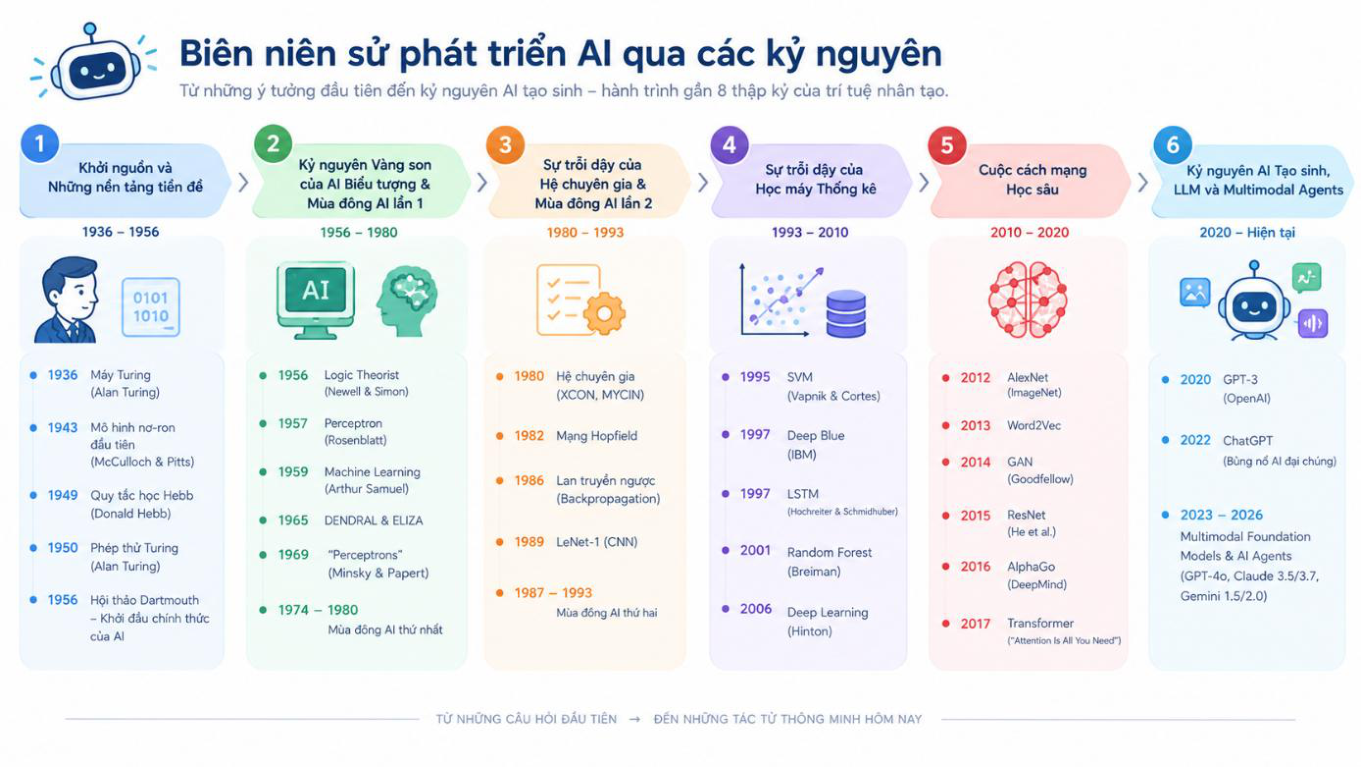
\includegraphics[width=\linewidth,height=.56\textheight,keepaspectratio]{media/media/image1.png}
\caption{Các giai đoạn và quan hệ giữa các kỹ thuật AI}\label{fig:legacy-1.1}
\end{figure}



Giai đoạn 1: Khởi nguồn và Những nền tảng tiền đề (1936 -- 1956)

\begin{quote}
• 1936 --- Máy Turing (Alan Turing): Alan Turing công bố công trình lịch
sử "On Computable Numbers", hình thức hóa khái niệm "thuật toán" và
"tính toán" thông qua cỗ máy trừu tượng Turing Machine. Đây là nền móng
toán học khẳng định khái niệm tính được bằng thuật toán có thể được mô
hình hóa chặt chẽ; điều này không chứng minh mọi hoạt động tư duy đều
tính được.

• 1943 --- Mô hình nơ-ron nhân tạo đầu tiên (Warren McCulloch \& Walter
Pitts): Đề xuất mô hình toán học nhị phân mô phỏng tế bào thần kinh sinh
học, chứng minh rằng một mạng lưới các nơ-ron logic có thể tính toán bất
kỳ hàm logic nào.

• 1949 --- Quy tắc học Hebb (Donald Hebb): Cuốn sách "The Organization
of Behavior" chỉ ra rằng khi hai tế bào thần kinh được kích hoạt đồng
thời, liên kết giữa chúng sẽ mạnh lên ("Cells that fire together, wire
together"). Đây là nguồn gốc của việc điều chỉnh trọng số liên kết trong
mạng nơ-ron.

• 1950 --- Phép thử Turing \& Câu hỏi lịch sử: Alan Turing công bố bài
báo "Computing Machinery and Intelligence", đặt ra câu hỏi bất hủ: "Máy
móc có thể suy nghĩ được không?" và giới thiệu phép thử Turing
(Imitation Game).

• 1956 --- Hội thảo Dartmouth --- Điểm khởi đầu chính thức: John
McCarthy, Marvin Minsky, Nathaniel Rochester và Claude Shannon đồng tổ
chức hội thảo 2 tháng tại Đại học Dartmouth. Thuật ngữ "Artificial
Intelligence" chính thức ra đời, đánh dấu sự hình thành của một ngành
khoa học độc lập.
\end{quote}

Giai đoạn 2: Kỷ nguyên Vàng son của AI Biểu tượng \& Mùa đông AI lần 1
(1956 -- 1980)

\begin{quote}
• 1956 --- Logic Theorist (Newell \& Simon): Chương trình AI đầu tiên có
khả năng chứng minh 38 trong 52 định lý của chương 2 cuốn sách Principia
Mathematica, thậm chí tìm ra cách chứng minh ngắn gọn hơn cả các tác giả
gốc.

• 1957 --- Perceptron (Frank Rosenblatt): Phát minh ra thuật toán
Perceptron -- mô hình học máy đầu tiên có thể học trọng số từ dữ liệu để
phân loại nhị phân trên phần cứng Mark I Perceptron. Rosenblatt tuyên bố
máy sẽ sớm có thể nhìn, nói và tự sinh sản.

• 1959 --- Khái niệm "Machine Learning" (Arthur Samuel): Viết chương
trình chơi cờ đam (checkers) tự cải thiện năng lực qua từng ván đấu và
định nghĩa Machine Learning: "Khoa học giúp máy tính có khả năng tự học
mà không cần được lập trình chi tiết từng bước".

• 1965 --- DENDRAL \& ELIZA (1966): Hệ thống DENDRAL phân tích cấu trúc
phân tử hóa học (tiền thân của hệ chuyên gia); Joseph Weizenbaum phát
triển chatbot ELIZA mô phỏng nhà tâm lý học giao tiếp qua khớp mẫu từ
khóa.

• 1969 --- Cuốn sách "Perceptrons" (Minsky \& Papert): Cuốn sách toán
học chỉ ra giới hạn chết người của Perceptron đơn lớp: hoàn toàn không
thể giải quyết bài toán XOR (bài toán phân tách phi tuyến). Kết luận bi
quan này khiến làn sóng nghiên cứu mạng nơ-ron bị đình trệ nghiêm trọng
suốt hơn một thập kỷ.

• 1974--1980 --- Mùa đông AI thứ nhất (The First AI Winter): Báo cáo
Lighthill (1973) tại Anh và các đánh giá của DARPA tại Mỹ kết luận AI đã
hứa hẹn quá mức so với thực tế ("Bùng nổ tổ hợp", máy tính không đủ bộ
nhớ để giải bài toán ngoài "thế giới đồ chơi"). Tài trợ bị cắt giảm ồ
ạt, các dự án AI bước vào giai đoạn thoái trào sâu rộng.
\end{quote}

Giai đoạn 3: Sự trỗi dậy của Hệ chuyên gia \& Mùa đông AI lần 2 (1980 --
1993)

\begin{quote}
• 1980 --- Sự bùng nổ của Hệ chuyên gia (Expert Systems): AI chuyển
hướng sang AI tri thức biểu tượng. Hệ thống mã hóa tri thức chuyên gia
dưới dạng hàng nghìn luật "NẾU... THÌ...". Hệ thống XCON của Digital
Equipment Corporation (DEC) giúp tiết kiệm 40 triệu USD/năm; MYCIN chẩn
đoán nhiễm trùng máu chính xác ngang chuyên gia hàng đầu.

• 1982 --- Mạng Hopfield (John Hopfield): Giới thiệu mạng nơ-ron hồi quy
có khả năng lưu trữ thông tin như bộ nhớ liên kết (Associative Memory),
làm bừng tỉnh lại cộng đồng nghiên cứu mạng nơ-ron.

• 1986 --- Thuật toán Lan truyền ngược (Backpropagation): David
Rumelhart, Geoffrey Hinton và Ronald Williams xuất bản bài báo kinh điển
trên tạp chí Nature, tái khám phá và phổ biến giải thuật Lan truyền
ngược lỗi cho mạng nơ- ron nhiều lớp. Giới hạn hàm XOR của Minsky chính
thức bị đập tan.

• 1989 --- LeNet-1 (Yann LeCun): Yann LeCun sáng tạo ra mạng nơ-ron tích
chập (CNN) kết hợp lan truyền ngược, ứng dụng thành công trong việc nhận
dạng chữ số viết tay trên séc ngân hàng bưu điện Mỹ.

• 1987--1993 --- Mùa đông AI thứ hai (The Second AI Winter): Các hệ
chuyên gia bộc lộ điểm nghẽn nghiêm trọng: chi phí bảo trì khổng lồ,
"nút thắt thu thập tri thức" (Knowledge Acquisition Bottleneck), hệ
thống giòn giã (brittle) -- thất bại hoàn toàn khi gặp tình huống ngoại
lệ. Thị trường phần cứng chuyên biệt LISP sụp đổ trước sự vươn lên của
PC thương mại. AI một lần nữa rơi vào khủng hoảng lòng tin.
\end{quote}

Giai đoạn 4: Sự trỗi dậy của Học máy Thống kê (1993 -- 2010)

Từ bỏ tham vọng giải quyết trí tuệ tổng quát bằng các luật cứng nhắc, AI
chuyển dịch trọng tâm sang phương pháp thống kê, xác suất và tối ưu hóa
lồi:

\begin{quote}
• 1995 --- Máy vector hỗ trợ (Support Vector Machine -- SVM): Vladimir
Vapnik và Corinna Cortes công bố thuật toán SVM với nguyên lý tối đa hóa
biên phân cách (Margin Maximization) và kỹ thuật Kernel Trick. SVM nhanh
chóng trở thành công cụ phân loại thống trị nhờ cơ sở lý thuyết toán học
vững chắc và tránh được cực tiểu địa phương.

• 1997 --- Deep Blue đánh bại Garry Kasparov: Siêu máy tính Deep Blue
của IBM đánh bại nhà vô địch cờ vua thế giới Garry Kasparov, thu hút sự
chú ý về năng lực tính toán của máy tính.

• 1997 --- Mạng LSTM ra đời (Hochreiter \& Schmidhuber): Sepp Hochreiter
và Jürgen Schmidhuber phát minh kiến trúc Long Short-Term Memory (LSTM),
giảm khó khăn học phụ thuộc dài hạn do biến mất gradient trong mạng RNN,
đặt nền móng cho xử lý chuỗi thời gian và NLP hiện đại.

• 2001 --- Random Forest (Leo Breiman): Đề xuất thuật toán Rừng ngẫu
nhiên kết hợp Bagging và lựa chọn ngẫu nhiên tập đặc trưng, trở thành
một phương pháp thường dùng cho dữ liệu dạng bảng.

• 2006 --- Geoffrey Hinton và "Deep Learning": Hinton cùng các cộng sự
công bố kỹ thuật tiền huấn luyện từng lớp (Layer-wise Pre-training) cho
mạng Deep Belief Networks, góp phần khôi phục quan tâm đến huấn luyện
mạng sâu.
\end{quote}

Giai đoạn 5: Cuộc cách mạng Học sâu (Deep Learning Revolution) (2010 --
2020)

\begin{quote}
• 2012 --- AlexNet và bước ngoặt ImageNet: Alex Krizhevsky, Ilya
Sutskever và Geoffrey Hinton giành chiến thắng áp đảo tại cuộc thi
ILSVRC với mạng CNN 8 lớp mang tên AlexNet, huấn luyện song song trên 2
GPU NVIDIA GTX 580. Tỉ lệ lỗi Top-5 giảm từ 26\% xuống 15.3\%. Khoảnh
khắc này đánh dấu sự ưu thế của mạng sâu trên benchmark này so với các
phương pháp thiết kế đặc trưng thủ công.

• 2013 --- Word2Vec (Tomas Mikolov / Google): Ánh xạ từ ngữ thành vector
ngữ nghĩa trong không gian liên tục (Vector Embedding), nắm bắt quan hệ
ngữ nghĩa tinh tế.

• 2014 --- Mạng sinh đối kháng GAN (Ian Goodfellow): Đề xuất kiến trúc
hai mạng Generator và Discriminator được huấn luyện đối kháng để học
phân phối dữ liệu và tạo mẫu mới.

• 2015 --- Mạng ResNet (Kaiming He et al.): Sáng tạo cơ chế kết nối tắt
(Residual Skip Connections), cho phép huấn luyện thành công các mạng
nơ-ron sâu tới 152 lớp, giảm khó khăn khi tối ưu mạng nhiều tầng.

• 2016 --- AlphaGo đánh bại Lee Sedol: Mô hình AlphaGo (DeepMind) kết
hợp Deep RL và tìm kiếm cây Monte Carlo thắng kỳ thủ cờ vây hàng đầu thế
giới 4- 1, cho thấy khả năng áp dụng học sâu kết hợp tìm kiếm vào cờ vây.

• 2017 --- Kiến trúc Transformer ("Attention Is All You Need"): Đội ngũ
nghiên cứu Google đề xuất kiến trúc Transformer dựa thuần túy trên cơ
chế tự chú ý (Self-Attention), loại bỏ hoàn toàn cấu trúc tuần tự của
RNN trong kiến trúc gốc và là cơ sở cho các mô hình như BERT, GPT.
\end{quote}

Giai đoạn 6: Kỷ nguyên AI Tạo sinh, LLM và Multimodal Agents (2020 --
Hiện tại)

\begin{quote}
• 2020 --- GPT-3 (OpenAI): Mô hình ngôn ngữ với 175 tỉ tham số thể hiện
khả năng học từ một số ví dụ trong ngữ cảnh (Few-shot In-context Learning) mà
không cần tái huấn luyện trọng số.

• 2022 --- ChatGPT và ứng dụng hội thoại: Kết hợp tinh chỉnh chỉ dẫn
(Instruction Tuning) và Học tăng cường từ phản hồi của con người (RLHF),
các hệ hội thoại trở thành một hướng ứng dụng phổ biến, đồng thời đặt ra
những yêu cầu về kiểm chứng thông tin, quyền riêng tư và đánh giá đầu ra.

• Từ 2023: Mô hình nền tảng đa phương thức kết hợp văn bản, hình ảnh và
âm thanh. Các tác tử dùng mô hình ngôn ngữ để lựa chọn công cụ và thực
hiện chuỗi thao tác, đồng thời cần kiểm soát quyền, đánh giá lỗi và giám
sát con người.
\end{quote}

\section{Bản đồ phân loại toàn cảnh các kỹ thuật AI}\label{bux1ea3n-ux111ux1ed3-phuxe2n-loux1ea1i-touxe0n-cux1ea3nh-cuxe1c-kux1ef9-thuux1eadt-ai}

Sơ đồ phân cấp trình bày quan hệ giữa các nhóm phương pháp và phạm vi
ứng dụng của chúng:

\begin{figure}[H]
\centering
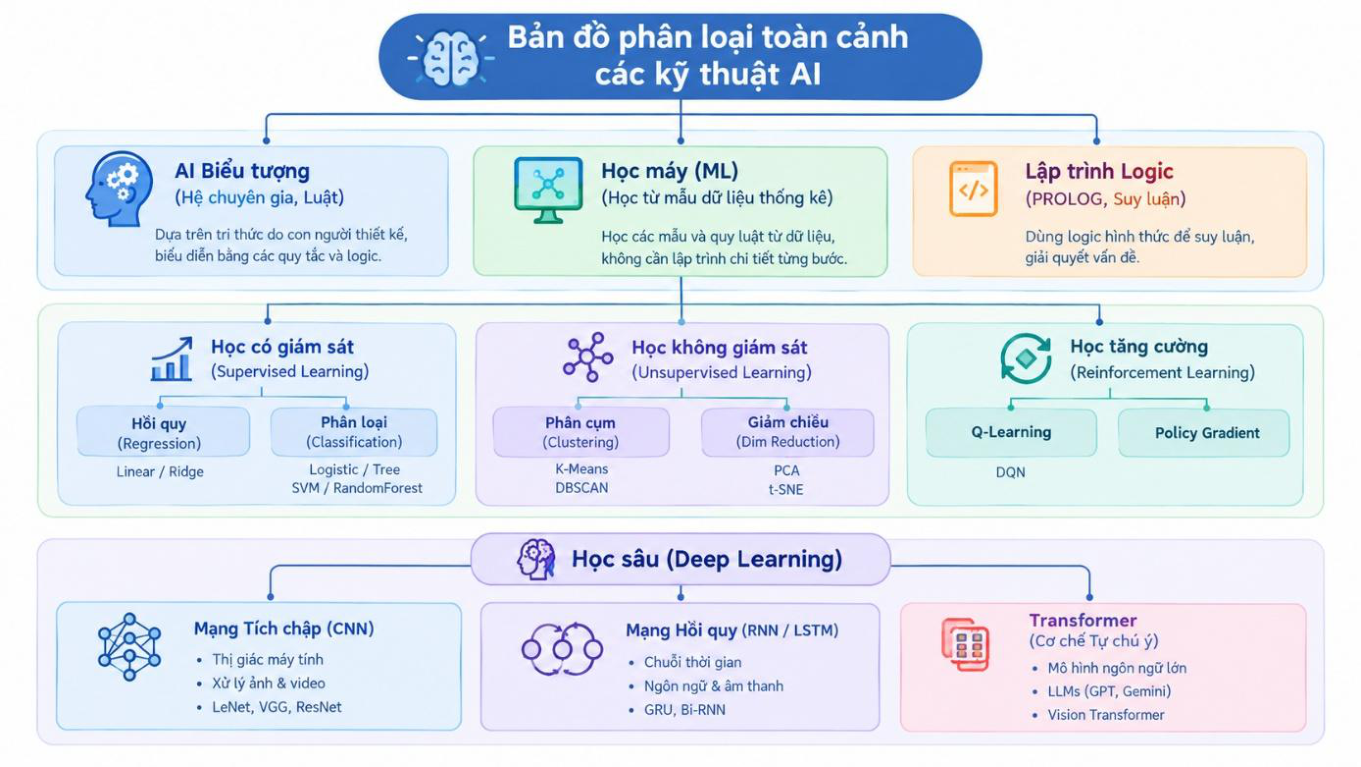
\includegraphics[width=\linewidth,height=.56\textheight,keepaspectratio]{media/media/image2.png}
\caption{Các giai đoạn và quan hệ giữa các kỹ thuật AI}\label{fig:legacy-1.2}
\end{figure}



\section{Ba trụ cột tạo nên sự bùng nổ của Deep Learning sau 2012}\label{ba-trux1ee5-cux1ed9t-tux1ea1o-nuxean-sux1ef1-buxf9ng-nux1ed5-cux1ee7a-deep-learning-sau-2012}

Sự phát triển của học sâu sau năm 2012 gắn với khả năng khai thác dữ liệu
lớn, năng lực tính toán và những tiến bộ về thuật toán. Ba yếu tố này
bổ sung cho nhau trong quá trình huấn luyện mạng:

\Needspace{7\baselineskip}
\captionof{table}{Ba trụ cột phát triển của học sâu}\label{tab:legacy-1.2}

{\def\LTcaptype{none} % do not increment counter
\begin{longtable}[]{@{}
  >{\raggedright\arraybackslash}p{(\linewidth - 4\tabcolsep) * \real{0.1875}}
  >{\raggedright\arraybackslash}p{(\linewidth - 4\tabcolsep) * \real{0.4062}}
  >{\raggedright\arraybackslash}p{(\linewidth - 4\tabcolsep) * \real{0.4062}}@{}}
\toprule\noalign{}
\begin{minipage}[b]{\linewidth}\raggedright
\textbf{Trụ cột}
\end{minipage} & \begin{minipage}[b]{\linewidth}\centering
\textbf{Bản chất kỹ thuật}
\end{minipage} & \begin{minipage}[b]{\linewidth}\centering
\textbf{Cột mốc minh họa}
\end{minipage} \\
\midrule\noalign{}
\endhead
\bottomrule\noalign{}
\endlastfoot
Dữ liệu số khổng lồ & Mạng nơ-ron sâu chứa hàng triệu đến hàng tỷ tham
số, do đó đòi hỏi tập dữ liệu khổng lồ để tránh overfitting và đạt khả
năng tổng quát hóa cao. & Dự án ImageNet gán nhãn hơn 14 triệu hình ảnh,
cung cấp dữ liệu tiêu chuẩn cho mô hình học sâu. \\
Tính toán GPU & Mạng nơ-ron là chuỗi phép nhân ma trận song song; kiến
trúc nhiều nhân của GPU phù hợp hơn CPU truyền thống. & CUDA xuất hiện
năm 2007; AlexNet năm 2012 huấn luyện trên hai GPU GTX 580. \\
Thuật toán và kiến trúc & ReLU, Dropout, BatchNorm, Adam và kết nối tắt
hỗ trợ tối ưu mạng sâu và hạn chế quá khớp. & Dropout (2012), BatchNorm
(2015), Adam (2014), ResNet (2015). \\
\end{longtable}
}

\section{Phân loại AI theo mức độ năng lực và Trường phái tiếp cận}\label{phuxe2n-loux1ea1i-ai-theo-mux1ee9c-ux111ux1ed9-nux103ng-lux1ef1c-vuxe0-trux1b0ux1eddng-phuxe1i-tiux1ebfp-cux1eadn}

\subsection{Phân loại theo cấp độ năng lực}\label{phuxe2n-loux1ea1i-theo-cux1ea5p-ux111ux1ed9-nux103ng-lux1ef1c}

\begin{quote}
• AI Hẹp (Artificial Narrow AI -- ANI): Hệ thống AI được tối ưu hóa xuất
sắc cho một nhiệm vụ duy nhất cụ thể (chơi cờ vây, nhận dạng khuôn mặt,
dịch máy, phân loại ảnh). Mặc dù thể hiện sự vượt trội so với con người
trong miền hẹp, ANI hoàn toàn không có nhận thức hay khả năng tự thích
ứng ngoài phạm vi được huấn luyện. Toàn bộ các hệ thống AI ứng dụng hiện
nay đều thuộc cấp độ này.

• AI Tổng quát (Artificial General Intelligence -- AGI): Hệ thống trí
tuệ nhân tạo giả định có năng lực tư duy, suy luận, tự học và giải quyết
vấn đề linh hoạt tương đương trí tuệ con người trên mọi lĩnh vực tri
thức. Hiện nay, các mô hình nền tảng đa phương thức (Foundation Models)
đang từng bước tiệm cận các khía cạnh nhận thức của AGI nhưng vẫn chưa
đạt tới mục tiêu này.

• Siêu trí tuệ nhân tạo (Artificial Superintelligence -- ASI): Khái niệm
giả thuyết về một hệ thống AI sở hữu năng lực trí tuệ vượt xa những bộ
não xuất sắc nhất của nhân loại ở mọi lĩnh vực khoa học, sáng tạo nghệ
thuật và kỹ năng xã hội.
\end{quote}

\subsection{Hai trường phái tư tưởng lớn trong AI}\label{hai-trux1b0ux1eddng-phuxe1i-tux1b0-tux1b0ux1edfng-lux1edbn-trong-ai}

\begin{quote}
• Trường phái Biểu tượng (Symbolic AI / Good Old-Fashioned AI -- GOFAI):
Tiếp cận theo hướng "từ trên xuống" (Top-down). Trí tuệ được mô hình hóa
bằng các biểu tượng rõ ràng và các phép toán logic hình thức. Ưu điểm là
tính minh
\end{quote}

bạch và suy luận chặt chẽ; nhược điểm là không thể xử lý tốt sự nhiễu
loạn và tính liên tục của thế giới thực.

\begin{quote}
• Trường phái Kết nối (Connectionist AI / Neural Networks): Tiếp cận
theo hướng "từ dưới lên" (Bottom-up). Trí tuệ nảy sinh từ sự tương tác
phức tạp của hàng triệu nơ-ron đơn giản kết nối với nhau, học hỏi trực
tiếp từ mẫu dữ liệu số. Ưu điểm là khả năng thích ứng với dữ liệu phi
cấu trúc; nhược điểm là tính chất "hộp đen" khó diễn giải tường minh.
\end{quote}

\section{Xu hướng AI tại Việt Nam và Những thách thức đương đại}\label{xu-hux1b0ux1edbng-ai-tux1ea1i-viux1ec7t-nam-vuxe0-nhux1eefng-thuxe1ch-thux1ee9c-ux111ux1b0ux1a1ng-ux111ux1ea1i}

\subsection{Bức tranh phát triển AI tại Việt Nam}\label{bux1ee9c-tranh-phuxe1t-triux1ec3n-ai-tux1ea1i-viux1ec7t-nam}

Việt Nam đang có những bước phát triển trong nghiên cứu và ứng dụng trí
tuệ nhân tạo:

\begin{quote}
• Khung chính sách chiến lược: Ban hành Quyết định 127/QĐ-TTg ngày
26/01/2021 về Chiến lược quốc gia về nghiên cứu, phát triển và ứng dụng
AI đến năm 2030, định vị AI là công nghệ nền tảng thúc đẩy chuyển đổi số
quốc gia.

• Trung tâm nghiên cứu \& Doanh nghiệp tiên phong: Sự ra đời của các
viện nghiên cứu trong nước như VinAI Research, Viettel AI, FPT AI
Center, Zalo AI Lab... đã đóng góp nhiều công trình công bố tại các hội
nghị đỉnh cao (NeurIPS, CVPR, ICML) và thương mại hóa các giải pháp trợ
lý ảo tiếng Việt, xe tự hành, camera thông minh.

• Ứng dụng thực tiễn: Tích hợp AI vào hành chính công, chẩn đoán y tế từ
xa, nông nghiệp công nghệ cao và phòng chống thiên tai.
\end{quote}

\subsection{Những thách thức cốt lõi đặt ra}\label{nhux1eefng-thuxe1ch-thux1ee9c-cux1ed1t-luxf5i-ux111ux1eb7t-ra}

1. Tính chất "Hộp đen" \& Khả năng giải thích (Explainable AI -- XAI):
Các mạng nơ-ron sâu đưa ra dự báo chính xác nhưng con người khó truy
xuất lý do tại sao, gây rủi ro lớn trong các lĩnh vực nhạy cảm như chẩn
đoán ung thư, phê duyệt tín dụng hay tư pháp.

2. Thiên lệch dữ liệu \& Tính công bằng (Data Bias \& Fairness): Mô hình
học từ dữ liệu lịch sử của con người nên có nguy cơ phản ánh và khuếch
đại các định kiến xã hội về giới tính, chủng tộc hoặc địa lý.

3. Độ tin cậy \& Hiện tượng "Ảo giác" (Hallucination): Các mô hình ngôn
ngữ lớn có xu hướng sinh ra thông tin sai lệch nhưng với giọng điệu vô
cùng tự tin, gây nguy hại cho việc tiếp nhận tri thức chính xác.

4. Chi phí tính toán \& Tác động môi trường (Compute Cost \& Green AI):
Huấn luyện một mô hình nền tảng hiện đại tiêu tốn hàng chục triệu USD và
năng lượng đáng kể, phụ thuộc quy mô và phần cứng, đặt ra bài toán về
tính bền vững và sự bất bình đẳng công nghệ giữa các quốc gia.

5. Quyền riêng tư dữ liệu \& An toàn bảo mật (Privacy \& Adversarial
Robustness): Nguy cơ rò rỉ dữ liệu cá nhân khi huấn luyện mô hình và khả
năng mô hình bị đánh lừa bởi các cuộc tấn công đối nghịch (Adversarial
Attacks).

\section{Mối liên hệ giữa các giai đoạn phát triển}\label{mux1ed1i-liuxean-hux1ec7-giux1eefa-cuxe1c-giai-ux111oux1ea1n-phuxe1t-triux1ec3n}

AI biểu tượng cung cấp cách biểu diễn tri thức và suy luận có thể kiểm
tra. Học máy thống kê chuyển trọng tâm sang việc học quy luật từ dữ
liệu; học sâu tiếp tục học biểu diễn thay cho nhiều bước thiết kế đặc
trưng thủ công. Transformer cho phép mô hình hóa quan hệ giữa các vị trí
qua attention và huấn luyện song song hơn RNN. KG và RAG kết nối mô hình
dữ liệu với tri thức tường minh; chúng kế thừa các ý tưởng cũ thay vì
thay thế toàn bộ AI biểu tượng.

Trong báo cáo này, mối liên hệ đó được thể hiện bằng ba loại đầu vào:
bảng thuộc tính, ảnh và chuỗi thời gian. Các mô hình tạo ra dự đoán định
lượng; Chương 5 bổ sung bằng chứng và ngữ cảnh để người dùng hiểu phạm
vi của các kết quả.

\subsection{Từ biểu diễn tri thức đến biểu diễn học được}\label{tux1eeb-biux1ec3u-diux1ec5n-tri-thux1ee9c-ux111ux1ebfn-biux1ec3u-diux1ec5n-hux1ecdc-ux111ux1b0ux1ee3c}

Với một bộ luật, người thiết kế xác định trước thuộc tính và điều kiện
suy luận. Cách làm này thuận lợi khi quy tắc rõ và miền tri thức ổn
định, nhưng số trường hợp cần mô tả tăng nhanh khi đầu vào đa dạng. Học
máy chuyển một phần công việc sang dữ liệu: mô hình ước lượng quan hệ
giữa các đặc trưng và nhãn. Học sâu tiếp tục thay đổi ở cấp biểu diễn,
chẳng hạn tự học kernel từ pixel thay vì yêu cầu liệt kê thủ công mọi
nét đặc trưng của chữ số.

Sự chuyển dịch không có nghĩa tri thức tường minh mất vai trò. Trong bài
toán sức khỏe, quy định về đơn vị, phạm vi sử dụng và cảnh báo không
được suy ra chỉ từ nhãn của một tập dữ liệu tổng hợp. Trong bài toán thị
trường, quan hệ giữa mã tài sản, loại dữ liệu và chỉ báo cần được ghi rõ
để tránh gọi vàng futures thành vàng giao ngay. Những ràng buộc này nằm
ngoài một giá trị dự đoán đơn lẻ và phù hợp với biểu diễn có cấu trúc.

\subsection{Tiêu chí lựa chọn công nghệ trong hệ thống}\label{tiuxeau-chuxed-lux1ef1a-chux1ecdn-cuxf4ng-nghux1ec7-trong-hux1ec7-thux1ed1ng}

\Needspace{7\baselineskip}
\captionof{table}{Liên hệ giữa đặc điểm đầu vào và lựa chọn kỹ thuật}\label{tab:legacy-1.3}

{\def\LTcaptype{none} % do not increment counter
\begin{longtable}[]{@{}
  >{\raggedright\arraybackslash}p{(\linewidth - 4\tabcolsep) * \real{0.2000}}
  >{\raggedright\arraybackslash}p{(\linewidth - 4\tabcolsep) * \real{0.3750}}
  >{\raggedright\arraybackslash}p{(\linewidth - 4\tabcolsep) * \real{0.4250}}@{}}
\toprule\noalign{}
\begin{minipage}[b]{\linewidth}\raggedright
\textbf{Dạng đầu vào}
\end{minipage} & \begin{minipage}[b]{\linewidth}\centering
\textbf{Vấn đề cần giải quyết}
\end{minipage} & \begin{minipage}[b]{\linewidth}\centering
\textbf{Lựa chọn trong project}
\end{minipage} \\
\midrule\noalign{}
\endhead
\bottomrule\noalign{}
\endlastfoot
Bảng thuộc tính & Giá trị thiếu, quan hệ phi tuyến, lớp hiếm & Pipeline
tiền xử lý và Random Forest \\
Ảnh xám & Tương quan cục bộ, nét xuất hiện ở nhiều vị trí & CNN có
kernel dùng chung \\
Chuỗi theo phiên & Thông tin quá khứ và phụ thuộc thứ tự & RNN/LSTM/GRU;
đối chiếu Persistence \\
Câu hỏi và tri thức & Tìm bằng chứng phù hợp, giữ quan hệ thực thể &
TF-IDF/BM25 và Knowledge Graph \\
\end{longtable}
}

Các chương sau dùng cùng nguyên tắc kiểm tra: xác định đúng bài toán
trước, xây mốc so sánh đơn giản, khóa phần dữ liệu dùng đánh giá và chỉ
sau đó mới tăng độ phức tạp. Một mạng sâu không được ưu tiên chỉ vì có
nhiều tham số; một câu trả lời không được coi là đúng chỉ vì có điểm
truy xuất cao. Giá trị của hệ thống được xem xét đồng thời ở sai số, khả
năng kiểm tra và sự phù hợp với nhu cầu sử dụng.

\section{Tiểu kết chương 1}\label{tiux1ec3u-kux1ebft-chux1b0ux1a1ng-1}

Lịch sử AI thể hiện sự chuyển đổi giữa nhiều hướng tiếp cận: từ các nền
tảng lý thuyết của Alan Turing và Perceptron, qua những giai đoạn suy
giảm đầu tư, đến học máy thống kê và học sâu. Các bước tiến gắn với thay
đổi về dữ liệu, năng lực tính toán và phương pháp học.

Không có một mô hình đơn lẻ phù hợp với mọi bài toán. Việc lựa chọn cần
dựa trên cấu trúc dữ liệu, mục tiêu đánh giá và khả năng kiểm tra kết
quả, từ các kỹ thuật học máy cho bảng thuộc tính đến kiến trúc chuyên
biệt cho ảnh và chuỗi.

Chương tiếp theo cụ thể hóa các nguyên tắc trên bằng hai bài toán dữ
liệu bảng, trong đó phép chia dữ liệu và lựa chọn thước đo được xác định
trước khi so sánh mô hình.

\chapter{Các kỹ thuật machine learning cơ bản}\label{chux1b0ux1a1ng-2.-cuxe1c-kux1ef9-thuux1eadt-machine-learning-cux1a1-bux1ea3n}

Trong nhiều ứng dụng, thông tin đầu vào không phải ảnh hay văn bản dài
mà là một bảng thuộc tính. Vấn đề đặt ra là chọn những biến nào, xử lý
giá trị thiếu ra sao và đánh giá thế nào để kết quả không chỉ đúng trên
các bản ghi đã thấy. Một quy trình học máy thiếu kiểm soát phép chia dữ
liệu có thể tạo điểm số cao nhưng không sử dụng được cho mẫu mới.

Hai bài toán được triển khai trong chương là phân loại nhãn nguy cơ tổng
hợp và ước lượng giá nhà từ thông tin tin đăng. Bài toán thứ nhất có lớp
hiếm nên cần xem đồng thời precision, recall và macro-F1; bài toán thứ
hai có nhiều bản ghi cùng địa chỉ nên cần chia theo nhóm. Đây là hai
tình huống giúp làm rõ quan hệ giữa đặc điểm dữ liệu và thiết kế thực
nghiệm.

Sau phần nền tảng, chương lần lượt xác định đầu vào và đầu ra, kiểm tra
dữ liệu, xây pipeline tiền xử lý, so sánh mô hình bằng kiểm định chéo và
phân tích lỗi trên tập test giữ riêng. Cuối chương trình bày cách sử
dụng từng mô hình trên web và giới hạn của kết quả, thay vì coi giao
diện dự đoán là bằng chứng cho độ chính xác.

\section{Cơ sở lý thuyết Học máy (Machine Learning Foundations)}\label{cux1a1-sux1edf-luxfd-thuyux1ebft-hux1ecdc-muxe1y-machine-learning-foundations}

\subsection{Khái niệm và Các dạng học máy}\label{khuxe1i-niux1ec7m-vuxe0-cuxe1c-dux1ea1ng-hux1ecdc-muxe1y}

Năm 1997, Tom Mitchell đã đưa ra định nghĩa toán học chuẩn tắc về học
máy:

"Một chương trình máy tính được coi là học từ kinh nghiệm E đối với một
lớp tác vụ T và thước đo hiệu năng P, nếu hiệu năng của nó đối với các
tác vụ trong T, được đo bằng P, cải thiện theo kinh nghiệm E."

Dựa vào bản chất của kinh nghiệm E (dữ liệu đầu vào), học máy được chia
thành 4 dạng thức chính:

1. Học có giám sát (Supervised Learning):

\begin{quote}
• Dữ liệu huấn luyện bao gồm cặp mẫu đầu vào và nhãn mục tiêu tương ứng:
\end{quote}

\(D = \{(x_{i},y_{i})\}_{i = 1}^{N}\) (2.1)

\begin{quote}
• Mục tiêu: Tìm hàm ánh xạ từ không gian đầu vào sang không gian đầu ra
sao cho dự báo xấp xỉ nhãn thực tế.
\end{quote}

\(f:\mathcal{X} \rightarrow \mathcal{Y},\quad\quad\hat{y} = f(x)\) (2.2)

\begin{quote}
• Hồi quy (Regression): Khi nhãn y thuộc tập số thực, đầu ra là giá trị
liên tục (ví dụ: dự báo giá nhà, nhiệt độ, doanh thu).

• Phân loại (Classification): Khi nhãn là các nhãn lớp rời rạc (ví dụ:
chẩn đoán bệnh tật, phân loại email rác).
\end{quote}

2. Học không giám sát (Unsupervised Learning):

\begin{quote}
• Dữ liệu huấn luyện chỉ bao gồm các mẫu đầu vào mà không có nhãn đích:
\end{quote}

\(D = \{ x_{i}\}_{i = 1}^{N}\) (2.3)

\begin{quote}
• Mục tiêu: Tự động khám phá cấu trúc ẩn sâu bên trong dữ liệu.

• Phân cụm (Clustering): Gom các điểm dữ liệu có đặc trưng tương đồng
vào cùng nhóm (K-Means, DBSCAN).

• Giảm chiều dữ liệu (Dimensionality Reduction): Nén không gian dữ liệu
nhiều chiều xuống không gian ít chiều hơn mà vẫn bảo toàn tối đa thông
tin quan trọng (PCA, t-SNE).
\end{quote}

3. Học bán giám sát \& Tự giám sát (Semi-supervised \& Self-supervised
Learning):

\begin{quote}
• Học bán giám sát: Kết hợp một lượng nhỏ dữ liệu có gán nhãn với một
khối lượng khổng lồ dữ liệu không gán nhãn để tiết kiệm chi phí dán nhãn
thủ công.

• Học tự giám sát: Mô hình tự động tạo ra nhãn từ chính cấu trúc nội tại
của dữ liệu (ví dụ: che giấu một từ trong câu và bắt mô hình dự đoán từ
bị che, tạo tiền đề cho các mô hình ngôn ngữ lớn LLM).
\end{quote}

4. Học tăng cường (Reinforcement Learning -- RL):

\begin{quote}
• Tác tử (Agent) tương tác liên tục với môi trường (Environment) qua các
trạng thái st, thực hiện hành động at và nhận lại tín hiệu phần thưởng
rt
\end{quote}

(Reward). Mục tiêu là tìm chính sách hành động π(a\textbar s) tối đa hóa
tổng phần thưởng tích lũy dài hạn.

\subsection{Quy trình chuẩn xây dựng một mô hình Học máy}\label{quy-truxecnh-chuux1ea9n-xuxe2y-dux1ef1ng-mux1ed9t-muxf4-huxecnh-hux1ecdc-muxe1y}

Một quy trình khoa học dữ liệu hoàn chỉnh bao gồm 5 giai đoạn liên hoàn
khép kín:

{[}1. Thu thập dữ liệu{]} → {[}2. Tiền xử lý (EDA, Clean, Scale){]} →
{[}3. Phân chia Train/Val/Test{]} → {[}4. Huấn luyện \& Tối ưu Siêu tham
số{]} → {[}5. Đánh giá \& Giám sát{]}

1. Thu thập và Khám phá Dữ liệu (EDA): Phân tích phân phối thống kê,
phát hiện ngoại lai (Outliers), kiểm tra độ tương quan giữa các biến và
nhận diện hiện tượng rò rỉ dữ liệu (Data Leakage).

2. Tiền xử lý Dữ liệu:

\begin{quote}
• Xử lý dữ liệu khuyết: Điền khuyết (Imputation) bằng giá trị trung bình
(mean), trung vị (median) hoặc mô hình học máy.

• Mã hóa biến phân loại: One-Hot Encoding cho biến định danh không thứ
bậc, Label Encoding cho biến có thứ bậc.

• Chuẩn hóa thang đo: Đưa các thuộc tính về cùng một miền giá trị bằng
Standard Scaling hoặc Min-Max Scaling nhằm giúp các thuật toán hạ
gradient hội tụ nhanh và ổn định.
\end{quote}

\(z = \frac{x - \mu}{\sigma},\quad\quad x' = \frac{x - x_{\min}}{x_{\max} - x_{\min}}\)
(2.4)

x là giá trị gốc; μ, σ, x\_min và x\_max lần lượt là trung bình, độ lệch
chuẩn và hai biên của đặc trưng. Các đại lượng này chỉ được ước lượng từ
train, rồi giữ cố định khi biến đổi validation/test.

3. Phân chia tập dữ liệu: Chia tách độc lập thành tập Huấn luyện (Train
set), tập Kiểm định (Validation set) và tập Kiểm thử (Test set). Áp dụng
kỹ thuật Kiểm định chéo K-lần (K-Fold Cross-Validation) để đánh giá độ
ổn định của mô hình.

4. Huấn luyện và Tối ưu hóa: Lựa chọn kiến trúc thuật toán phù hợp, định
nghĩa hàm mục tiêu (Loss function) và tinh chỉnh siêu tham số
(Hyperparameter Tuning).

5. Đánh giá và Kiểm định độc lập: Đo lường hiệu năng trên tập Test chưa
từng nhìn thấy bằng các thước đo chuẩn mực.

\subsection{Phương pháp Tối ưu hóa bằng Hạ Gradient (Gradient Descent)}\label{phux1b0ux1a1ng-phuxe1p-tux1ed1i-ux1b0u-huxf3a-bux1eb1ng-hux1ea1-gradient-gradient-descent}

Hạ gradient là thuật toán tối ưu hóa nền tảng trong toàn bộ học máy và
học sâu, nhằm tìm bộ tham số w làm cực tiểu hóa hàm mất mát L(w).

Nguyên lý toán học: Vector gradient \ensuremath{\nabla}L(w) chỉ hướng tăng nhanh nhất của
hàm số tại điểm khảo sát. Do đó, để làm giảm hàm mất mát nhanh nhất, ta
cập nhật tham số ngược hướng với vector gradient:

\(w_{t + 1} = w_{t} - \eta\nabla\mathcal{L}(w_{t})\) (2.5)

Trong đó η\textgreater{} 0 là tốc độ học (Learning Rate). Nếu quá nhỏ,
mô hình hội tụ rất chậm chạp; nếu η quá lớn, mô hình sẽ dao động phân kỳ
và không thể đạt tới điểm cực tiểu.

Các biến thể của Gradient Descent:

\begin{quote}
• Batch Gradient Descent: Tính toán gradient trên toàn bộ mẫu dữ liệu
của tập huấn luyện. Hướng đi rất ổn định nhưng rất tốn bộ nhớ và chậm
chạp khi dữ liệu lớn.

• Stochastic Gradient Descent (SGD): Tính toán gradient và cập nhật tham
số trên từng mẫu đơn lẻ (N = 1). Rất nhanh và có khả năng thoát khỏi các
điểm cực tiểu địa phương cạn, nhưng dao động gradient rất mạnh (nhiễu).

• Mini-batch Gradient Descent: Cân bằng giữa hai thái cực trên bằng cách
chia dữ liệu thành từng nhóm nhỏ kích thước B (thường là 32, 64, 128
mẫu). Đây là cách làm phổ biến trong huấn luyện mạng nơ-ron hiện đại.
\end{quote}

\subsection{Hồi quy tuyến tính (Linear Regression)}\label{hux1ed3i-quy-tuyux1ebfn-tuxednh-linear-regression}

Mô hình hồi quy tuyến tính giả thiết mối quan hệ giữa biến đầu vào x=
{[}x1, x2,..., xd{]}T và biến mục tiêu liên tục y là tuyến tính:

\(\hat{y} = w^{T}x + b = \sum_{j = 1}^{d}w_{j}x_{j} + b\) (2.6)

Hàm mất mát --- Sai số bình phương trung bình (Mean Squared Error --
MSE):

\(\mathcal{L} = \frac{1}{N}\sum_{i = 1}^{N}({\hat{y}}_{i} - y_{i})^{2}\)
(2.7)

Đạo hàm và Cập nhật trọng số: Đạo hàm riêng theo trọng số w:

\(\frac{\partial\mathcal{L}}{\partial w} = \frac{2}{N}X^{T}(\hat{y} - y)\)
(2.8)

Cập nhật tham số qua gradient descent:

\(w \leftarrow w - \eta\frac{\partial\mathcal{L}}{\partial w}\) (2.9)

\subsection{Hồi quy Logistic (Logistic Regression \& Softmax)}\label{hux1ed3i-quy-logistic-logistic-regression-softmax}

Dành cho bài toán phân loại. Dù mang tên "hồi quy", mô hình này thực
chất là một bộ phân loại tuyến tính xác suất.

Phân loại nhị phân (Binary Classification): Để ép giá trị đầu ra tuyến
tính z= wTx+ b về khoảng xác suất, mô hình sử dụng hàm kích hoạt
Sigmoid:

\(\sigma(z) = \frac{1}{1 + e^{- z}}\) (2.10)

Hàm mất mát --- Binary Cross-Entropy (BCE / Log Loss):

\(\mathcal{L}_{BCE} = - \frac{1}{N}\sum_{i = 1}^{N}\lbrack y_{i}\log{\hat{y}}_{i} + (1 - y_{i})\log(1 - {\hat{y}}_{i})\rbrack\)
(2.11)

Phân loại đa lớp (Multiclass Classification --- Softmax Regression): Khi
có K lớp phân loại rời rạc, đầu ra tại lớp thứ k được chuẩn hóa qua hàm
Softmax:

\(p_{k} = \frac{e^{z_{k}}}{\sum_{j = 1}^{K}e^{z_{j}}}\) (2.12)

Hàm mất mát tương ứng là Categorical Cross-Entropy:

\(\mathcal{L}_{CE} = - \frac{1}{N}\sum_{i = 1}^{N}{\sum_{k = 1}^{K}y_{ik}}\log p_{ik}\)
(2.13)

\subsection{Tổng quan các thuật toán Học máy kinh điển tiêu biểu}\label{tux1ed5ng-quan-cuxe1c-thuux1eadt-touxe1n-hux1ecdc-muxe1y-kinh-ux111iux1ec3n-tiuxeau-biux1ec3u}

Bên cạnh các mô hình tuyến tính, học máy cổ điển sở hữu các thuật toán
phi tuyến xuất sắc:

1. Cây quyết định (Decision Tree):

\begin{quote}
• Phân chia không gian dữ liệu bằng các câu hỏi điều kiện phân nhánh nhị
phân trực quan.

• Tiêu chuẩn phân chia tối ưu: sử dụng độ lợi thông tin (Information
Gain) dựa trên Entropy hoặc chỉ số Gini Impurity.
\end{quote}

\(H(S) = - \sum_{k = 1}^{K}p_{k}\log_{2}p_{k},\quad\quad G(S) = 1 - \sum_{k = 1}^{K}p_{k}^{2}\)
(2.14)

pk là tỷ lệ mẫu thuộc lớp k ở nút đang xét. Độ lợi thông tin là độ giảm
entropy có trọng số sau khi chia. Một phép chia có độ lợi cao tạo các
nút con đồng nhất hơn về nhãn.

\begin{quote}
• Ưu điểm: Rất dễ giải thích, không yêu cầu chuẩn hóa thang đo; Nhược
điểm: Dễ bị quá khớp (Overfitting) nếu cây phát triển quá sâu.
\end{quote}

2. Phương pháp Tổ hợp (Ensemble Methods):

\begin{quote}
• Rừng ngẫu nhiên (Random Forest): Kỹ thuật đóng gói (Bagging) kết hợp
dự báo của hàng trăm cây quyết định độc lập được huấn luyện trên các tập
mẫu con lấy mẫu có hoàn lại (Bootstrap) và tập thuộc tính ngẫu nhiên.
Giảm phương sai, rất bền bỉ và chính xác trên dữ liệu dạng bảng.

• Gradient Boosting (GBM / XGBoost / LightGBM): Kỹ thuật tăng cường
(Boosting) xây dựng các cây quyết định tuần tự, trong đó mỗi cây sau tập
trung sửa chữa sai số (Residuals) của các cây trước đó. Thường đạt độ
chính xác cao nhất trong các cuộc thi dữ liệu bảng.
\end{quote}

3. Máy vector hỗ trợ (Support Vector Machine -- SVM):

\begin{quote}
• Tìm kiếm siêu phẳng phân cách tối ưu sao cho khoảng cách (lề - margin)
từ siêu phẳng tới các điểm dữ liệu gần nhất của hai lớp (gọi là các
Support Vectors) là cực đại.

• Kernel Trick: Ánh xạ dữ liệu không phân tách tuyến tính từ không gian
gốc lên không gian nhiều chiều hơn thông qua các hàm nhân (RBF Kernel,
Polynomial Kernel) để phân tách tuyến tính mà không cần tính toán tọa độ
rõ ràng.
\end{quote}

4. K láng giềng gần nhất (K-Nearest Neighbors -- KNN):

\begin{quote}
• Giải thuật học lười biếng (Lazy Learning): Không có pha huấn luyện
tường minh. Khi dự báo mẫu mới, thuật toán tính khoảng cách (Euclidean,
Manhattan) tới toàn bộ các điểm trong tập dữ liệu và lấy biểu quyết đa
số từ K điểm láng giềng gần nhất.
\end{quote}

\Needspace{7\baselineskip}
\captionof{table}{So sánh các thuật toán học máy kinh điển}\label{tab:legacy-2.1}

{\def\LTcaptype{none} % do not increment counter
\begin{longtable}[]{@{}
  >{\raggedright\arraybackslash}p{(\linewidth - 10\tabcolsep) * \real{0.1625}}
  >{\centering\arraybackslash}p{(\linewidth - 10\tabcolsep) * \real{0.1438}}
  >{\centering\arraybackslash}p{(\linewidth - 10\tabcolsep) * \real{0.1501}}
  >{\centering\arraybackslash}p{(\linewidth - 10\tabcolsep) * \real{0.1937}}
  >{\raggedright\arraybackslash}p{(\linewidth - 10\tabcolsep) * \real{0.1750}}
  >{\centering\arraybackslash}p{(\linewidth - 10\tabcolsep) * \real{0.1750}}@{}}
\toprule\noalign{}
\begin{minipage}[b]{\linewidth}\raggedright
\textbf{Thuật toán}
\end{minipage} & \begin{minipage}[b]{\linewidth}\centering
\textbf{Bản chất}
\end{minipage} & \begin{minipage}[b]{\linewidth}\centering
\textbf{Độ phức tạp}
\end{minipage} & \begin{minipage}[b]{\linewidth}\centering
\textbf{Giải thích}
\end{minipage} & \begin{minipage}[b]{\linewidth}\centering
\textbf{Ưu điểm}
\end{minipage} & \begin{minipage}[b]{\linewidth}\centering
\textbf{Hạn chế}
\end{minipage} \\
\midrule\noalign{}
\endhead
\bottomrule\noalign{}
\endlastfoot
Logistic Regression & Tuyến tính + Sigmoid & Dự đoán O(d) & Hệ số trọng
số & Đơn giản, nhanh; xuất xác suất & Biên phân cách tuyến tính \\
Decision Tree & Cắt lát không gian & Phụ thuộc độ sâu & Cây luật
NẾU--THÌ & Trực quan; ít cần scaling & Dễ quá khớp, nhạy nhiễu \\
Random Forest & Bagging nhiều cây & Phụ thuộc số cây, N, d và độ sâu &
Feature importance & Bền bỉ, giảm phương sai & Mô hình lớn hơn, dự báo
chậm hơn \\
Gradient Boosting & Boosting sửa sai số & Phụ thuộc số vòng và độ sâu &
Trung bình & Mạnh với dữ liệu bảng & Nhạy siêu tham số, tốn thời gian \\
SVM & Cực đại hóa margin & Phụ thuộc kernel và số mẫu & Thấp với kernel
& Mạnh với ít mẫu, nhiều chiều & Chậm trên tập lớn \\
KNN & Khoảng cách mẫu & Brute-force O(Nd) mỗi truy vấn & Láng giềng &
Trực quan, không giả định phân phối & Tốn bộ nhớ, dự báo chậm \\
\end{longtable}
}

\subsection{Hiện tượng Overfitting, Underfitting \& Kỹ thuật Điều chuẩn}\label{hiux1ec7n-tux1b0ux1ee3ng-overfitting-underfitting-kux1ef9-thuux1eadt-ux111iux1ec1u-chuux1ea9n}

Sự đánh đổi giữa Độ chệch và Phương sai (Bias-Variance Trade-off): Tổng
sai số kỳ vọng của một mô hình học máy được phân rã thành 3 thành phần:

\(E\lbrack(y - \hat{f}(x))^{2}\rbrack = Bias\lbrack\hat{f}(x)\rbrack^{2} + Var\lbrack\hat{f}(x)\rbrack + \sigma^{2}\)
(2.15)

\begin{quote}
• Thiếu khớp (Underfitting - High Bias): Mô hình quá đơn giản, không học
đủ quy luật từ dữ liệu, sai số trên cả tập Train và Test đều cao.

• Quá khớp (Overfitting - High Variance): Mô hình quá phức tạp, ghi nhớ
cả các nhiễu ngẫu nhiên của tập Train, dẫn tới sai số tập Train cực thấp
nhưng sai số tập Test vọt lên rất cao.
\end{quote}

Các kỹ thuật Điều chuẩn (Regularization): Điều chuẩn là kỹ thuật thêm
một số hạng phạt vào hàm mất mát nhằm hạn chế độ lớn của các trọng số,
ép mô hình đơn giản hơn:

\begin{quote}
• Điều chuẩn L2 (Ridge Regression / Weight Decay): Phạt tổng bình phương
trọng số. Thu nhỏ trọng số về gần 0 nhưng không triệt tiêu hoàn toàn.
\end{quote}

\(\mathcal{L}_{reg} = \mathcal{L} + \lambda\sum_{i}^{}w_{i}^{2}\) (2.16)

\begin{quote}
• Điều chuẩn L1 (Lasso Regression): Phạt tổng giá trị tuyệt đối của
trọng số. Có khả năng triệt tiêu trọng số về chính xác bằng 0, đóng vai
trò chọn lọc đặc trưng tự động.
\end{quote}

\(\mathcal{L}_{reg} = \mathcal{L} + \lambda\sum_{i}^{}|w_{i}|\) (2.17)

\begin{quote}
• Trong Mạng Nơ-ron: Áp dụng kỹ thuật Dropout (ngẫu nhiên ngắt kết nối
một tỉ lệ nơ-ron trong quá trình train để chống đồng thích nghi) và
Early Stopping (dừng huấn luyện khi sai số trên tập Validation bắt đầu
tăng liên tục).
\end{quote}

\subsection{Từ Học máy truyền thống đến Mạng Nơ-ron Sâu (Deep Neural Network -- DNN)}\label{tux1eeb-hux1ecdc-muxe1y-truyux1ec1n-thux1ed1ng-ux111ux1ebfn-mux1ea1ng-nux1a1-ron-suxe2u-deep-neural-network-dnn}

Khi dữ liệu có độ phức tạp cao và phi tuyến mạnh mẽ, việc kết hợp các
tầng biến đổi tuyến tính xen kẽ các hàm kích hoạt phi tuyến dẫn tới kiến
trúc Mạng nơ-ron sâu (DNN).

Có thể minh họa lý thuyết bằng một kiến trúc Mạng nơ-ron sâu 5 lớp (gồm
4 lớp ẩn Dense liên kết đầy đủ + 1 lớp đầu ra):

Input (X) ──► {[}Dense 1 + ReLU{]} ──► {[}Dense 2 + ReLU{]} ──► {[}Dense
3 + ReLU{]} ──► {[}Dense 4 + ReLU{]} ──► Output Layer (ŷ)

1. Lan truyền xuôi (Forward Propagation): Tại mỗi tầng ẩn l\ensuremath{\in}\{1,2,3,4\}:

\(z^{(l)} = W^{(l)}a^{(l - 1)} + b^{(l)},\quad a^{(l)} = ReLU(z^{(l)})\)
(2.18)

Tại tầng đầu ra l = 5:

\begin{quote}
• Với bài toán hồi quy (Housing Price): ŷ = z(5)(kích hoạt tuyến tính).

• Với bài toán phân loại đa lớp: ŷ = Softmax(z(5)).
\end{quote}

2. Lan truyền ngược (Backpropagation theo Chain Rule): Để cập nhật ma
trận trọng số, ta tính toán gradient sai số từ tầng cuối cùng lội ngược
về tầng đầu theo quy tắc chuỗi giải tích:

\(\frac{\partial\mathcal{L}}{\partial W^{(l)}} = \delta^{(l)}(a^{(l - 1)})^{T}\)
(2.19)

\(\delta^{(l)} = ((W^{(l + 1)})^{T}\delta^{(l + 1)}) \odot {ReLU}'(z^{(l)})\)
(2.20)

Trong đó δ là sai số lan truyền ngược. Quy tắc chuỗi cho phép truyền
gradient qua các lớp; phần thực nghiệm mới sử dụng các mô hình được mô
tả riêng bên dưới.

\subsection{Kiểm định chéo và lựa chọn siêu tham số}\label{kiux1ec3m-ux111ux1ecbnh-chuxe9o-vuxe0-lux1ef1a-chux1ecdn-siuxeau-tham-sux1ed1}

Train dùng để ước lượng tham số; validation dùng để kiểm tra các lựa
chọn phát triển và checkpoint; test chỉ dùng cho đánh giá cuối. Trong
phân loại, StratifiedKFold giữ tỷ lệ lớp trong từng fold. Với giá nhà,
GroupKFold giữ các bản ghi cùng địa chỉ trong một fold. Toàn bộ
imputation, scaling và one-hot encoding được fit bên trong từng fold,
không fit trên toàn bộ dữ liệu trước khi chia.

Grid search so sánh tập siêu tham số hữu hạn đã định trước. Dùng
macro-F1 khi các lớp mất cân bằng và MAE theo tỷ VND khi dự báo giá nhà.
Không lựa chọn mô hình bằng chỉ số test. Khoảng cách
train--validation--test giúp phát hiện quá khớp; một lần chia và một
random seed chưa mô tả hết độ bất định.

\subsection{Các thước đo đánh giá}\label{cuxe1c-thux1b0ux1edbc-ux111o-ux111uxe1nh-giuxe1}

\(MAE = \frac{1}{n}\sum_{i = 1}^{n}|y_{i} - {\hat{y}}_{i}|,\quad MSE = \frac{1}{n}\sum_{i = 1}^{n}(y_{i} - {\hat{y}}_{i})^{2}\)
(2.21)

\(RMSE = \sqrt{MSE},\quad R^{2} = 1 - \frac{\sum_{i}^{}(y_{i} - {\hat{y}}_{i})^{2}}{\sum_{i}^{}(y_{i} - \bar{y})^{2}}\)
(2.22)

Trong (2.21)--(2.22), n là số mẫu, yi là giá trị thực, ŷi là dự đoán và
ȳ là trung bình của nhãn trong tập đánh giá. MAE và RMSE có cùng đơn vị
với nhãn, MSE có đơn vị bình phương. R2 so với dự đoán hằng bằng trung
bình, có thể âm và không phải phần trăm chính xác.

\(Accuracy = \frac{TP + TN}{TP + TN + FP + FN},\quad P = \frac{TP}{TP + FP},\quad R = \frac{TP}{TP + FN}\)
(2.23)

\(F_{1} = \frac{2PR}{P + R},\quad\quad F_{1,macro} = \frac{1}{K}\sum_{k = 1}^{K}F_{1,k}\)
(2.24)

TP, TN, FP và FN lần lượt là số dự đoán dương đúng, âm đúng, dương sai
và âm sai trong cách xét một lớp so với các lớp còn lại. Với K lớp,
macro-F1 cho mỗi lớp trọng số bằng nhau, vì vậy thể hiện rõ hơn hiệu
năng ở lớp ít mẫu.

\section{Phân tích và chuẩn bị dữ liệu thực nghiệm}\label{phuxe2n-tuxedch-vuxe0-chuux1ea9n-bux1ecb-dux1eef-liux1ec7u-thux1ef1c-nghiux1ec7m}

\Needspace{7\baselineskip}
\captionof{table}{Dữ liệu của các thực nghiệm tự xây dựng lại}\label{tab:legacy-2.2}

{\def\LTcaptype{none} % do not increment counter
\begin{longtable}[]{@{}
  >{\raggedright\arraybackslash}p{(\linewidth - 6\tabcolsep) * \real{0.2813}}
  >{\raggedright\arraybackslash}p{(\linewidth - 6\tabcolsep) * \real{0.2250}}
  >{\raggedright\arraybackslash}p{(\linewidth - 6\tabcolsep) * \real{0.2562}}
  >{\centering\arraybackslash}p{(\linewidth - 6\tabcolsep) * \real{0.2375}}@{}}
\toprule\noalign{}
\begin{minipage}[b]{\linewidth}\raggedright
\textbf{Dataset}
\end{minipage} & \begin{minipage}[b]{\linewidth}\centering
\textbf{Quy mô}
\end{minipage} & \begin{minipage}[b]{\linewidth}\centering
\textbf{Mục tiêu}
\end{minipage} & \begin{minipage}[b]{\linewidth}\centering
\textbf{Train / Val / Test}
\end{minipage} \\
\midrule\noalign{}
\endhead
\bottomrule\noalign{}
\endlastfoot
Diabetes Risk Prediction & 50.000 dòng; 41 cột gồm cả nhãn & Ba nhãn
High, Low, Moderate & 32000 / 8000 / 10000 \\
Vietnam Housing 2024 & 30.229 dòng; 12 cột gốc & Giá nhà theo tỷ VND &
19377 / 4491 / 6361 \\
\end{longtable}
}

Diabetes Risk Prediction là dữ liệu tổng hợp phục vụ học máy, không được
coi là 50.000 hồ sơ bệnh nhân đã xác minh lâm sàng. Phân phối thực tế
gồm High 36.593 mẫu (73,2\%), Moderate 12.937 mẫu (25,9\%) và Low 470
mẫu (0,9\%). Mất cân bằng giữa ba lớp cần được tính đến khi chọn mô hình
và đọc chỉ số. Tám đầu vào gồm Age, BMI, HbA1c, Fasting\_Blood\_Sugar,
Blood\_Glucose, Blood\_Pressure\_Systolic, HDL và LDL. Patient\_ID,
Diabetes\_Risk\_Score, AI\_Health\_Recommendation và
Doctor\_Consultation\_Needed không được sử dụng vì là định danh hoặc có
thể tiết lộ nhãn.

Dữ liệu giá nhà có các trường Area, Frontage, Access Road, Floors,
Bedrooms, Bathrooms cùng hướng nhà, hướng ban công, pháp lý và nội thất.
Province được trích từ phần cuối địa chỉ. Pipeline điền thiếu số bằng
trung vị train, mã hóa one-hot với nhóm chưa gặp được bỏ qua, và học
log(1 + Price) rồi biến đổi ngược trước khi tính sai số. Các bản ghi
cùng địa chỉ được giữ trong cùng một tập. Đây là kiểm tra tổng quát hóa
sang địa chỉ khác, chưa phải backtest giá nhà theo thời gian.

\begin{figure}[H]
\centering
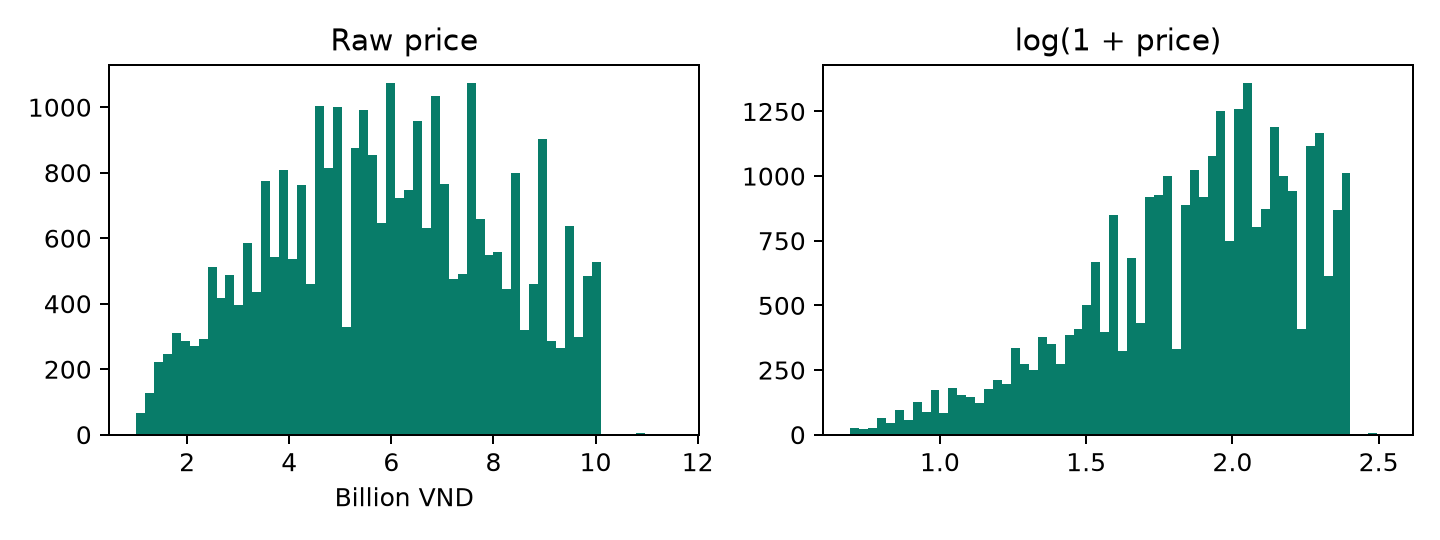
\includegraphics[width=\linewidth,height=.56\textheight,keepaspectratio]{media/media/image3.png}
\caption{Phân phối giá nhà trước và sau biến đổi logarit}\label{fig:legacy-2.1}
\end{figure}



\subsection{Định nghĩa mẫu, nhãn và đơn vị sử dụng}\label{ux111ux1ecbnh-nghux129a-mux1eabu-nhuxe3n-vuxe0-ux111ux1a1n-vux1ecb-sux1eed-dux1ee5ng}

Ở bài toán phân loại, một mẫu là một dòng dữ liệu và đầu ra là một trong
ba nhãn High, Moderate hoặc Low do dataset cung cấp. Chỉ tám biến số
được sử dụng nhằm tạo một đầu vào có thể kiểm soát trên giao diện. Việc
bỏ các biến chứa điểm nguy cơ hoặc khuyến nghị giúp tránh để mô hình học
lại một thông tin đã quá gần nhãn. Đây là lựa chọn chống rò rỉ ở cấp ngữ
nghĩa, khác với việc xóa cột vì hệ số tương quan cao.

\Needspace{7\baselineskip}
\captionof{table}{Từ điển đầu vào classifier và giá trị thiếu thực tế}\label{tab:legacy-2.3}

{\def\LTcaptype{none} % do not increment counter
\begin{longtable}[]{@{}
  >{\raggedright\arraybackslash}p{(\linewidth - 4\tabcolsep) * \real{0.3374}}
  >{\centering\arraybackslash}p{(\linewidth - 4\tabcolsep) * \real{0.4375}}
  >{\centering\arraybackslash}p{(\linewidth - 4\tabcolsep) * \real{0.2250}}@{}}
\toprule\noalign{}
\begin{minipage}[b]{\linewidth}\raggedright
\textbf{Biến}
\end{minipage} & \begin{minipage}[b]{\linewidth}\centering
\textbf{Ý nghĩa / đơn vị}
\end{minipage} & \begin{minipage}[b]{\linewidth}\raggedright
\textbf{Số thiếu trong 50.000 dòng}
\end{minipage} \\
\midrule\noalign{}
\endhead
\bottomrule\noalign{}
\endlastfoot
Age & Tuổi & 497 \\
BMI & Chỉ số khối cơ thể & 0 \\
HbA1c & Phần trăm & 1974 \\
Fasting\_Blood\_Sugar & Đường huyết lúc đói; mg/dL & 0 \\
Blood\_Glucose & Glucose; mg/dL & 959 \\
Blood\_Pressure\_Systolic & Huyết áp tâm thu; mmHg & 0 \\
HDL / LDL & mg/dL & 1.000 ở mỗi biến \\
\end{longtable}
}

\begin{figure}[H]
\centering
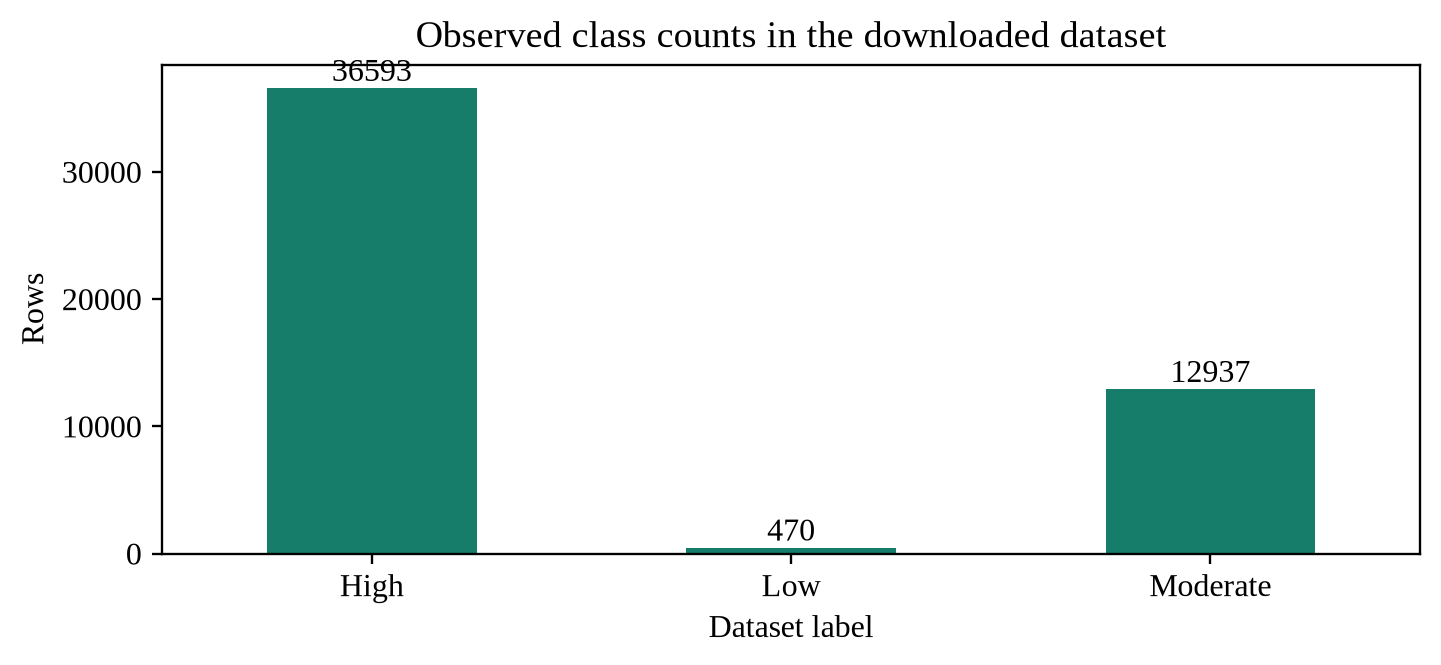
\includegraphics[width=\linewidth,height=.56\textheight,keepaspectratio]{media/media/image4.png}
\caption{Số lượng ba nhãn đếm trực tiếp từ tệp dữ liệu tải về}\label{fig:legacy-2.2}
\end{figure}



Nếu dự đoán mọi mẫu đều là High, Accuracy sẽ gần tỷ lệ của lớp lớn nhất
nhưng hệ thống không nhận diện được hai lớp còn lại. Bởi vậy phép so
sánh dùng macro-F1, cho mỗi lớp trọng số bằng nhau.
class\_weight=balanced tăng đóng góp của lớp hiếm trong quá trình học;
nó không tự biến điểm số của Random Forest thành xác suất nguy cơ lâm
sàng đã được hiệu chỉnh.

\subsection{Dữ liệu nhà ở và ý nghĩa của phép chia theo địa chỉ}\label{dux1eef-liux1ec7u-nhuxe0-ux1edf-vuxe0-uxfd-nghux129a-cux1ee7a-phuxe9p-chia-theo-ux111ux1ecba-chux1ec9}

Một mẫu nhà ở là một tin đăng với giá rao bán, không phải biên bản giao
dịch. Nhãn Price được giữ ở đơn vị tỷ VND. Các biến diện tích, mặt tiền,
đường vào, tầng, phòng và nhóm thông tin pháp lý/nội thất mô tả một phần
tài sản; biến Province chỉ lấy thành phần cuối của chuỗi địa chỉ. Cách
trích này đơn giản và tái lập được, nhưng chưa phải chuẩn hóa địa giới
hay mã hóa tọa độ địa lý.

Nhiều tin có thể cùng địa chỉ. Nếu chia theo dòng, mô hình có thể thấy
những bản ghi rất gần nhau trong cả train lẫn test. Project chuẩn hóa
địa chỉ bằng chữ thường và bỏ khoảng trắng hai đầu, rồi dùng địa chỉ làm
nhóm cho phép chia và GroupKFold. Kiểm tra sau chia cho kết quả 0 nhóm
chung ở cả ba cặp train--validation, train--test và validation--test.
Điều này giảm một nguồn rò rỉ, nhưng chưa phát hiện được hai cách viết
khác nhau của cùng địa chỉ.

\Needspace{7\baselineskip}
\captionof{table}{Đối chiếu số dòng và số nhóm sau chia dữ liệu nhà ở}\label{tab:legacy-2.4}

{\def\LTcaptype{none} % do not increment counter
\begin{longtable}[]{@{}
  >{\raggedright\arraybackslash}p{(\linewidth - 4\tabcolsep) * \real{0.3125}}
  >{\centering\arraybackslash}p{(\linewidth - 4\tabcolsep) * \real{0.3125}}
  >{\centering\arraybackslash}p{(\linewidth - 4\tabcolsep) * \real{0.3750}}@{}}
\toprule\noalign{}
\begin{minipage}[b]{\linewidth}\raggedright
\textbf{Tập}
\end{minipage} & \begin{minipage}[b]{\linewidth}\centering
\textbf{Số dòng}
\end{minipage} & \begin{minipage}[b]{\linewidth}\centering
\textbf{Số nhóm địa chỉ}
\end{minipage} \\
\midrule\noalign{}
\endhead
\bottomrule\noalign{}
\endlastfoot
train & 19377 & 6560 \\
validation & 4491 & 1640 \\
test & 6361 & 2051 \\
\end{longtable}
}

Mặt tiền thiếu khoảng 38,3\%, đường vào 44,0\%, hướng nhà 70,3\% và
hướng ban công 82,6\%. Điền trung vị cho biến số giữ được mẫu nhưng
không khôi phục thông tin thật đã mất. Giá trị Unknown của biến phân
loại cũng không đồng nghĩa một đặc điểm có thật của căn nhà. Vì vậy báo
cáo xem missingness là giới hạn dữ liệu, không chỉ là một thao tác kỹ
thuật trước huấn luyện.

\subsection{Pipeline và kiểm soát thông tin giữa các tập}\label{pipeline-vuxe0-kiux1ec3m-souxe1t-thuxf4ng-tin-giux1eefa-cuxe1c-tux1eadp}

\begin{figure}[H]
\centering
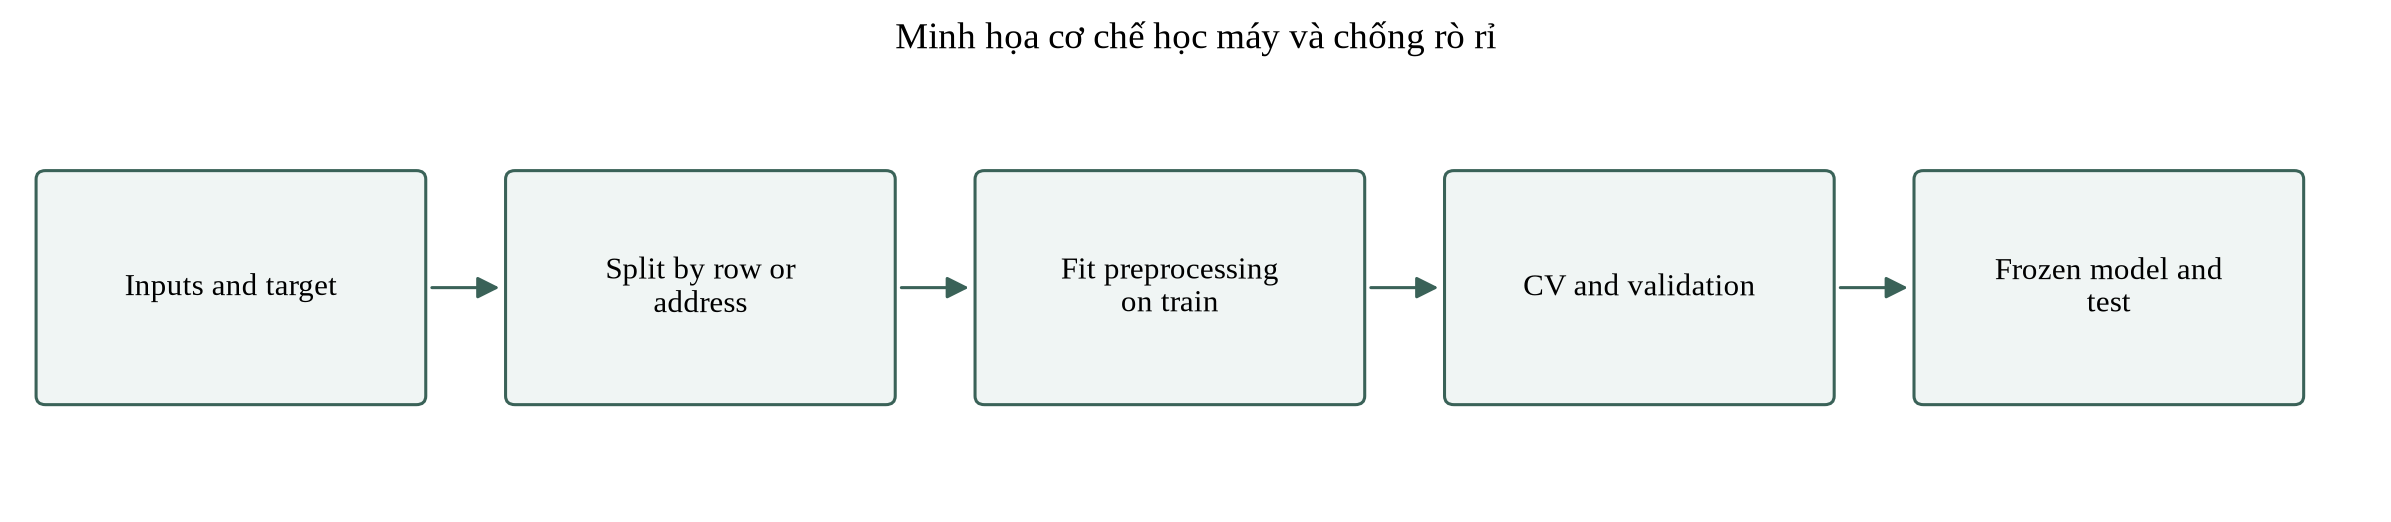
\includegraphics[width=\linewidth,height=.56\textheight,keepaspectratio]{media/media/image5.png}
\caption{Minh họa quy trình học máy; tiền xử lý chỉ được fit trên train}\label{fig:legacy-2.3}
\end{figure}



Trong mỗi fold, imputer tính trung vị từ phần train của fold; bộ chuẩn
hóa tính trung bình và độ lệch chuẩn ở cùng phạm vi; one-hot encoder chỉ
xây danh sách nhóm từ phần đó. Khi chuyển sang validation của fold, các
tham số này được giữ nguyên. Sau khi chọn cấu hình, mô hình cuối được
fit trên train, còn validation và test vẫn chỉ đi qua transform và
predict. Việc đóng gói các bước trong Pipeline giúp quy tắc này được
thực thi thống nhất thay vì phụ thuộc thao tác thủ công.

Random Forest không bắt buộc chuẩn hóa thang đo số, nhưng pipeline nhà ở
vẫn chuẩn hóa để các ứng viên Ridge và mô hình cây dùng cùng định nghĩa
tiền xử lý. log1p làm giảm mức chi phối của giá lớn trong quá trình học;
expm1 đưa dự đoán về tỷ VND trước đánh giá. Tối ưu sai số trên thang log
không đồng nghĩa tối ưu MAE trên thang giá, nên bước so sánh CV vẫn tính
theo đơn vị gốc.

\section{So sánh và lựa chọn mô hình}\label{so-suxe1nh-vuxe0-lux1ef1a-chux1ecdn-muxf4-huxecnh}

\Needspace{7\baselineskip}
\captionof{table}{So sánh phân loại với StratifiedKFold 3 phần}\label{tab:legacy-2.5}

{\def\LTcaptype{none} % do not increment counter
\begin{longtable}[]{@{}
  >{\raggedright\arraybackslash}p{(\linewidth - 2\tabcolsep) * \real{0.6250}}
  >{\centering\arraybackslash}p{(\linewidth - 2\tabcolsep) * \real{0.3750}}@{}}
\toprule\noalign{}
\begin{minipage}[b]{\linewidth}\raggedright
\textbf{Mô hình}
\end{minipage} & \begin{minipage}[b]{\linewidth}\centering
\textbf{CV macro-F1}
\end{minipage} \\
\midrule\noalign{}
\endhead
\bottomrule\noalign{}
\endlastfoot
Majority & 0.2817 \\
Logistic Regression & 0.5027 \\
KNN & 0.5055 \\
Decision Tree & 0.5610 \\
Random Forest & 0.6203 \\
SVM RBF & 0.5729 \\
\end{longtable}
}

Random Forest được chọn bằng CV macro-F1 0.6203, gồm 80 cây,
max\_depth=10, class\_weight=balanced, random\_state=42. Macro-F1 train
0.7105, validation 0.6059 và test 0.6087 cho thấy vẫn có khoảng cách
khái quát hóa. Không dùng test để tăng độ sâu cây.

\Needspace{7\baselineskip}
\captionof{table}{So sánh hồi quy với GroupKFold 3 phần}\label{tab:legacy-2.6}

{\def\LTcaptype{none} % do not increment counter
\begin{longtable}[]{@{}
  >{\raggedright\arraybackslash}p{(\linewidth - 2\tabcolsep) * \real{0.6250}}
  >{\centering\arraybackslash}p{(\linewidth - 2\tabcolsep) * \real{0.3750}}@{}}
\toprule\noalign{}
\begin{minipage}[b]{\linewidth}\raggedright
\textbf{Mô hình}
\end{minipage} & \begin{minipage}[b]{\linewidth}\centering
\textbf{CV MAE (tỷ VND)}
\end{minipage} \\
\midrule\noalign{}
\endhead
\bottomrule\noalign{}
\endlastfoot
Median & 1.8623 \\
Log Ridge & 1.4915 \\
Log Random Forest & 1.3091 \\
Log Gradient Boosting & 1.3246 \\
\end{longtable}
}

Hồi quy chọn Log Random Forest với 80 cây, max\_depth=14,
min\_samples\_leaf=3. Ridge thử alpha 1, 10, 100; Gradient Boosting thử
learning\_rate 0,04 và 0,08. Tất cả cấu hình cùng một nhóm train và các
fold theo địa chỉ. Mô hình trung vị cung cấp mốc đánh giá độ hữu ích của
các mô hình học được.

\section{Kết quả test độc lập và phân tích sai số}\label{kux1ebft-quux1ea3-test-ux111ux1ed9c-lux1eadp-vuxe0-phuxe2n-tuxedch-sai-sux1ed1}

\Needspace{7\baselineskip}
\captionof{table}{Kết quả được tính từ predictions của main.ipynb}\label{tab:legacy-2.7}

{\def\LTcaptype{none} % do not increment counter
\begin{longtable}[]{@{}
  >{\raggedright\arraybackslash}p{(\linewidth - 4\tabcolsep) * \real{0.2500}}
  >{\raggedright\arraybackslash}p{(\linewidth - 4\tabcolsep) * \real{0.3750}}
  >{\centering\arraybackslash}p{(\linewidth - 4\tabcolsep) * \real{0.3750}}@{}}
\toprule\noalign{}
\begin{minipage}[b]{\linewidth}\raggedright
\textbf{Bài toán}
\end{minipage} & \begin{minipage}[b]{\linewidth}\centering
\textbf{Chỉ số}
\end{minipage} & \begin{minipage}[b]{\linewidth}\centering
\textbf{Kết quả}
\end{minipage} \\
\midrule\noalign{}
\endhead
\bottomrule\noalign{}
\endlastfoot
Phân loại nguy cơ & Accuracy / Precision macro & 0.7788 / 0.5708 \\
Phân loại nguy cơ & Recall macro / F1 macro & 0.7231 / 0.6087 \\
Giá nhà & MAE / RMSE (tỷ VND) & 1.2760 / 1.6394 \\
Giá nhà & MSE / R2 & 2.6877 / 0.4273 \\
\end{longtable}
}

\begin{figure}[H]
\centering
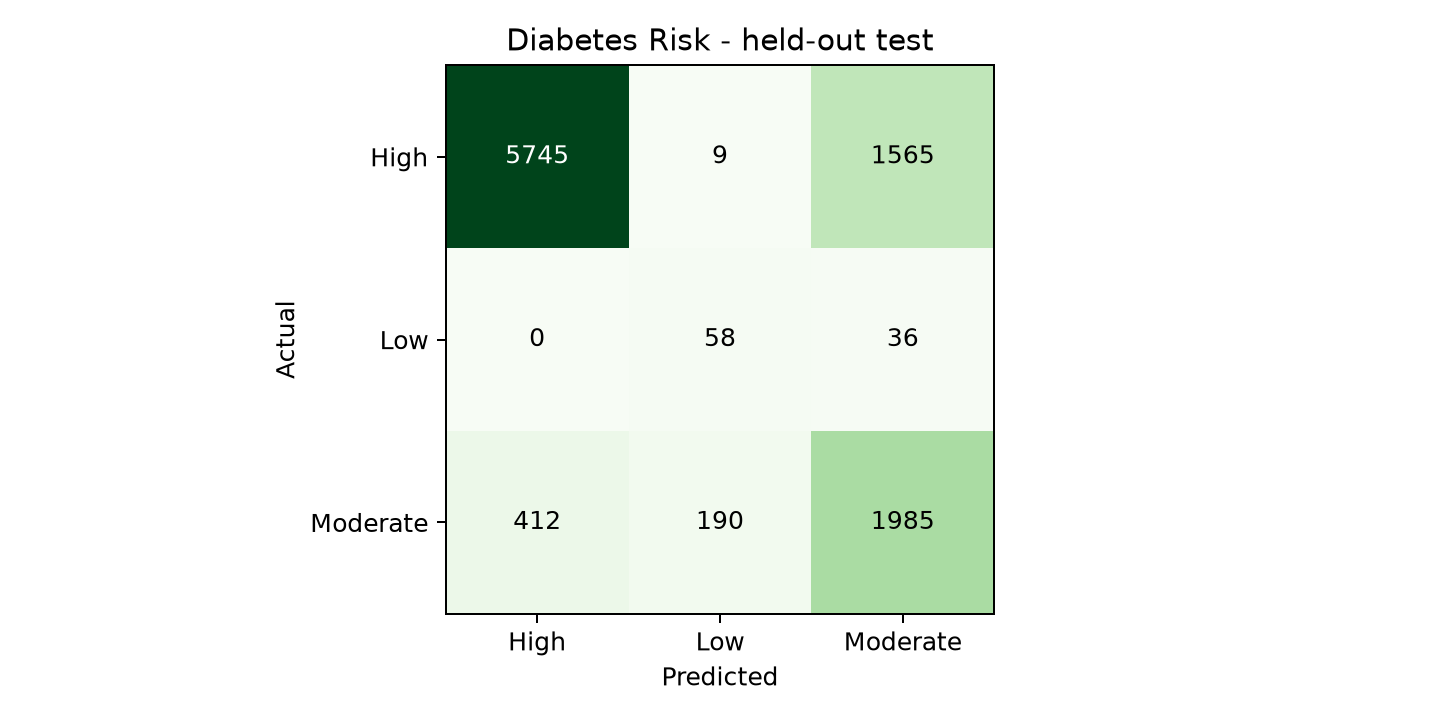
\includegraphics[width=\linewidth,height=.56\textheight,keepaspectratio]{media/media/image6.png}
\caption{Ma trận nhầm lẫn của phân loại nguy cơ trên 10.000 mẫu test}\label{fig:legacy-2.4}
\end{figure}



Ma trận nhầm lẫn cho thấy Accuracy chịu ảnh hưởng lớn của lớp High.
Macro-precision thấp hơn macro-recall phản ánh chi phí dự đoán nhầm khi
dùng class\_weight=balanced. Nhãn dự đoán chỉ mô tả quy tắc của dataset,
không phải chẩn đoán hoặc nguy cơ bệnh ngoài đời.

\begin{figure}[H]
\centering
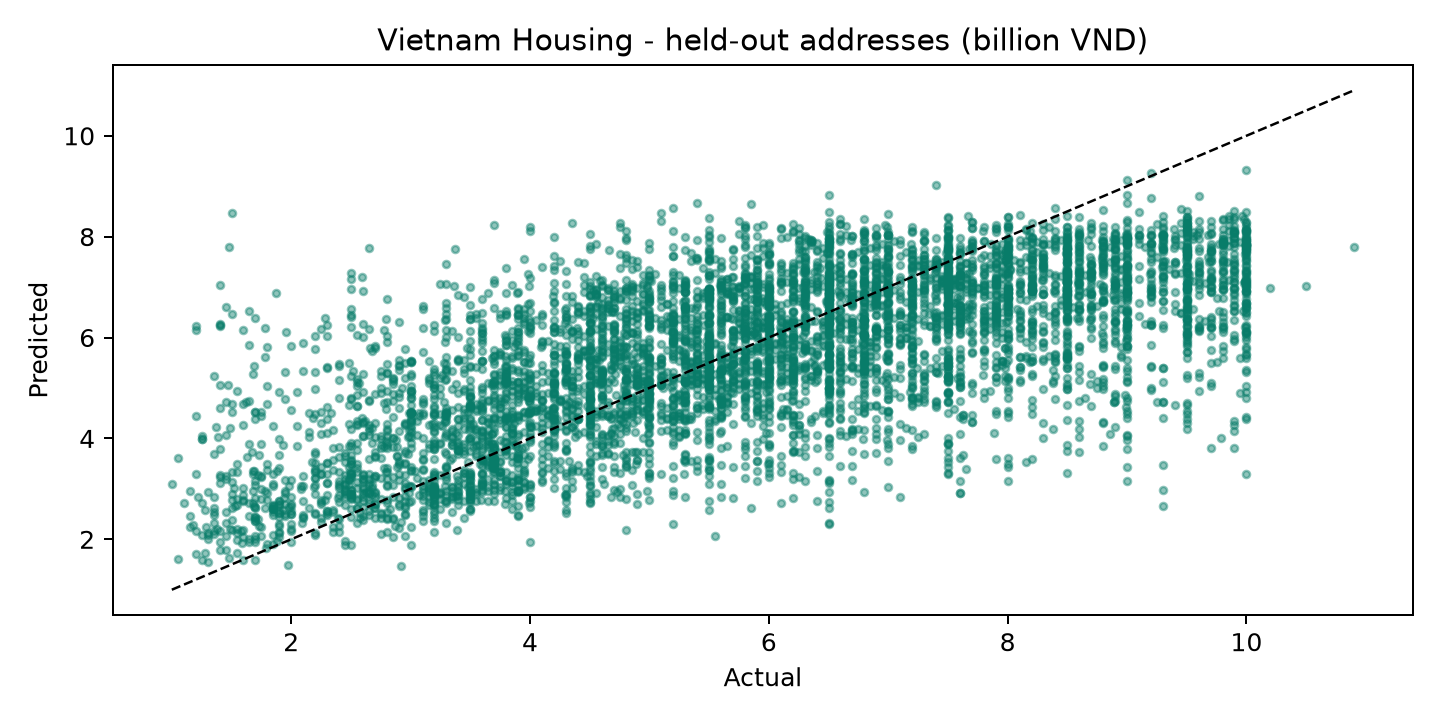
\includegraphics[width=\linewidth,height=.56\textheight,keepaspectratio]{media/media/image7.png}
\caption{Giá nhà dự đoán và thực tế tại các địa chỉ giữ riêng}\label{fig:legacy-2.5}
\end{figure}



MAE train của giá nhà là 1.0276 tỷ VND, validation 1.2936, test 1.2760;
R2 test 0.4273. Sai số tuyệt đối còn lớn đối với định giá cá nhân. Các
thông tin vị trí trong địa chỉ, chất lượng tin đăng và thời điểm giao
dịch chưa được mô hình hóa đầy đủ. Mức lệch giữa train và test cần được
theo dõi trước khi tăng độ phức tạp.

\subsection{Hiệu năng từng lớp và tác động của mất cân bằng}\label{hiux1ec7u-nux103ng-tux1eebng-lux1edbp-vuxe0-tuxe1c-ux111ux1ed9ng-cux1ee7a-mux1ea5t-cuxe2n-bux1eb1ng}

\Needspace{7\baselineskip}
\captionof{table}{Chỉ số từng lớp tính lại từ diabetes\_predictions.csv}\label{tab:legacy-2.8}

{\def\LTcaptype{none} % do not increment counter
\begin{longtable}[]{@{}
  >{\raggedright\arraybackslash}p{(\linewidth - 8\tabcolsep) * \real{0.2000}}
  >{\centering\arraybackslash}p{(\linewidth - 8\tabcolsep) * \real{0.2000}}
  >{\centering\arraybackslash}p{(\linewidth - 8\tabcolsep) * \real{0.2000}}
  >{\centering\arraybackslash}p{(\linewidth - 8\tabcolsep) * \real{0.2000}}
  >{\centering\arraybackslash}p{(\linewidth - 8\tabcolsep) * \real{0.2000}}@{}}
\toprule\noalign{}
\begin{minipage}[b]{\linewidth}\raggedright
\textbf{Lớp}
\end{minipage} & \begin{minipage}[b]{\linewidth}\centering
\textbf{Precision}
\end{minipage} & \begin{minipage}[b]{\linewidth}\centering
\textbf{Recall}
\end{minipage} & \begin{minipage}[b]{\linewidth}\centering
\textbf{F1}
\end{minipage} & \begin{minipage}[b]{\linewidth}\centering
\textbf{Mẫu test}
\end{minipage} \\
\midrule\noalign{}
\endhead
\bottomrule\noalign{}
\endlastfoot
High & 0.9331 & 0.7849 & 0.8526 & 7319 \\
Low & 0.2257 & 0.6170 & 0.3305 & 94 \\
Moderate & 0.5535 & 0.7673 & 0.6431 & 2587 \\
\end{longtable}
}

Lớp Low chỉ có 94 mẫu test. Recall 0,6170 nghĩa là mô hình tìm được
khoảng 61,7\% số mẫu Low thực tế, trong khi precision 0,2257 cho thấy
nhiều dự đoán Low là nhầm từ lớp khác. Với High, precision 0,9331 cao
hơn nhưng recall chỉ 0,7849. Nhìn riêng Accuracy 0,7788 sẽ che bớt sự
khác nhau này. Kết quả phù hợp với tác động của cân bằng trọng số: tăng
khả năng nhận diện lớp ít mẫu nhưng có thể tăng số dương tính giả theo
cách xét từng lớp.

Chưa có tập bệnh nhân bên ngoài, nhãn lâm sàng độc lập hoặc đánh giá
hiệu chỉnh xác suất. Do đó giao diện chỉ hiển thị nhãn dataset và giải
thích phạm vi, không chuyển High thành chẩn đoán mắc bệnh, không đưa
phần trăm nguy cơ cá nhân và không gắn khuyến nghị điều trị với đầu ra.
Hướng cải tiến có cơ sở là xây dữ liệu xác minh và kiểm tra khả năng
chuyển miền trước khi tăng số cây hoặc thêm một mạng sâu.

\subsection{Sai số nhà ở theo phân khúc và phần dư}\label{sai-sux1ed1-nhuxe0-ux1edf-theo-phuxe2n-khuxfac-vuxe0-phux1ea7n-dux1b0}

\begin{figure}[H]
\centering
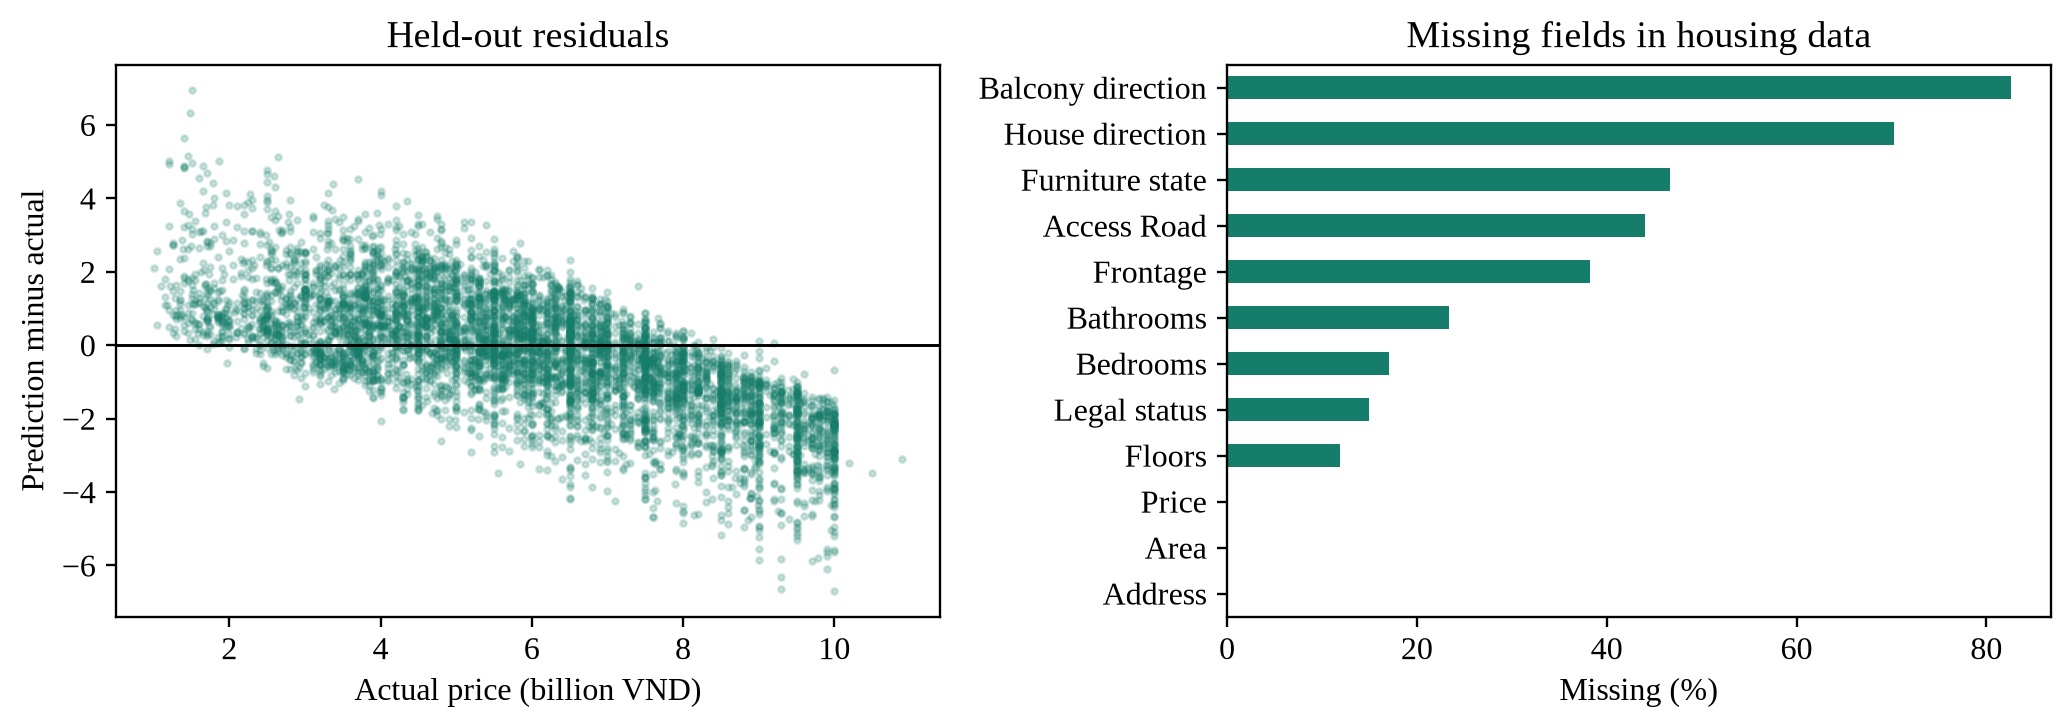
\includegraphics[width=\linewidth,height=.56\textheight,keepaspectratio]{media/media/image8.png}
\caption{Phần dư test và tỷ lệ thiếu của dữ liệu nhà ở}\label{fig:legacy-2.6}
\end{figure}



\Needspace{7\baselineskip}
\captionof{table}{Phân tích test theo bốn nhóm lượng tử của giá thực}\label{tab:legacy-2.9}

{\def\LTcaptype{none} % do not increment counter
\begin{longtable}[]{@{}
  >{\raggedright\arraybackslash}p{(\linewidth - 6\tabcolsep) * \real{0.3750}}
  >{\centering\arraybackslash}p{(\linewidth - 6\tabcolsep) * \real{0.1562}}
  >{\centering\arraybackslash}p{(\linewidth - 6\tabcolsep) * \real{0.2313}}
  >{\centering\arraybackslash}p{(\linewidth - 6\tabcolsep) * \real{0.2375}}@{}}
\toprule\noalign{}
\begin{minipage}[b]{\linewidth}\raggedright
\textbf{Khoảng giá thực (tỷ)}
\end{minipage} & \begin{minipage}[b]{\linewidth}\centering
\textbf{Mẫu}
\end{minipage} & \begin{minipage}[b]{\linewidth}\centering
\textbf{MAE (tỷ)}
\end{minipage} & \begin{minipage}[b]{\linewidth}\centering
\textbf{Lệch TB (tỷ)}
\end{minipage} \\
\midrule\noalign{}
\endhead
\bottomrule\noalign{}
\endlastfoot
(0.999, 4.3{]} & 1607 & 1.197 & +0.988 \\
(4.3, 5.95{]} & 1594 & 0.995 & +0.420 \\
(5.95, 7.56{]} & 1570 & 0.967 & -0.470 \\
(7.56, 10.9{]} & 1590 & 1.943 & -1.932 \\
\end{longtable}
}

Phần dư được định nghĩa bằng dự đoán trừ giá thực. Nhóm giá thấp có lệch
trung bình dương, còn nhóm trên 7,56 tỷ có lệch khoảng −1,932 tỷ và MAE
khoảng 1,943 tỷ. Mẫu hình này cho thấy dự đoán có xu hướng co về vùng
trung tâm: nhà rẻ bị định giá cao, nhà đắt bị định giá thấp. Đây là mô
tả từ test đã khóa, không phải căn cứ để sửa dự đoán theo chính giá thực
của từng mẫu.

Trung vị sai số tuyệt đối là 1.038 tỷ VND; phân vị 90\% là 2.688 tỷ VND.
Hai đại lượng mô tả phân phối lỗi của tập test, không phải khoảng dự báo
90\% cho một căn nhà mới. Để có khoảng dự báo cá nhân cần một quy trình
hiệu chỉnh riêng và kiểm tra độ bao phủ ngoài mẫu.

\subsection{Hai tình huống sử dụng trên web}\label{hai-tuxecnh-huux1ed1ng-sux1eed-dux1ee5ng-truxean-web}

Với giá nhà, người dùng nhập sáu biến số và chọn năm nhóm thuộc tính.
Giá trị số trống được điền bằng trung vị train và API trả cảnh báo; nhóm
chưa gặp được mã hóa thành vector 0 của nhóm tương ứng và cũng được cảnh
báo. Phiên bản hoàn thiện dùng nhóm phổ biến nhất của train làm mặc định
thay vì mục đầu danh sách chữ cái. Các giá trị mặc định tạo một kịch bản
nhập liệu, không được giới thiệu là một tài sản quan sát thực tế.

Sau khi nhấn Chạy mô hình, API kiểm tra kiểu và tính hữu hạn, biến đổi
đặc trưng bằng tham số train, chạy các cây đã xuất và trả giá theo tỷ
VND. Một giá trị vượt min--max train không bị tự cắt về biên; hệ thống
giữ đầu vào và đánh dấu ngoài phạm vi. Kết quả phù hợp để quan sát mô
hình và đối chiếu kịch bản, chưa đủ cho quyết định mua bán.

\productlink{Truy cập sản phẩm thực nghiệm}{https://rag-httm-chatbot.vercel.app/?demo=housing\#experiments}

Với classifier, giao diện yêu cầu đúng đơn vị đã ghi trong từ điển đầu
vào. Giá trị thiếu được xử lý giống quy trình train; sai kiểu, số không
hữu hạn hoặc giá trị không dương bị từ chối. Điểm theo lớp của rừng cây
là kết quả tổng hợp của mô hình trên nhãn tổng hợp. Vì chưa hiệu chỉnh
và chưa xác minh lâm sàng, phần hiển thị ưu tiên nhãn cùng cảnh báo thay
vì đặt tên điểm số là xác suất mắc bệnh.

\productlink{Truy cập sản phẩm thực nghiệm}{https://rag-httm-chatbot.vercel.app/?demo=diabetes_classifier\#experiments}

\section{Kết luận chương}\label{kux1ebft-luux1eadn-chux1b0ux1a1ng}

Với dữ liệu dạng bảng, Random Forest và Gradient Boosting thường cạnh
tranh tốt với Deep Learning. Không có một mô hình đơn lẻ phù hợp với mọi
tập dữ liệu.

Hai bài toán cho thấy điểm số phụ thuộc cách xác định nhãn, phép chia dữ
liệu và thước đo. Macro-F1 giúp nhận rõ hạn chế ở lớp hiếm; chia theo
địa chỉ giúp đánh giá giá nhà ngoài các nhóm đã gặp. Dù Random Forest
được chọn trong cả hai bài toán, chất lượng đầu vào và miền sử dụng vẫn
là giới hạn chính. Các tệp checkpoint, dự đoán và bảng CV được giữ để có
thể kiểm tra lại từng kết luận.

\chapter{Mạng nơ-ron tích chập CNN}\label{chux1b0ux1a1ng-3.-mux1ea1ng-nux1a1-ron-tuxedch-chux1eadp-CNN}

Một chữ số viết tay có thể xuất hiện ở nhiều vị trí và có độ đậm, độ
nghiêng khác nhau. Nếu coi mỗi pixel là một thuộc tính độc lập, mô hình
phải học lại nhiều quan hệ giống nhau ở các vùng ảnh khác nhau. Bài toán
của chương là nhận dạng chữ số đồng thời khai thác được cấu trúc không
gian cục bộ của ảnh.

CNN giải quyết vấn đề bằng kernel dùng chung, các phép biến đổi phi
tuyến và giảm kích thước không gian. Mạng được huấn luyện từ đầu trên
MNIST để có thể theo dõi đầy đủ từ ảnh gốc đến trọng số, feature map và
đầu ra. Mục tiêu không chỉ là đạt Accuracy cao mà còn kiểm tra xem phép
tích chập trong mã có đúng với cơ chế đã giải thích và mô hình sai ở
những trường hợp nào.

Chương đi từ cấu trúc tầng đến lan truyền gradient, xây kiến trúc cụ
thể, đánh giá trên 10.000 ảnh test và đưa mô hình lên web. Sự khác nhau
giữa ảnh test chuẩn và ảnh người dùng vẽ trực tiếp được xem là một giới
hạn của triển khai, không được bỏ qua khi diễn giải kết quả.

\section{Lý thuyết CNN}\label{luxfd-thuyux1ebft-CNN}

\subsection{Tại sao cần CNN?}\label{tux1ea1i-sao-cux1ea7n-CNN}

Với ảnh 224×224×3 (RGB), nếu dùng Dense layer thông thường:

\begin{quote}
• Số tham số đầu vào: 224 × 224 × 3 = 150,528 giá trị

• Một Dense layer với 1000 nơ-ron: 150 triệu tham số --- bùng nổ tham
số!
\end{quote}

CNN giải quyết bằng 3 ý tưởng chính:

1. Local connectivity: Mỗi nơ-ron chỉ nhìn một vùng nhỏ của ảnh

2. Weight sharing: Cùng một kernel dùng chung cho toàn bộ ảnh

3. Translation equivariance: phép tích chập dùng chung kernel khi dịch
đầu vào; pooling tạo bất biến cục bộ ở mức độ nhất định.

\subsection{Phép Tích chập (Convolution)}\label{phuxe9p-tuxedch-chux1eadp-convolution}

Với kernel K kích thước (kH × kW) và ảnh đầu vào X kích thước (H × W):

\(Z(i,j) = \sum_{u = 0}^{k_{H} - 1}{\sum_{v = 0}^{k_{W} - 1}X}(i + u,j + v)K(u,v) + b\)
(3.1)

Kích thước đầu ra (với padding P, stride S):

\(H_{out} = \left\lfloor \frac{H - k_{H} + 2P}{S} \right\rfloor + 1\)
(3.2)

\subsection{Pooling}\label{pooling}

Max Pooling: Lấy giá trị lớn nhất trong mỗi vùng → giảm kích thước, giữ
đặc trưng nổi bật

\(P_{\max}(i,j) = \max_{(u,v) \in R_{ij}}Z(u,v)\) (3.3)

Average Pooling: Lấy trung bình → giảm kích thước mượt hơn

\subsection{Kiến trúc CNN điển hình}\label{kiux1ebfn-truxfac-CNN-ux111iux1ec3n-huxecnh}

Input → {[}Conv → BN → ReLU → MaxPool{]} × N → Flatten → Dense → Softmax

\Needspace{7\baselineskip}
\captionof{table}{Vai trò của các tầng CNN}\label{tab:legacy-3.1}

{\def\LTcaptype{none} % do not increment counter
\begin{longtable}[]{@{}
  >{\raggedright\arraybackslash}p{(\linewidth - 2\tabcolsep) * \real{0.2500}}
  >{\raggedright\arraybackslash}p{(\linewidth - 2\tabcolsep) * \real{0.7500}}@{}}
\toprule\noalign{}
\begin{minipage}[b]{\linewidth}\raggedright
\textbf{Tầng}
\end{minipage} & \begin{minipage}[b]{\linewidth}\centering
\textbf{Vai trò}
\end{minipage} \\
\midrule\noalign{}
\endhead
\bottomrule\noalign{}
\endlastfoot
Conv2D & Trích xuất đặc trưng cục bộ: cạnh, góc, texture \\
BatchNorm & Chuẩn hóa giúp huấn luyện ổn định hơn \\
ReLU & Tạo tính phi tuyến \\
MaxPool & Giảm kích thước, tăng receptive field \\
Dropout & Điều chuẩn, hạn chế quá khớp \\
Dense và Softmax & Phân loại đa lớp \\
\end{longtable}
}

\subsection{Các kiến trúc CNN tiêu biểu}\label{cuxe1c-kiux1ebfn-truxfac-CNN-tiuxeau-biux1ec3u}

\Needspace{7\baselineskip}
\captionof{table}{Các kiến trúc CNN và đặc trưng thiết kế đã hiệu chỉnh}\label{tab:legacy-3.2}

{\def\LTcaptype{none} % do not increment counter
\begin{longtable}[]{@{}
  >{\raggedright\arraybackslash}p{(\linewidth - 4\tabcolsep) * \real{0.2187}}
  >{\centering\arraybackslash}p{(\linewidth - 4\tabcolsep) * \real{0.1250}}
  >{\raggedright\arraybackslash}p{(\linewidth - 4\tabcolsep) * \real{0.6563}}@{}}
\toprule\noalign{}
\begin{minipage}[b]{\linewidth}\raggedright
\textbf{Kiến trúc}
\end{minipage} & \begin{minipage}[b]{\linewidth}\centering
\textbf{Năm}
\end{minipage} & \begin{minipage}[b]{\linewidth}\centering
\textbf{Đặc điểm}
\end{minipage} \\
\midrule\noalign{}
\endhead
\bottomrule\noalign{}
\endlastfoot
LeNet-5 & 1998 & Nhận dạng chữ số, convolution và subsampling \\
AlexNet & 2012 & ReLU, Dropout và huấn luyện GPU \\
VGG & 2014 & Các kernel 3 × 3 xếp chồng \\
GoogLeNet & 2014 & Các nhánh Inception \\
ResNet & 2015 & Kết nối residual \\
EfficientNet & 2019 & Compound scaling độ sâu, độ rộng và độ phân
giải \\
\end{longtable}
}

LeNet-5 (1998) hướng tới nhận dạng ký tự và chữ số; các kiến trúc về sau
mở rộng khả năng học biểu diễn trên ảnh phức tạp hơn. Chỉ số Top-5 của
các biến thể, dataset hoặc chế độ ensemble khác nhau không tạo thành một
phép so sánh thống nhất. Bảng 3.2 đối chiếu đặc điểm kiến trúc; các kết
quả định lượng của chương được tính riêng trên MNIST.

\subsection{Backpropagation, loss và optimizer}\label{backpropagation-loss-vuxe0-optimizer}

Lan truyền xuôi tạo logits của từng lớp; CrossEntropyLoss kết hợp
log-softmax và negative log likelihood, vì vậy không áp softmax trước
loss trong PyTorch. Backpropagation dùng quy tắc chuỗi để tính gradient
của kernel và dense layer. Adam cập nhật trọng số dựa trên các ước lượng
moment của gradient; learning rate, weight decay và checkpoint được lựa
chọn mà không nhìn test.

\(\frac{\partial\mathcal{L}}{\partial K_{uv}} = \sum_{i,j}^{}\frac{\partial\mathcal{L}}{\partial Y_{ij}}X_{i + u,j + v}\)
(3.4)

Trong (3.4), K là kernel, X là đầu vào và Y là đầu ra trước kích hoạt;
chỉ số u,v xác định phần tử kernel và i,j chạy qua vị trí đầu ra. Cùng
một trọng số được dùng tại nhiều vị trí nên gradient là tổng đóng góp ở
các vị trí đó.

\subsection{Transfer learning và data augmentation}\label{transfer-learning-vuxe0-data-augmentation}

Transfer learning khởi tạo từ mạng đã học trên tập lớn, thay đầu phân
loại rồi đóng băng hoặc fine-tune một số tầng. Nó hữu ích khi dữ liệu
đích ít nhưng phải công bố phần pretrained và phần được học lại. Thực
nghiệm MNIST dưới đây không dùng pretrained; augmentation chỉ dịch ảnh
train ±1 pixel, giữ nguyên validation và test. Không dùng phép xoay mạnh
làm thay đổi ý nghĩa giữa các chữ số.

\section{Dữ liệu ảnh và kiến trúc thực nghiệm}\label{dux1eef-liux1ec7u-ux1ea3nh-vuxe0-kiux1ebfn-truxfac-thux1ef1c-nghiux1ec7m}

MNIST có 60.000 ảnh train gốc và 10.000 ảnh test độc lập, ảnh xám 28 ×
28, nhãn 0--9. Tách 12.000 ảnh từ train làm validation theo
stratification, còn 48.000 ảnh huấn luyện. Mỗi pixel được chia 255;
không học thống kê từ test. Bộ tải đọc trực tiếp các tệp IDX nén gzip,
kiểm tra magic number, số lượng ảnh và kích thước.

\Needspace{7\baselineskip}
\captionof{table}{Kiến trúc CNN tự huấn luyện}\label{tab:legacy-3.3}

{\def\LTcaptype{none} % do not increment counter
\begin{longtable}[]{@{}
  >{\raggedright\arraybackslash}p{(\linewidth - 4\tabcolsep) * \real{0.3437}}
  >{\centering\arraybackslash}p{(\linewidth - 4\tabcolsep) * \real{0.2500}}
  >{\centering\arraybackslash}p{(\linewidth - 4\tabcolsep) * \real{0.4062}}@{}}
\toprule\noalign{}
\begin{minipage}[b]{\linewidth}\raggedright
\textbf{Tầng}
\end{minipage} & \begin{minipage}[b]{\linewidth}\centering
\textbf{Kích thước đầu ra}
\end{minipage} & \begin{minipage}[b]{\linewidth}\centering
\textbf{Tham số}
\end{minipage} \\
\midrule\noalign{}
\endhead
\bottomrule\noalign{}
\endlastfoot
Ảnh vào & 1 × 28 × 28 & Pixel / 255 \\
Conv1 + ReLU + MaxPool & 8 × 14 × 14 & Kernel 3; padding 1; pool 2 \\
Conv2 + ReLU + MaxPool & 16 × 7 × 7 & Kernel 3; padding 1; pool 2 \\
Flatten + Dense + ReLU & 64 & 784 → 64 \\
Dense logits & 10 & 64 → 10 \\
\end{longtable}
}

Mạng có 52,138 tham số, train từ đầu 8 epoch trên CPU, Adam
learning\_rate=0,001, batch\_size=128, weight\_decay=0,0001 và gradient
clipping norm=1. Checkpoint có validation loss nhỏ nhất nằm ở epoch 8.
Thời gian thực nghiệm ghi trong metadata là 93.5 giây trên môi trường
hiện tại.

\subsection{Theo dõi một phép tích chập từ ảnh và trọng số thật}\label{theo-duxf5i-mux1ed9t-phuxe9p-tuxedch-chux1eadp-tux1eeb-ux1ea3nh-vuxe0-trux1ecdng-sux1ed1-thux1eadt}

\begin{figure}[H]
\centering
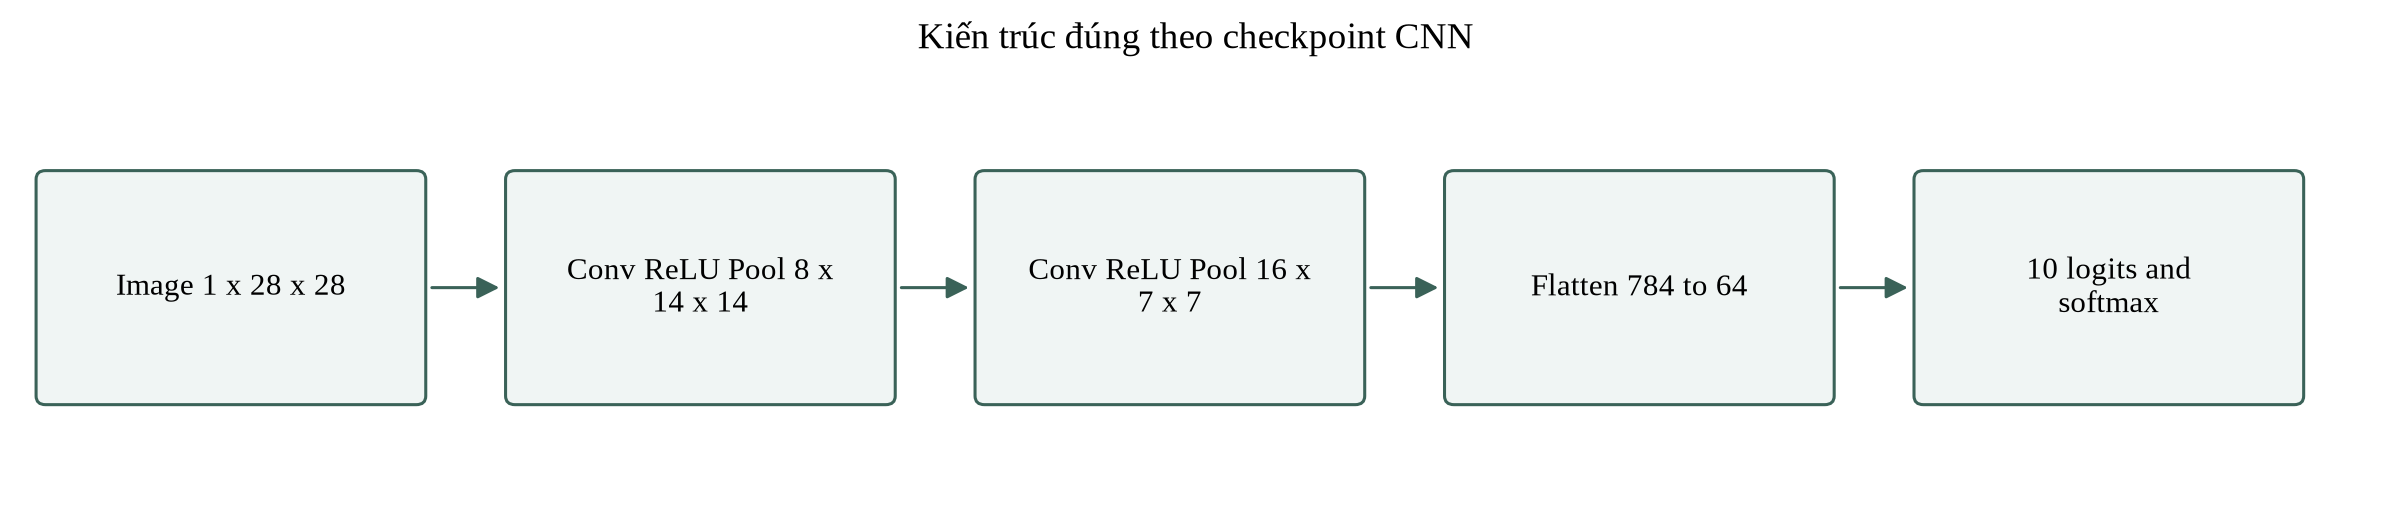
\includegraphics[width=\linewidth,height=.56\textheight,keepaspectratio]{media/media/image9.png}
\caption{Luồng tensor đúng với kiến trúc trong checkpoint}\label{fig:legacy-3.1}
\end{figure}



Mỗi kernel 3 × 3 được trượt qua ảnh và dùng lại cùng chín trọng số tại
mọi vị trí. Trong cài đặt Conv2d, phép toán là tương quan chéo: kernel
không bị đảo chiều như một số định nghĩa tích chập toán học. Padding 1
giữ chiều cao và chiều rộng; ReLU đặt giá trị âm về 0; max-pooling 2 × 2
chọn cực đại trên các ô không chồng lấn và giảm mỗi chiều xuống một nửa.

\begin{figure}[H]
\centering
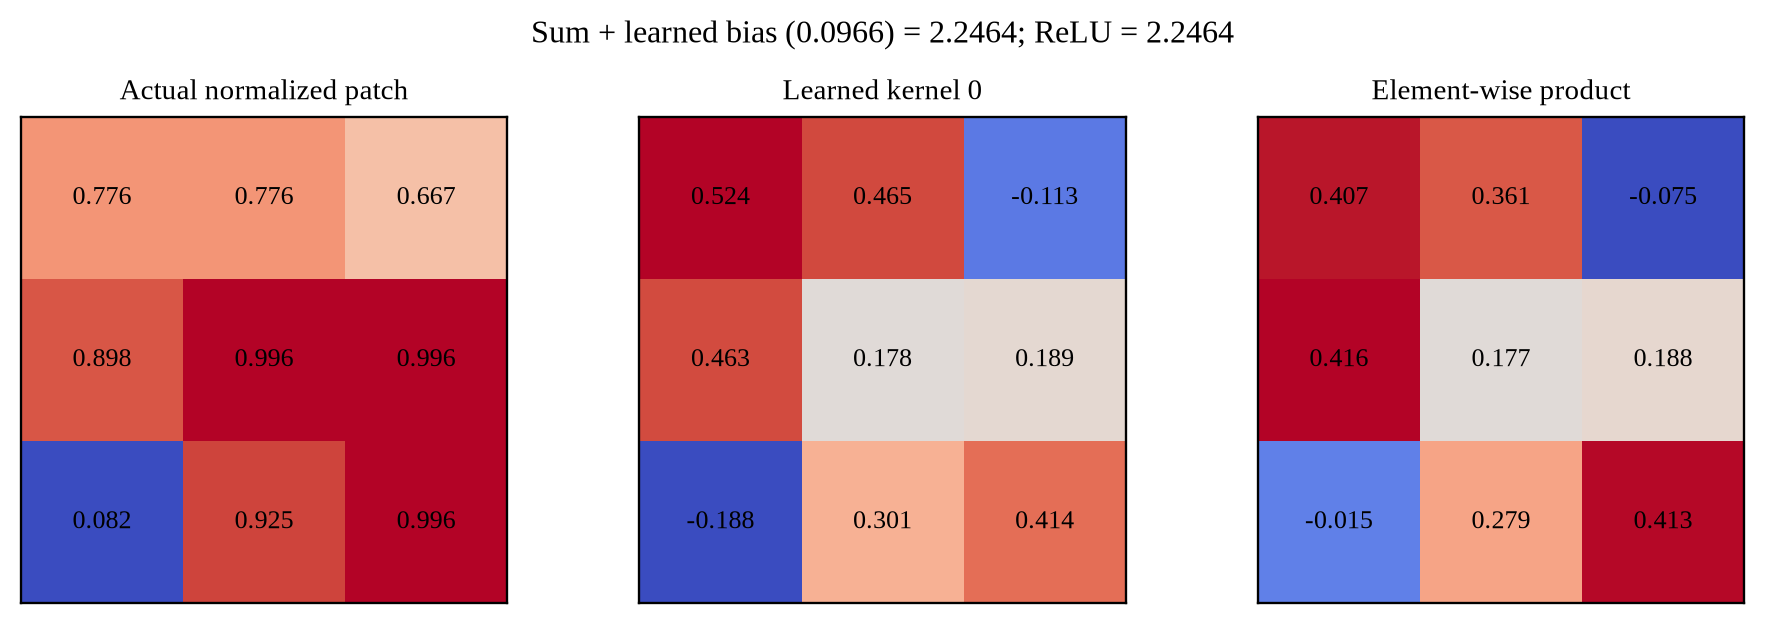
\includegraphics[width=\linewidth,height=.56\textheight,keepaspectratio]{media/media/image10.png}
\caption{Patch MNIST test{[}0{]}, kernel Conv1 kênh 0 và tích từng phần tử}\label{fig:legacy-3.2}
\end{figure}



Hình trên lấy ảnh đầu tiên của test, nhãn thật 7; chọn vị trí kích hoạt
lớn nhất của kênh 0 theo một quy tắc cố định. Với chỉ số bắt đầu từ 0,
hàng 9, cột 19, tổng chín tích cộng bias 0.096586 bằng 2.246353. Kết quả
ReLU đọc trực tiếp từ PyTorch là 2.246353. Sai khác nhỏ chỉ do phép tính
số thực, được assert nhỏ hơn 0,00001 trong mã phân tích.

Ví dụ này không dùng một ma trận số đặt sẵn để minh họa. Patch lấy từ
tệp IDX, kernel và bias lấy từ checkpoint, ảnh tích từng phần tử được
tạo bởi code. Do đó có thể lần ngược mỗi con số về đầu vào và tham số đã
học. Tuy nhiên, một activation lớn không tự chứng minh kênh đó biểu diễn
một khái niệm có tên như ``nét chéo''; đó chỉ là phản ứng số của kernel
trên ảnh đang xét.

\subsection{Feature map, receptive field và số tham số}\label{feature-map-receptive-field-vuxe0-sux1ed1-tham-sux1ed1}

\begin{figure}[H]
\centering
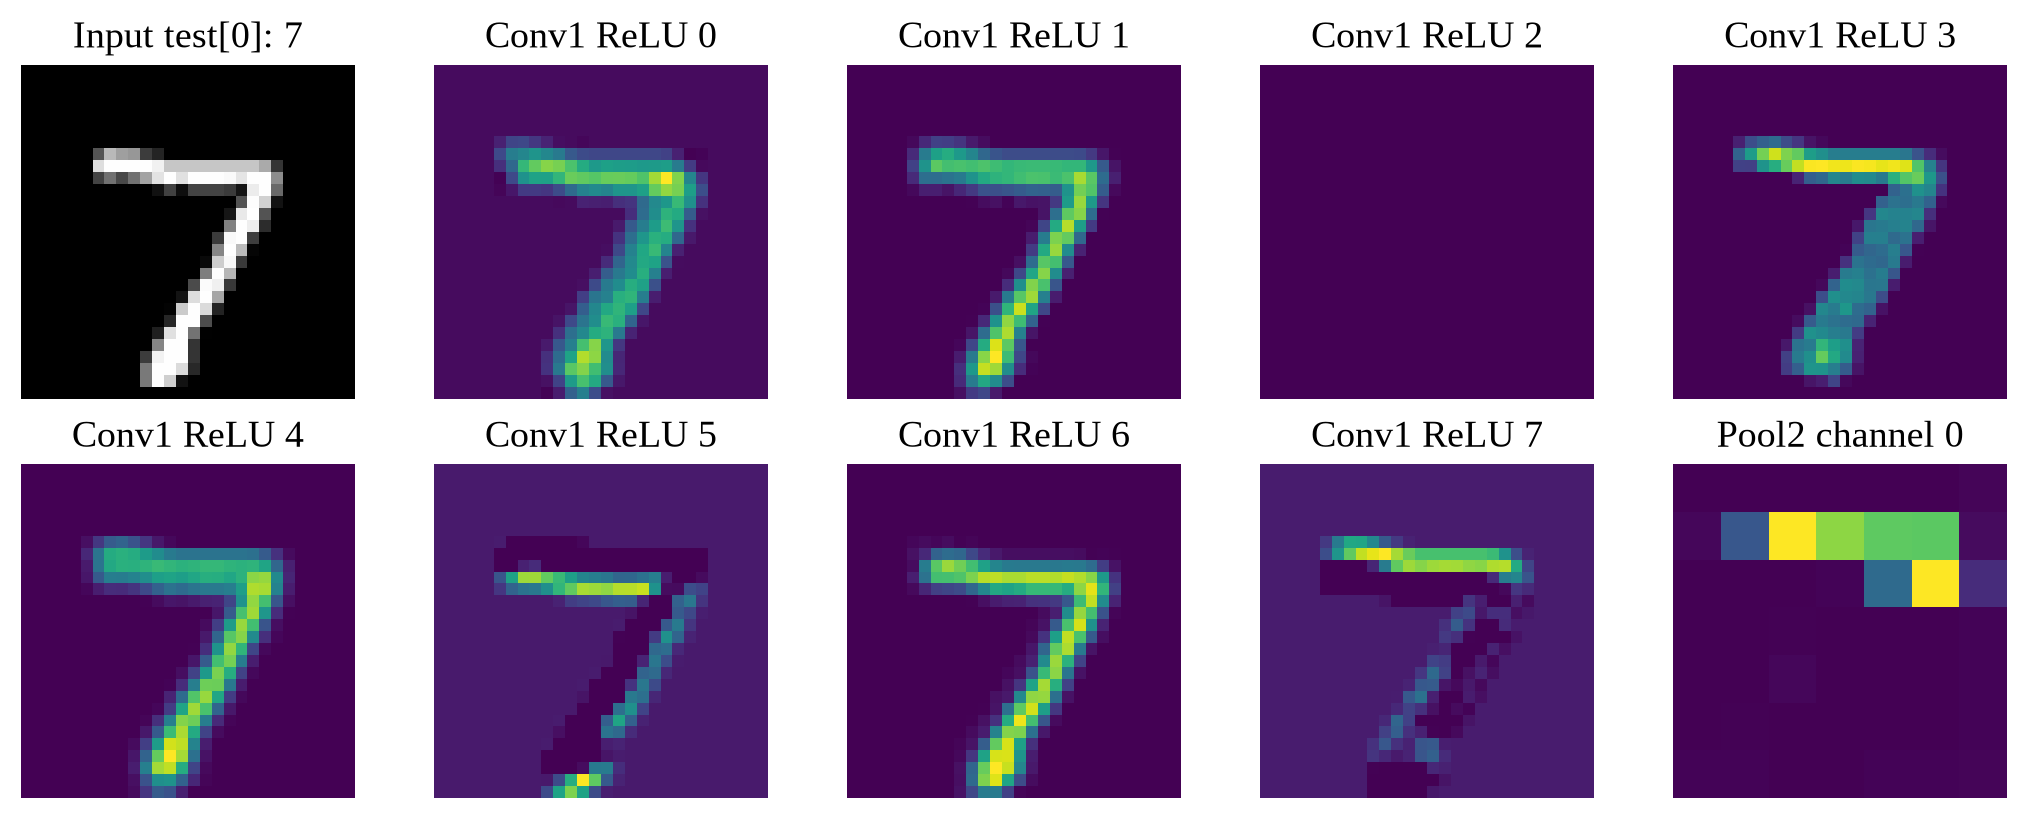
\includegraphics[width=\linewidth,height=.56\textheight,keepaspectratio]{media/media/image11.png}
\caption{Tám feature map sau ReLU tầng 1 và một kênh sau Pool2 của cùng ảnh}\label{fig:legacy-3.3}
\end{figure}



Các feature map cho thấy cùng một ảnh tạo những mức phản ứng khác nhau ở
tám kênh. Mỗi kênh được chuẩn màu riêng khi vẽ nên không nên so độ sáng
tuyệt đối giữa hai ô ảnh như cùng một thang đo. Mục đích là quan sát vị
trí và hình dạng phản ứng; đánh giá độ quan trọng của kênh cần một thí
nghiệm riêng như ablation, chưa được thực hiện ở đây.

Theo chuỗi Conv3--Pool2--Conv3--Pool2 với stride của convolution bằng 1,
vùng tiếp nhận của một phần tử ở đầu ra Pool2 là 10 × 10 pixel và bước
nhảy tương ứng trên ảnh gốc là 4 pixel. Con số này được suy từ kích
thước kernel và stride, không phải kích thước một đối tượng mà mô hình
chắc chắn nhận biết. Sau Flatten, tầng dense kết hợp toàn bộ 16 × 7 × 7
= 784 giá trị nên đầu ra phân loại sử dụng thông tin toàn ảnh.

\Needspace{7\baselineskip}
\captionof{table}{Phân rã 52.138 tham số của mạng}\label{tab:legacy-3.4}

{\def\LTcaptype{none} % do not increment counter
\begin{longtable}[]{@{}
  >{\raggedright\arraybackslash}p{(\linewidth - 4\tabcolsep) * \real{0.2500}}
  >{\centering\arraybackslash}p{(\linewidth - 4\tabcolsep) * \real{0.4999}}
  >{\centering\arraybackslash}p{(\linewidth - 4\tabcolsep) * \real{0.2500}}@{}}
\toprule\noalign{}
\begin{minipage}[b]{\linewidth}\raggedright
\textbf{Khối}
\end{minipage} & \begin{minipage}[b]{\linewidth}\centering
\textbf{Cách tính}
\end{minipage} & \begin{minipage}[b]{\linewidth}\centering
\textbf{Tham số}
\end{minipage} \\
\midrule\noalign{}
\endhead
\bottomrule\noalign{}
\endlastfoot
Conv1 & 8 × (1 × 3 × 3 + 1) & 80 \\
Conv2 & 16 × (8 × 3 × 3 + 1) & 1168 \\
Dense1 & 784 × 64 + 64 & 50240 \\
Dense2 & 64 × 10 + 10 & 650 \\
\end{longtable}
}

Phần lớn tham số nằm ở Dense1, không phải hai tầng tích chập. Điều này
giải thích vì sao tăng kích thước ảnh hoặc số kênh có thể làm mô hình
nặng lên nhanh nếu vẫn Flatten trực tiếp. Với MNIST, kiến trúc nhỏ giúp
huấn luyện CPU và xuất API nhẹ; không có BatchNorm hay Dropout trong
checkpoint dù hai tầng này đã được giới thiệu như các lựa chọn CNN phổ
biến ở phần lý thuyết.

\section{Kết quả và phân tích dự đoán}\label{kux1ebft-quux1ea3-vuxe0-phuxe2n-tuxedch-dux1ef1-ux111ouxe1n}

\Needspace{7\baselineskip}
\captionof{table}{Đánh giá CNN trên các tập độc lập}\label{tab:legacy-3.5}

{\def\LTcaptype{none} % do not increment counter
\begin{longtable}[]{@{}
  >{\raggedright\arraybackslash}p{(\linewidth - 4\tabcolsep) * \real{0.3750}}
  >{\centering\arraybackslash}p{(\linewidth - 4\tabcolsep) * \real{0.3125}}
  >{\centering\arraybackslash}p{(\linewidth - 4\tabcolsep) * \real{0.3125}}@{}}
\toprule\noalign{}
\begin{minipage}[b]{\linewidth}\raggedright
\textbf{Tập}
\end{minipage} & \begin{minipage}[b]{\linewidth}\centering
\textbf{Accuracy}
\end{minipage} & \begin{minipage}[b]{\linewidth}\centering
\textbf{Macro-F1}
\end{minipage} \\
\midrule\noalign{}
\endhead
\bottomrule\noalign{}
\endlastfoot
Validation & 0.9849 & 0.9848 \\
Test 10.000 ảnh & 0.9866 & 0.9865 \\
\end{longtable}
}

\begin{figure}[H]
\centering
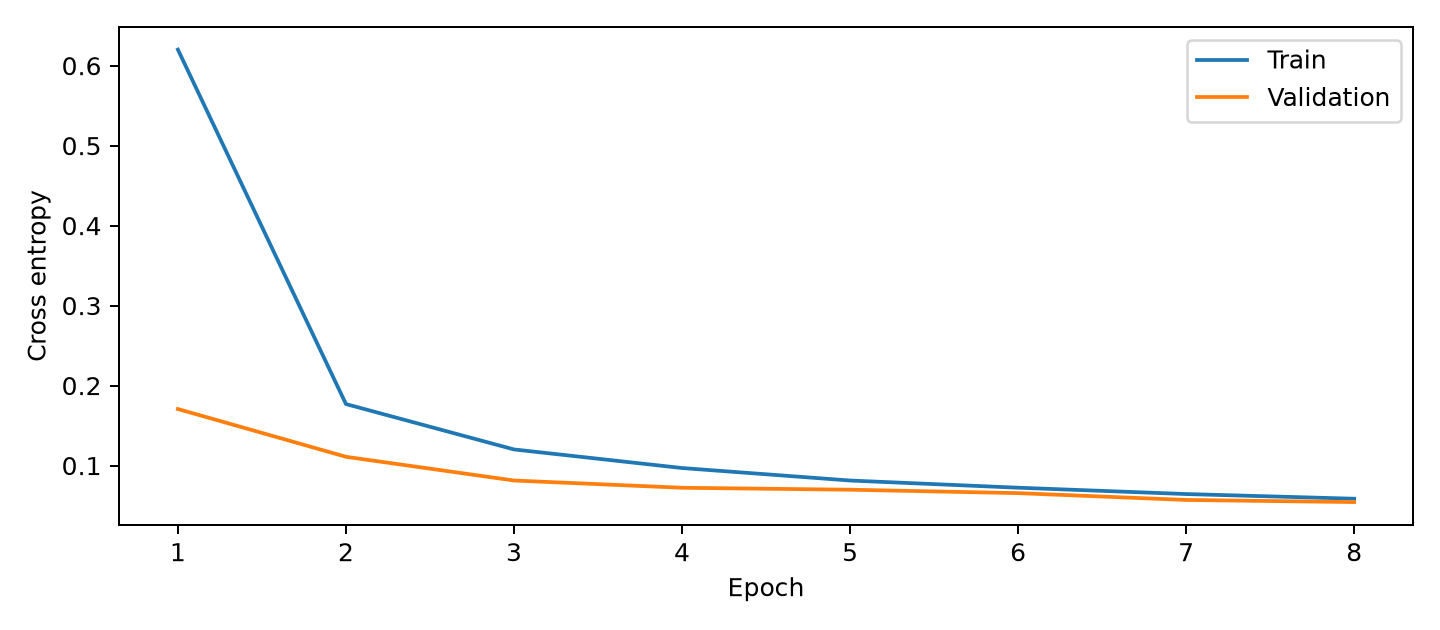
\includegraphics[width=\linewidth,height=.56\textheight,keepaspectratio]{media/media/image12.png}
\caption{Learning curve của CNN qua 8 epoch}\label{fig:legacy-3.4}
\end{figure}

\begin{figure}[H]
\centering
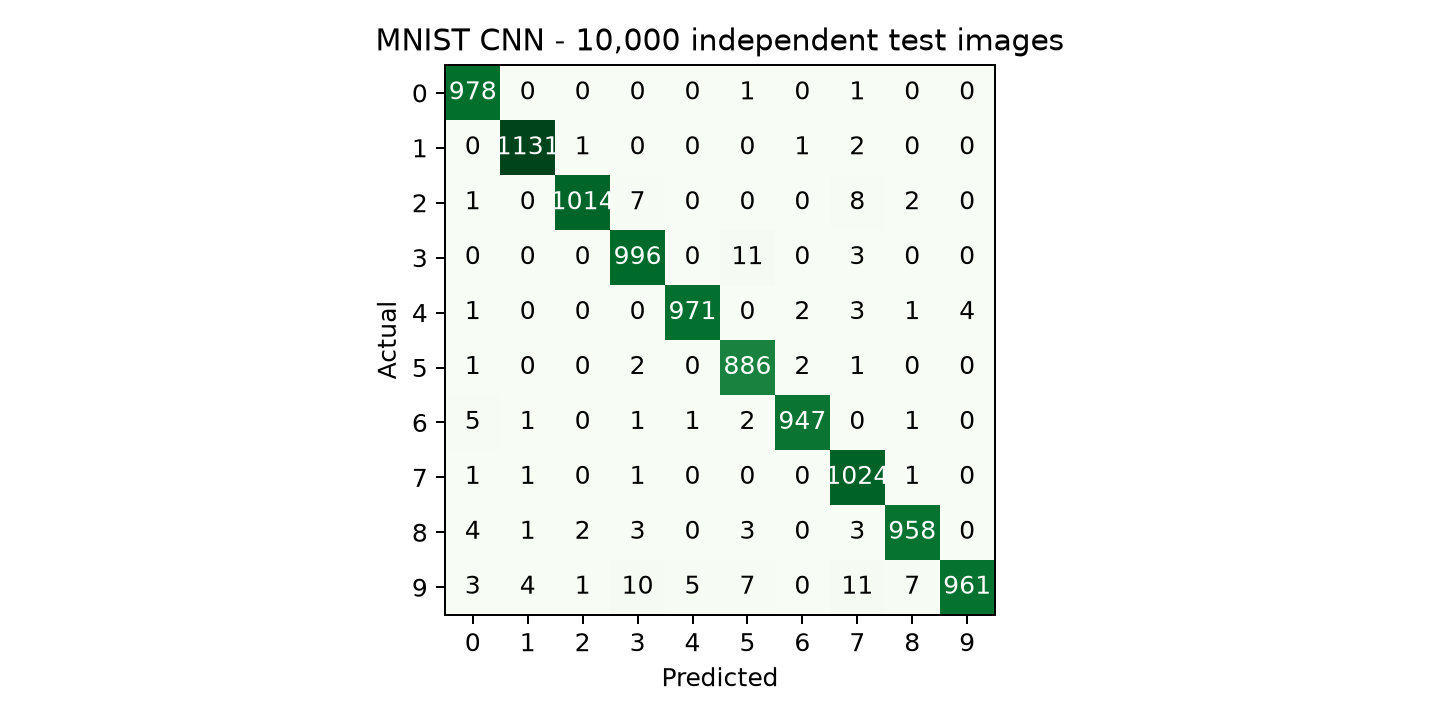
\includegraphics[width=\linewidth,height=.56\textheight,keepaspectratio]{media/media/image13.png}
\caption{Ma trận nhầm lẫn CNN trên tập test MNIST}\label{fig:legacy-3.5}
\end{figure}



\begin{figure}[H]
\centering
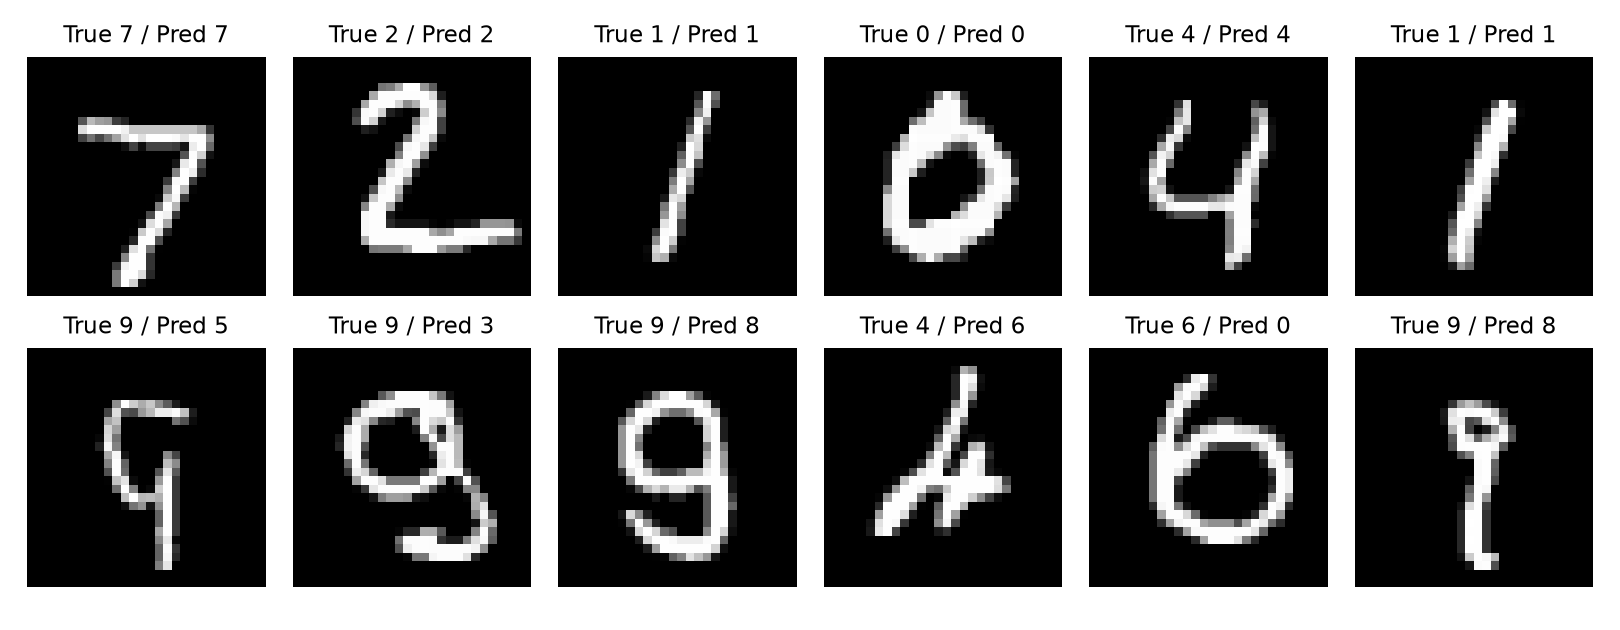
\includegraphics[width=\linewidth,height=.56\textheight,keepaspectratio]{media/media/image14.png}
\caption{Sáu dự đoán đầu và sáu lỗi đầu tiên theo thứ tự test}\label{fig:legacy-3.6}
\end{figure}





Accuracy test là 98.66\%, tương đương 134 lỗi trên 10.000 ảnh. Các ảnh
sai trong Hình 3.6 được chọn bằng quy tắc cố định, không chọn riêng ví
dụ đẹp. Learning curve cho thấy validation loss giảm trong cấu hình đã
chạy; không kết luận mọi CNN hoặc mọi dữ liệu ảnh đều đạt mức này. Ảnh
vẽ tay trên web có thể khác phân phối MNIST nên hiển thị confidence của
mô hình thay cho cam kết đúng.

\subsection{Đọc đường học và đánh giá theo từng chữ số}\label{ux111ux1ecdc-ux111ux1b0ux1eddng-hux1ecdc-vuxe0-ux111uxe1nh-giuxe1-theo-tux1eebng-chux1eef-sux1ed1}

Loss train được đo trong chế độ train có dịch ảnh ngẫu nhiên, còn
validation dùng ảnh nguyên và không cập nhật trọng số. Vì điều kiện đầu
vào khác nhau, loss train không bắt buộc phải thấp hơn validation ở mọi
epoch. Checkpoint epoch 8 được chọn bằng validation loss trong số tám
epoch đã định; không phải bằng kết quả tốt nhất trên test và cũng chưa
chứng minh rằng huấn luyện lâu hơn sẽ luôn tốt hơn.

\Needspace{7\baselineskip}
\captionof{table}{Chỉ số từng chữ số tính từ toàn bộ 10.000 dự đoán test}\label{tab:legacy-3.6}

{\def\LTcaptype{none} % do not increment counter
\begin{longtable}[]{@{}
  >{\raggedright\arraybackslash}p{(\linewidth - 8\tabcolsep) * \real{0.2000}}
  >{\centering\arraybackslash}p{(\linewidth - 8\tabcolsep) * \real{0.2000}}
  >{\centering\arraybackslash}p{(\linewidth - 8\tabcolsep) * \real{0.2000}}
  >{\centering\arraybackslash}p{(\linewidth - 8\tabcolsep) * \real{0.2000}}
  >{\centering\arraybackslash}p{(\linewidth - 8\tabcolsep) * \real{0.2000}}@{}}
\toprule\noalign{}
\begin{minipage}[b]{\linewidth}\raggedright
\textbf{Chữ số}
\end{minipage} & \begin{minipage}[b]{\linewidth}\centering
\textbf{Precision}
\end{minipage} & \begin{minipage}[b]{\linewidth}\centering
\textbf{Recall}
\end{minipage} & \begin{minipage}[b]{\linewidth}\centering
\textbf{F1}
\end{minipage} & \begin{minipage}[b]{\linewidth}\centering
\textbf{Mẫu test}
\end{minipage} \\
\midrule\noalign{}
\endhead
\bottomrule\noalign{}
\endlastfoot
0 & 0.9839 & 0.9980 & 0.9909 & 980 \\
1 & 0.9938 & 0.9965 & 0.9952 & 1135 \\
2 & 0.9961 & 0.9826 & 0.9893 & 1032 \\
3 & 0.9765 & 0.9861 & 0.9813 & 1010 \\
4 & 0.9939 & 0.9888 & 0.9913 & 982 \\
5 & 0.9736 & 0.9933 & 0.9834 & 892 \\
6 & 0.9947 & 0.9885 & 0.9916 & 958 \\
7 & 0.9697 & 0.9961 & 0.9827 & 1028 \\
8 & 0.9876 & 0.9836 & 0.9856 & 974 \\
9 & 0.9959 & 0.9524 & 0.9737 & 1009 \\
\end{longtable}
}

Chữ số 9 có recall khoảng 0,9524, thấp hơn các lớp còn lại trong lần
chạy này. Chữ số 7 có recall cao nhưng precision khoảng 0,9697, nghĩa là
một phần ảnh thuộc lớp khác bị nhận thành 7. Ma trận nhầm lẫn và các ảnh
sai giúp đặt giả thuyết về nét chữ gần nhau; chưa có nhãn nguyên nhân
lỗi, vì vậy không quy toàn bộ lỗi cho một đặc điểm nét viết cụ thể.

\subsection{Confidence không thay thế kiểm tra độ đúng}\label{confidence-khuxf4ng-thay-thux1ebf-kiux1ec3m-tra-ux111ux1ed9-ux111uxfang}

\begin{figure}[H]
\centering
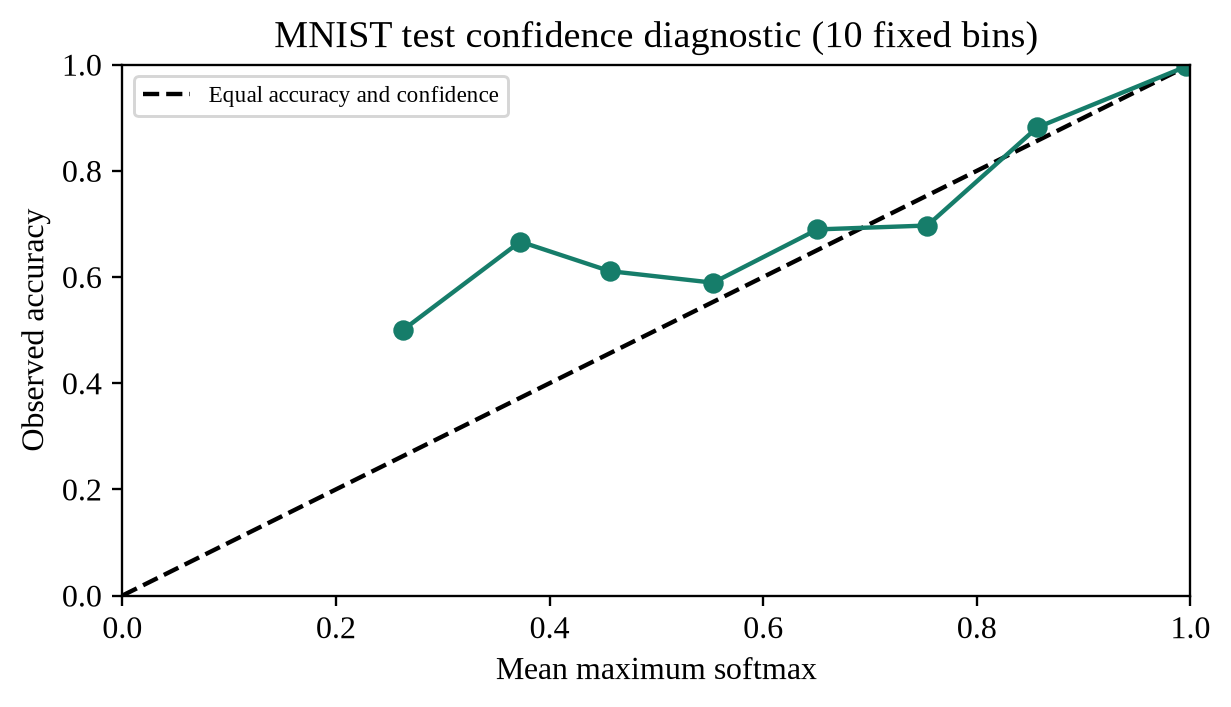
\includegraphics[width=\linewidth,height=.56\textheight,keepaspectratio]{media/media/image15.png}
\caption{Độ đúng quan sát và confidence trung bình trên các khoảng cố định}\label{fig:legacy-3.7}
\end{figure}



Confidence ở đây là softmax lớn nhất. Chia test thành 10 khoảng rộng 0,1
cho ECE mô tả khoảng 0.00243; ECE nhỏ trên tập này không bảo đảm mô hình
nhận được ảnh ngoài phân phối. Có 5 ảnh nhận sai dù confidence ít nhất
99\%. Các khoảng confidence thấp có ít mẫu nên đường biểu diễn dao động
mạnh và không nên diễn giải như một ước lượng ổn định.

Không dùng biểu đồ test này để chọn một ngưỡng từ chối rồi báo lại chính
test như đánh giá độc lập. Nếu muốn bổ sung cơ chế abstention, cần chọn
ngưỡng trên validation hoặc một tập hiệu chỉnh riêng, sau đó kiểm tra cả
tỷ lệ bao phủ và sai số trên phần được chấp nhận. Đây là hướng phát
triển, chưa phải chức năng có hiệu năng được xác minh trong bản hiện
tại.

\subsection{Đường đi của ảnh trên giao diện}\label{ux111ux1b0ux1eddng-ux111i-cux1ee7a-ux1ea3nh-truxean-giao-diux1ec7n}

Ảnh test mẫu được đưa trực tiếp vào API ở dạng 784 pixel; ảnh canvas
được thu từ 280 × 280 xuống 28 × 28 rồi chia 255 giống miền giá trị
train. Bản hiện tại chưa tự căn giữa theo trọng tâm hoặc hiệu chỉnh độ
dày nét. Vì vậy hướng dẫn yêu cầu một chữ số sáng ở giữa nền đen. Việc
công bố đúng bước xử lý có ý nghĩa hơn việc gán Accuracy MNIST cho mọi
ảnh người dùng có thể vẽ.

API đã bổ sung kiểm tra ảnh toàn 0 ở phía máy chủ, ngoài kiểm tra tại
giao diện. Nhờ đó gửi yêu cầu trực tiếp không còn nhận một nhãn tưởng
như hợp lệ cho ảnh trống. Các lỗi thiếu pixel, pixel ngoài 0--255 hoặc
NaN cũng bị từ chối. Thay đổi này cải thiện tính đúng đắn của dịch vụ;
không được tính là tăng Accuracy của checkpoint vì trọng số không thay
đổi.

\productlink{Truy cập sản phẩm thực nghiệm}{https://rag-httm-chatbot.vercel.app/?demo=cnn\#experiments}

\begin{figure}[H]
\centering
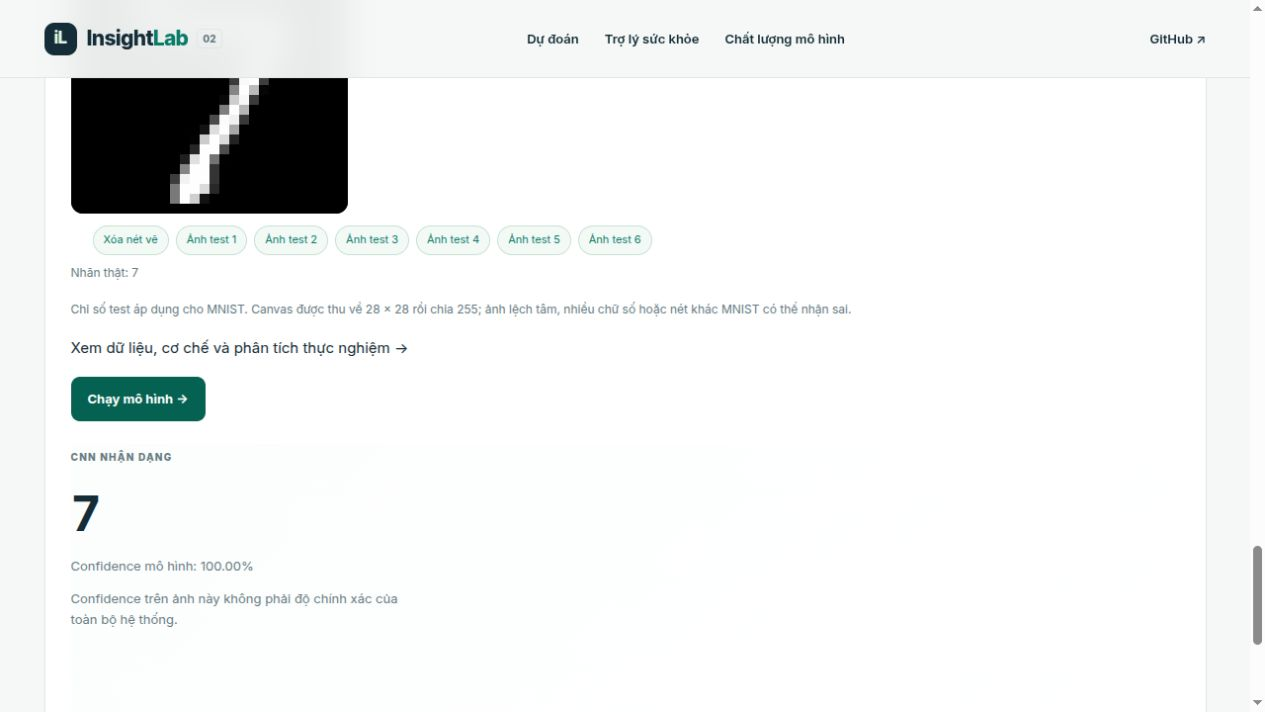
\includegraphics[width=\linewidth,height=.56\textheight,keepaspectratio]{media/media/image16.png}
\caption{Giao diện thực nghiệm: ảnh test nhãn 7 được API nhận dạng thành 7}\label{fig:legacy-3.8}
\end{figure}



\section{Suy luận, triển khai và phạm vi mở rộng}\label{suy-luux1eadn-triux1ec3n-khai-vuxe0-phux1ea1m-vi-mux1edf-rux1ed9ng}

Checkpoint PyTorch được xuất thành trọng số JSON. API thực hiện
convolution, ReLU, max-pooling, flatten và dense bằng đúng trọng số đã
huấn luyện, dùng Python standard library để tránh đóng gói PyTorch nặng
vào serverless. Bộ vector đối chiếu kiểm tra logits của API với PyTorch.
Giao diện hỗ trợ ảnh test thật, canvas vẽ số, kiểm tra ảnh trống, trạng
thái đang xử lý và thông báo lỗi.

ASL được giữ như ví dụ mở rộng của bài toán thị giác: các cử chỉ M/N
hoặc U/V gần nhau, nền ảnh và góc chụp có thể làm giảm khả năng tổng
quát hóa. Trong lần thực hiện này chưa huấn luyện lại ASL, vì vậy các
accuracy và biểu đồ ASL cũ không được dùng như kết quả mới. Tương tự,
không khẳng định Keras và PyTorch tương đương từ một phép thử chỉ chạy
PyTorch.

\chapter{Mạng nơ-ron hồi tiếp RNN}\label{chux1b0ux1a1ng-4.-mux1ea1ng-nux1a1-ron-hux1ed3i-tiux1ebfp-RNN}

Đối với chuỗi giá, thứ tự quan sát quyết định thông tin nào thực sự có
sẵn tại thời điểm dự báo. Chia ngẫu nhiên các cửa sổ chồng lấn có thể
làm mô hình nhìn gián tiếp vào tương lai. Hơn nữa, giá ngày mai thường
gần giá hôm nay, nên một đường dự báo bám sát giá thực chưa chứng minh
mạng đã học được tín hiệu hữu ích.

Chương xây bài toán dự báo một bước bằng 30 log-return đã biết và so
sánh RNN, LSTM, GRU với Persistence. Phép chia theo ngày của nhãn, chuẩn
hóa chỉ trên train và lựa chọn bằng validation được đặt trước việc đánh
giá test. Hai chuỗi FPT và vàng futures cho phép kiểm tra liệu kết luận
có nhất quán giữa các miền hay không.

Nội dung chính gồm cơ chế nhớ và cổng, cách tạo cửa sổ, quy trình huấn
luyện, đường học và sai số theo đơn vị giá. Phân tích độ bất định bổ
sung cho so sánh điểm MAE; phần triển khai giải thích vì sao một
baseline đơn giản vẫn có thể được chọn cho web.

\section{Lý thuyết RNN}\label{luxfd-thuyux1ebft-RNN}

\subsection{Vấn đề với dữ liệu tuần tự}\label{vux1ea5n-ux111ux1ec1-vux1edbi-dux1eef-liux1ec7u-tuux1ea7n-tux1ef1}

Dense layer không giữ trạng thái qua thời gian. CNN có thể xử lý tín
hiệu 1D theo trường tiếp nhận hữu hạn; RNN bổ sung trạng thái truyền qua
các bước để biểu diễn ngữ cảnh của chuỗi.

\begin{quote}
• Giá hôm nay phụ thuộc vào giá hôm qua

• Từ trong câu phụ thuộc vào từ trước đó

• Nhịp tim tương lai phụ thuộc vào lịch sử

→ Cần kiến trúc có bộ nhớ (memory) giữa các bước thời gian.
\end{quote}

\subsection{RNN cơ bản --- Vanilla RNN}\label{RNN-cux1a1-bux1ea3n-vanilla-RNN}

Tại mỗi bước thời gian t:

\(\begin{array}{r}
h_{t} = \tanh(W_{x}x_{t} + W_{h}h_{t - 1} + b) \\
{\hat{y}}_{t} = W_{y}h_{t} + b_{y}
\end{array}\) (4.1)

Trong đó:

\begin{quote}
• xi: vector đầu vào tại bước t

• hi: hidden state (bộ nhớ ngắn hạn)

• Wx, Wh và Wγ là ma trận trọng số; các tham số được dùng chung tại mọi
bước thời gian.
\end{quote}

Backpropagation Through Time (BPTT):

\(\frac{\partial\mathcal{L}}{\partial\theta} = \sum_{t = 1}^{T}{\sum_{k = 1}^{t}\frac{\partial\mathcal{L}_{t}}{\partial h_{t}}}\frac{\partial h_{t}}{\partial h_{k}}\left( \frac{\partial h_{k}}{\partial\theta} \right)_{direct}\)
(4.2)

θ là một tham số dùng chung của mạng; đạo hàm cuối chỉ lấy tác động trực
tiếp tại bước k. Tổng theo k cộng các đường mà tham số ảnh hưởng tới
loss ở bước t. Đạo hàm giữa hai trạng thái bao gồm toàn bộ các bước
trung gian, với đạo hàm đồng nhất khi k=t.

\subsection{LSTM --- Long Short-Term Memory}\label{LSTM-long-short-term-memory}

LSTM thêm cell state ct như "bộ nhớ dài hạn" và 3 gates kiểm soát luồng
thông tin:

Forget Gate: Quyết định quên bao nhiêu cell state cũ

\(f_{t} = \sigma(W_{f}\lbrack h_{t - 1},x_{t}\rbrack + b_{f})\) (4.3)

Input Gate: Quyết định thêm thông tin mới nào

\(i_{t} = \sigma(W_{i}\lbrack h_{t - 1},x_{t}\rbrack + b_{i}),\quad{\tilde{c}}_{t} = \tanh(W_{c}\lbrack h_{t - 1},x_{t}\rbrack + b_{c})\)
(4.4)

Cập nhật Cell State:

\(c_{t} = f_{t} \odot c_{t - 1} + i_{t} \odot {\tilde{c}}_{t}\) (4.5)

Output Gate: Quyết định đầu ra

\(o_{t} = \sigma(W_{o}\lbrack h_{t - 1},x_{t}\rbrack + b_{o}),\quad h_{t} = o_{t} \odot \tanh(c_{t})\)
(4.6)

\subsection{GRU --- Gated Recurrent Unit}\label{GRU-gated-recurrent-unit}

GRU đơn giản hóa LSTM bằng cách gộp forget gate và input gate thành
update gate:

\(\begin{array}{r}
z_{t} = \sigma(W_{z}\lbrack h_{t - 1},x_{t}\rbrack + b_{z}) \\
r_{t} = \sigma(W_{r}\lbrack h_{t - 1},x_{t}\rbrack + b_{r}) \\
{\tilde{h}}_{t} = \tanh(W\lbrack r_{t} \odot h_{t - 1},x_{t}\rbrack + b) \\
h_{t} = (1 - z_{t}) \odot h_{t - 1} + z_{t} \odot {\tilde{h}}_{t}
\end{array}\) (4.7)

\Needspace{7\baselineskip}
\captionof{table}{So sánh cấu trúc recurrent network}\label{tab:legacy-4.1}

{\def\LTcaptype{none} % do not increment counter
\begin{longtable}[]{@{}
  >{\raggedright\arraybackslash}p{(\linewidth - 6\tabcolsep) * \real{0.1250}}
  >{\centering\arraybackslash}p{(\linewidth - 6\tabcolsep) * \real{0.2500}}
  >{\centering\arraybackslash}p{(\linewidth - 6\tabcolsep) * \real{0.2500}}
  >{\raggedright\arraybackslash}p{(\linewidth - 6\tabcolsep) * \real{0.3750}}@{}}
\toprule\noalign{}
\begin{minipage}[b]{\linewidth}\raggedright
\textbf{Mạng}
\end{minipage} & \begin{minipage}[b]{\linewidth}\centering
\textbf{Trạng thái}
\end{minipage} & \begin{minipage}[b]{\linewidth}\centering
\textbf{Số cổng}
\end{minipage} & \begin{minipage}[b]{\linewidth}\centering
\textbf{Đặc điểm}
\end{minipage} \\
\midrule\noalign{}
\endhead
\bottomrule\noalign{}
\endlastfoot
RNN & Hidden state ht & Không có cổng & Ít tham số, khó học phụ thuộc
xa \\
LSTM & ht và cell state ct & Input, forget, output & Luồng cộng qua cell
state hỗ trợ truyền gradient \\
GRU & Hidden state ht & Reset và update & Ít tham số hơn LSTM cùng kích
thước ẩn \\
\end{longtable}
}

\subsection{Cửa sổ trượt và các kiểu đầu vào đầu ra}\label{cux1eeda-sux1ed5-trux1b0ux1ee3t-vuxe0-cuxe1c-kiux1ec3u-ux111ux1ea7u-vuxe0o-ux111ux1ea7u-ra}

Cửa sổ trượt tạo một mẫu bằng L quan sát quá khứ và nhãn của bước kế
tiếp. Many-to-one ánh xạ chuỗi thành một giá trị hoặc nhãn; one-to-many
sinh chuỗi từ một ngữ cảnh đầu; many-to-many tạo một đầu ra ở mỗi bước
hoặc một chuỗi đầu ra khác độ dài. Thực nghiệm dự báo giá trong chương
sử dụng many-to-one.

\(X_{t} = \lbrack r_{t - L + 1},\ldots,r_{t}\rbrack,\quad r_{t} = \log(P_{t}/P_{t - 1}),\quad{\hat{P}}_{t + 1} = P_{t}e^{{\hat{r}}_{t + 1}}\)
(4.8)

Pt là giá đóng cửa, rt là log-return, L=30 là chiều dài cửa sổ. Dự báo
tại t dùng dữ liệu không muộn hơn t; nhãn ở t+1. Mỗi cửa sổ khởi tạo
trạng thái ẩn bằng 0 và không truyền hidden state từ test về train.

\subsection{BPTT và ổn định gradient}\label{bptt-vuxe0-ux1ed5n-ux111ux1ecbnh-gradient}

\(\frac{\partial h_{t}}{\partial h_{t - k}} = \prod_{j = t - k + 1}^{t}\frac{\partial h_{j}}{\partial h_{j - 1}}\)
(4.9)

BPTT trải mạng theo thời gian và cộng gradient của cùng tham số qua các
bước. Tích nhiều Jacobian có chuẩn nhỏ hơn 1 có thể làm gradient suy
giảm, còn chuẩn lớn có thể gây bùng nổ. LSTM/GRU tạo đường truyền có
cổng để giảm khó khăn này nhưng không bảo đảm giải quyết mọi phụ thuộc
dài hạn. Gradient clipping giới hạn norm; chuẩn hóa chỉ trên train và
chọn checkpoint bằng validation giúp ổn định thực nghiệm.

\section{Dữ liệu, phép chia và cấu hình}\label{dux1eef-liux1ec7u-phuxe9p-chia-vuxe0-cux1ea5u-huxecnh}

Dùng bản chụp dữ liệu Yahoo Finance của Tiểu luận 02: FPT.VN có 1.304 phiên và
vàng futures GC=F có 1.257 phiên, từ 15/10/2021 đến 14/10/2026. GC=F
không được đổi tên thành spot XAU/USD. Lợi suất được tính theo phiên có
thật, không nội suy ngày nghỉ. Dữ liệu e-commerce không được đưa vào
thực nghiệm mới vì chưa xác minh được thứ tự sự kiện và nhãn đủ để biện
minh cho RNN.

Ngày của nhãn quyết định tập dữ liệu: FPT train trước 13/02/2026,
validation từ 13/02 đến trước 04/06/2026; vàng train trước 26/02/2026,
validation đến trước 09/06/2026. Test kéo dài đến nhãn 14/10/2026. Cách
định nghĩa này khác chỉ số ngày đặc trưng của bảng thị trường ở Chương
5; không so sánh trực tiếp hai bảng như cùng tập test. Validation/test
được phép dùng lịch sử đã biết trước ngày nhãn, phù hợp dự báo cuốn
chiếu một bước.

\Needspace{7\baselineskip}
\captionof{table}{Phân chia chuỗi theo ngày nhãn}\label{tab:legacy-4.2}

{\def\LTcaptype{none} % do not increment counter
\begin{longtable}[]{@{}
  >{\raggedright\arraybackslash}p{(\linewidth - 4\tabcolsep) * \real{0.1875}}
  >{\centering\arraybackslash}p{(\linewidth - 4\tabcolsep) * \real{0.3125}}
  >{\centering\arraybackslash}p{(\linewidth - 4\tabcolsep) * \real{0.4999}}@{}}
\toprule\noalign{}
\begin{minipage}[b]{\linewidth}\raggedright
\textbf{Miền}
\end{minipage} & \begin{minipage}[b]{\linewidth}\centering
\textbf{Train / Val / Test}
\end{minipage} & \begin{minipage}[b]{\linewidth}\centering
\textbf{Khoảng ngày nhãn test}
\end{minipage} \\
\midrule\noalign{}
\endhead
\bottomrule\noalign{}
\endlastfoot
FPT & 1099 / 79 / 95 & 2026-06-04 --- 2026-10-14 \\
Gold & 1066 / 71 / 89 & 2026-06-09 --- 2026-10-14 \\
\end{longtable}
}

Ba mạng dùng 16 hidden units, một recurrent layer và một linear head,
Adam learning\_rate=0,001, 35 epoch, batch\_size=128 và seed=42. Trung
bình và độ lệch chuẩn của đầu vào/nhãn chỉ tính trên train. Checkpoint
tối thiểu validation MSE được lưu; mạng triển khai được chọn bằng
validation MAE theo đơn vị giá, có Persistence cùng tham gia. Test được
giữ cho báo cáo cuối.

GRU trong PyTorch có hai khác biệt quy ước so với công thức lý thuyết ở
trên: reset gate nhân sau phép biến đổi tuyến tính của hidden state
trong nhánh ứng viên; update gate z đặt trọng số lên trạng thái cũ thay
vì ứng viên. Cụ thể, ht=(1−zt)\ensuremath{\odot}nt+zt\ensuremath{\odot}ht−1, với nt là ứng viên. API dùng
đúng hai quy ước của checkpoint; kiểm thử cả sáu mạng phát hiện sai khác
thứ tự cổng, vị trí reset và cách phối hợp trạng thái.

\subsection{Từ giá quan sát đến một mẫu dự báo cụ thể}\label{tux1eeb-giuxe1-quan-suxe1t-ux111ux1ebfn-mux1ed9t-mux1eabu-dux1ef1-buxe1o-cux1ee5-thux1ec3}

\begin{figure}[H]
\centering
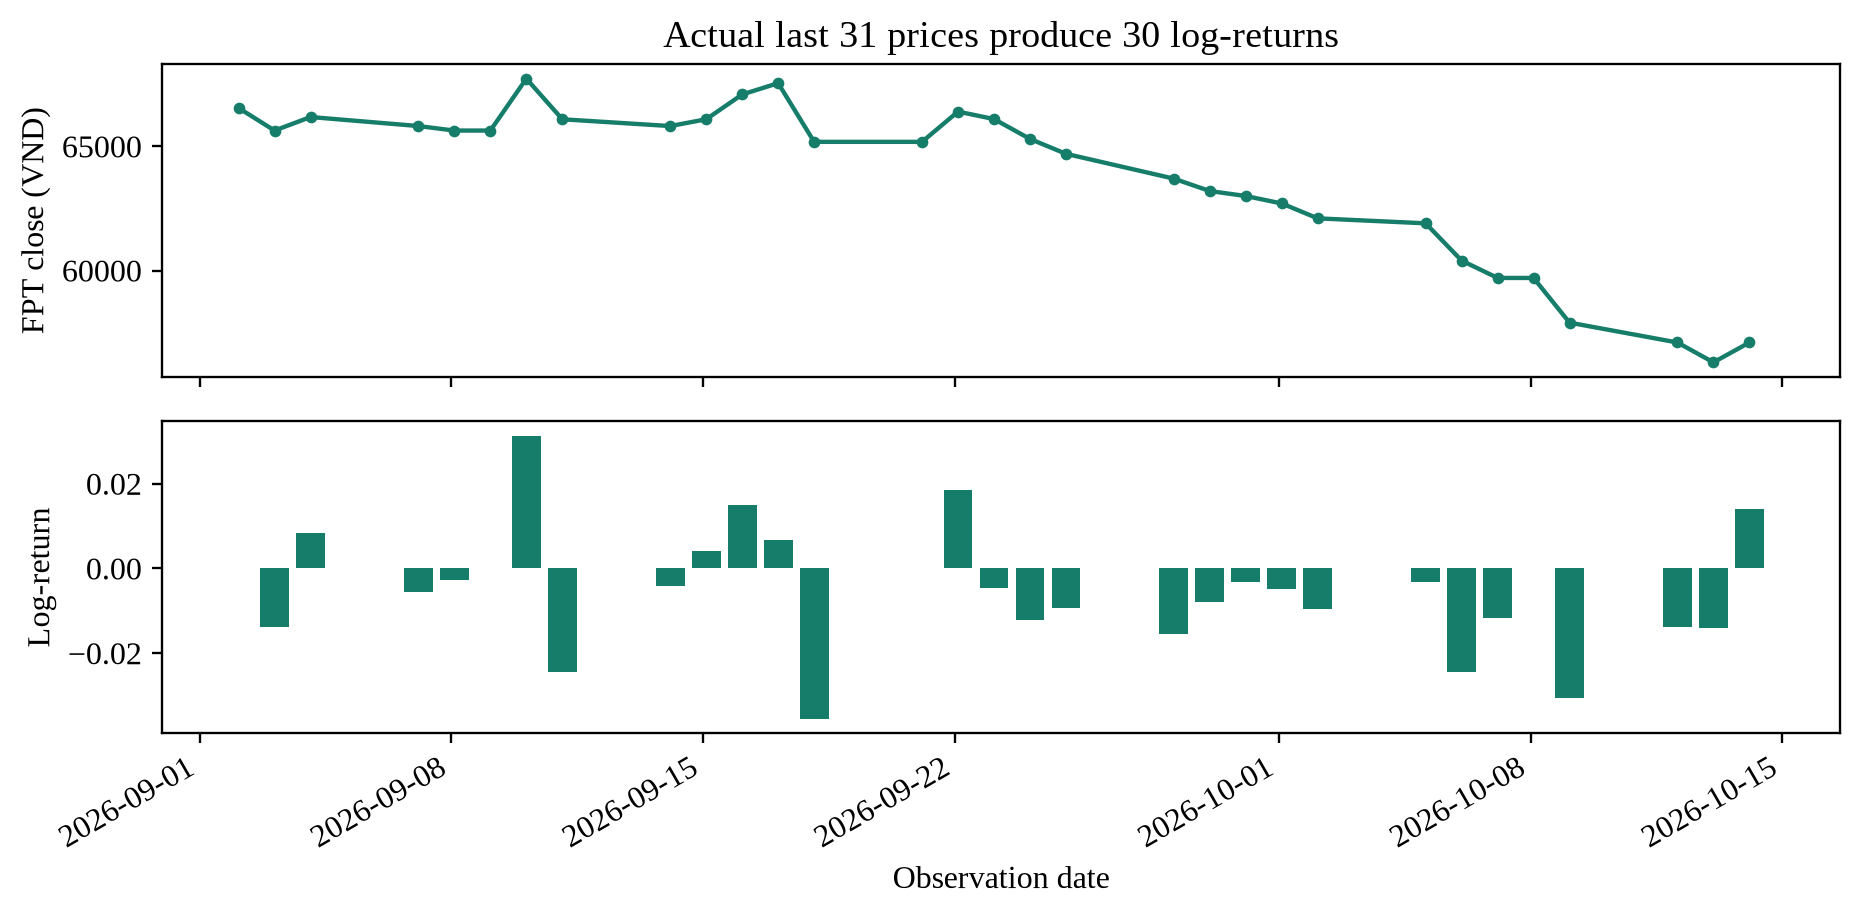
\includegraphics[width=\linewidth,height=.56\textheight,keepaspectratio]{media/media/image17.png}
\caption{31 giá FPT cuối bản chụp dữ liệu và 30 log-return được tính từ chúng}\label{fig:legacy-4.1}
\end{figure}



Cửa sổ minh họa lấy từ 2026-09-02 đến 2026-10-14, gồm 31 giá đóng cửa để
tạo 30 log-return. Hai giá cuối là 56,300 và 57,100 VND, tạo log-return
cuối 0.01410958. Đây chính là một phần đầu vào mặc định của demo, không
phải một chuỗi được đặt số để làm đẹp hình. Snapshot dừng ở 14/10/2026;
dự báo tiếp theo sau cửa sổ không được gọi là giá đã xác minh của ngày
hiện tại.

\begin{figure}[H]
\centering
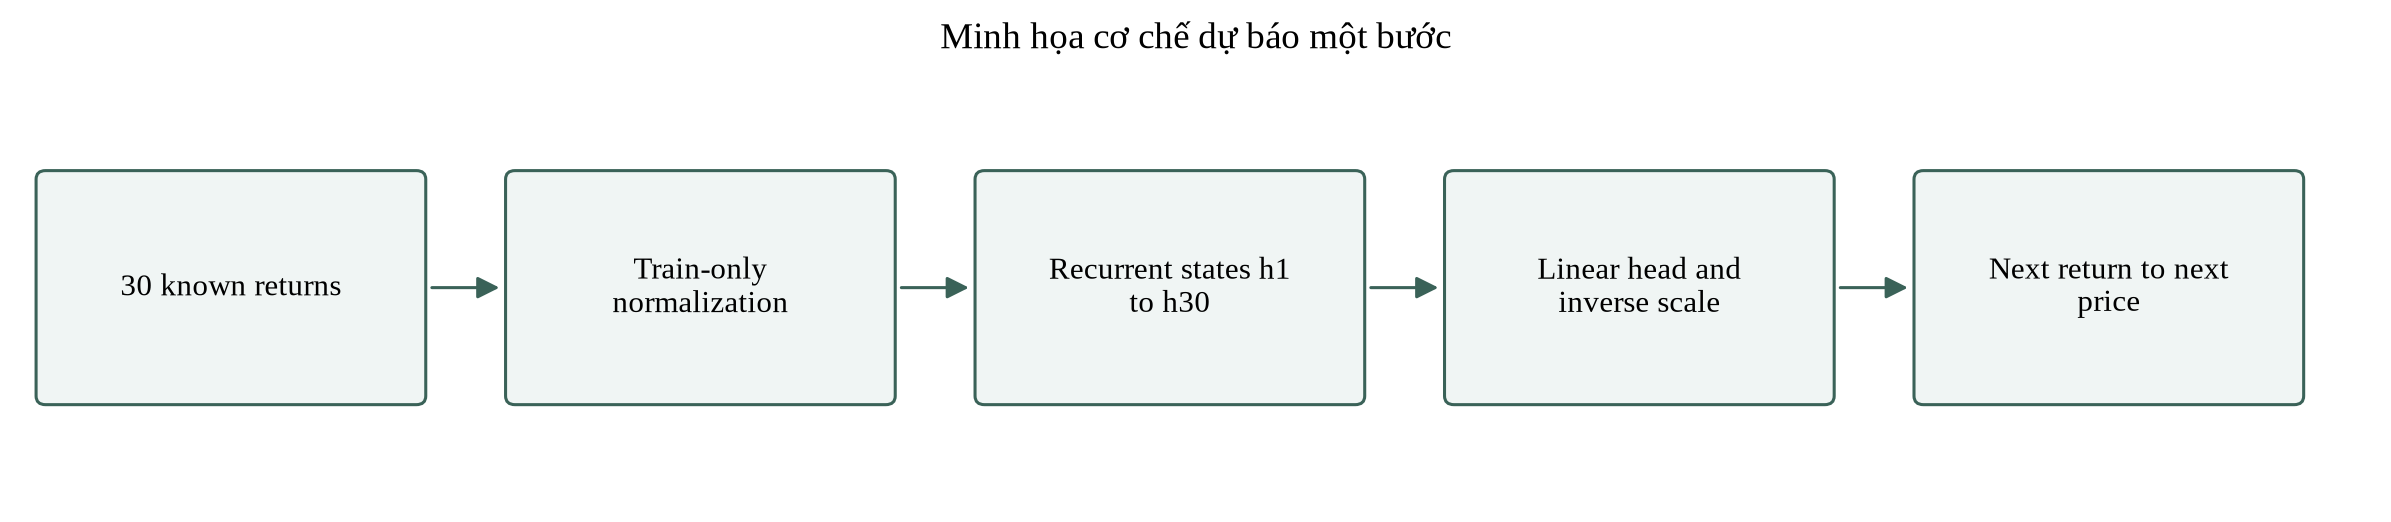
\includegraphics[width=\linewidth,height=.56\textheight,keepaspectratio]{media/media/image18.png}
\caption{Minh họa cơ chế many-to-one và biến đổi ngược về giá}\label{fig:legacy-4.2}
\end{figure}



Mạng nhận tensor {[}batch, 30, 1{]}, không nhận trực tiếp lịch ngày hoặc
mức giá tuyệt đối. Đầu vào là log-return được chuẩn hóa bằng trung bình
và độ lệch chuẩn train. Trạng thái ở bước cuối đi qua Linear(16,1), sau
đó đầu ra được đưa về thang log-return bằng tham số nhãn train. Cuối
cùng nhân giá gần nhất với exp của log-return dự đoán để ra mức giá một
bước tiếp theo.

Chọn log-return giảm sự phụ thuộc trực tiếp vào mức giá và giữ giá dự
đoán dương sau biến đổi ngược. Tuy vậy phân phối lợi suất vẫn có thể
thay đổi theo chế độ thị trường, và mẫu 30 bước không chứa đầy đủ tin
tức hoặc điều kiện vĩ mô. Hai chuỗi dùng checkpoint riêng; không chuyển
trọng số FPT sang vàng hoặc chuẩn hóa chung bằng dữ liệu của cả hai
miền.

\subsection{Vai trò của trạng thái và cổng trong thực nghiệm}\label{vai-truxf2-cux1ee7a-trux1ea1ng-thuxe1i-vuxe0-cux1ed5ng-trong-thux1ef1c-nghiux1ec7m}

Vanilla RNN cập nhật cùng một trạng thái ẩn qua 30 bước; mọi thông tin
cần dùng phải được nén vào vector đó. LSTM có trạng thái ô nhớ và các
cổng để điều tiết lượng thông tin cũ giữ lại, lượng ứng viên được ghi
vào và phần được phát ra. GRU kết hợp cơ chế cập nhật và reset trong một
trạng thái. Những cấu trúc này mở ra đường truyền khác cho thông tin và
gradient, nhưng việc cổng có giúp bài toán cụ thể hay không vẫn phải
kiểm tra bằng thực nghiệm.

Các mạng dùng cùng độ rộng 16, cùng optimizer, số epoch và quy tắc
checkpoint để giảm khác biệt không cần thiết. Số tham số vẫn không bằng
nhau vì LSTM và GRU có nhiều nhánh cổng. Đây là so sánh trong một cấu
hình kiểm soát, chưa phải tìm kiếm tối ưu công bằng theo cùng số phép
tính hoặc cùng số tham số. Không kết luận một họ mạng nói chung kém hơn
chỉ từ cấu hình duy nhất này.

\section{So sánh RNN, LSTM, GRU và Persistence}\label{so-suxe1nh-RNN-LSTM-GRU-vuxe0-persistence}

\Needspace{7\baselineskip}
\captionof{table}{Kết quả mạng chuỗi trong đơn vị gốc VND hoặc USD/oz}\label{tab:legacy-4.3}

{\def\LTcaptype{none} % do not increment counter
\begin{longtable}[]{@{}
  >{\raggedright\arraybackslash}p{(\linewidth - 8\tabcolsep) * \real{0.2500}}
  >{\centering\arraybackslash}p{(\linewidth - 8\tabcolsep) * \real{0.1250}}
  >{\centering\arraybackslash}p{(\linewidth - 8\tabcolsep) * \real{0.2062}}
  >{\centering\arraybackslash}p{(\linewidth - 8\tabcolsep) * \real{0.2062}}
  >{\centering\arraybackslash}p{(\linewidth - 8\tabcolsep) * \real{0.2125}}@{}}
\toprule\noalign{}
\begin{minipage}[b]{\linewidth}\raggedright
\textbf{Miền / Mạng}
\end{minipage} & \begin{minipage}[b]{\linewidth}\centering
\textbf{Tham số}
\end{minipage} & \begin{minipage}[b]{\linewidth}\centering
\textbf{Val MAE}
\end{minipage} & \begin{minipage}[b]{\linewidth}\centering
\textbf{Test MAE}
\end{minipage} & \begin{minipage}[b]{\linewidth}\centering
\textbf{Test RMSE}
\end{minipage} \\
\midrule\noalign{}
\endhead
\bottomrule\noalign{}
\endlastfoot
FPT / RNN & 321 & 1270.880 & 720.604 & 1032.599 \\
FPT / LSTM & 1233 & 1271.182 & 745.759 & 1050.320 \\
FPT / GRU & 929 & 1265.027 & 737.054 & 1044.655 \\
Gold / RNN & 321 & 63.676 & 47.342 & 61.988 \\
Gold / LSTM & 1233 & 63.707 & 48.168 & 63.044 \\
Gold / GRU & 929 & 63.622 & 48.097 & 62.834 \\
\end{longtable}
}

FPT: Persistence test MAE 734.258 VND. Mạng có validation MAE thấp nhất
là GRU (1265.027), trong khi Persistence validation MAE 1266.974. Vì vậy
quy tắc trước test chọn GRU để trình diễn trên web.

GOLD: Persistence test MAE 48.089 USD/oz. Mạng có validation MAE thấp
nhất là GRU (63.622), trong khi Persistence validation MAE 63.152. Vì
vậy quy tắc trước test chọn Persistence để trình diễn trên web.

\begin{figure}[H]
\centering
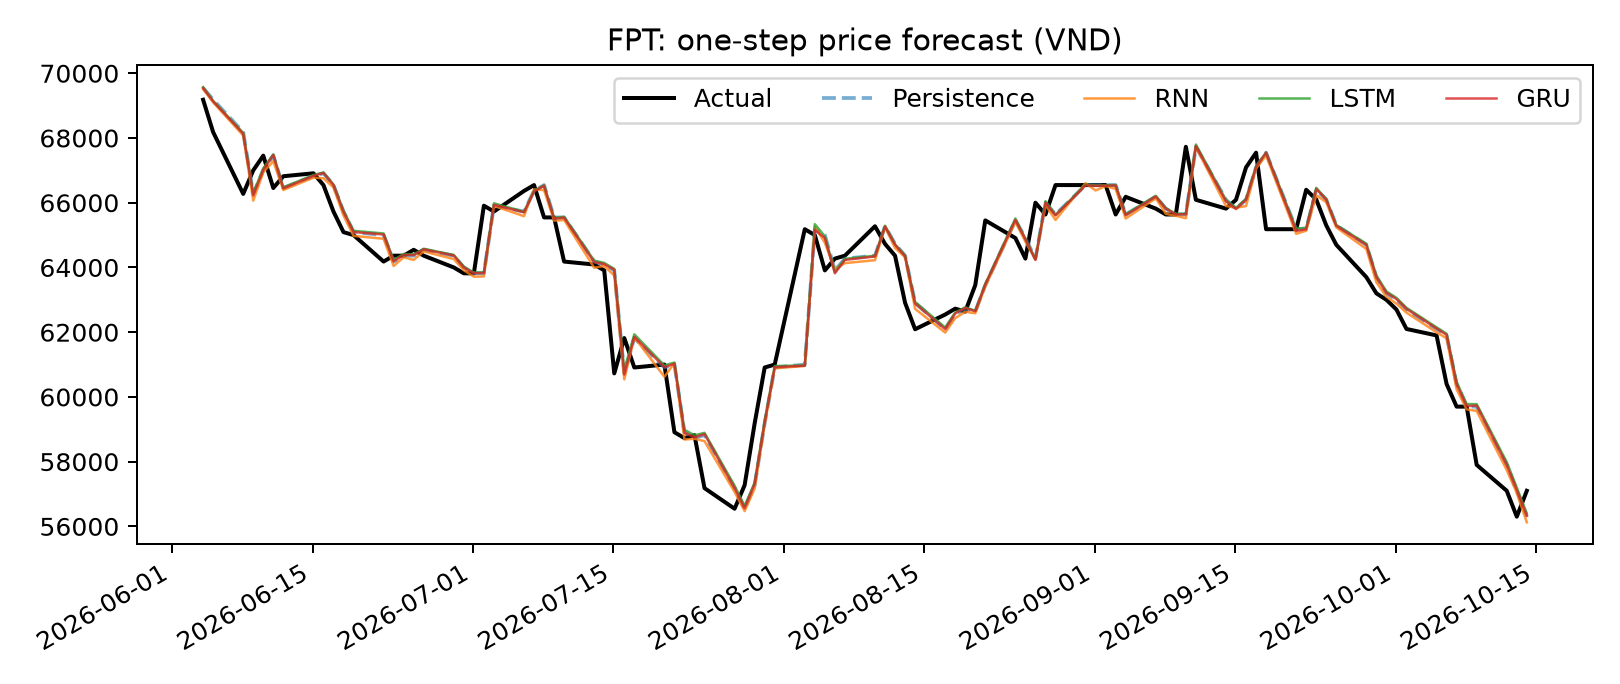
\includegraphics[width=\linewidth,height=.56\textheight,keepaspectratio]{media/media/image19.png}
\caption{Dự báo một bước FPT bằng ba mạng và baseline}\label{fig:legacy-4.3}
\end{figure}

\begin{figure}[H]
\centering
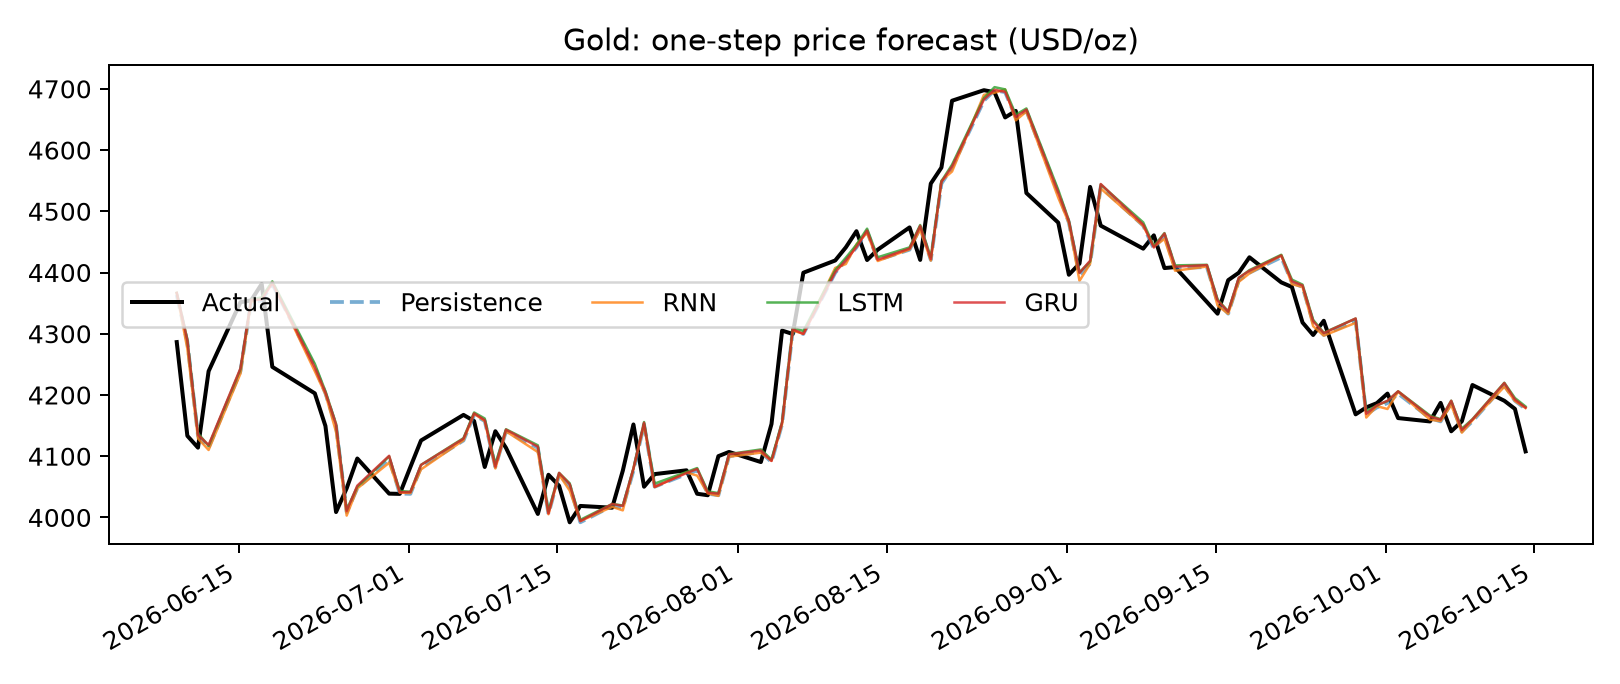
\includegraphics[width=\linewidth,height=.56\textheight,keepaspectratio]{media/media/image20.png}
\caption{Dự báo một bước vàng futures GC=F}\label{fig:legacy-4.4}
\end{figure}





Vanilla RNN có MAE test thấp nhất trong ba mạng ở cả hai miền trong lần
chạy này, nhưng không được đổi lựa chọn triển khai sau khi nhìn test.
Kết quả bác bỏ việc mặc định LSTM luôn tốt hơn. Chuỗi ngắn, ít dữ liệu,
nhiễu thị trường và một random seed hạn chế khả năng khái quát hóa. Mức
chênh MAE nhỏ chưa chứng minh lợi ích giao dịch; báo cáo không suy ra
lợi nhuận.

\subsection{Đường học và tính nhất quán của quy tắc lựa chọn}\label{ux111ux1b0ux1eddng-hux1ecdc-vuxe0-tuxednh-nhux1ea5t-quuxe1n-cux1ee7a-quy-tux1eafc-lux1ef1a-chux1ecdn}

\begin{figure}[H]
\centering
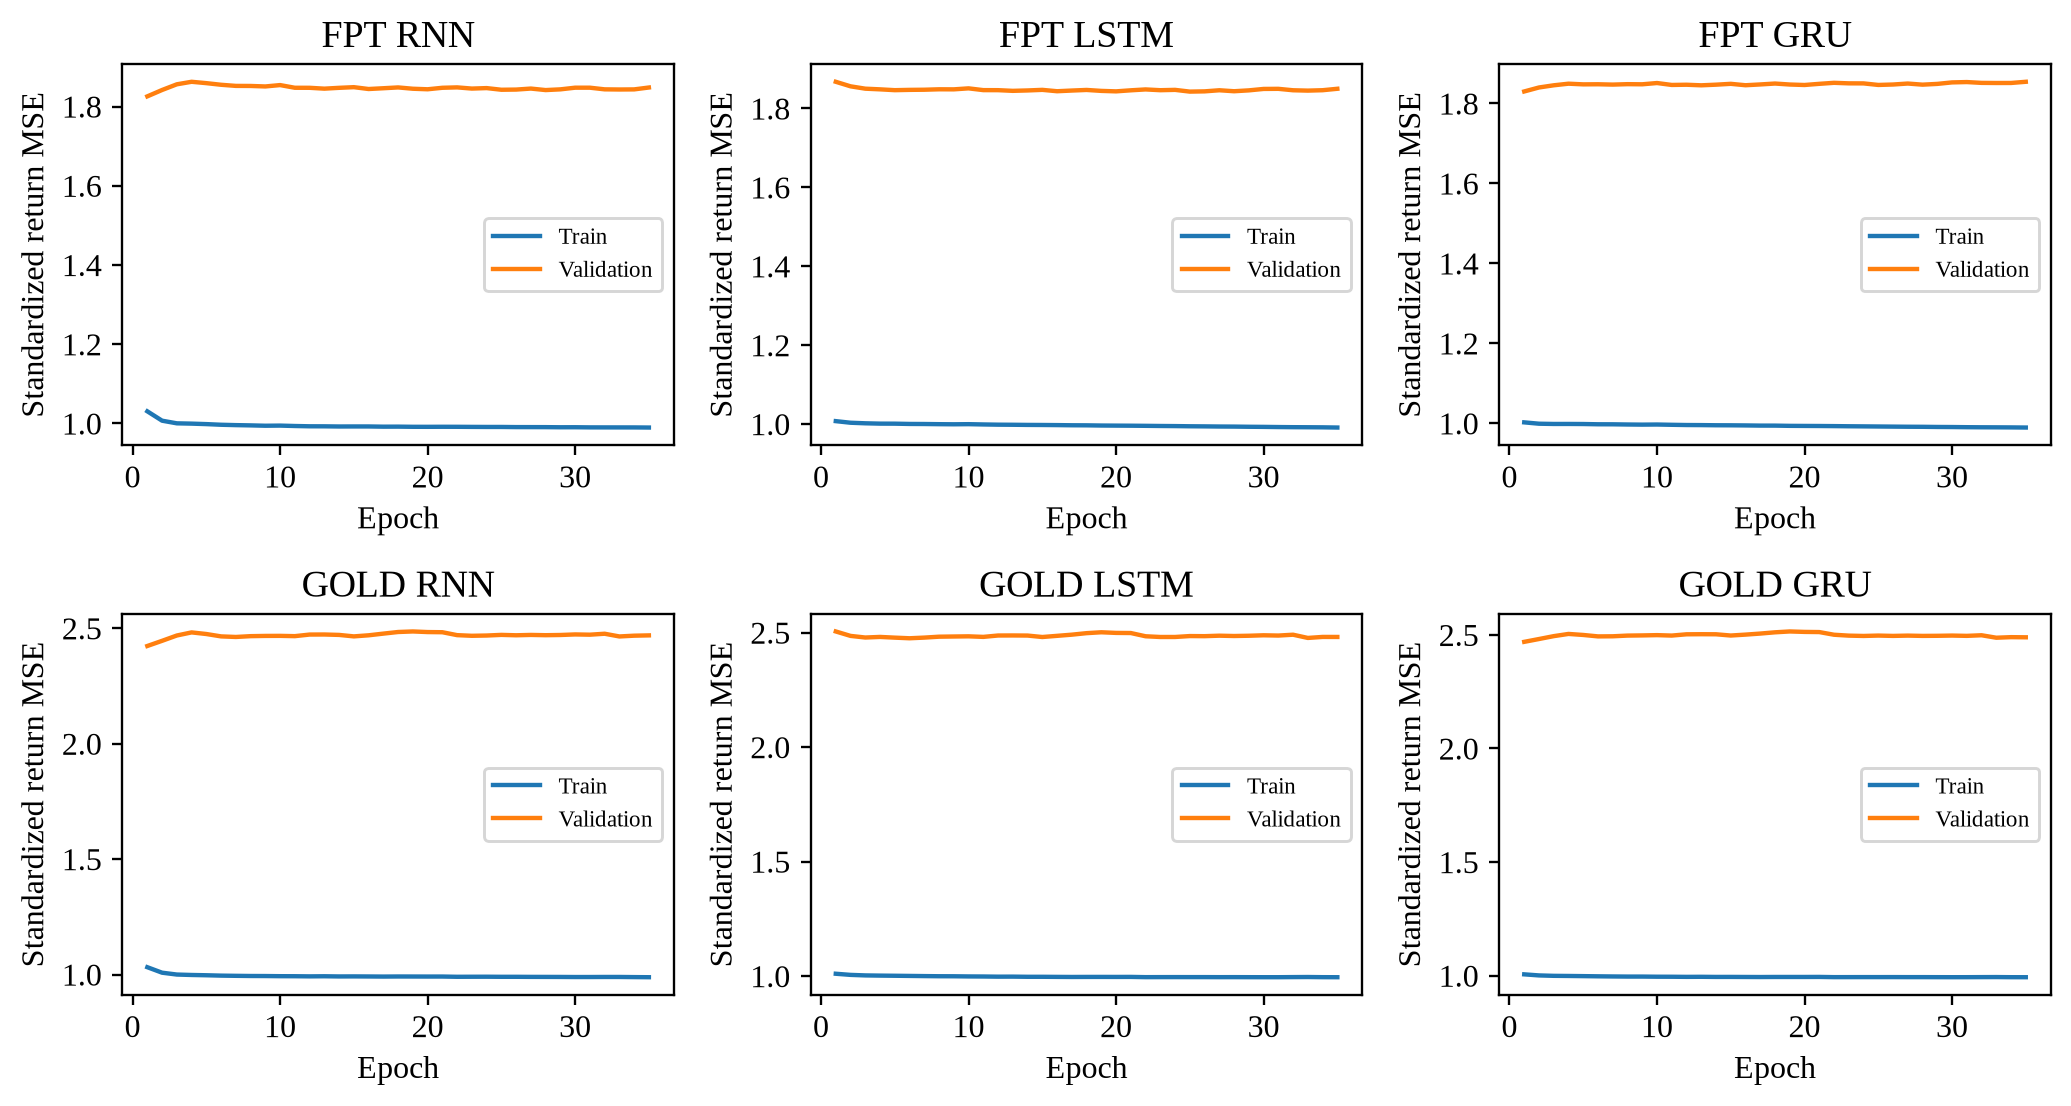
\includegraphics[width=\linewidth,height=.56\textheight,keepaspectratio]{media/media/image21.png}
\caption{Train/validation MSE của sáu mạng trên nhãn log-return đã chuẩn hóa}\label{fig:legacy-4.5}
\end{figure}



Đường học được lưu ở từng epoch, không nội suy thành kết quả chưa chạy.
Loss trong hình là MSE của nhãn chuẩn hóa; MAE trong bảng kết quả là sai
số sau khi đổi về đơn vị giá. Hai thước đo không xếp hạng mô hình giống
nhau trong mọi tình huống. Bởi vậy checkpoint được chọn theo validation
MSE trong từng lần train, còn lựa chọn kiến trúc phục vụ web dùng
validation MAE theo đơn vị gốc, với quy tắc được giữ trước khi xem test.

Mạng có thể học một lợi suất gần 0 và tạo đường giá trông rất sát quan
sát vì mỗi dự báo được neo ở giá của phiên trước. Persistence cũng có
lợi suất dự đoán bằng 0 mà không học tham số. Do đó biểu đồ bám giá chỉ
hỗ trợ quan sát giai đoạn sai lệch; kết luận về độ hữu ích phải dựa trên
phần chênh sai số so với baseline trên cùng ngày nhãn.

\subsection{Chênh lệch so với baseline và độ bất định theo khối}\label{chuxeanh-lux1ec7ch-so-vux1edbi-baseline-vuxe0-ux111ux1ed9-bux1ea5t-ux111ux1ecbnh-theo-khux1ed1i}

\(\Delta_{MAE} = 100\frac{{MAE}_{Persistence} - {MAE}_{model}}{{MAE}_{Persistence}}\)
(4.10)

Giá trị dương của Δ thể hiện giảm MAE so với Persistence. Phân tích bổ
sung lấy mẫu lại các cặp sai số cùng ngày bằng circular block bootstrap,
khối dài 5 quan sát, 2.000 lần và seed 42. Mỗi lần dùng cùng chỉ số cho
mô hình và baseline để giữ tính ghép cặp; lấy theo khối nhằm bảo toàn
một phần phụ thuộc thời gian ngắn. Phân vị 2,5\% và 97,5\% tạo khoảng mô
tả 95\%.

\Needspace{7\baselineskip}
\captionof{table}{Chẩn đoán test so với Persistence; không dùng để đổi lựa chọn web}\label{tab:legacy-4.4}

{\def\LTcaptype{none} % do not increment counter
\begin{longtable}[]{@{}
  >{\raggedright\arraybackslash}p{(\linewidth - 4\tabcolsep) * \real{0.3125}}
  >{\centering\arraybackslash}p{(\linewidth - 4\tabcolsep) * \real{0.2812}}
  >{\centering\arraybackslash}p{(\linewidth - 4\tabcolsep) * \real{0.4062}}@{}}
\toprule\noalign{}
\begin{minipage}[b]{\linewidth}\raggedright
\textbf{Miền / mạng}
\end{minipage} & \begin{minipage}[b]{\linewidth}\centering
\textbf{Giảm MAE (\%)}
\end{minipage} & \begin{minipage}[b]{\linewidth}\centering
\textbf{Khoảng bootstrap 95\%}
\end{minipage} \\
\midrule\noalign{}
\endhead
\bottomrule\noalign{}
\endlastfoot
fpt / RNN & +1.860 & {[}-1.252; +5.105{]} \\
fpt / LSTM & -1.566 & {[}-3.272; -0.110{]} \\
fpt / GRU & -0.381 & {[}-1.087; +0.266{]} \\
gold / RNN & +1.553 & {[}+0.291; +2.732{]} \\
gold / LSTM & -0.164 & {[}-1.676; +1.368{]} \\
gold / GRU & -0.017 & {[}-0.976; +0.926{]} \\
\end{longtable}
}

FPT/RNN có mức giảm điểm khoảng 1,86\% nhưng khoảng bootstrap cắt 0;
FPT/GRU gần baseline và cũng có khoảng cắt 0. Gold/RNN có khoảng dương
trong thiết lập khối đã dùng, song đây là phân tích sau đánh giá, trên
một bản chụp dữ liệu và chưa điều chỉnh cho nhiều so sánh. Không suy rộng thành
bảo đảm vượt baseline ở thị trường tương lai. LSTM FPT kém baseline
trong khoảng mô tả này cũng không chứng minh mọi LSTM đều không phù hợp.

Độ dài khối 5 là lựa chọn phân tích cố định, chưa có nghiên cứu độ nhạy
với khối khác hoặc nhiều seed train. Khoảng trên phản ánh biến thiên khi
lấy mẫu lại các lỗi đã có, không bao gồm toàn bộ bất định do huấn luyện,
thay đổi thị trường hay sai số dữ liệu. Vì vậy nó bổ sung cho điểm MAE
chứ không thay thế walk-forward backtest.

\subsection{Hai demo chuỗi và cách đọc kết quả}\label{hai-demo-chuux1ed7i-vuxe0-cuxe1ch-ux111ux1ecdc-kux1ebft-quux1ea3}

Demo FPT nhận giá gần nhất theo VND và 30 log-return từ cũ đến mới. Mô
hình được cố định là GRU do lựa chọn validation; không thay thành RNN
chỉ vì RNN có test tốt hơn trong lần chạy này. Người dùng có thể thay
một hoặc nhiều lợi suất để xem độ nhạy của mô hình. Đó là phân tích kịch
bản đầu vào, không phải một phép backtest mới và không có kết quả thực
tế để tính sai số ngay trên giao diện.

\productlink{Truy cập sản phẩm thực nghiệm}{https://rag-httm-chatbot.vercel.app/?demo=sequence\#experiments}

Demo vàng chọn GC=F và trả đơn vị USD/oz. Validation chọn Persistence
nên dự báo bằng giá gần nhất dù 30 log-return vẫn có trong form chung.
Giao diện công bố rõ lựa chọn này thay vì gọi một mạng sâu rồi âm thầm
bỏ qua dự đoán của nó. Liên kết dưới mở đúng miền vàng. Cả hai demo đều
báo ngày bản chụp dữ liệu và không gọi API thị trường trực tiếp để tự làm mới
giá.

\productlink{Truy cập sản phẩm thực nghiệm}{https://rag-httm-chatbot.vercel.app/?demo=sequence&domain=gold\#experiments}

Bộ phân tích đầu vào được sửa để không chuyển một phần tử trống giữa hai
dấu phẩy thành số 0. Máy chủ vẫn yêu cầu đúng 30 số hữu hạn trong
{[}−1,1{]} và giá gần nhất dương. Các giới hạn này kiểm tra cấu trúc yêu
cầu, không chứng minh kịch bản nằm trong phân phối train. Không dùng giá
trị đầu ra để suy ra lợi nhuận, tín hiệu mua bán hoặc mức rủi ro đầu tư
cá nhân.

\section{Hạn chế và khả năng mở rộng}\label{hux1ea1n-chux1ebf-vuxe0-khux1ea3-nux103ng-mux1edf-rux1ed9ng}

Thực nghiệm là dự báo một bước trên bản chụp dữ liệu cố định, không phải dự báo
nhiều bước tương lai hoặc dữ liệu trực tiếp. Phân tích bootstrap theo
khối ở trên chưa thay thế kiểm tra nhiều seed và walk-forward backtest.
Hướng mở rộng gồm nghiên cứu độ nhạy với chiều dài cửa sổ, các biến đầu
vào có timestamp và ngân sách tuning khóa trước. Không dùng test lặp lại
để điều chỉnh cấu hình.

Mô hình triển khai giữ checkpoint train lịch sử, không refit bằng test
để giữ được dấu vết đánh giá. Người dùng có thể sửa giá gần nhất và 30
log-return để thử kịch bản; kết quả không có khoảng tin cậy đã hiệu
chỉnh cho kịch bản ngoài miền. Checkpoint của mọi RNN/LSTM/GRU và
training history được lưu riêng để kiểm tra.

\part{Biểu diễn tri thức và hệ đa agent}
\chapter{Knowledge graph và RAG}\label{chux1b0ux1a1ng-5.-knowledge-graph-vuxe0-RAG}

Dự đoán số hoặc nhãn mới giải quyết một phần nhu cầu của người dùng. Khi
hỏi giá gần nhất đi cùng chỉ báo nào, hoặc một khái niệm sức khỏe có
liên hệ với yếu tố nào, người dùng còn cần ngữ cảnh và bằng chứng. Một
mô hình dự đoán không tự trở thành kho tri thức, còn câu trả lời trôi
chảy không bảo đảm có căn cứ.

Chương tổ chức tri thức dưới hai dạng bổ trợ: văn bản có thể truy xuất
theo mức liên quan và đồ thị thực thể--quan hệ có thể kiểm tra đường
nối. Prototype sử dụng TF-IDF, NetworkX và bộ tổng hợp xác định; giao
diện sức khỏe dùng BM25 cùng luật đối thoại. Phạm vi này cho phép quan
sát luồng bằng chứng mà không gán cho hệ thống năng lực của một mô hình
ngôn ngữ chưa được tích hợp.

Từ nền tảng KG và RAG, chương chuyển sang dữ liệu ba miền, các bài toán
dự đoán, cơ chế truy xuất, giao diện và kiểm thử triển khai. Phần phân
tích bổ sung theo dõi một câu hỏi cụ thể qua thứ hạng tài liệu, quan hệ
đồ thị và câu trả lời, đồng thời tách rõ điểm truy xuất khỏi chất lượng
suy luận.

\section{Mở đầu}\label{mux1edf-ux111ux1ea7u}

Knowledge Graph (KG) và Retrieval-Augmented Generation (RAG) xuất phát
từ hai truyền thống khác nhau. KG nhấn mạnh biểu diễn tường minh: thực
thể nào tồn tại, chúng liên hệ ra sao và ràng buộc nào phải được giữ.
RAG xuất phát từ nhu cầu cho mô hình sinh tiếp cận một kho tri thức
ngoài tại thời điểm trả lời. Khi ghép hai hướng này, hệ thống vừa có khả
năng tìm kiếm mềm theo ngôn ngữ, vừa có cấu trúc để kiểm tra đường suy
luận.

Bài làm lựa chọn kiến trúc có thể chạy trọn trong một notebook. TF-IDF
đảm nhiệm truy xuất văn bản, NetworkX lưu đồ thị, còn bộ tổng hợp ghép
bằng chứng tìm được thành câu trả lời. Dữ liệu FPT.VN và GC=F được đọc
từ bản chụp dữ liệu đã khóa trong lần tái lập; có chế độ tải mới khi được bật;
dữ liệu tiểu đường lấy từ scikit-learn.

Ba miền được chọn tạo ra phép thử đủ khác biệt. Y tế yêu cầu diễn đạt
thận trọng; chứng khoán là chuỗi thời gian nội địa; vàng chịu tác động
của yếu tố vĩ mô và được niêm yết quốc tế. Một pipeline dùng chung phải
giữ được ngữ cảnh riêng của từng miền mà không trộn lẫn bằng chứng.

\begin{figure}[H]
\centering
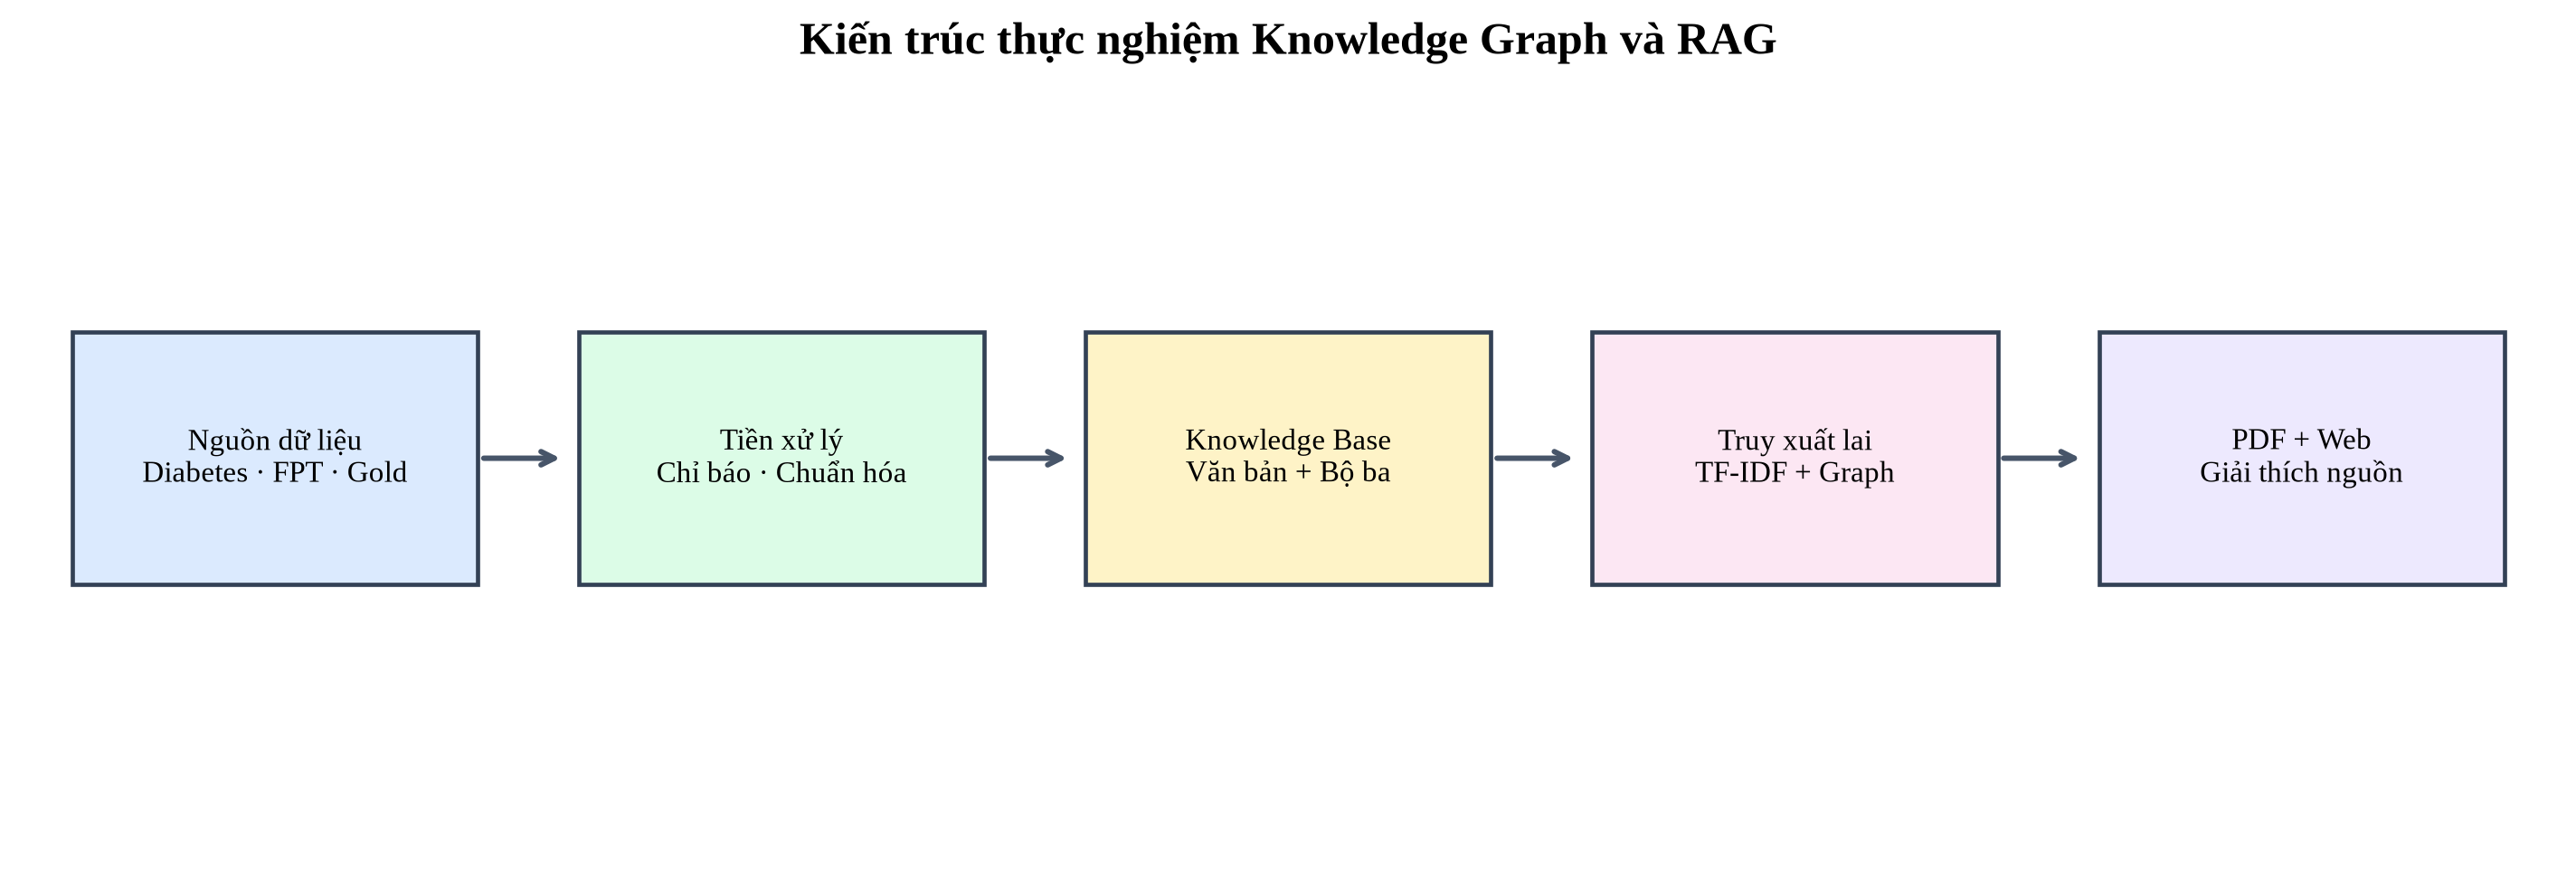
\includegraphics[width=\linewidth,height=.56\textheight,keepaspectratio]{media/media/image22.png}
\caption{Kiến trúc KG và RAG}\label{fig:legacy-5.1}
\end{figure}



\subsection{Lịch sử phát triển của knowledge graph}\label{lux1ecbch-sux1eed-phuxe1t-triux1ec3n-cux1ee7a-knowledge-graph}

Ý tưởng nối các khái niệm thành mạng ngữ nghĩa đã xuất hiện từ những
nghiên cứu ban đầu về trí nhớ và biểu diễn tri thức. Sau đó, hệ chuyên
gia đưa luật IF-THEN vào các miền hẹp. Bước ngoặt của Web ngữ nghĩa là
việc chuẩn hóa RDF, RDFS, OWL và SPARQL, khiến bộ ba chủ thể-vị từ-đối
tượng trở thành một ngôn ngữ trao đổi máy đọc được,.

Năm 2012, cách gọi Knowledge Graph được phổ biến rộng rãi qua công cụ
tìm kiếm của Google. Trong doanh nghiệp, KG tiếp tục được dùng cho danh
mục sản phẩm, phát hiện gian lận, quản trị dữ liệu chủ và gợi ý nội
dung. Điểm chung không phải một loại cơ sở dữ liệu cụ thể, mà là cách
coi quan hệ giữa các thực thể là công dân hạng nhất.

Ở bài này, đồ thị được cài bằng Labeled Property Graph đơn giản. Mỗi nút
có type và domain; mỗi cạnh có nhãn quan hệ. Lựa chọn này gần với cách
Neo4j tổ chức dữ liệu và thuận tiện cho trực quan hóa, dù chưa khai thác
đầy đủ suy luận ontology như OWL.

\subsection{Lịch sử phát triển của RAG}\label{lux1ecbch-sux1eed-phuxe1t-triux1ec3n-cux1ee7a-RAG}

Trước RAG, các hệ hỏi đáp mở thường tách bộ tìm kiếm tài liệu và bộ đọc
hiểu. REALM đưa cơ chế truy xuất vào quá trình tiền huấn luyện. Lewis và
cộng sự sau đó định danh kiến trúc Retrieval-Augmented Generation, kết
hợp bộ truy xuất dense với mô hình sinh seq2seq cho nhiệm vụ giàu tri
thức.

Sự phổ biến của mô hình ngôn ngữ lớn khiến RAG trở thành một mẫu triển
khai thực dụng: tài liệu có thể cập nhật mà không cần huấn luyện lại
toàn bộ mô hình, đồng thời câu trả lời giữ được liên kết về nguồn. Tuy
nhiên, vector search thường ưu tiên đoạn giống câu hỏi và có thể bỏ qua
quan hệ gián tiếp. GraphRAG giải quyết phần thiếu này bằng việc xây thực
thể, quan hệ, cụm và tóm tắt theo cấu trúc.

Nguyên mẫu trong notebook không cố tái tạo toàn bộ Microsoft GraphRAG.
Nó giữ hai ý cốt lõi: truy xuất đồng thời từ văn bản và đồ thị, sau đó
đưa cả hai nhóm bằng chứng vào bước tổng hợp.

\subsection{Vai trò và ý nghĩa trong AI}\label{vai-truxf2-vuxe0-uxfd-nghux129a-trong-ai}

KG giúp mô hình có từ điển thực thể thống nhất, quan hệ có tên và đường
đi có thể kiểm tra. RAG giúp tri thức ngoài đi vào ngữ cảnh trả lời đúng
thời điểm. Kết hợp hai thành phần làm giảm nguy cơ câu trả lời chỉ dựa
trên tương đồng bề mặt, nhưng không đồng nghĩa loại bỏ hoàn toàn sai
sót.

Trong y tế, giá trị quan trọng nhất là provenance: người đọc phải biết
nhận xét dựa trên biến nào và nguồn nào. Trong tài chính, dữ liệu có
tính thời điểm nên ngày quan sát phải đi cùng con số. Trong cả hai
trường hợp, câu trả lời nên phân biệt sự kiện đo được, quan hệ thường
gặp và kết luận mang tính dự báo.

Ý nghĩa học thuật của bài nằm ở khả năng chạy lại. Người chấm có thể Run
All, xem dữ liệu thô đã lưu, đối chiếu bộ ba, kiểm tra tài liệu được
truy xuất và mở PDF được sinh từ cùng một trạng thái chạy.

\subsection{Phạm vi, câu hỏi và đóng góp}\label{phux1ea1m-vi-cuxe2u-hux1ecfi-vuxe0-ux111uxf3ng-guxf3p}

Bài đặt ba câu hỏi: (1) một cấu trúc KG thống nhất có mô tả được ba miền
khác nhau không; (2) truy xuất lai có cung cấp nhiều bằng chứng hơn
vector search đơn lẻ không; và (3) có thể đóng gói toàn bộ quy trình
trong một notebook duy nhất không.

Đóng góp thực hành gồm lớp KnowledgeGraphCore, bộ tải Yahoo Finance
không cần API key, các bước tạo chỉ báo, VectorRetriever, truy xuất đồ
thị theo miền, đánh giá precision@3, ứng dụng dự đoán, chatbot sức khỏe
có nguồn và bộ sinh PDF. Mọi tệp phụ đều được tạo lại từ notebook.

Ba nguồn dữ liệu được mô tả bằng số dòng, số cột, khoảng thời gian, đơn
vị và biến đích. Bảng được sinh trực tiếp từ DataFrame sau xử lý nên
khớp với lần chạy hiện tại.

\begin{figure}[H]
\centering
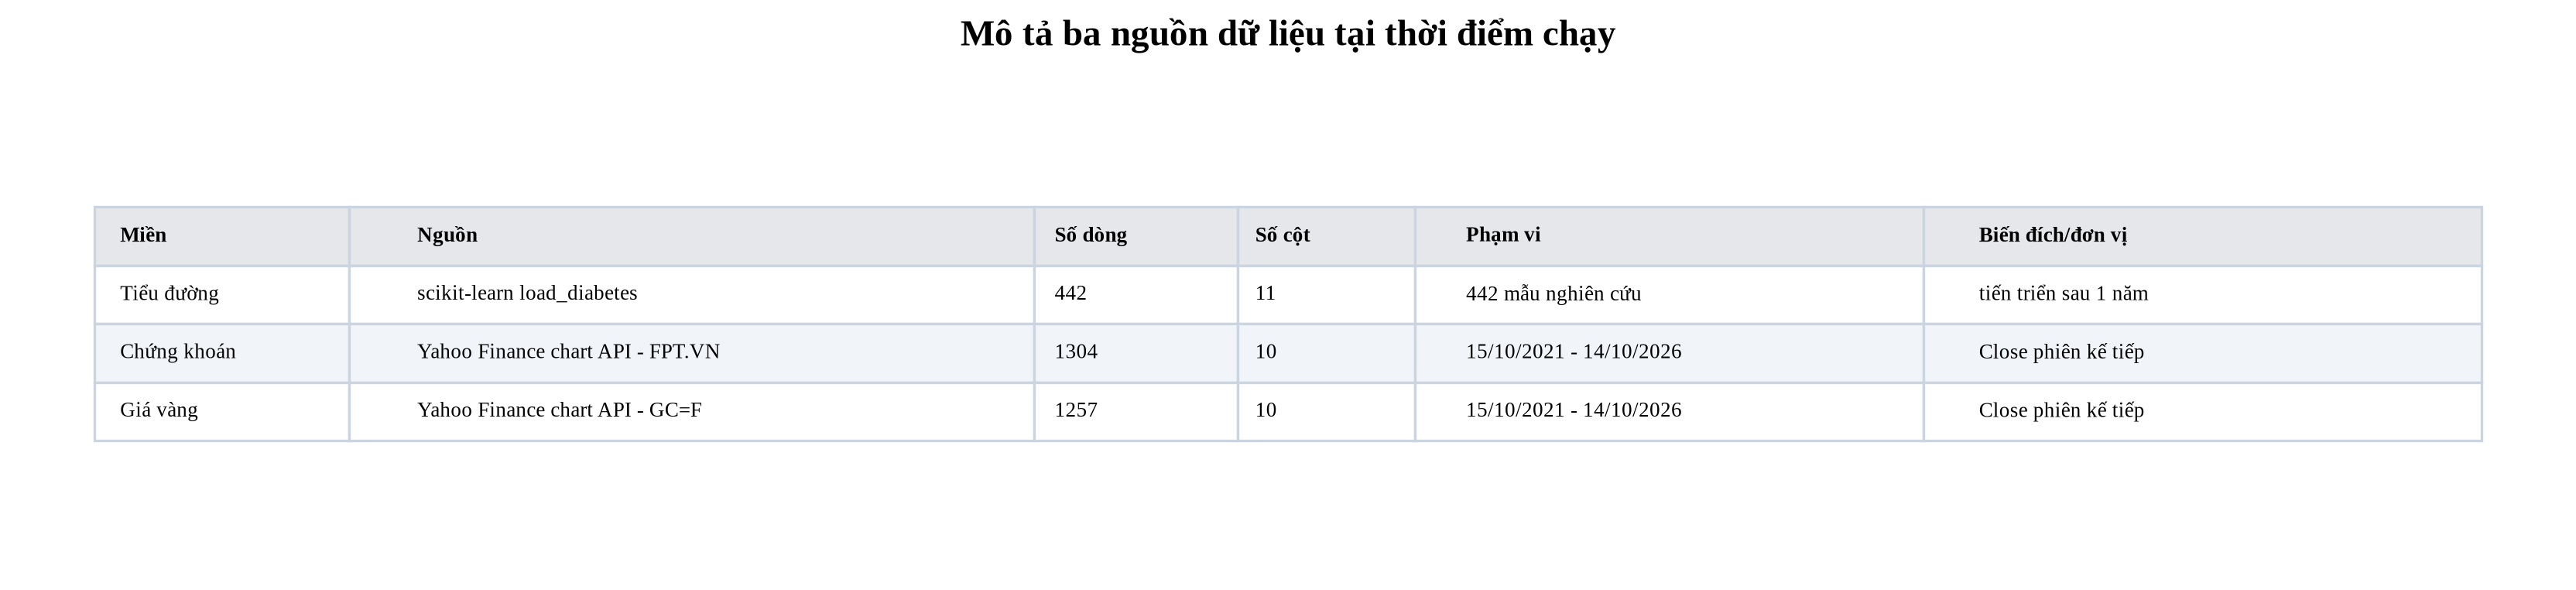
\includegraphics[width=\linewidth,height=.56\textheight,keepaspectratio]{media/media/image23.png}
\caption{Thông tin ba miền dữ liệu}\label{fig:legacy-5.2}
\end{figure}



\section{Knowledge graph - knowledge base}\label{knowledge-graph---knowledge-base}

Knowledge Base trong bài gồm hai lớp. Lớp văn bản giữ các đoạn mô tả dữ
liệu, phương pháp và kết quả theo từng miền. Lớp đồ thị giữ thực thể
cùng các quan hệ có hướng. Hai lớp dùng chung nhãn domain để ngăn truy
xuất nhầm giữa tiểu đường, cổ phiếu và vàng.

Đồ thị tại lần chạy này có 25 nút và 22 cạnh. Kích thước nhỏ giúp người
đọc kiểm tra thủ công. Khi mở rộng, cùng schema có thể chuyển sang Neo4j
hoặc một triple store mà không thay đổi ý nghĩa bộ ba.

Knowledge Base không chỉ chứa kiến thức tĩnh. Các nút quan sát như giá
FPT hoặc giá vàng gần nhất được tạo từ dữ liệu tải về. Cách làm này nối
câu trả lời với đúng trạng thái thị trường tại thời điểm chạy.

\begin{figure}[H]
\centering
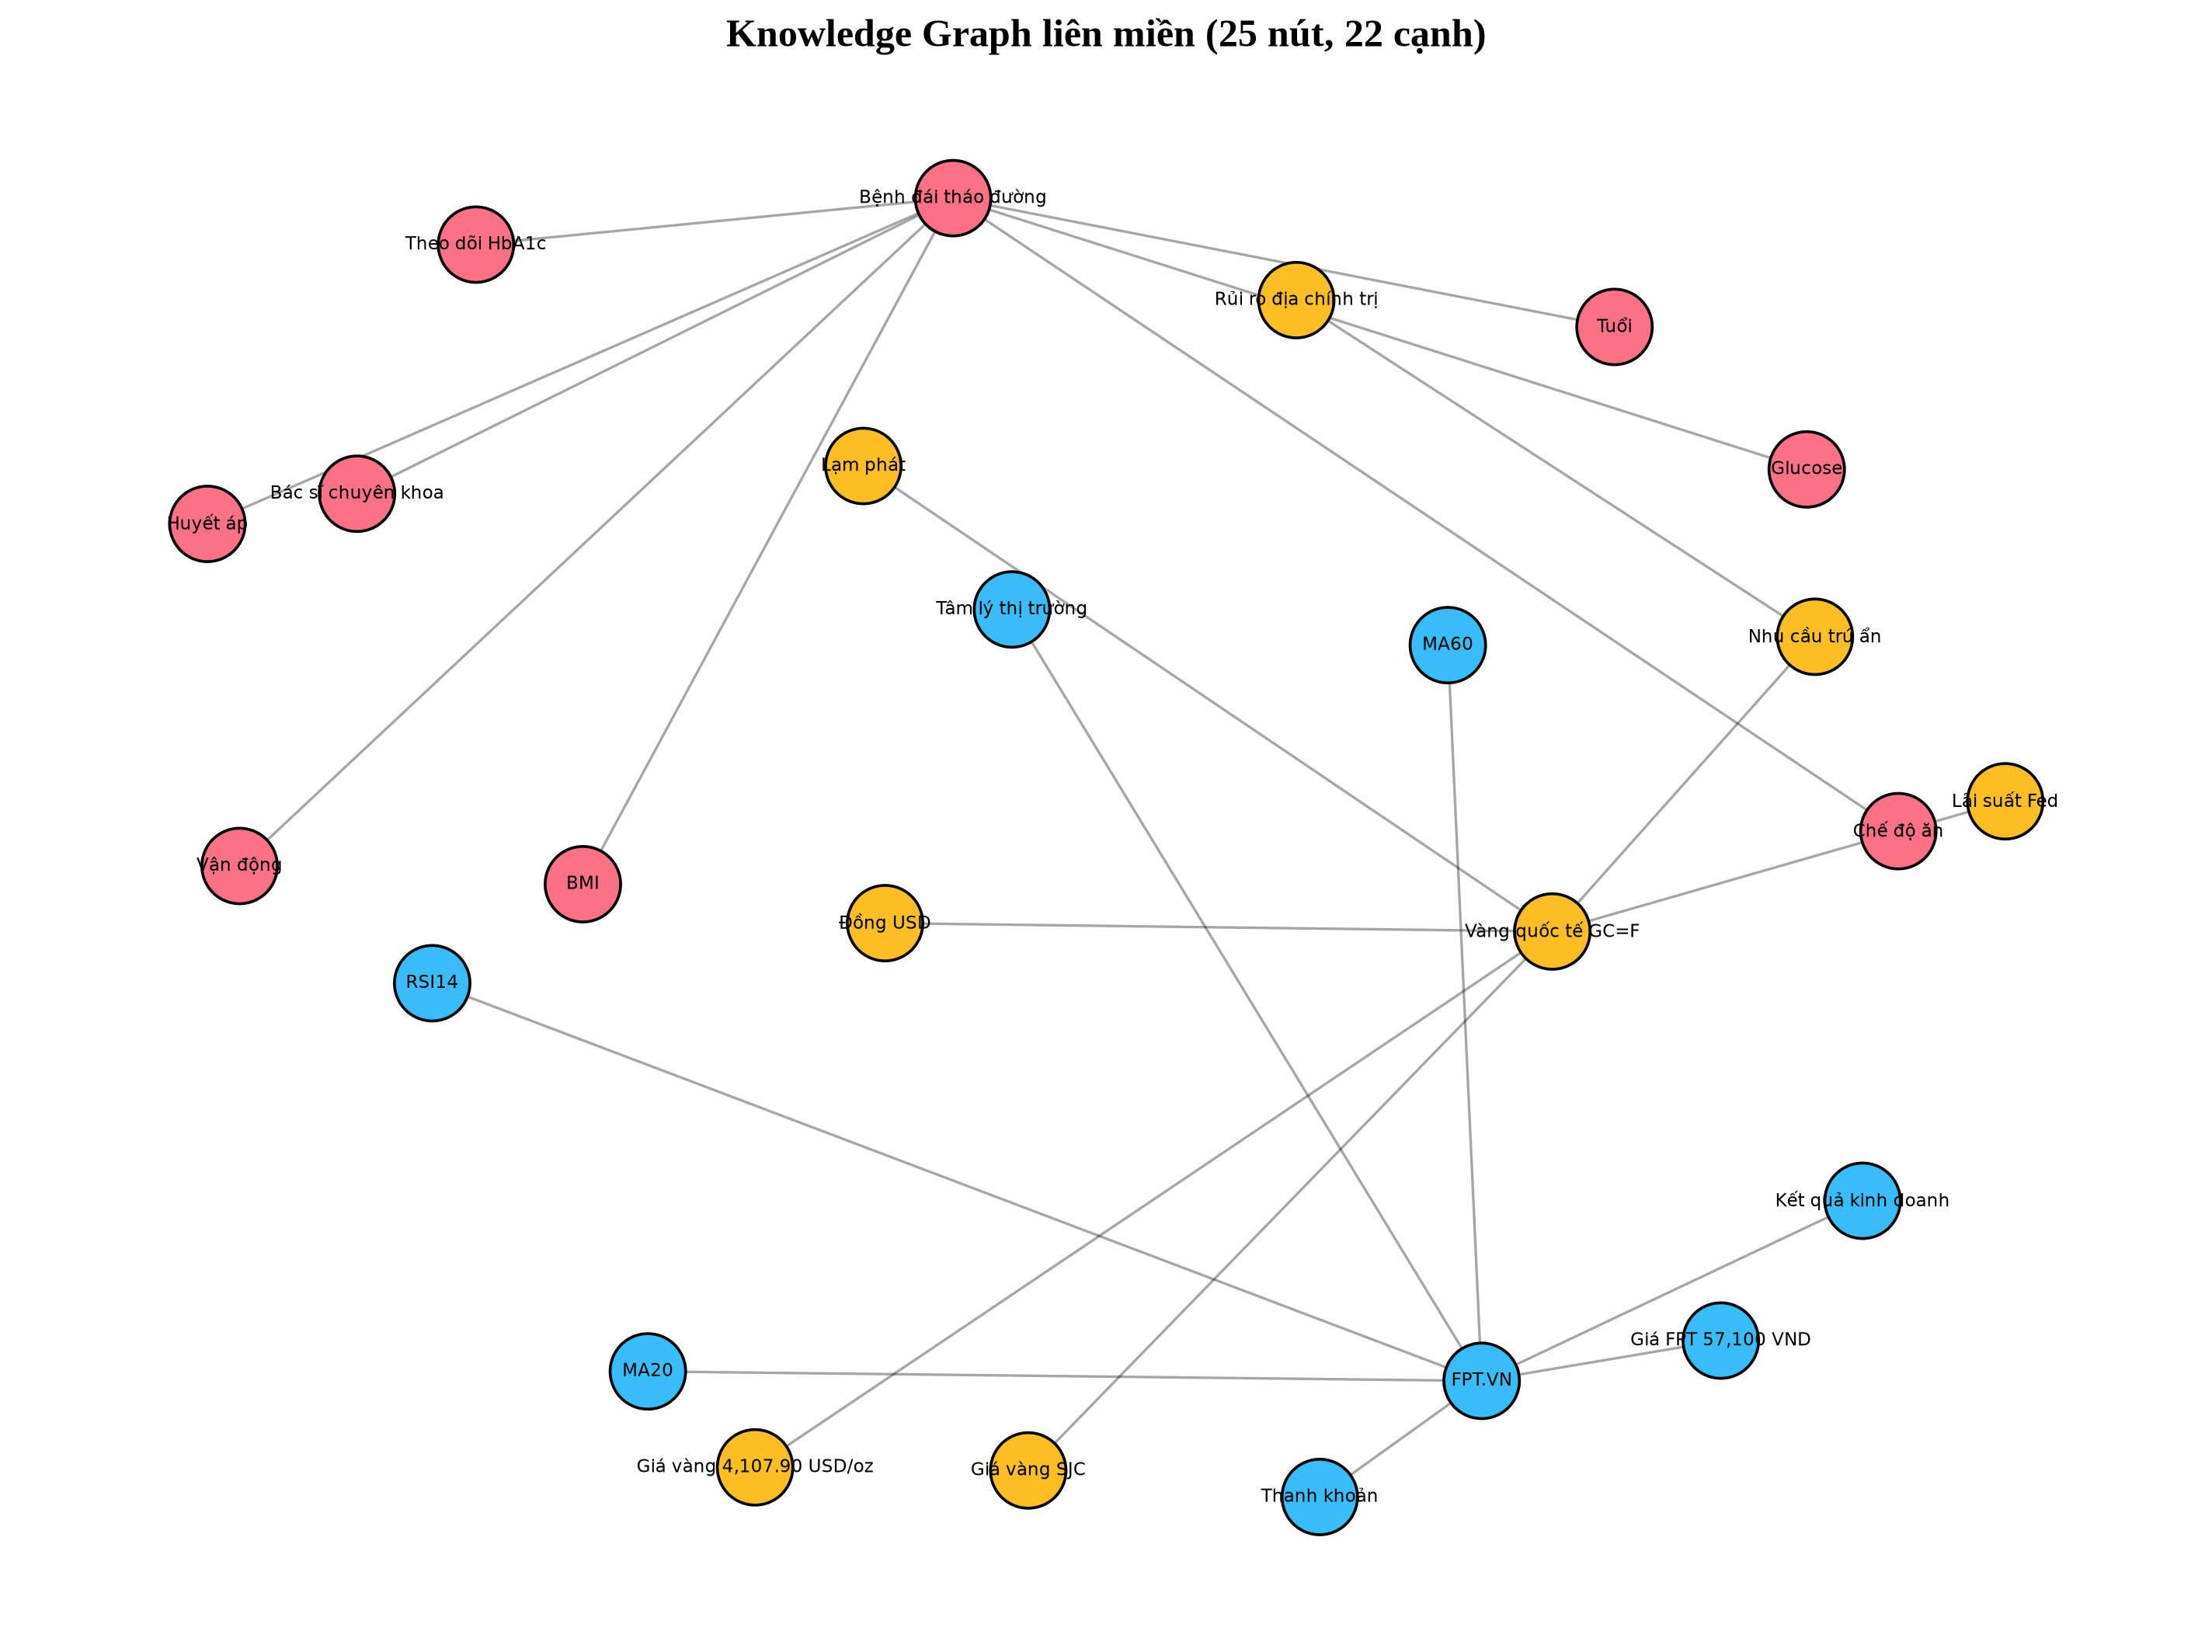
\includegraphics[width=\linewidth,height=.56\textheight,keepaspectratio]{media/media/image24.png}
\caption{Đồ thị tri thức đa miền}\label{fig:legacy-5.3}
\end{figure}



\subsection{Bộ ba, thực thể và quan hệ}\label{bux1ed9-ba-thux1ef1c-thux1ec3-vuxe0-quan-hux1ec7}

Một bộ ba có dạng (s, p, o), trong đó s là thực thể nguồn, p là quan hệ
có tên và o là thực thể hoặc giá trị đích. Ví dụ: (MA20,
MÔ\_TẢ\_XU\_HƯỚNG\_NGẮN\_HẠN\_CỦA, FPT.VN). Bộ ba này không khẳng định
xu hướng sẽ tiếp diễn; nó chỉ diễn tả vai trò của chỉ báo.

Thực thể được gắn type như Condition, Biomarker, Stock,
TechnicalIndicator, Commodity hoặc MacroFactor. Thuộc tính domain tách
ba không gian nghiệp vụ. Tên quan hệ dùng động từ viết hoa để người đọc
có thể đọc thành câu.

Việc chọn quan hệ là công đoạn có tính chủ quan. Báo cáo ưu tiên từ
CÓ\_THỂ\_TÁC\_ĐỘNG hoặc CÓ\_QUAN\_HỆ... thay vì GÂY\_RA khi dữ liệu
không đủ để chứng minh nhân quả.

\subsection{Knowledge graph core engine}\label{knowledge-graph-core-engine}

Lớp KnowledgeGraphCore bọc MultiDiGraph của NetworkX. add\_entity quản
lý nút và thuộc tính; add\_relation thêm cạnh có hướng; neighbors trả về
bằng chứng một bước; multi\_hop tìm các đường đơn trong giới hạn số hop.
Cấu trúc MultiDiGraph cho phép hai thực thể có nhiều loại quan hệ.

Độ phức tạp của truy vấn lân cận tỷ lệ với bậc của nút. Truy vấn mọi
đường đơn có thể tăng nhanh theo kích thước đồ thị, vì vậy max\_hops
phải được giới hạn. Với đồ thị sản xuất, cần chỉ mục, phân quyền và
chiến lược truy vấn cụ thể thay vì duyệt toàn bộ.

Toàn bộ cạnh được xuất thành knowledge\_graph\_triples.csv. Đây là điểm
kiểm tra thuận tiện: mỗi dòng trong tệp phải đọc được như một phát biểu,
không có nút mồ côi vô nghĩa và không chứa con số không rõ ngày.

\begin{figure}[H]
\centering
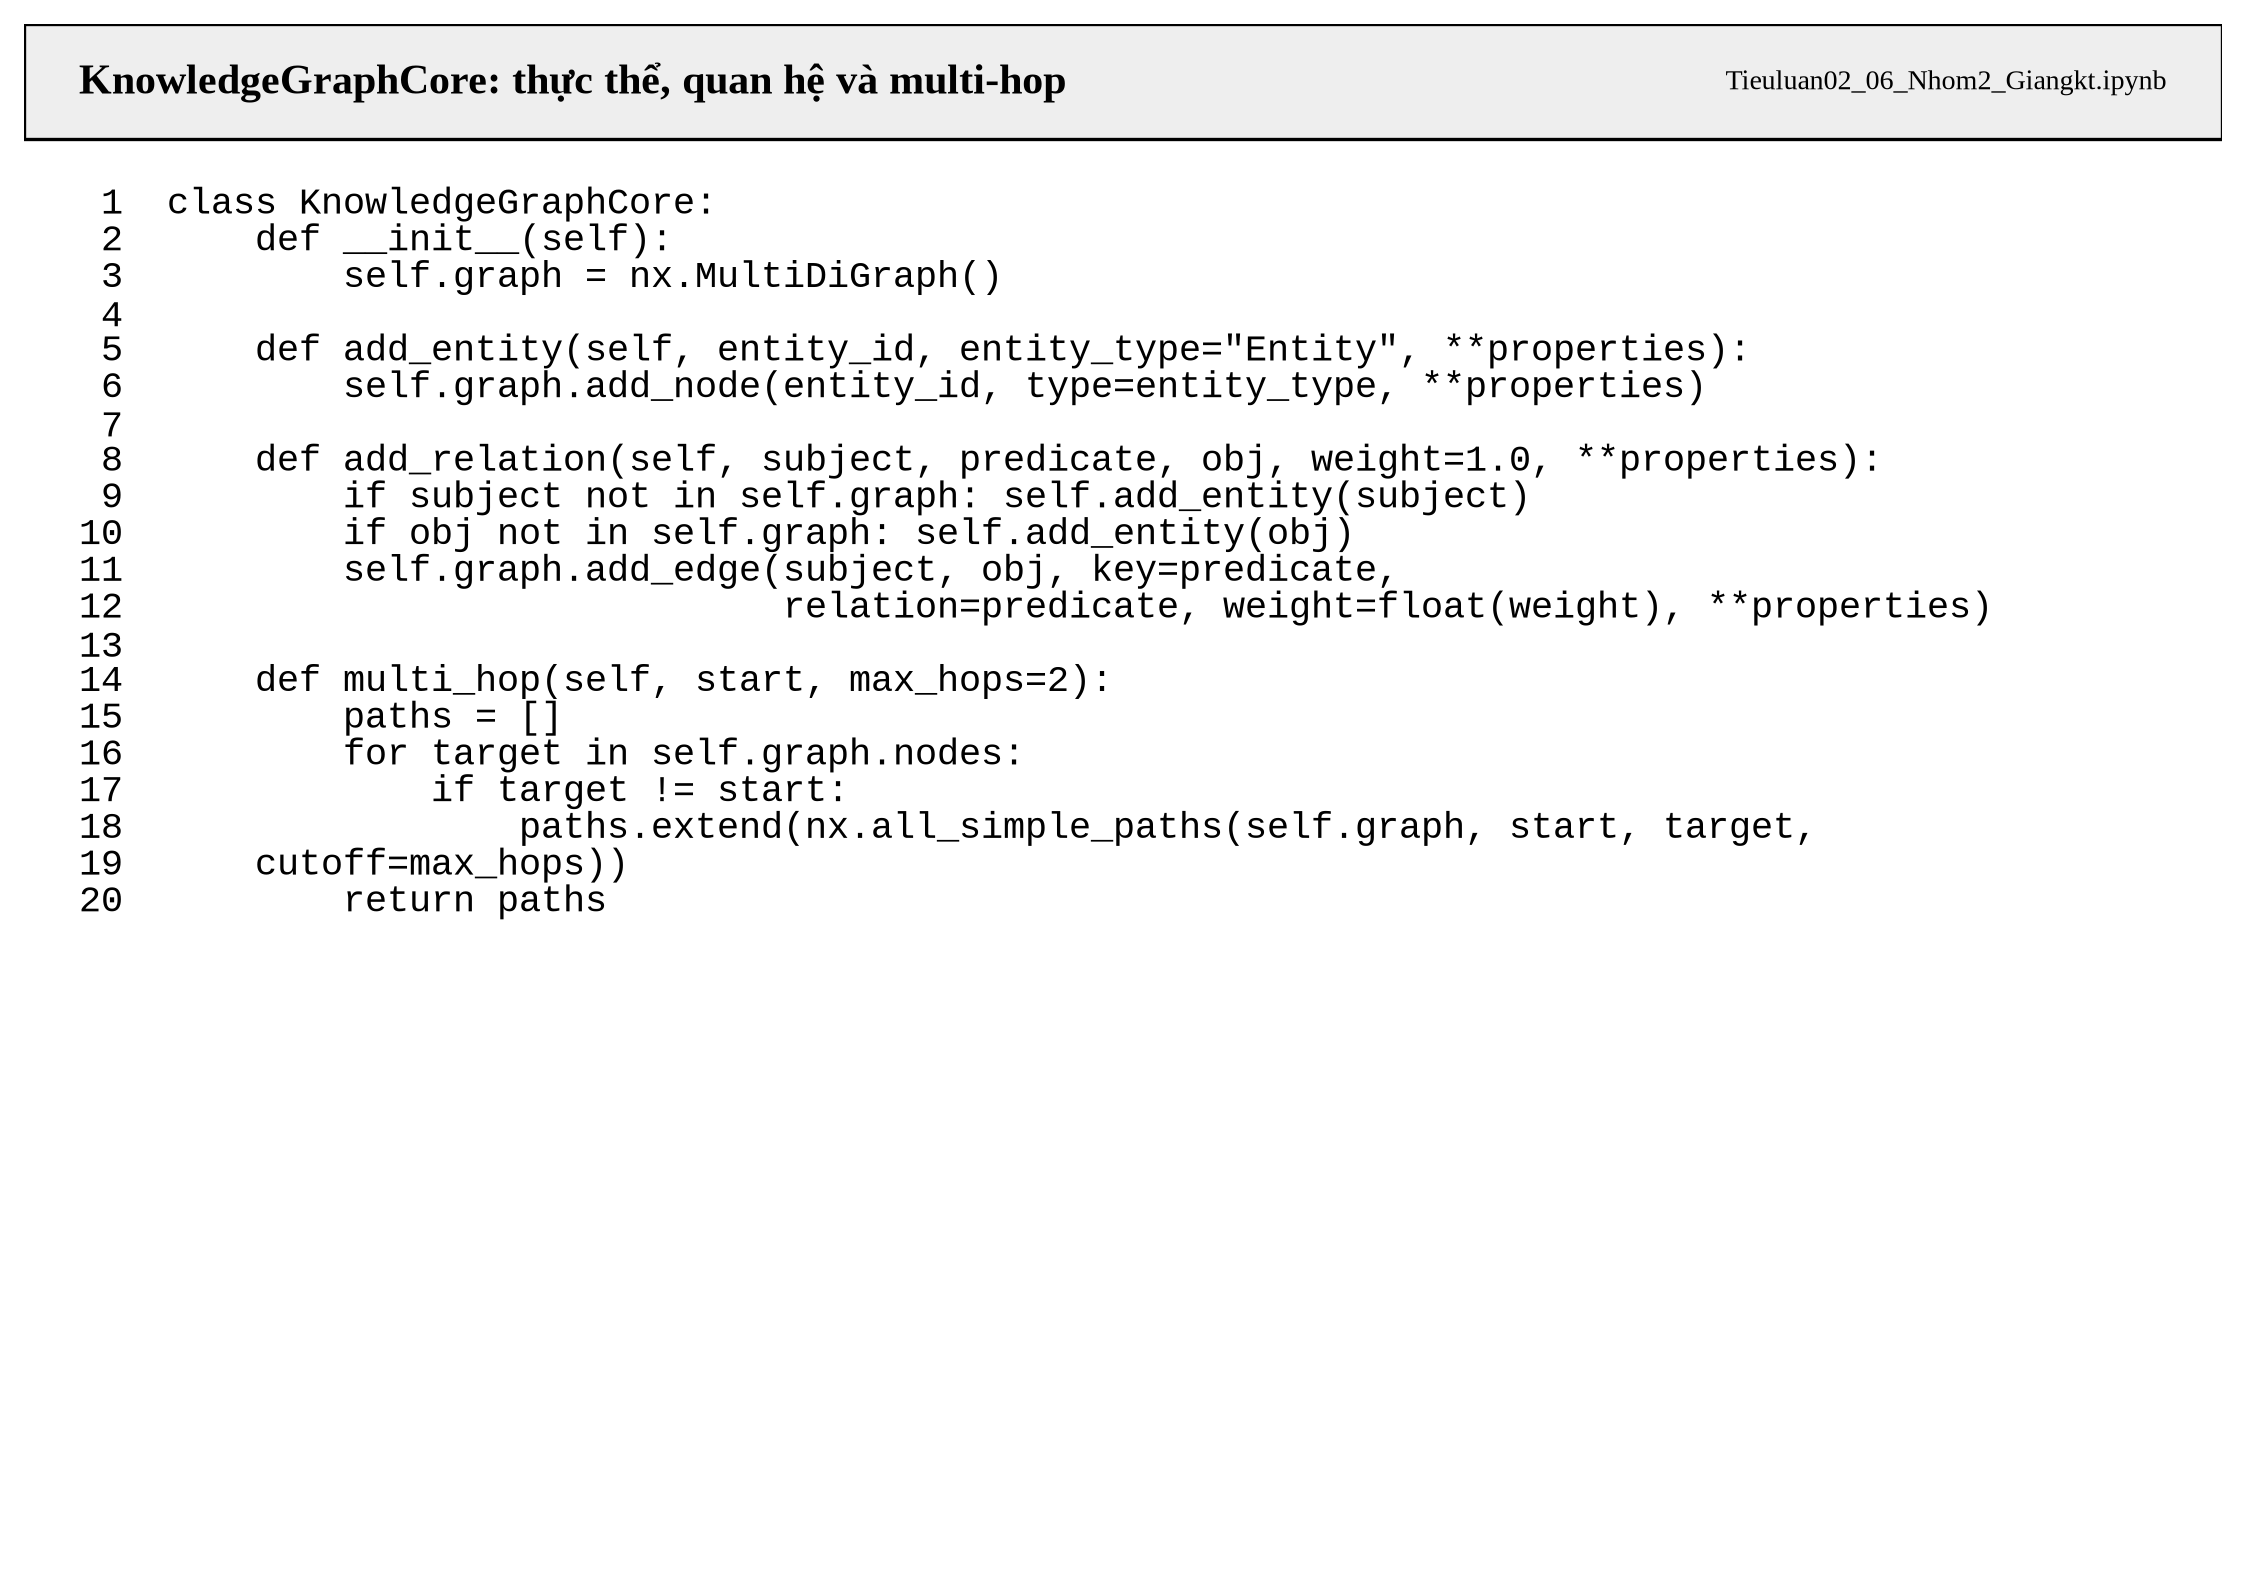
\includegraphics[width=\linewidth,height=.56\textheight,keepaspectratio]{media/media/image25.png}
\caption{Cấu trúc KnowledgeGraphCore}\label{fig:legacy-5.4}
\end{figure}



\subsection{Rdf và labeled property graph}\label{rdf-vuxe0-labeled-property-graph}

RDF phù hợp khi cần URI toàn cục, liên kết dữ liệu và suy luận theo
chuẩn W3C. Labeled Property Graph thuận tiện khi cạnh cần thuộc tính và
truy vấn đường đi là trọng tâm. Bài chọn mô hình thứ hai vì mục tiêu là
nguyên mẫu phân tích và trực quan hóa bằng Python.

Nếu chuyển sang RDF, các entity\_id cần ánh xạ thành IRI; relation thành
predicate; giá trị số thành literal có datatype. Nếu chuyển sang Neo4j,
type có thể thành node label, relation thành relationship type và các
trường domain/source thành property.

Không có mô hình nào tốt tuyệt đối. Tiêu chí chọn là khả năng tích hợp
với hệ thống, yêu cầu suy luận, quy mô và kỹ năng vận hành của nhóm.

\subsection{Chất lượng và quản trị tri thức}\label{chux1ea5t-lux1b0ux1ee3ng-vuxe0-quux1ea3n-trux1ecb-tri-thux1ee9c}

Một KG hữu ích cần hơn số lượng cạnh. Bốn kiểm tra tối thiểu gồm: tính
duy nhất của định danh, tính hợp lệ của miền-phạm vi, nguồn gốc quan hệ
và thời hạn của dữ liệu động. Các quan hệ y tế và tài chính phải có mức
tin cậy hoặc câu chữ thể hiện độ bất định.

Bài hiện lưu source ở lớp tài liệu và domain ở lớp đồ thị. Bản sản xuất
nên bổ sung created\_at, valid\_from, valid\_to, confidence và
evidence\_id cho từng cạnh. Khi đó, một quan hệ đã cũ có thể bị loại
trước khi đưa vào prompt.

Kiểm soát chất lượng cần vòng phản hồi của chuyên gia. Bác sĩ xác nhận
ontology y tế; chuyên viên tài chính rà soát khái niệm và đơn vị; kỹ sư
dữ liệu kiểm tra schema cùng pipeline cập nhật.

\section{RAG - retrieval-augmented generation}\label{RAG---retrieval-augmented-generation}

Pipeline RAG gồm ingestion, indexing, retrieval và generation. Văn bản
được chia thành các đơn vị có nguồn; TF-IDF biến chúng thành vector;
cosine similarity xếp hạng theo câu hỏi. Bước sinh ghép hai đoạn phù hợp
nhất với các bộ ba liên quan.

TF-IDF được chọn vì minh bạch, nhẹ và tái lập. Hạn chế là không hiểu
đồng nghĩa sâu như embedding. Để giảm nhược điểm, câu hỏi được nhận diện
miền bằng một từ điển alias và GraphRAG bổ sung các quan hệ từ đồ thị.

Mỗi câu trả lời trả về cả documents, score, triples và domain. Cấu trúc
này quan trọng hơn phần câu chữ: giao diện hoặc báo cáo có thể trình bày
bằng chứng mà không phải phân tích ngược chuỗi văn bản.

\begin{figure}[H]
\centering
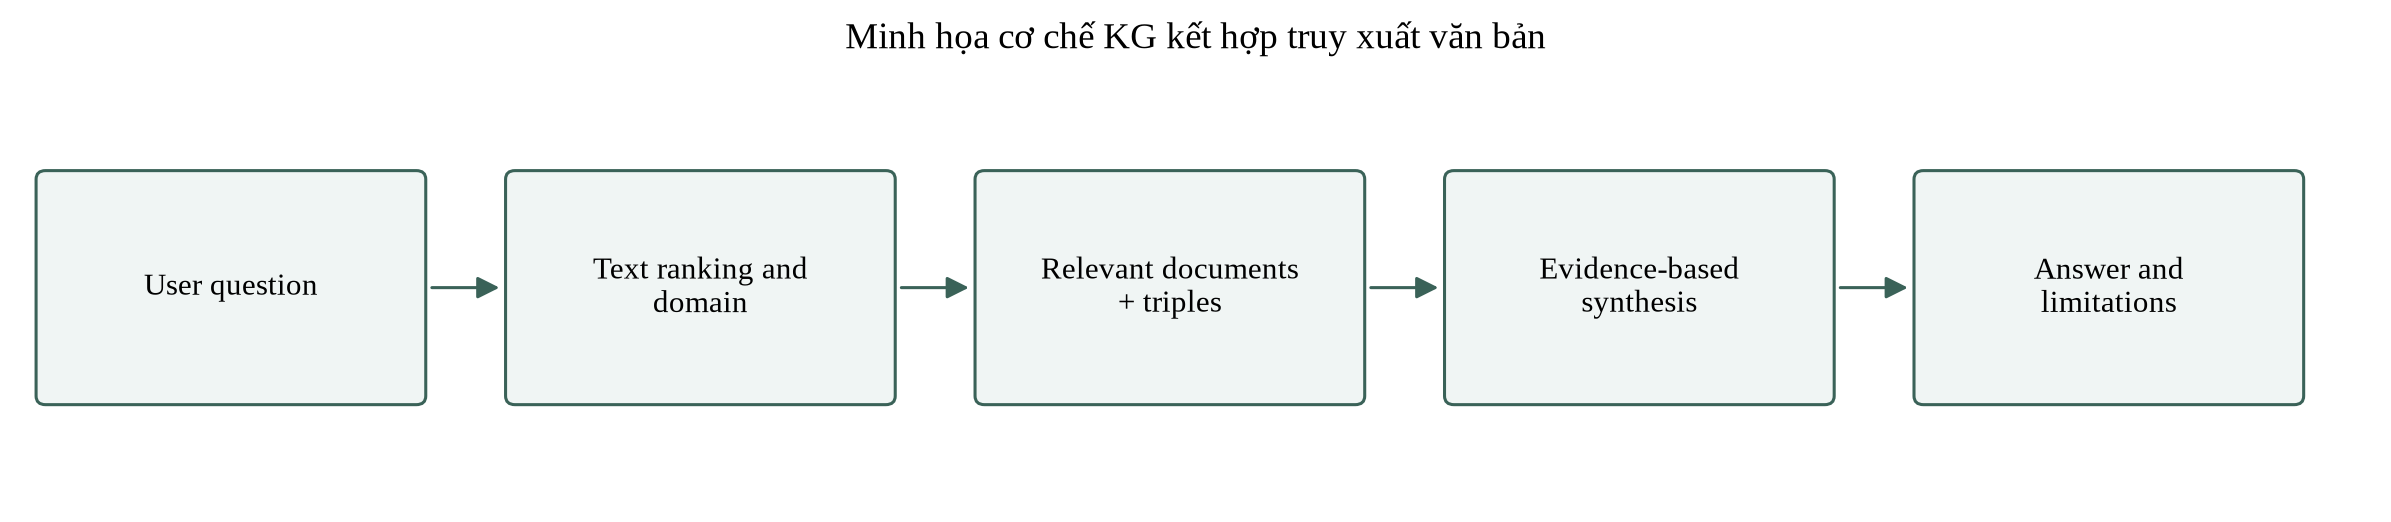
\includegraphics[width=\linewidth,height=.56\textheight,keepaspectratio]{media/media/image26.png}
\caption{Minh họa luồng truy xuất và tổng hợp bằng chứng}\label{fig:legacy-5.5}
\end{figure}



\subsection{Nạp, lập chỉ mục và truy xuất}\label{nux1ea1p-lux1eadp-chux1ec9-mux1ee5c-vuxe0-truy-xuux1ea5t}

Các tài liệu ngắn được xây từ mô tả bộ dữ liệu và kết quả thực nghiệm.
Trong hệ thống lớn, ingestion cần đọc PDF, HTML hoặc cơ sở dữ liệu;
chuẩn hóa Unicode; bỏ trùng; chia đoạn theo ngữ nghĩa; và gắn metadata
trước khi embedding.

TfidfVectorizer dùng unigram và bigram. Bigram giúp phân biệt các cụm
như giá vàng, tiểu đường, lãi suất Fed. top\_k=3 giữ ngữ cảnh ngắn và dễ
kiểm tra. Precision@3 theo domain được dùng như phép đo đơn giản cho độ
đúng của truy xuất.

Điểm cosine chỉ phản ánh độ gần từ vựng, không phải độ đúng. Vì vậy báo
cáo không diễn giải score như xác suất và không tự động loại bỏ nguồn
chuyên môn chỉ vì score thấp.

\begin{figure}[H]
\centering
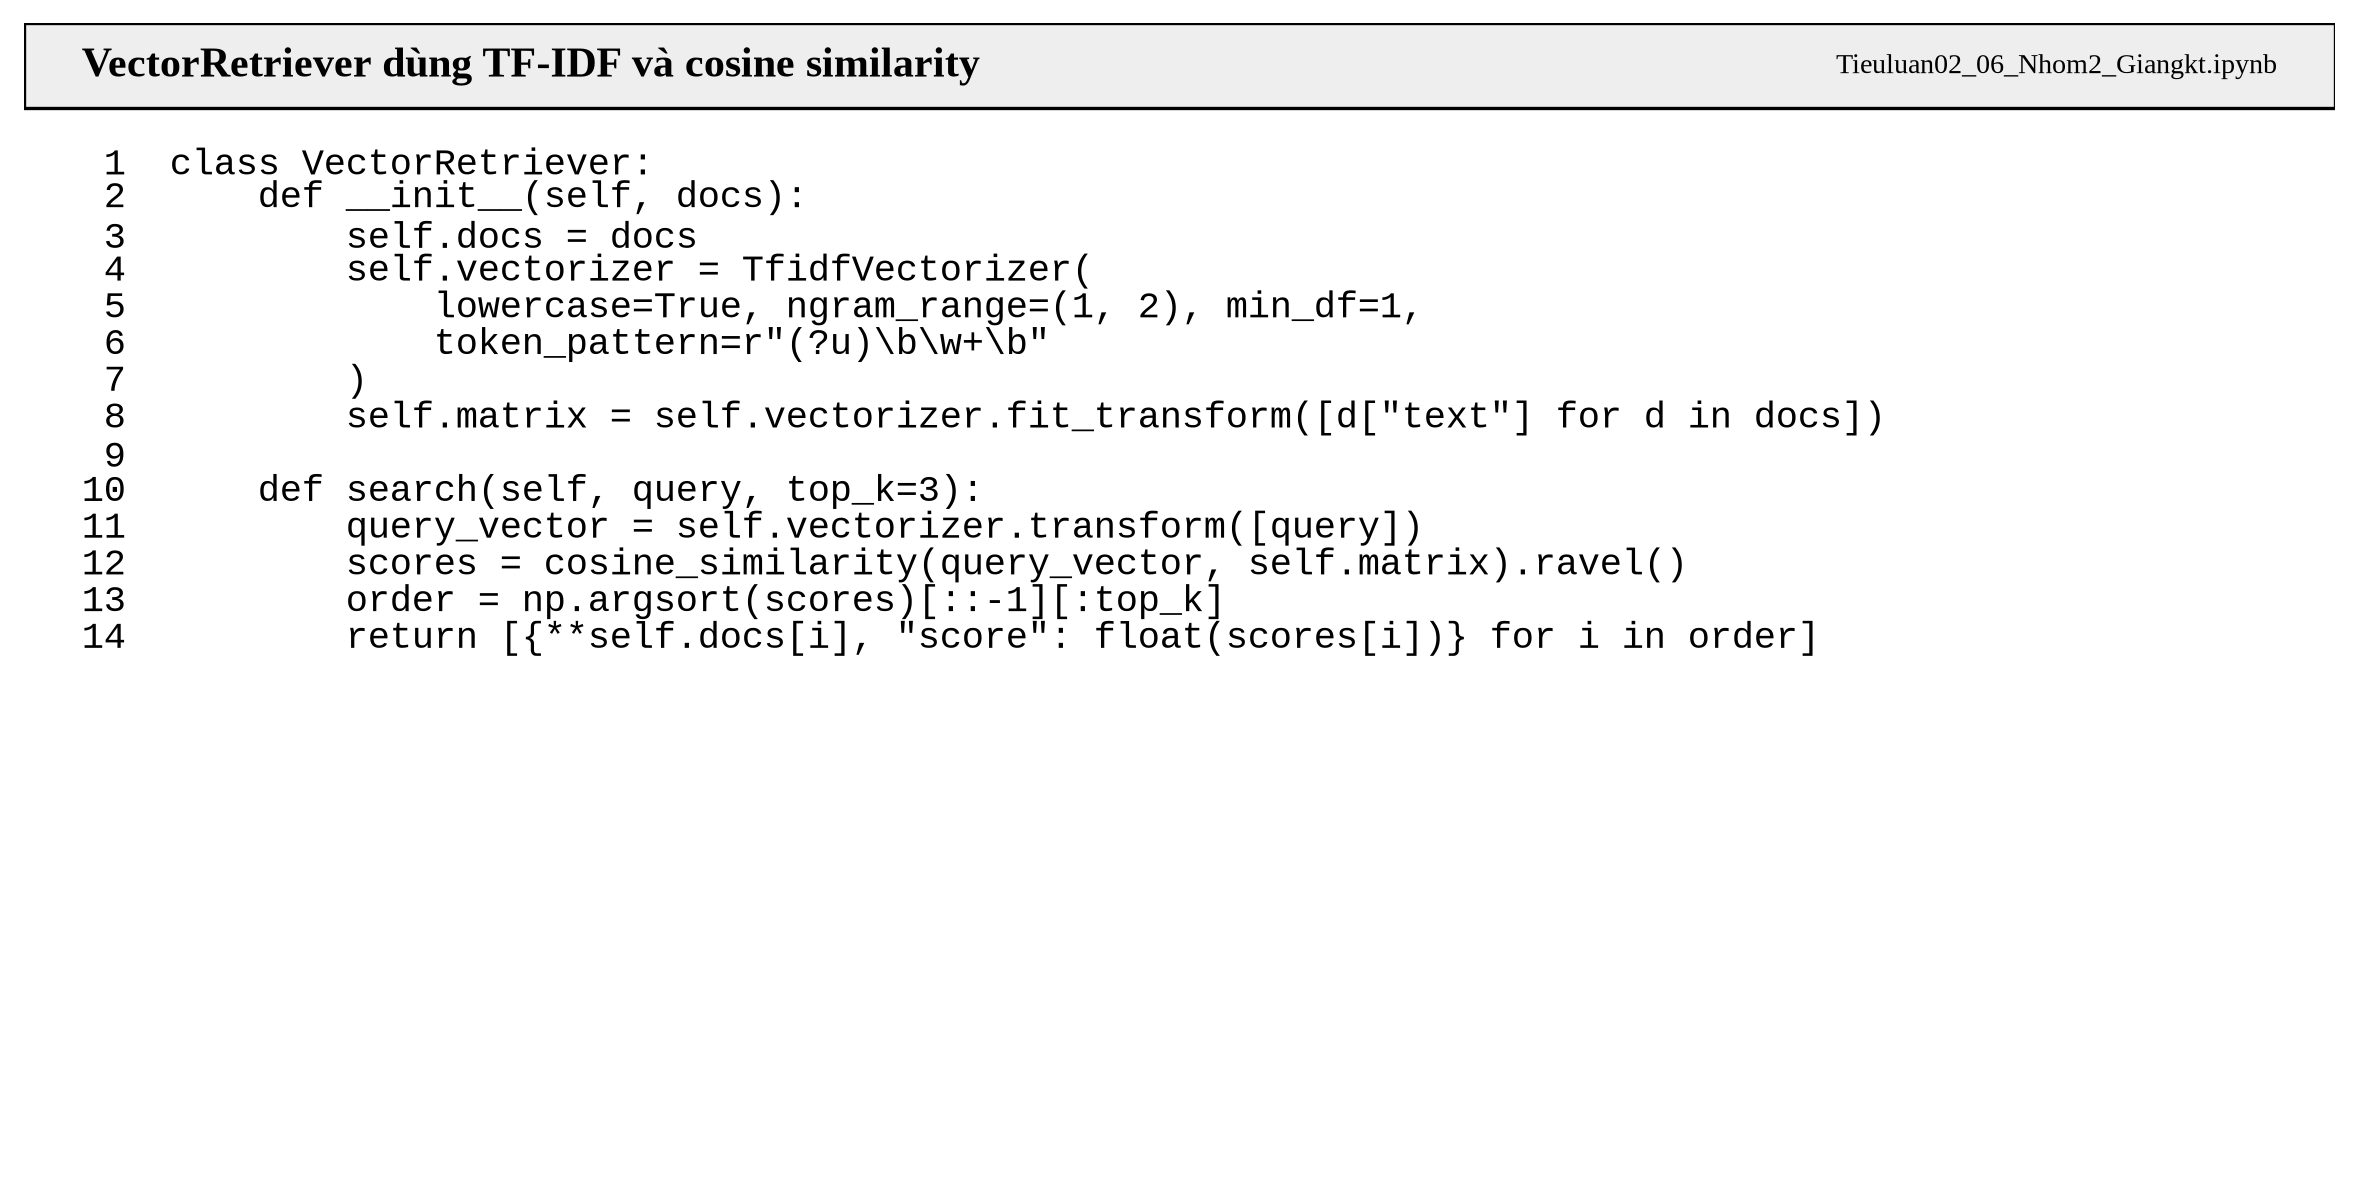
\includegraphics[width=\linewidth,height=.56\textheight,keepaspectratio]{media/media/image27.png}
\caption{Lập chỉ mục và truy xuất TF-IDF}\label{fig:legacy-5.6}
\end{figure}



\subsection{Truy xuất đồ thị và suy luận nhiều bước}\label{truy-xuux1ea5t-ux111ux1ed3-thux1ecb-vuxe0-suy-luux1eadn-nhiux1ec1u-bux1b0ux1edbc}

graph\_evidence nhận diện miền, chọn các nút cùng domain hoặc trùng từ
khóa, rồi lấy quan hệ vào và ra. Phương án này đủ cho đồ thị nhỏ. Khi đồ
thị lớn, cần entity linking, tìm kiếm theo embedding của nhãn và truy
vấn Cypher có giới hạn.

Suy luận nhiều bước được minh họa bởi chuỗi Rủi ro địa chính trị → Nhu
cầu trú ẩn → Vàng quốc tế. Vector search có thể tìm một đoạn nói về địa
chính trị nhưng không mặc nhiên biểu diễn hai quan hệ riêng. Đồ thị giúp
giữ cấu trúc của lời giải thích.

Đường đi chỉ là bằng chứng cấu trúc, không tự chứng minh nhân quả. Mọi
kết luận vẫn phụ thuộc chất lượng cạnh và nguồn đã dùng để tạo cạnh.

\begin{figure}[H]
\centering
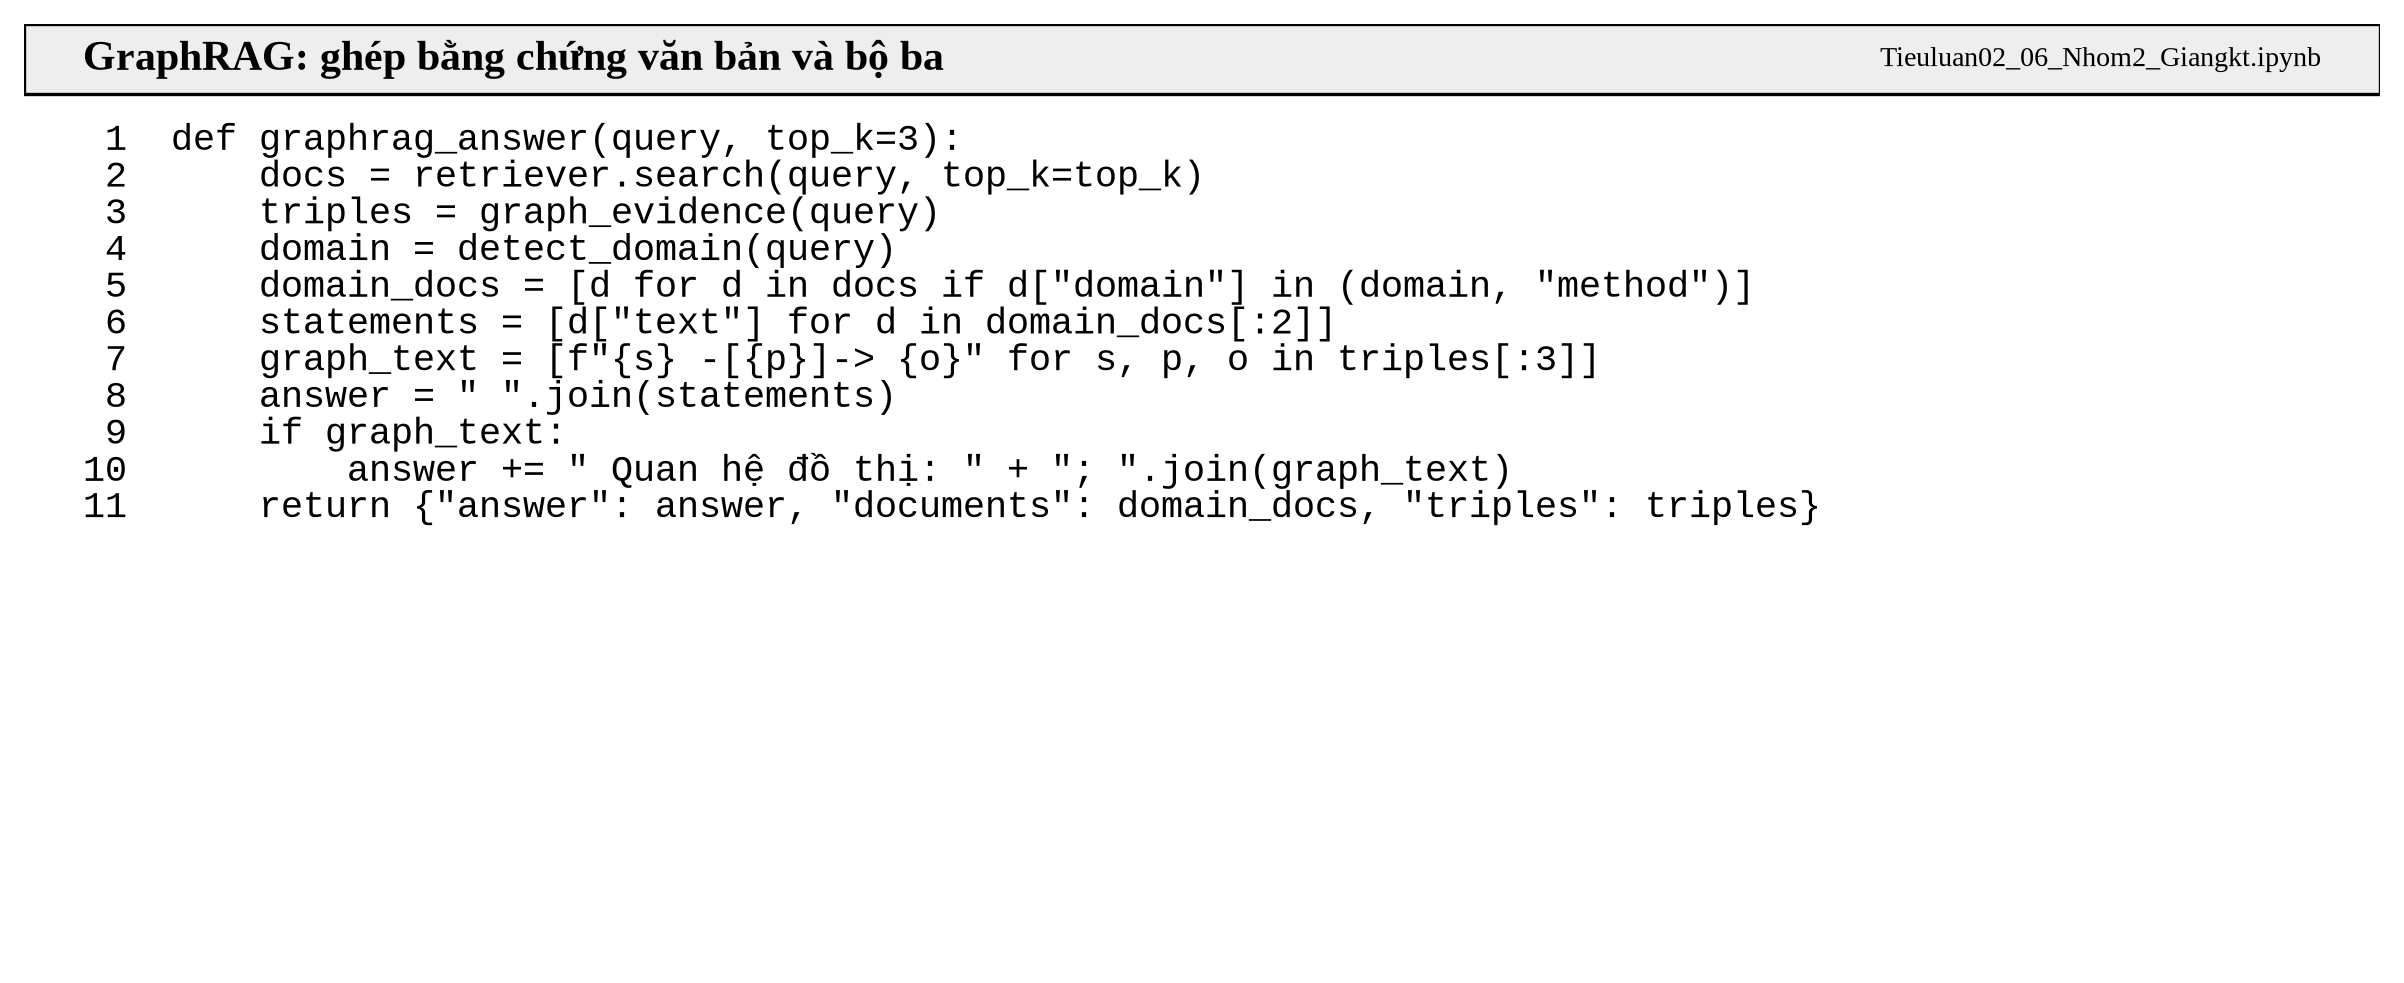
\includegraphics[width=\linewidth,height=.56\textheight,keepaspectratio]{media/media/image28.png}
\caption{Truy xuất bằng chứng đồ thị}\label{fig:legacy-5.7}
\end{figure}



\subsection{Tổng hợp câu trả lời có căn cứ}\label{tux1ed5ng-hux1ee3p-cuxe2u-trux1ea3-lux1eddi-cuxf3-cux103n-cux1ee9}

Bộ sinh trong bài là deterministic synthesizer. Nó chọn hai tài liệu phù
hợp, nối tối đa ba quan hệ đồ thị và thêm cảnh báo theo miền. Kết quả ít
tự nhiên hơn LLM nhưng có lợi thế là chạy offline và không tự thêm sự
kiện ngoài bằng chứng.

Có thể thay bộ sinh bằng một LLM cục bộ hoặc dịch vụ API. Khi đó prompt
phải tách rõ QUESTION, TEXT EVIDENCE, GRAPH EVIDENCE và yêu cầu từ chối
nếu bằng chứng thiếu. Đầu ra nên ở dạng JSON để kiểm tra citation\_id.

Thiết kế production cần chống prompt injection từ tài liệu, lọc dữ liệu
nhạy cảm, theo dõi phiên bản chỉ mục và ghi log các nguồn đã đưa cho mô
hình.

\subsection{Đánh giá RAG và GraphRAG}\label{ux111uxe1nh-giuxe1-RAG-vuxe0-GraphRAG}

Bộ kiểm thử gồm sáu câu hỏi, hai câu cho mỗi miền. vector\_precision@3
đo tỷ lệ tài liệu thuộc đúng miền trong ba kết quả đầu. graph\_evidence
ghi nhận hệ thống có tìm được cạnh liên quan hay không. Điểm tổng hợp
cộng một phần thưởng nhỏ khi cả hai kênh đều có bằng chứng.

Ở lần chạy này, precision@3 trung bình là 0.500; tỷ lệ câu hỏi có bằng
chứng đồ thị là 1.000; điểm bằng chứng lai là 0.750.

Đây là smoke test, chưa phải benchmark khoa học. Một đánh giá đầy đủ cần
nhiều câu hỏi do người độc lập soạn, đáp án chuẩn, chấm faithfulness,
answer relevance, citation correctness, độ trễ và chi phí.

\begin{figure}[H]
\centering
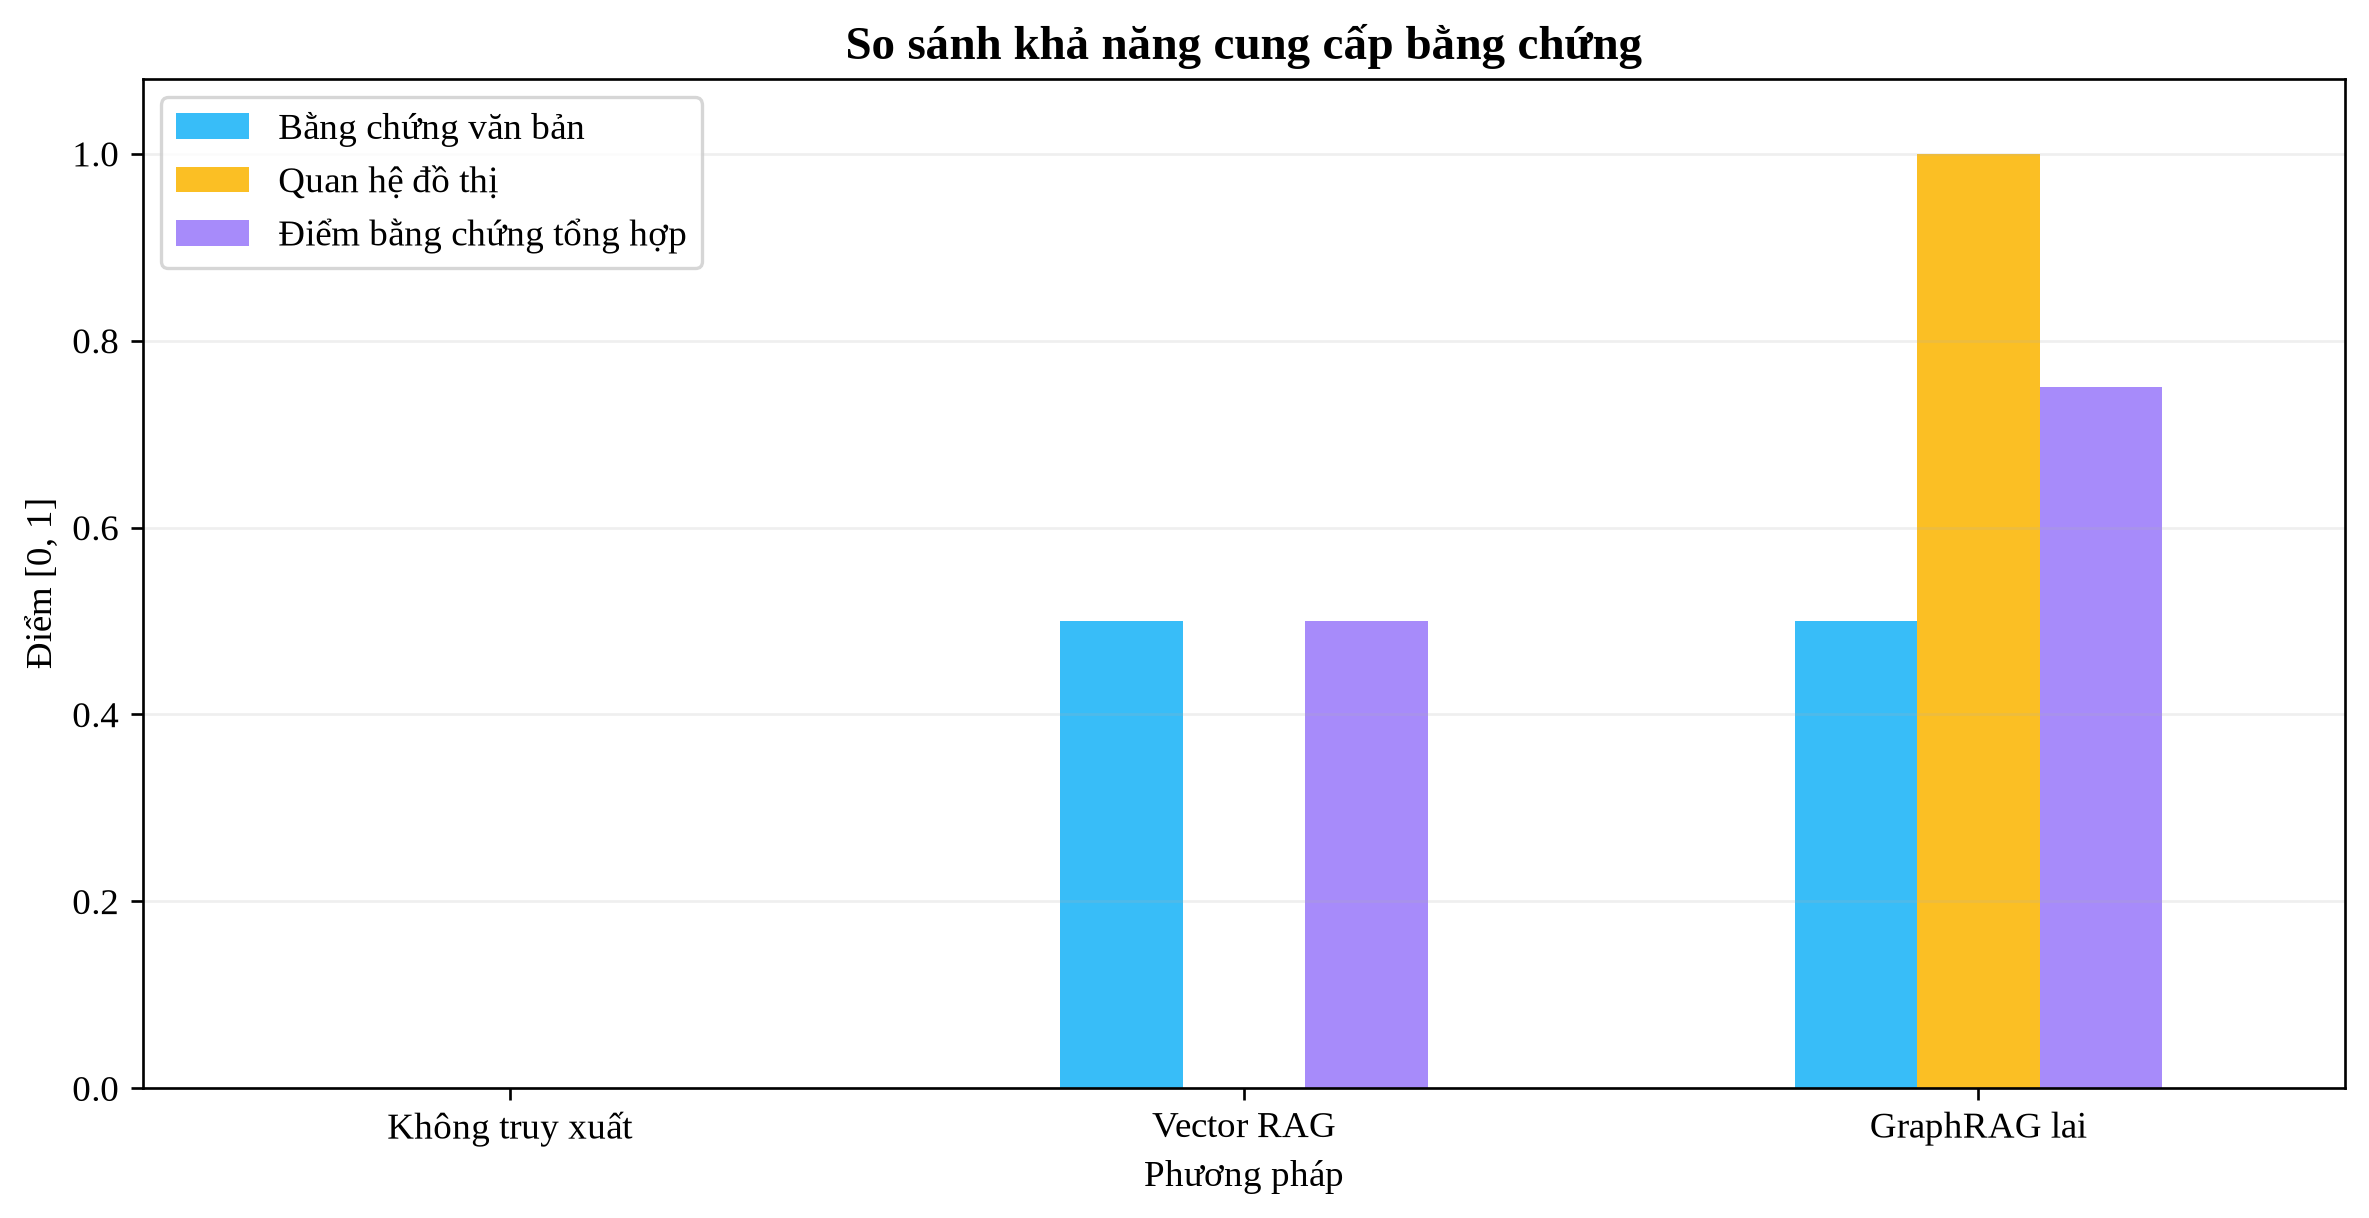
\includegraphics[width=\linewidth,height=.56\textheight,keepaspectratio]{media/media/image29.png}
\caption{Đánh giá smoke test RAG và GraphRAG}\label{fig:legacy-5.8}
\end{figure}



\section{KB và RAG cho bệnh tiểu đường}\label{KB-vuxe0-RAG-cho-bux1ec7nh-tiux1ec3u-ux111ux1b0ux1eddng}

Dữ liệu diabetes gồm 442 người đã mắc bệnh, 10 thuộc tính nền và điểm
tiến triển sau một năm. Đầu ra là hồi quy nghiên cứu, không phải xác
suất mắc tiểu đường.

Dữ liệu được chia thành 282 mẫu train, 71 mẫu hiệu chỉnh khoảng dự báo
và 89 mẫu test. K-fold 5 phần chỉ chạy trên train; so sánh Median
baseline, Linear, Ridge, ElasticNet, Huber, SVR RBF, Random Forest và
Gradient Boosting. Thêm mô hình phi tuyến không đồng nghĩa chắc chắn tốt
hơn; quyết định vẫn dựa trên CV MAE.

Mô hình được chọn theo CV: Ridge; CV MAE 44.44; test MAE 42.94; R2
0.452. MAE của dự báo trung vị là 62.28. Khoảng dự báo mục tiêu 90\% có
độ bao phủ test 86.5\%.

\begin{figure}[H]
\centering
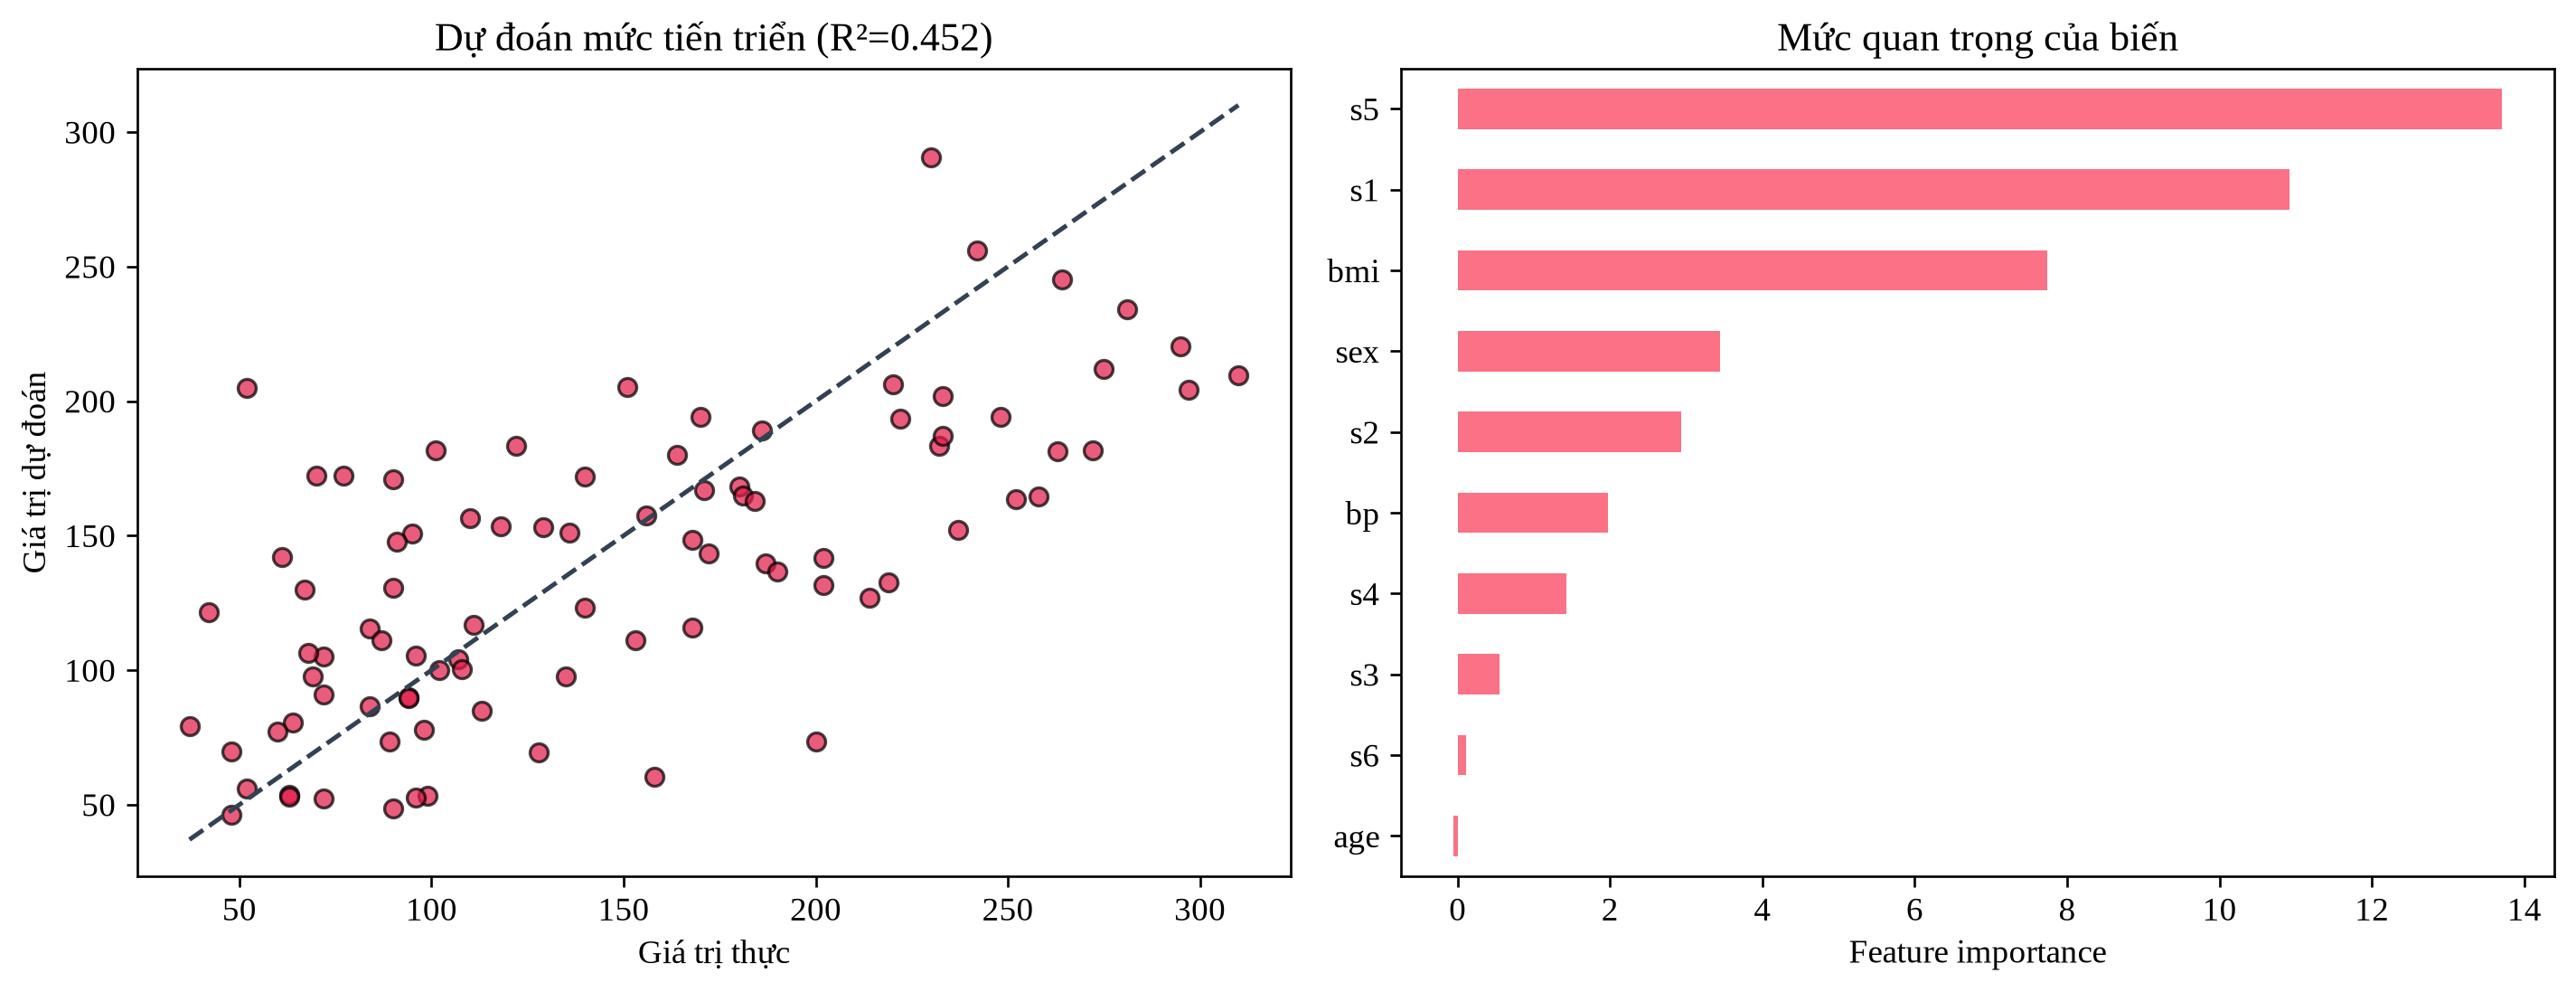
\includegraphics[width=\linewidth,height=.56\textheight,keepaspectratio]{media/media/image30.png}
\caption{Mô hình hồi quy tiến triển tiểu đường}\label{fig:legacy-5.9}
\end{figure}



\subsection{Ontology và xử lý dữ liệu y tế}\label{ontology-vuxe0-xux1eed-luxfd-dux1eef-liux1ec7u-y-tux1ebf}

Ontology tối giản gồm Condition, Biomarker, RiskFactor, Lifestyle,
Monitoring và Professional. Các quan hệ như LIÊN\_QUAN\_ĐẾN hoặc
HỖ\_TRỢ\_QUẢN\_LÝ được chọn để tránh biến một tương quan thành chỉ định
điều trị.

Dữ liệu không có tên bệnh nhân hay định danh cá nhân. Trong tình huống
thực, hồ sơ y tế cần mã hóa, phân quyền theo vai trò, nhật ký truy cập
và quy trình chấp thuận. Không nên đưa thông tin nhận dạng vào dịch vụ
embedding công cộng khi chưa có cơ sở pháp lý.

Mô hình Ridge được chọn theo MAE trung bình của 5 fold. Permutation
importance được tính trên tập test để cùng một cách giải thích áp dụng
được cho cả mô hình tuyến tính và mô hình cây.

\begin{figure}[H]
\centering
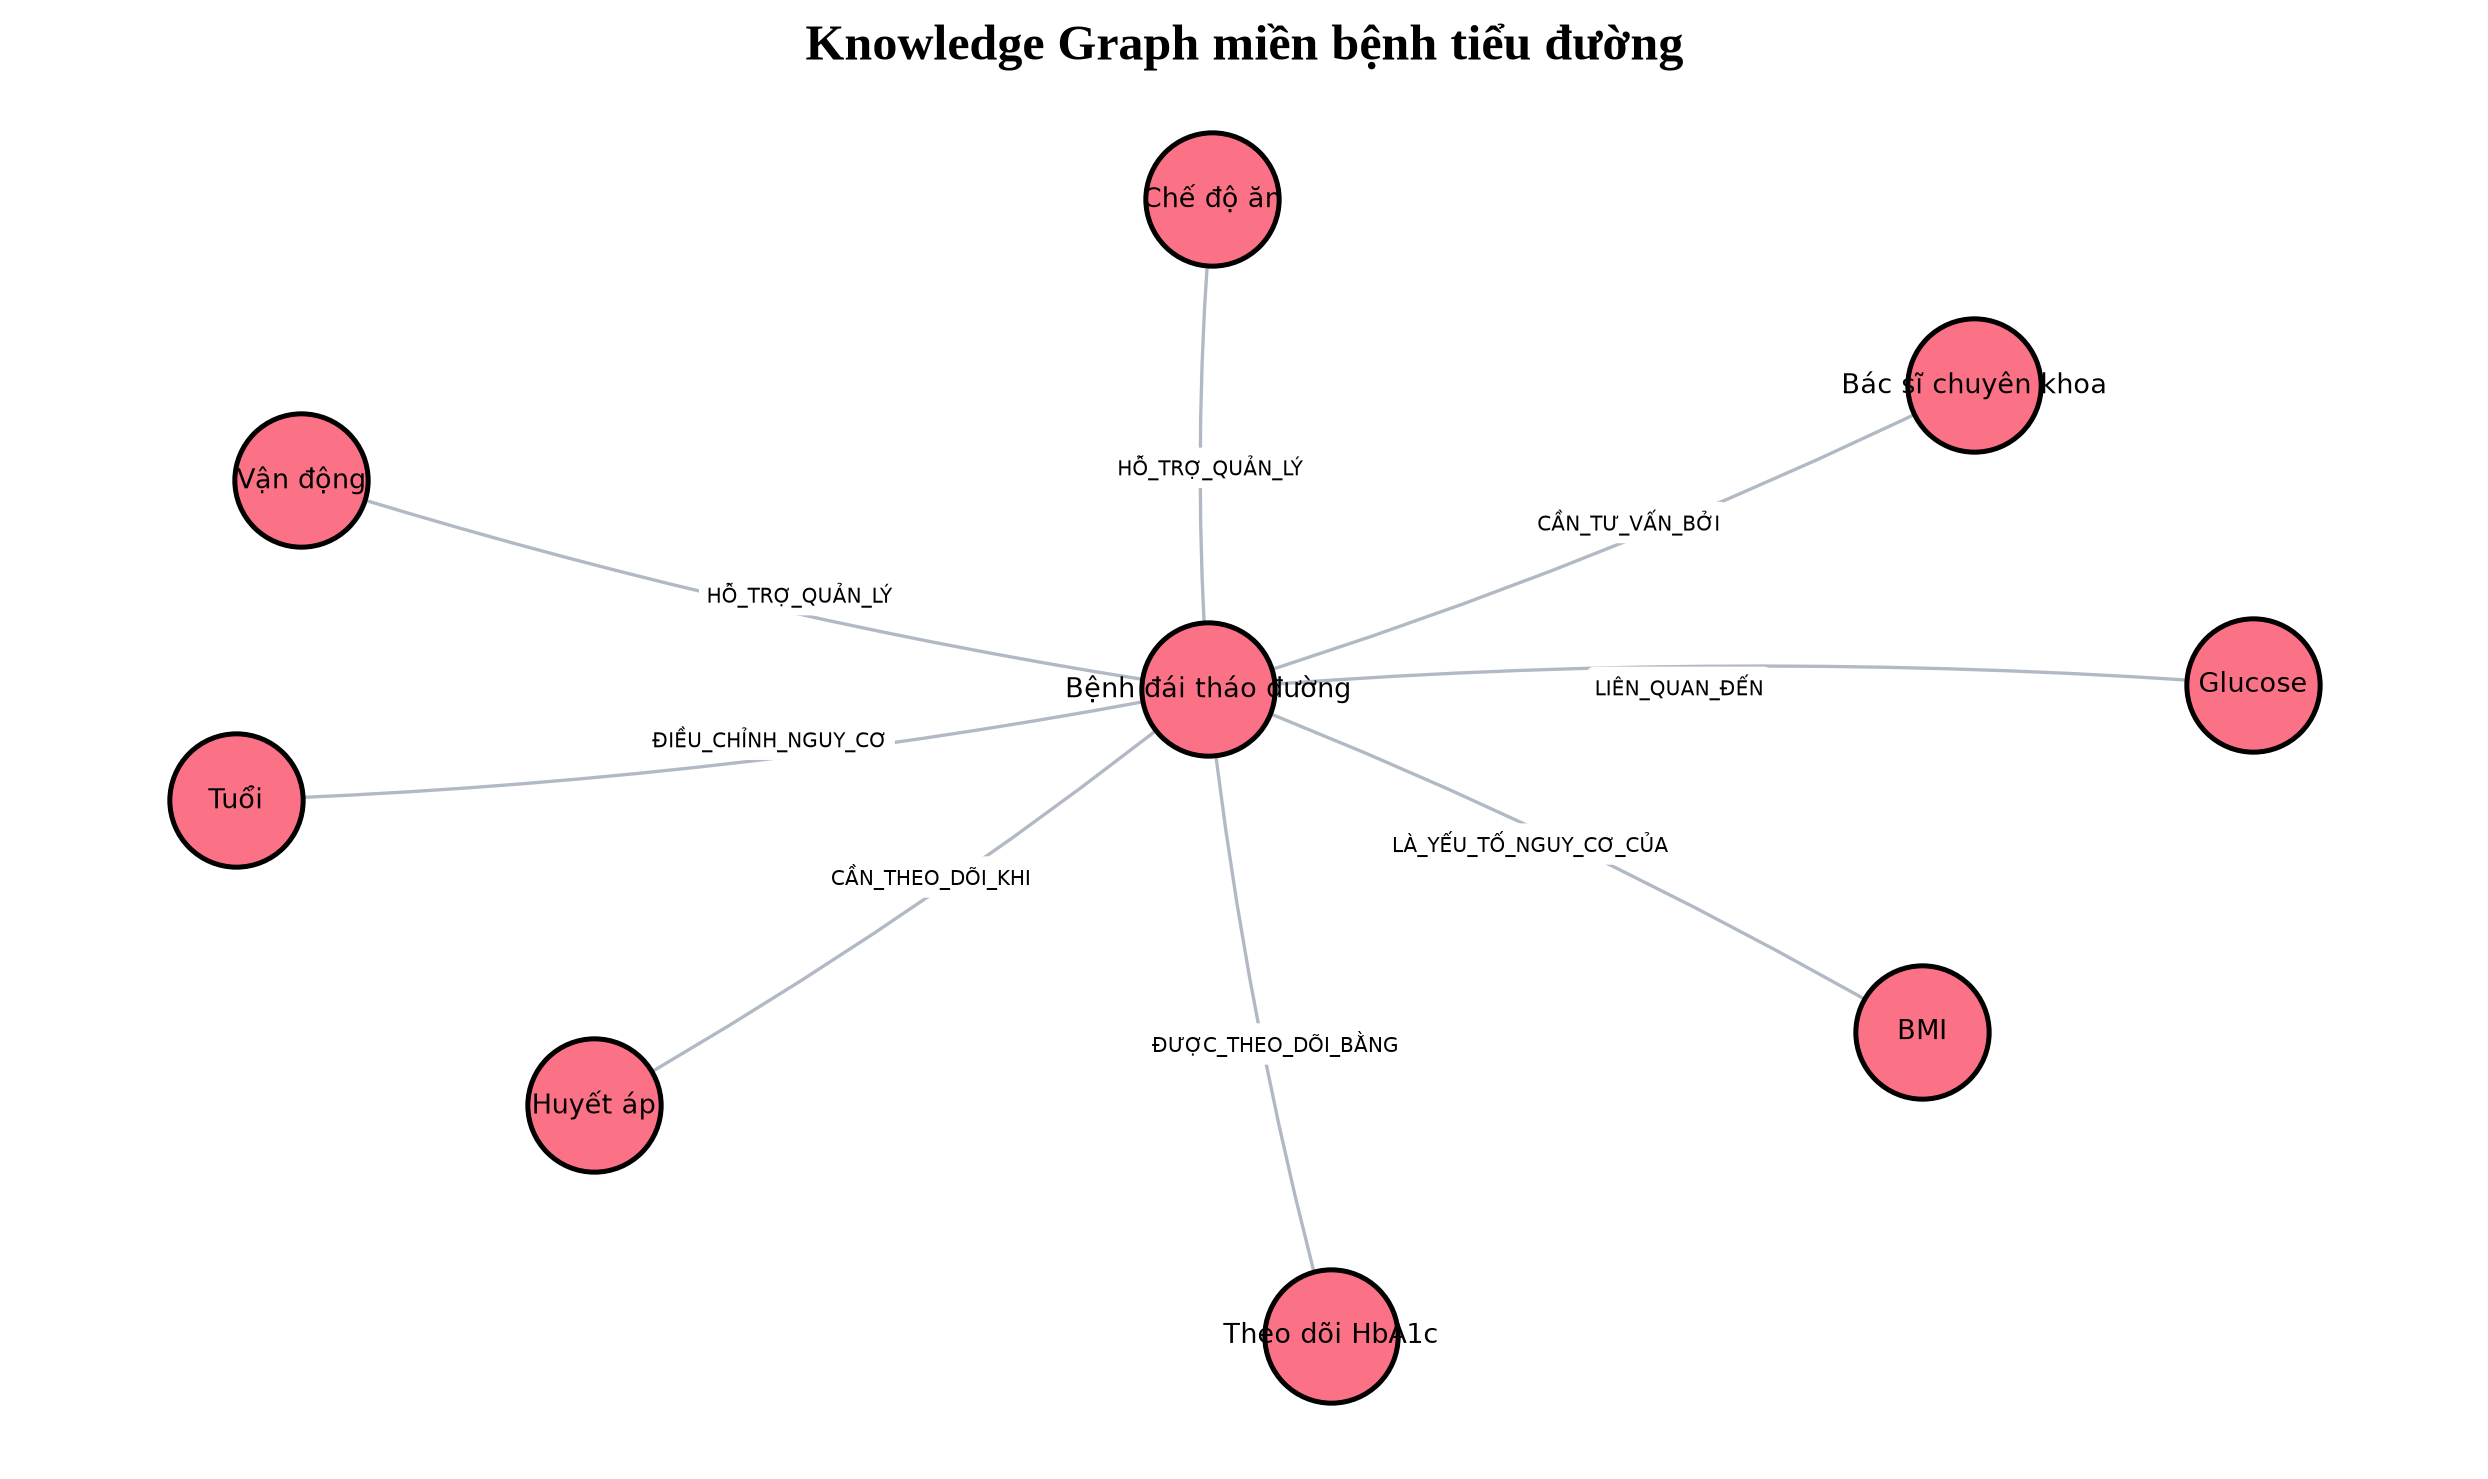
\includegraphics[width=\linewidth,height=.56\textheight,keepaspectratio]{media/media/image31.png}
\caption{Đồ thị tri thức y tế}\label{fig:legacy-5.10}
\end{figure}



\subsection{Thực nghiệm hỏi đáp y tế}\label{thux1ef1c-nghiux1ec7m-hux1ecfi-ux111uxe1p-y-tux1ebf}

Câu hỏi mẫu hỏi các yếu tố liên quan đến quản lý bệnh tiểu đường. Vector
retriever tìm mô tả theo dõi đường huyết, HbA1c, huyết áp, cân nặng, ăn
uống và vận động. Đồ thị bổ sung các cạnh nối bệnh với theo dõi và
chuyên gia.

Câu trả lời sinh ra trong lần chạy: Theo dõi đường huyết, HbA1c, huyết
áp, cân nặng, chế độ ăn và vận động là các thành phần thường gặp trong
quản lý bệnh đái tháo đường; quyết định điều trị cần bác sĩ. Bộ dữ liệu
diabetes của scikit-learn có 442 quan sát, 10 biến nền ở thang đo gốc và
biến đích phản ánh mức tiến triển bệnh sau một năm. Quan hệ đồ thị liên
quan: Bệnh đái tháo đường -{[}ĐƯỢC\_THEO\_DÕI\_BẰNG{]}→ Theo dõi HbA1c;
Bệnh đái tháo đường -{[}CẦN\_TƯ\_VẤN\_BỞI{]}→ Bác sĩ chuyên khoa;
Glucose -{[}LIÊN\_QUAN\_ĐẾN{]}→ Bệnh đái tháo đường. Kết quả chỉ có giá
trị minh họa; cần tham khảo nhân viên y tế cho quyết định cá nhân.

Biểu đồ đối chiếu giá trị thực - dự đoán và feature importance cho thấy
mức độ phù hợp cũng như biến nào được mô hình sử dụng nhiều nhất.

\begin{figure}[H]
\centering
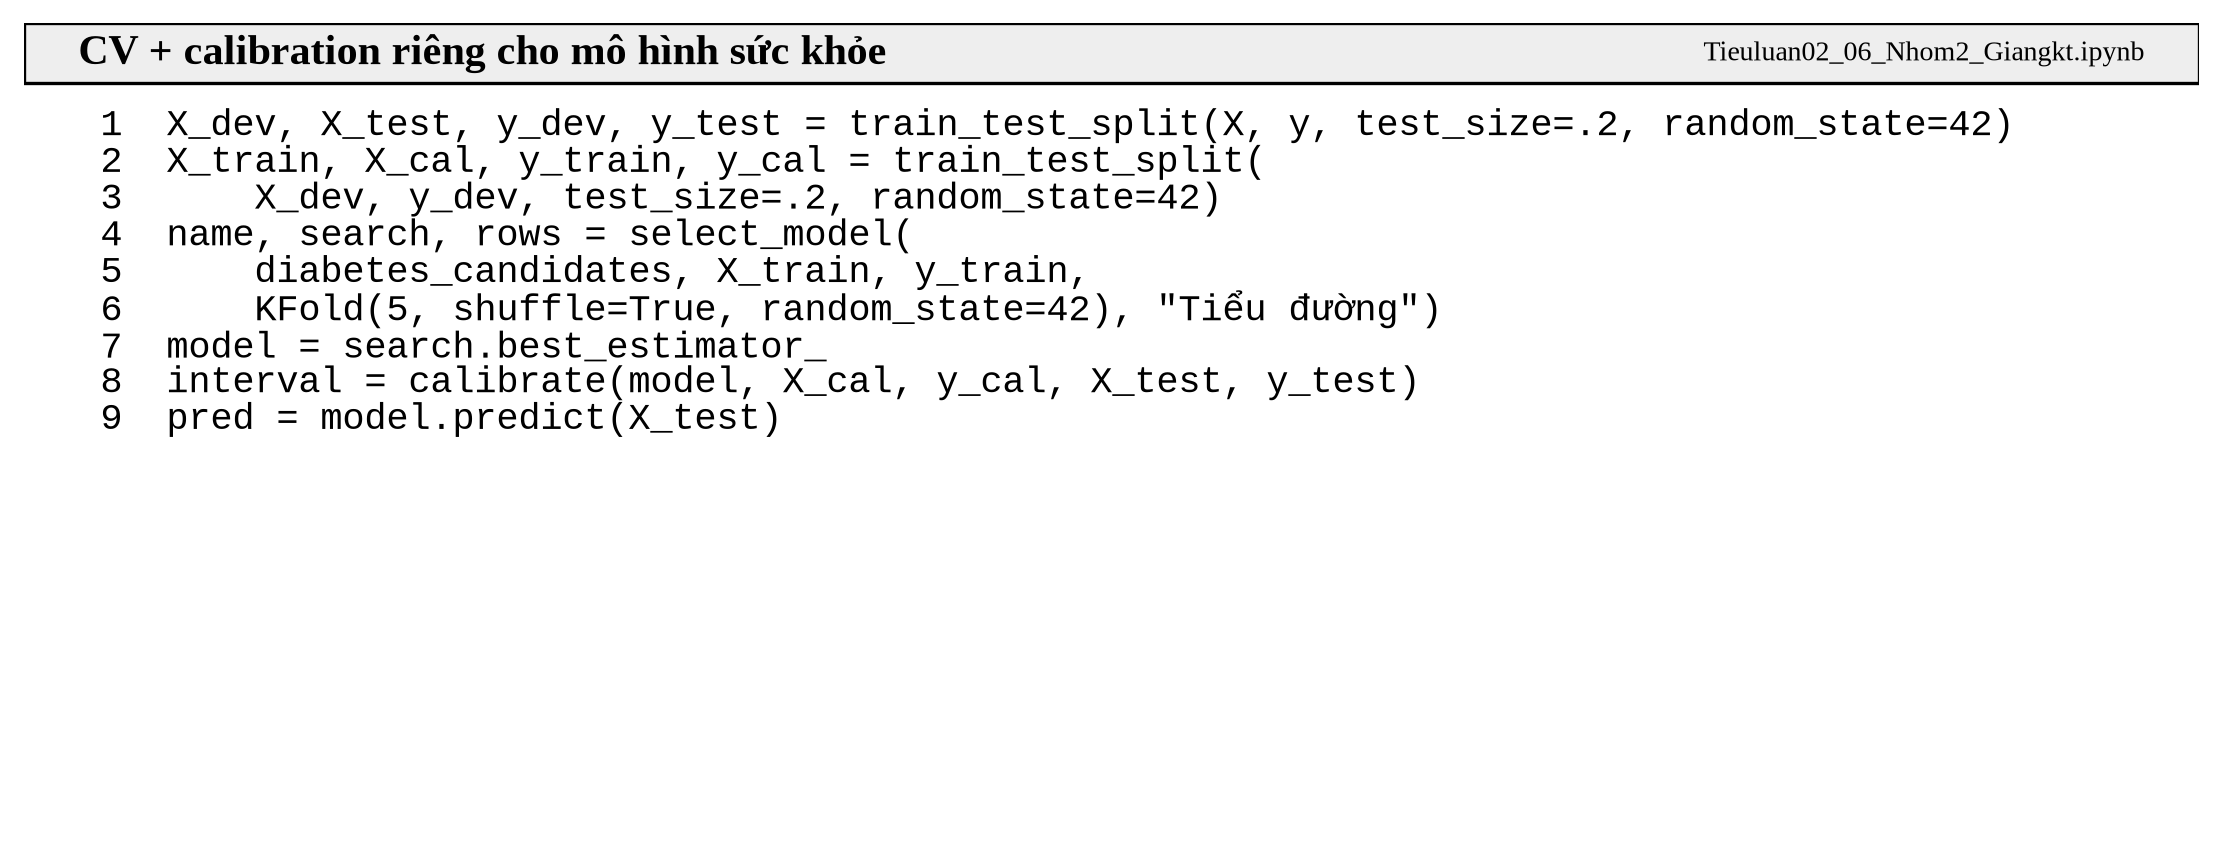
\includegraphics[width=\linewidth,height=.56\textheight,keepaspectratio]{media/media/image32.png}
\caption{Huấn luyện và đánh giá mô hình y tế}\label{fig:legacy-5.11}
\end{figure}



\subsection{Giới hạn và hướng mở rộng y tế}\label{giux1edbi-hux1ea1n-vuxe0-hux1b0ux1edbng-mux1edf-rux1ed9ng-y-tux1ebf}

Bộ dữ liệu nhỏ, không đại diện cho dân số Việt Nam và không chứa bối
cảnh điều trị. Chỉ số đích mang ý nghĩa nghiên cứu, khác với chẩn đoán
đái tháo đường trong thực hành. Vì vậy không thể suy rộng độ chính xác
mô hình thành hiệu quả lâm sàng.

Hướng mở rộng là dùng dữ liệu đã khử định danh, xác định rõ biến kết
cục, đánh giá theo nhóm tuổi/giới và mời chuyên gia lâm sàng kiểm tra
ontology. Ngoài độ chính xác, cần đo calibration, fairness và khả năng
giải thích.

Với RAG y tế, mọi đoạn văn cần version và ngày hiệu lực. Hướng dẫn cũ
phải được thu hồi khỏi chỉ mục thay vì chỉ thêm tài liệu mới.

\section{KB và RAG cho chứng khoán}\label{KB-vuxe0-RAG-cho-chux1ee9ng-khouxe1n}

Dữ liệu FPT.VN được lấy từ Yahoo Finance chart API - FPT.VN. Khoảng thời
gian 15/10/2021 - 14/10/2026 có 1304 quan sát. Giá đóng cửa gần nhất là
57,100 VND.

Lợi suất toàn kỳ là 15.91\%, biến động năm hóa 27.63\%, RSI14 8.2. Mỗi
con số được gắn ngày chạy và nguồn dữ liệu.

Knowledge Graph nối FPT.VN với giá gần nhất, MA20, MA60, RSI, thanh
khoản, kết quả kinh doanh và tâm lý thị trường. Các quan hệ mô tả vai
trò chỉ báo, không tự động tạo khuyến nghị mua bán.

\begin{figure}[H]
\centering
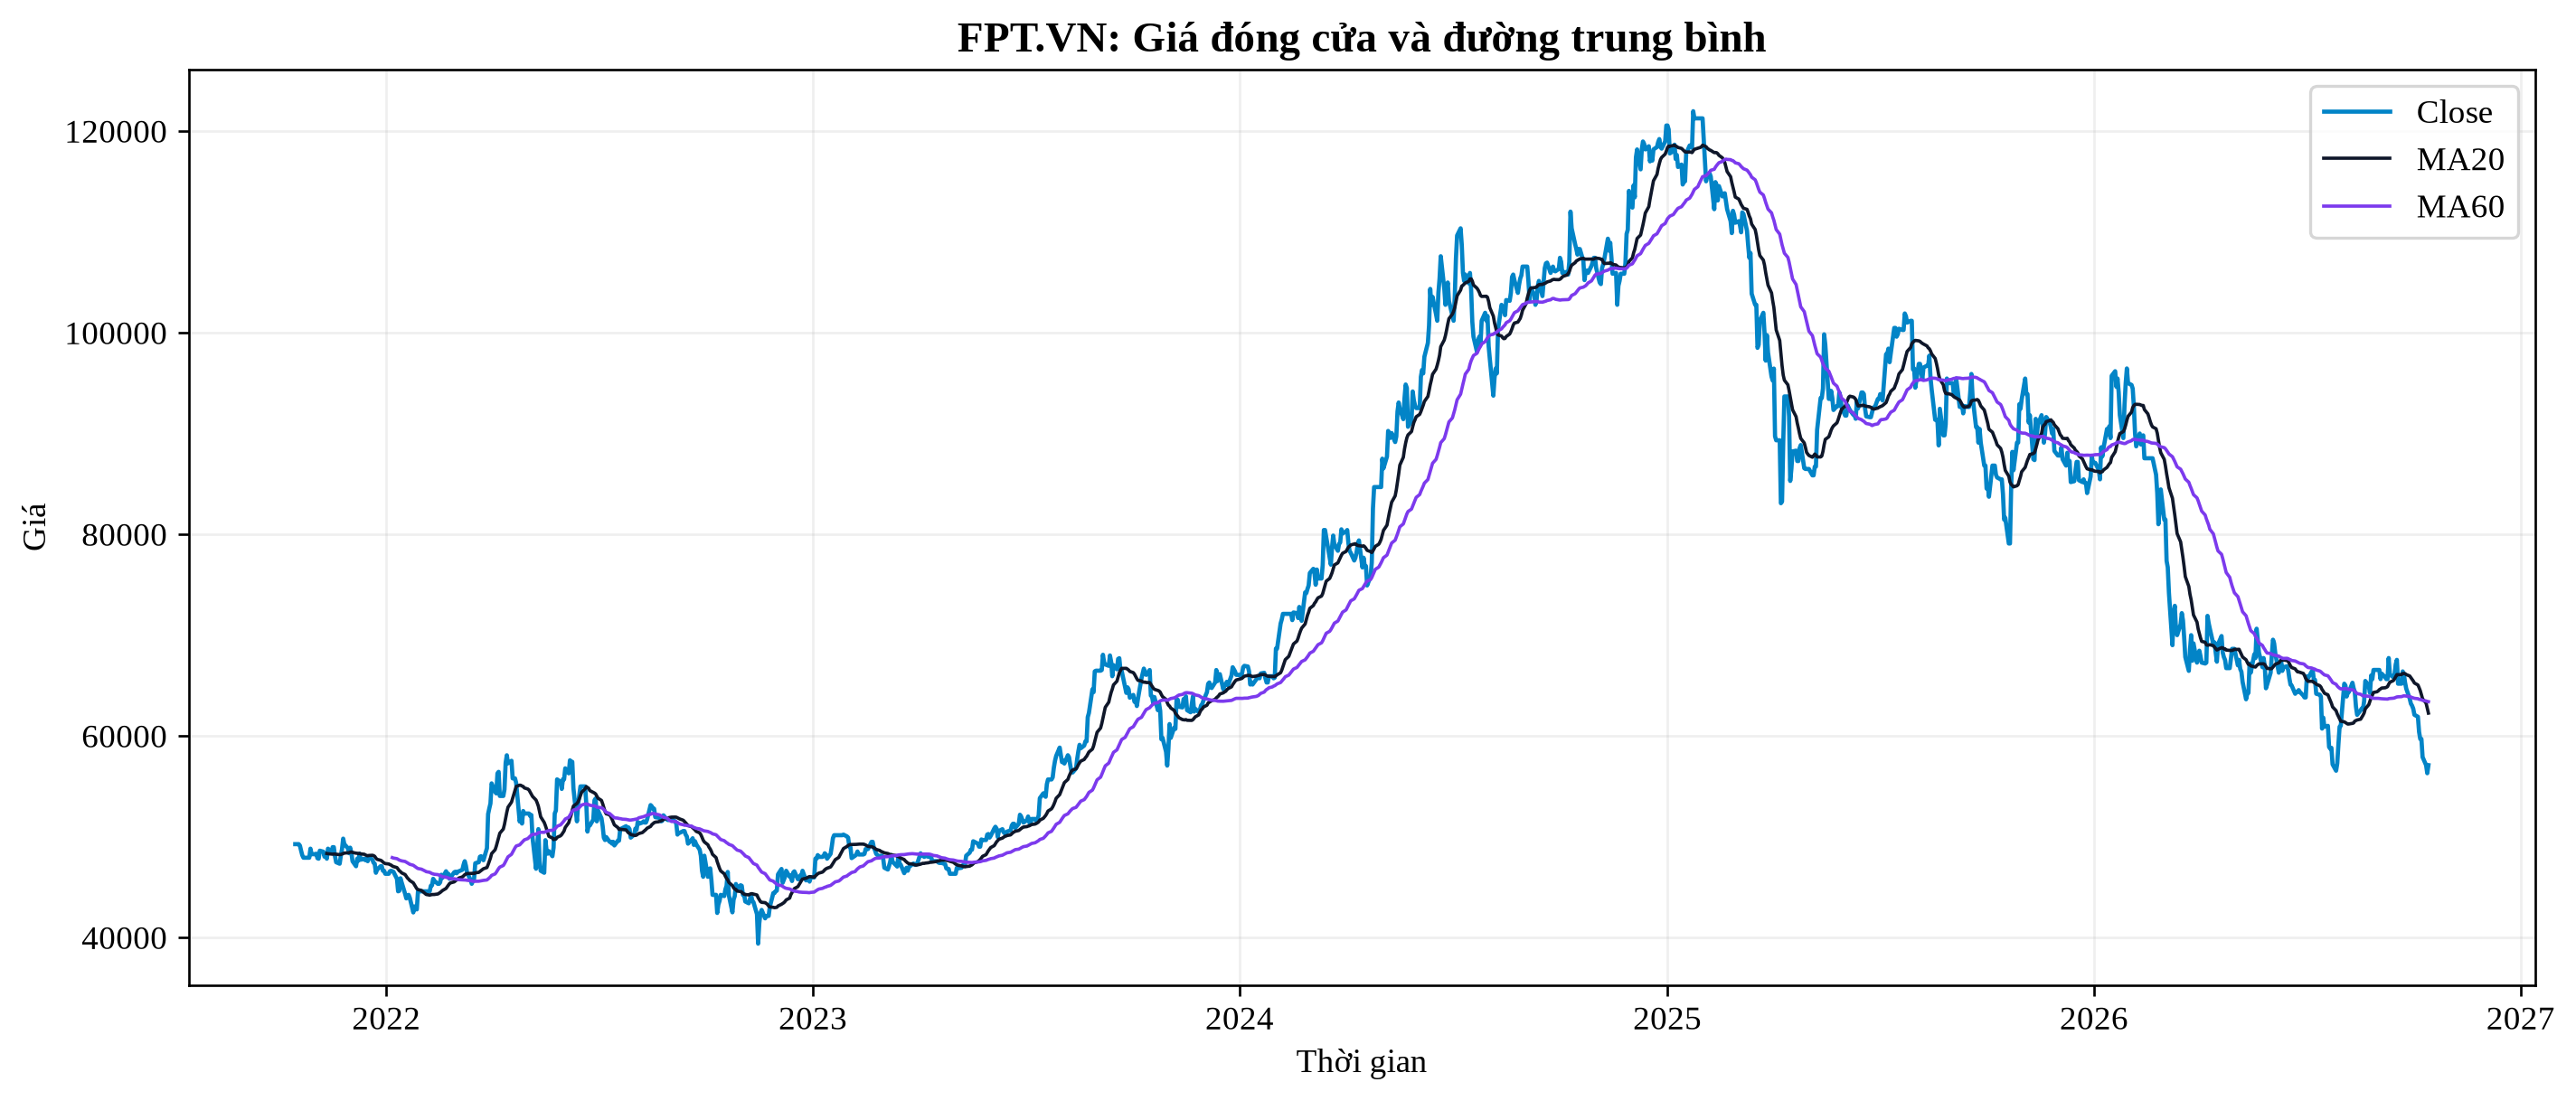
\includegraphics[width=\linewidth,height=.56\textheight,keepaspectratio]{media/media/image33.png}
\caption{Chuỗi giá và chỉ báo FPT}\label{fig:legacy-5.12}
\end{figure}



\subsection{Dữ liệu và tiền xử lý FPT}\label{dux1eef-liux1ec7u-vuxe0-tiux1ec1n-xux1eed-luxfd-fpt}

Chuỗi OHLCV được sắp xếp tăng dần theo ngày; dòng thiếu Close bị loại.
Return\_1D, MA20, MA60, volatility20 và RSI14 được tính từ dữ liệu lịch
sử. Đặc trưng bổ sung gồm thay đổi khối lượng, biên độ High-Low, chênh
lệch Open-Close và các độ trễ một phiên.

Tại điểm cuối, MA20 = 62,260, MA60 = 63,396. Bộ học có 988 mẫu train và
85 mẫu test theo thứ tự thời gian.

Biến đích là giá Close của phiên kế tiếp. Việc dịch target một bước rồi
drop dòng cuối giúp đặc trưng tại ngày t không chứa giá của ngày t+1.

\begin{figure}[H]
\centering
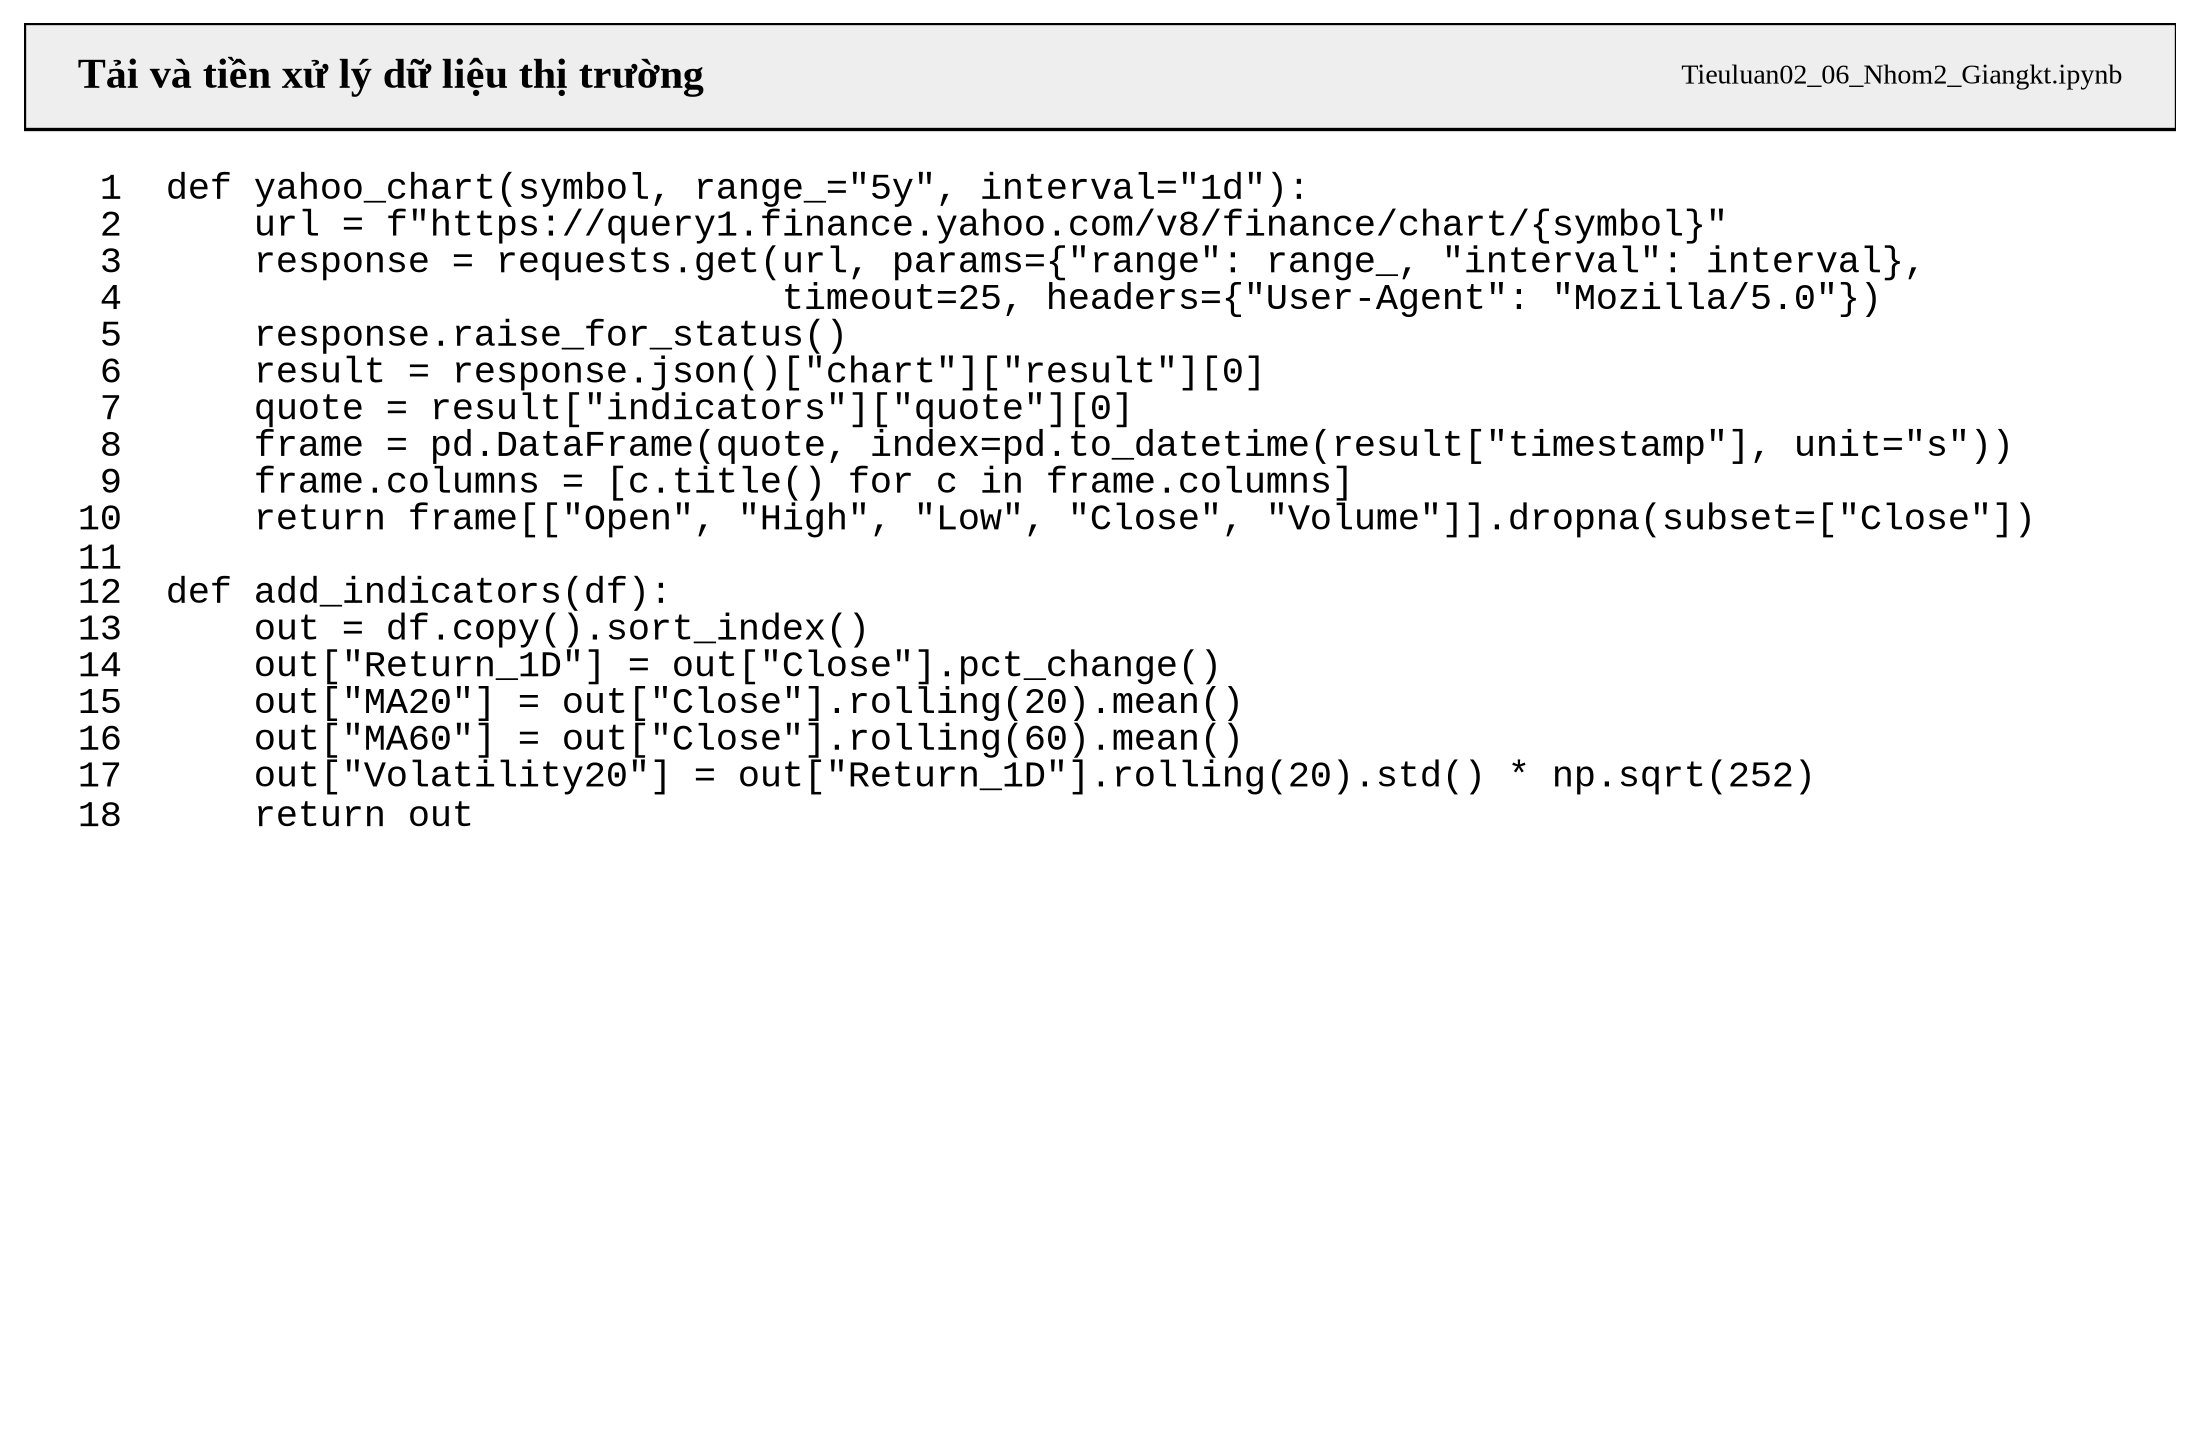
\includegraphics[width=\linewidth,height=.56\textheight,keepaspectratio]{media/media/image34.png}
\caption{Pipeline xử lý dữ liệu thị trường}\label{fig:legacy-5.13}
\end{figure}



\subsection{Huấn luyện và đánh giá mô hình FPT}\label{huux1ea5n-luyux1ec7n-vuxe0-ux111uxe1nh-giuxe1-muxf4-huxecnh-fpt}

Lịch sử tải được mở rộng từ 2 năm lên 5 năm. Chín họ cấu hình gồm
Persistence, Ridge giá, Median lợi suất, Ridge lợi suất, Huber, SVR RBF,
Random Forest và hai dạng Gradient Boosting. Tuning độ co lợi suất, cửa
sổ học gần nhất và siêu tham số trên TimeSeriesSplit 5 phần, mỗi phần
xác nhận 63 phiên, gap=1. Tập test giữ nguyên mốc của bản 2.0.

Chia theo thời gian: 988 train, 67 hiệu chỉnh, 85 test; bỏ một quan sát
tại mỗi ranh giới. Mô hình Persistence đạt MAE 728.13, R2 0.871;
baseline MAE 728.13. Cải thiện trên test 0.00\%.

Test lịch sử từ 2026-06-04 đến 2026-10-13; MAE bản trước 728.13 VND. Bao
phủ khoảng dự báo lịch sử: 97.6\%. Kết quả hiện tại chưa cho thấy mô
hình học máy thắng Persistence. Dữ liệu chuỗi thời gian không thỏa giả
định trao đổi như mẫu độc lập nên mức 90\% chỉ là mục tiêu, không phải
bảo đảm cho tương lai.

\begin{figure}[H]
\centering
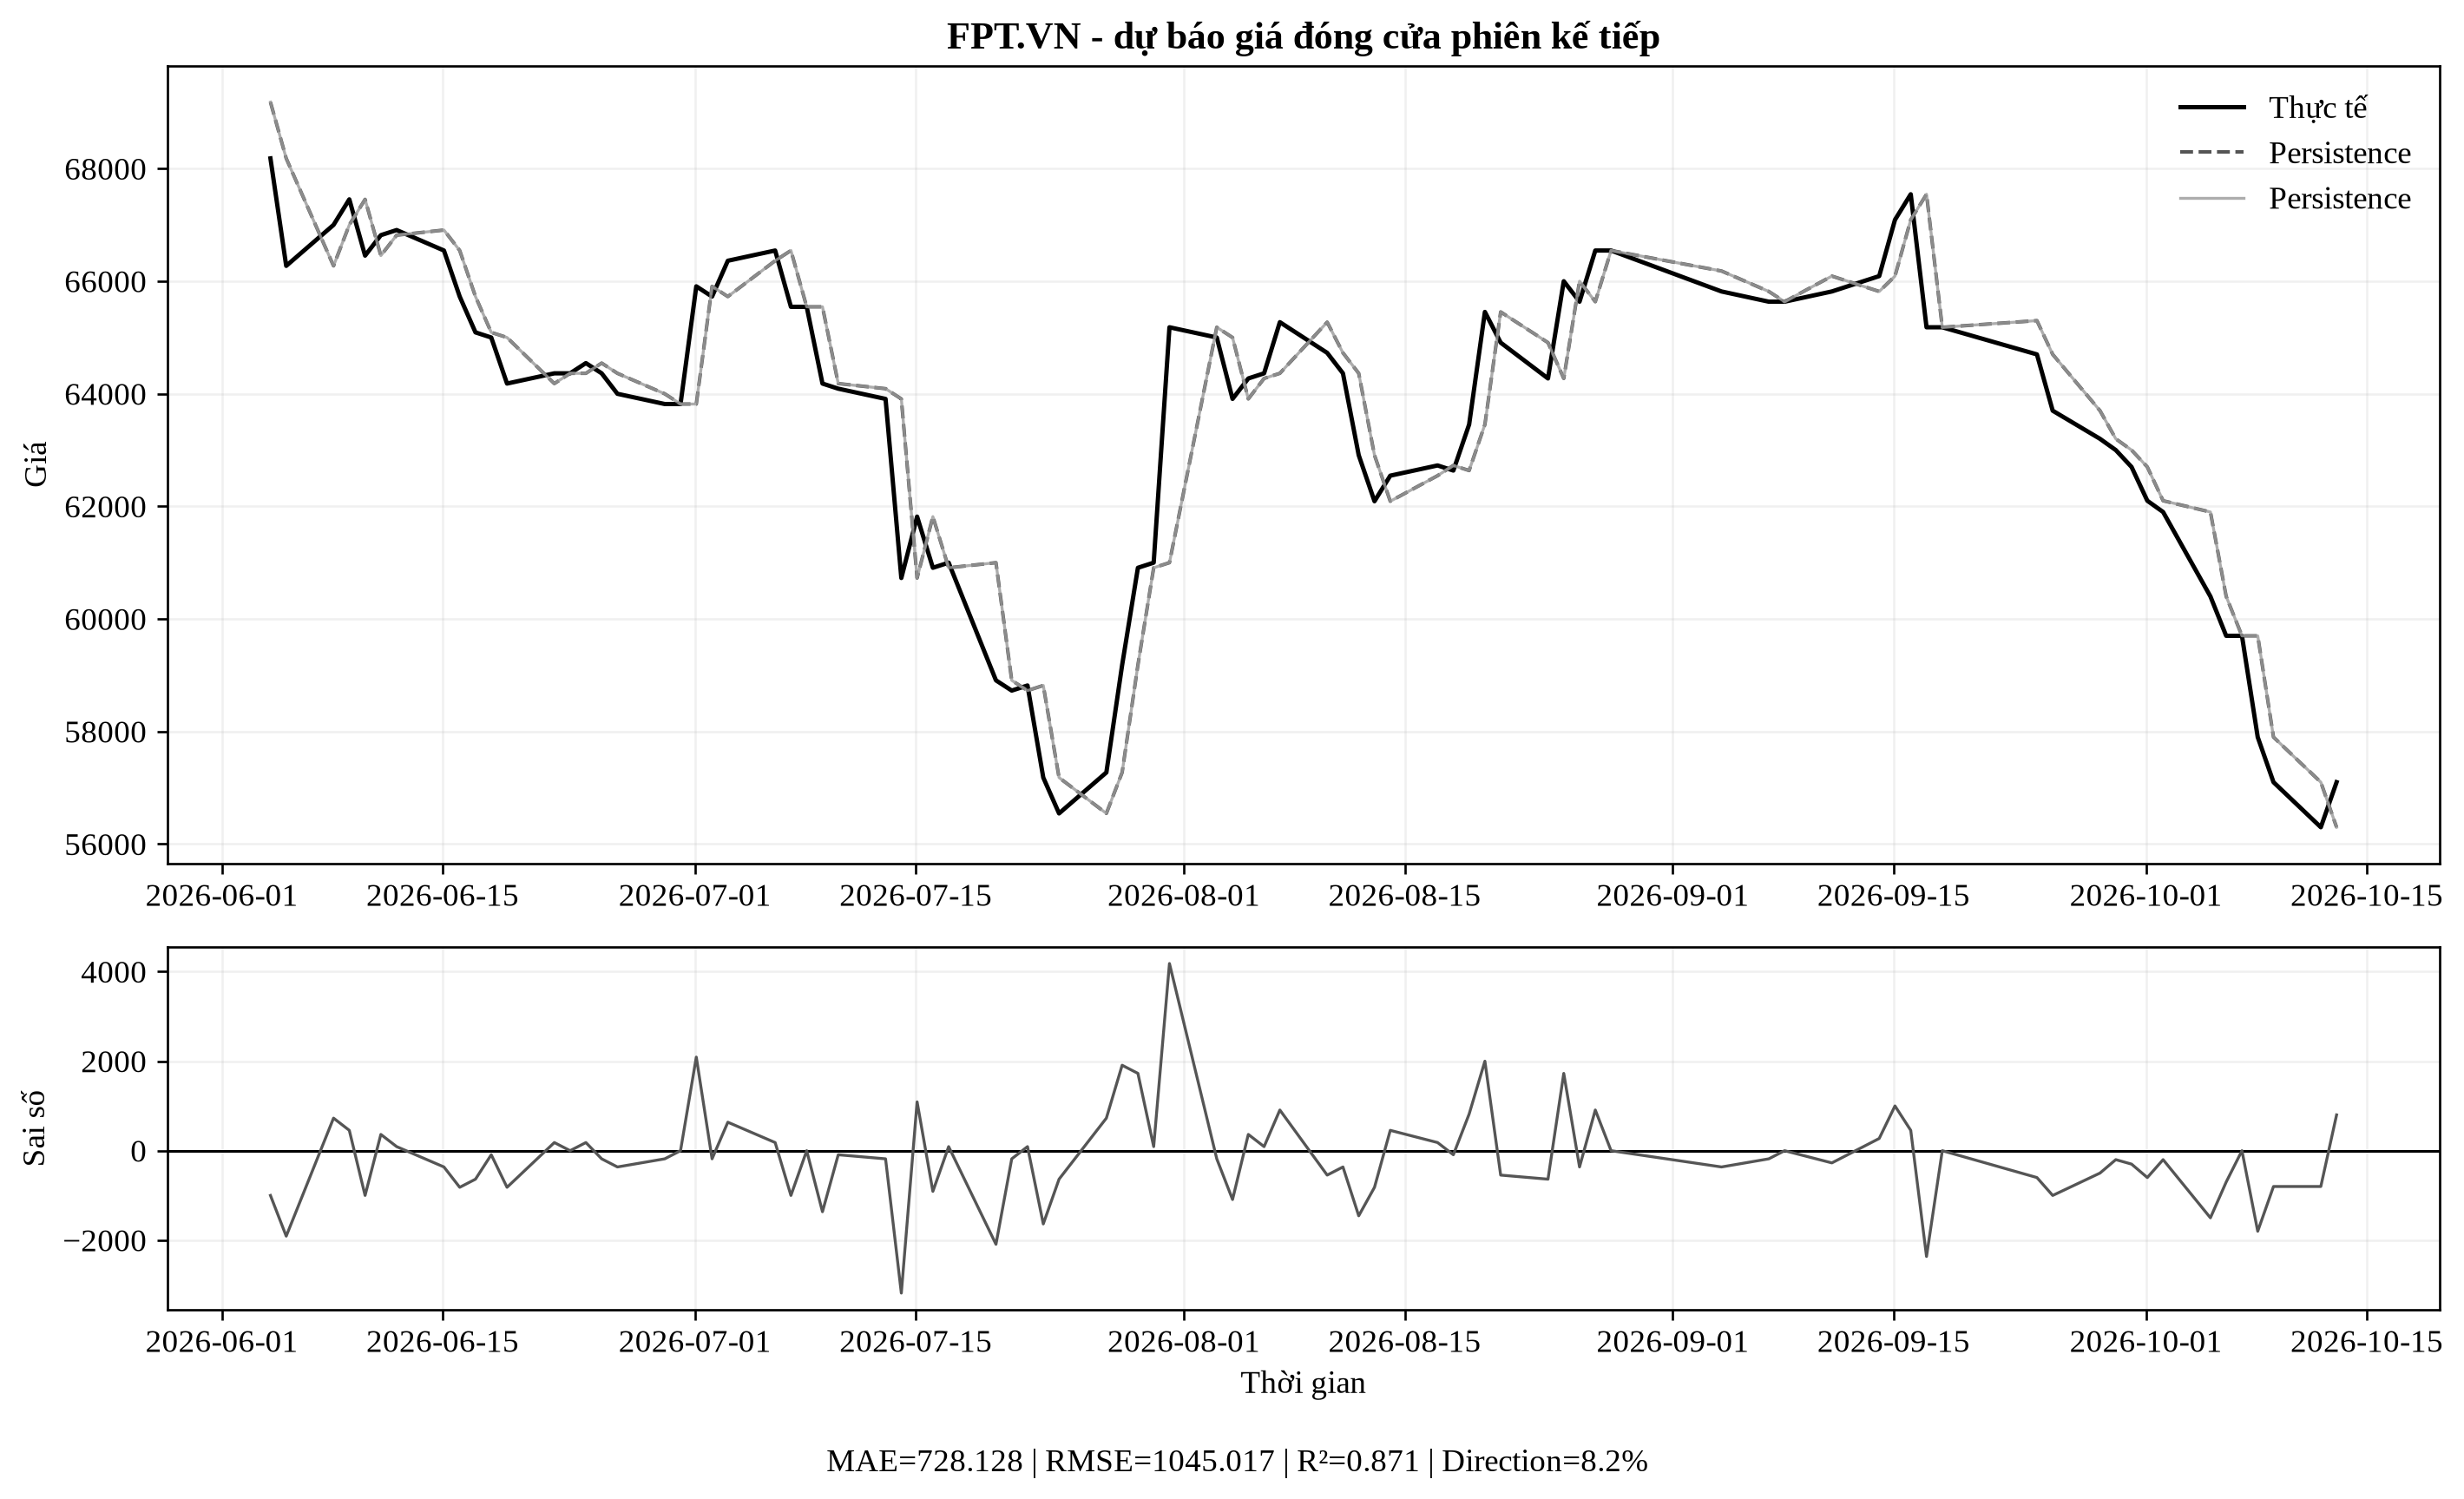
\includegraphics[width=\linewidth,height=.56\textheight,keepaspectratio]{media/media/image35.png}
\caption{Dự báo FPT so với Persistence}\label{fig:legacy-5.14}
\end{figure}



\subsection{Hỏi đáp chứng khoán với GraphRAG}\label{hux1ecfi-ux111uxe1p-chux1ee9ng-khouxe1n-vux1edbi-GraphRAG}

Câu trả lời mẫu: FPT.VN có MA20 62,260, MA60 63,396, RSI14 8.2 và biến
động năm hóa 27.6\%. Đường trung bình động mô tả xu hướng quá khứ chứ
không bảo đảm giá tương lai. RSI là chỉ báo động lượng và cần kết hợp
thanh khoản, cơ bản doanh nghiệp cùng bối cảnh thị trường. Quan hệ đồ
thị liên quan: FPT.VN -{[}CÓ\_GIÁ\_GẦN\_NHẤT{]}→ Giá FPT 57,100 VND;
MA20 -{[}MÔ\_TẢ\_XU\_HƯỚNG\_NGẮN\_HẠN\_CỦA{]}→ FPT.VN; MA60
-{[}MÔ\_TẢ\_XU\_HƯỚNG\_TRUNG\_HẠN\_CỦA{]}→ FPT.VN. Đây là phân tích dữ
liệu quá khứ, không phải khuyến nghị mua hoặc bán.

Tài liệu cung cấp số liệu động; đồ thị giải thích vai trò của chỉ báo và
liên kết multi-hop. Bộ lọc domain ngăn tài liệu vàng hoặc y tế đi vào
câu trả lời chứng khoán.

Kết quả mô hình được ghi thành tài liệu trong KB với model name, thời
gian, MAE và R2. Vì vậy RAG có thể dẫn lại đúng lần huấn luyện thay vì
tạo ra độ chính xác không tồn tại.

\begin{figure}[H]
\centering
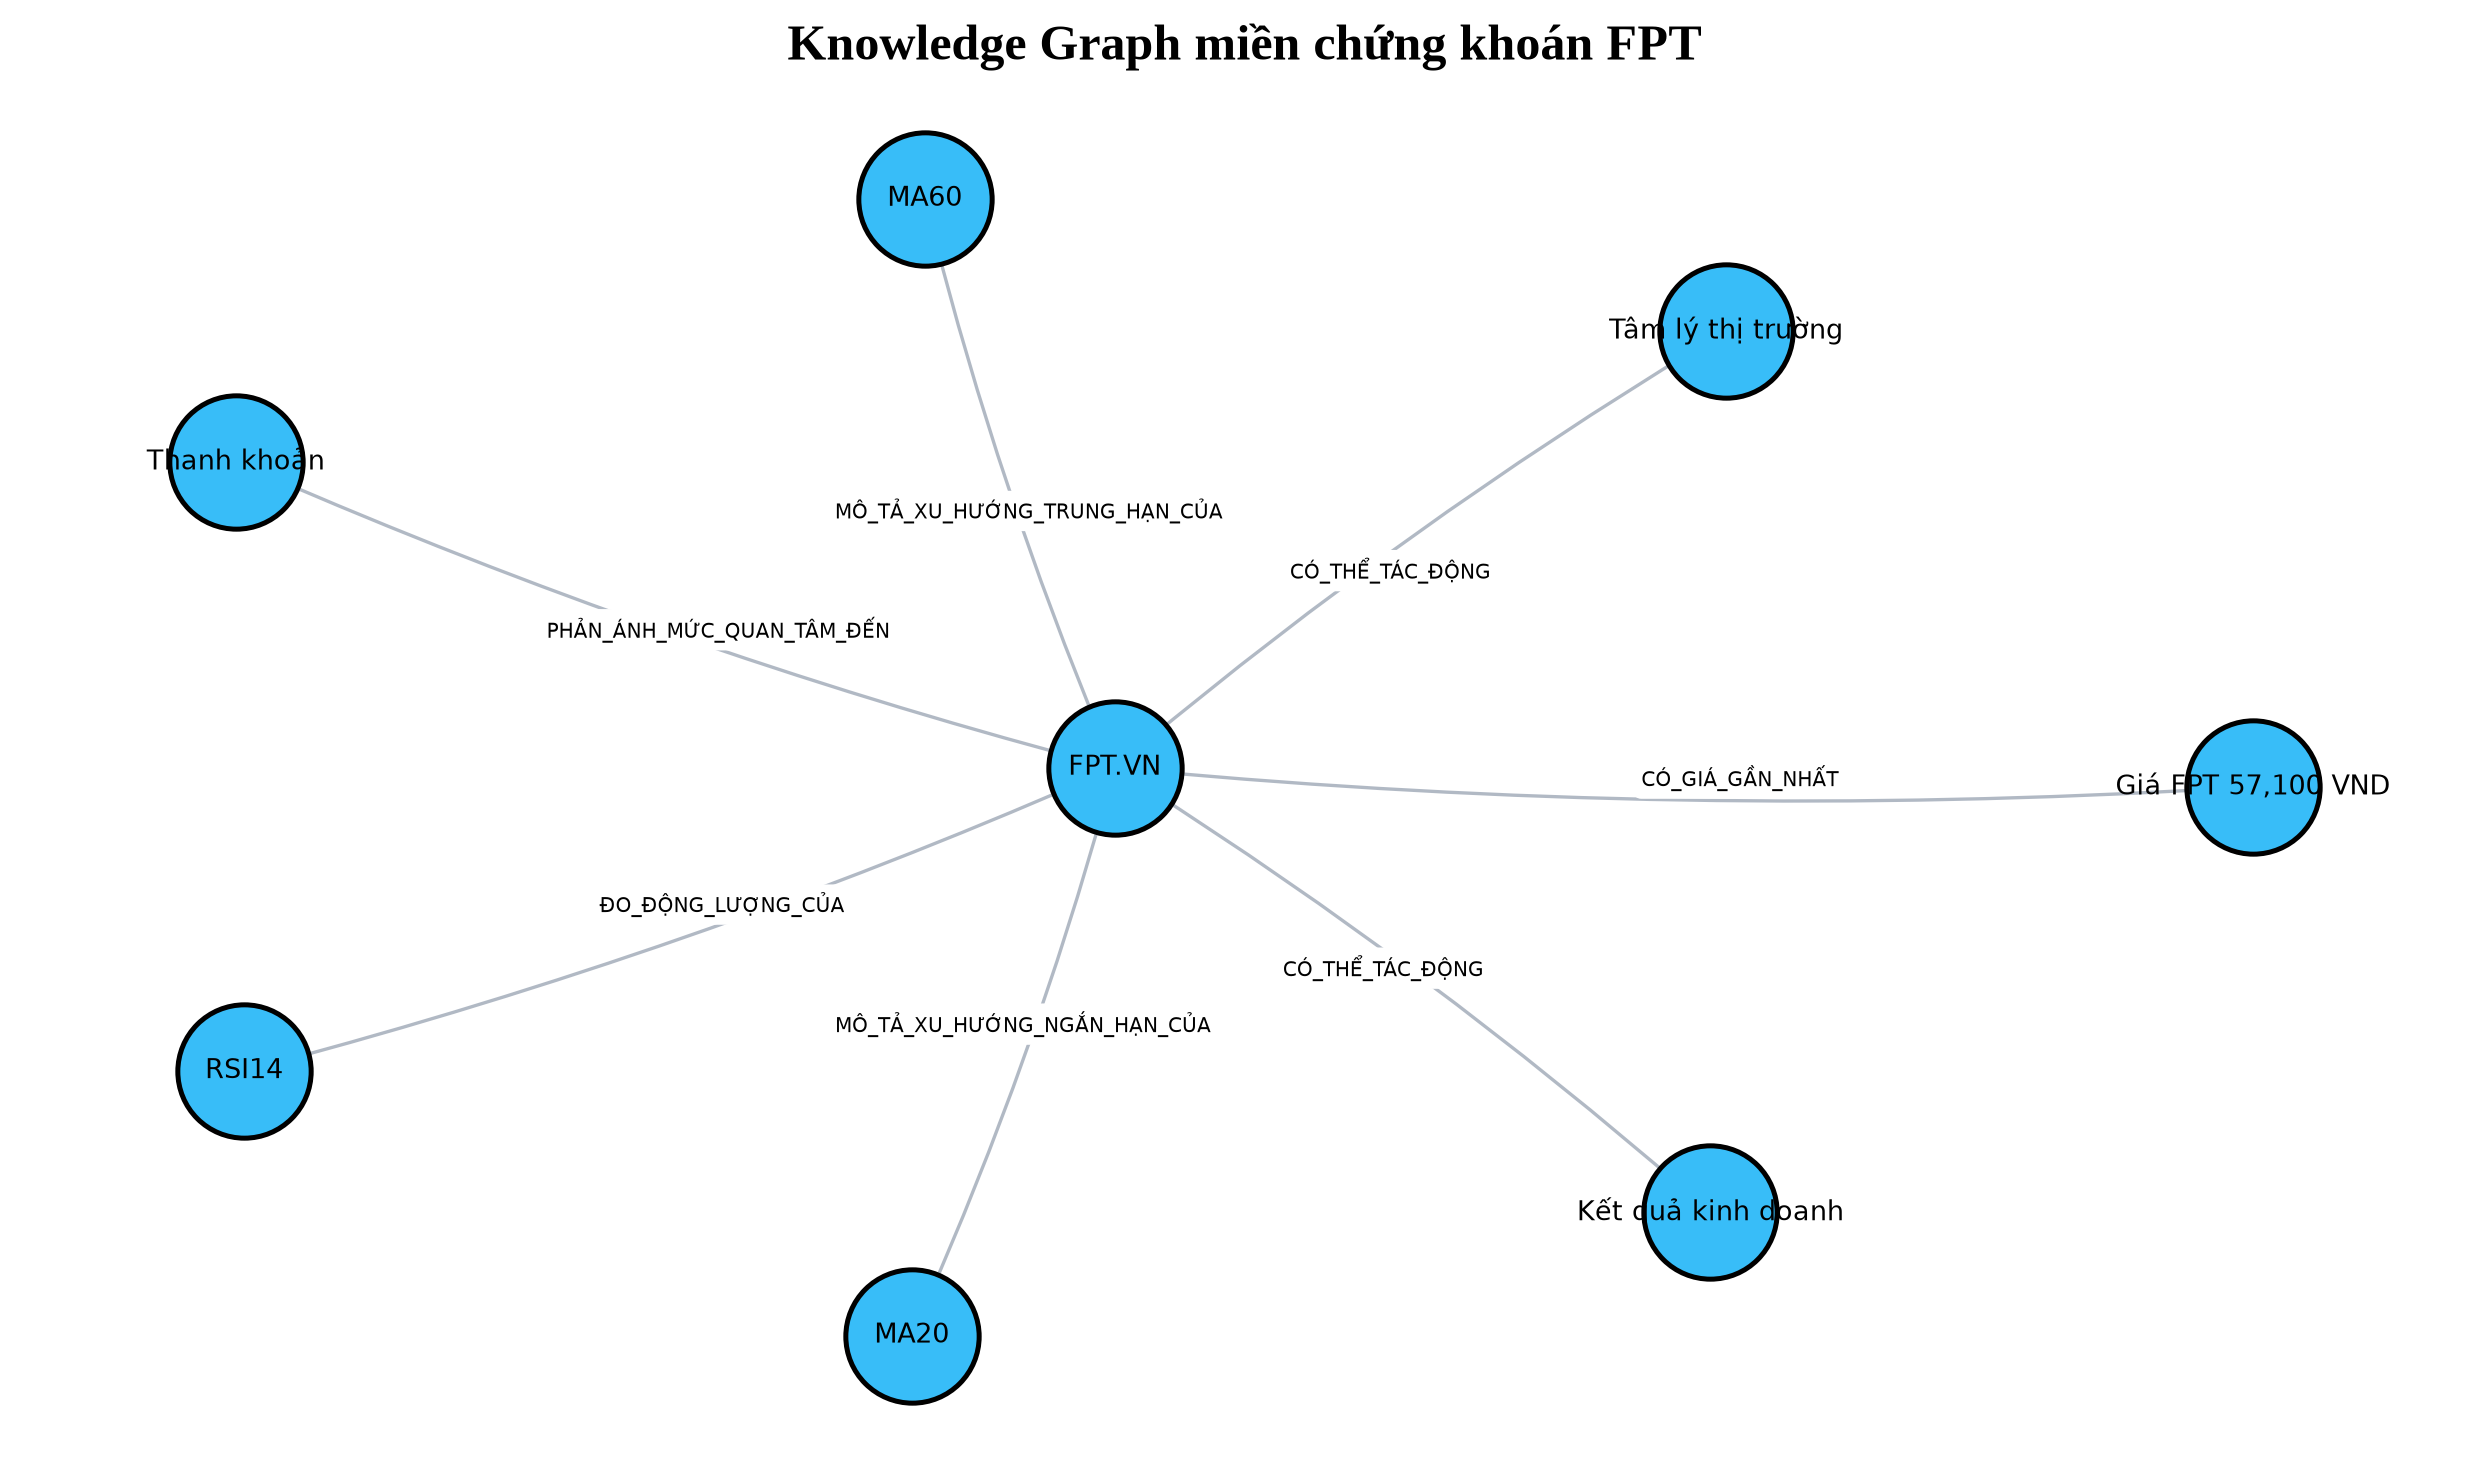
\includegraphics[width=\linewidth,height=.56\textheight,keepaspectratio]{media/media/image36.png}
\caption{Đồ thị tri thức chứng khoán}\label{fig:legacy-5.15}
\end{figure}



\subsection{Rủi ro và hướng mở rộng}\label{rux1ee7i-ro-vuxe0-hux1b0ux1edbng-mux1edf-rux1ed9ng}

Corporate actions, thanh khoản, cách điều chỉnh giá và survivorship bias
có thể làm sai phân tích. Yahoo Finance phù hợp bài tập nhưng nên đối
chiếu nguồn chính thức nếu dùng trong nghiên cứu giao dịch.

Dự báo Close phiên kế tiếp thường có R2 cao do giá hôm nay gần giá ngày
mai; vì vậy phải đọc cùng persistence baseline và directional accuracy.
R2 cao không đồng nghĩa chiến lược có lợi nhuận.

Hướng mở rộng là walk-forward backtest có phí, trượt giá, khoảng tin cậy
và kiểm tra thay đổi chế độ thị trường. Mọi đầu ra vẫn cần cảnh báo
không phải khuyến nghị đầu tư.

\section{KB và RAG cho giá vàng}\label{KB-vuxe0-RAG-cho-giuxe1-vuxe0ng}

Dữ liệu hợp đồng vàng GC=F được lấy từ Yahoo Finance chart API - GC=F.
Khoảng 15/10/2021 - 14/10/2026 có 1257 quan sát; giá gần nhất 4,107.90
USD/oz.

Lợi suất toàn kỳ 132.31\%, biến động năm hóa 19.07\%, RSI14 31.6. GC=F
là tham chiếu quốc tế, không đồng nhất với giá vàng miếng SJC.

Knowledge Graph mô tả lãi suất Fed, USD, lạm phát, địa chính trị và nhu
cầu trú ẩn. Những cạnh này là khung giải thích có điều kiện, không phải
quan hệ nhân quả cố định.

\begin{figure}[H]
\centering
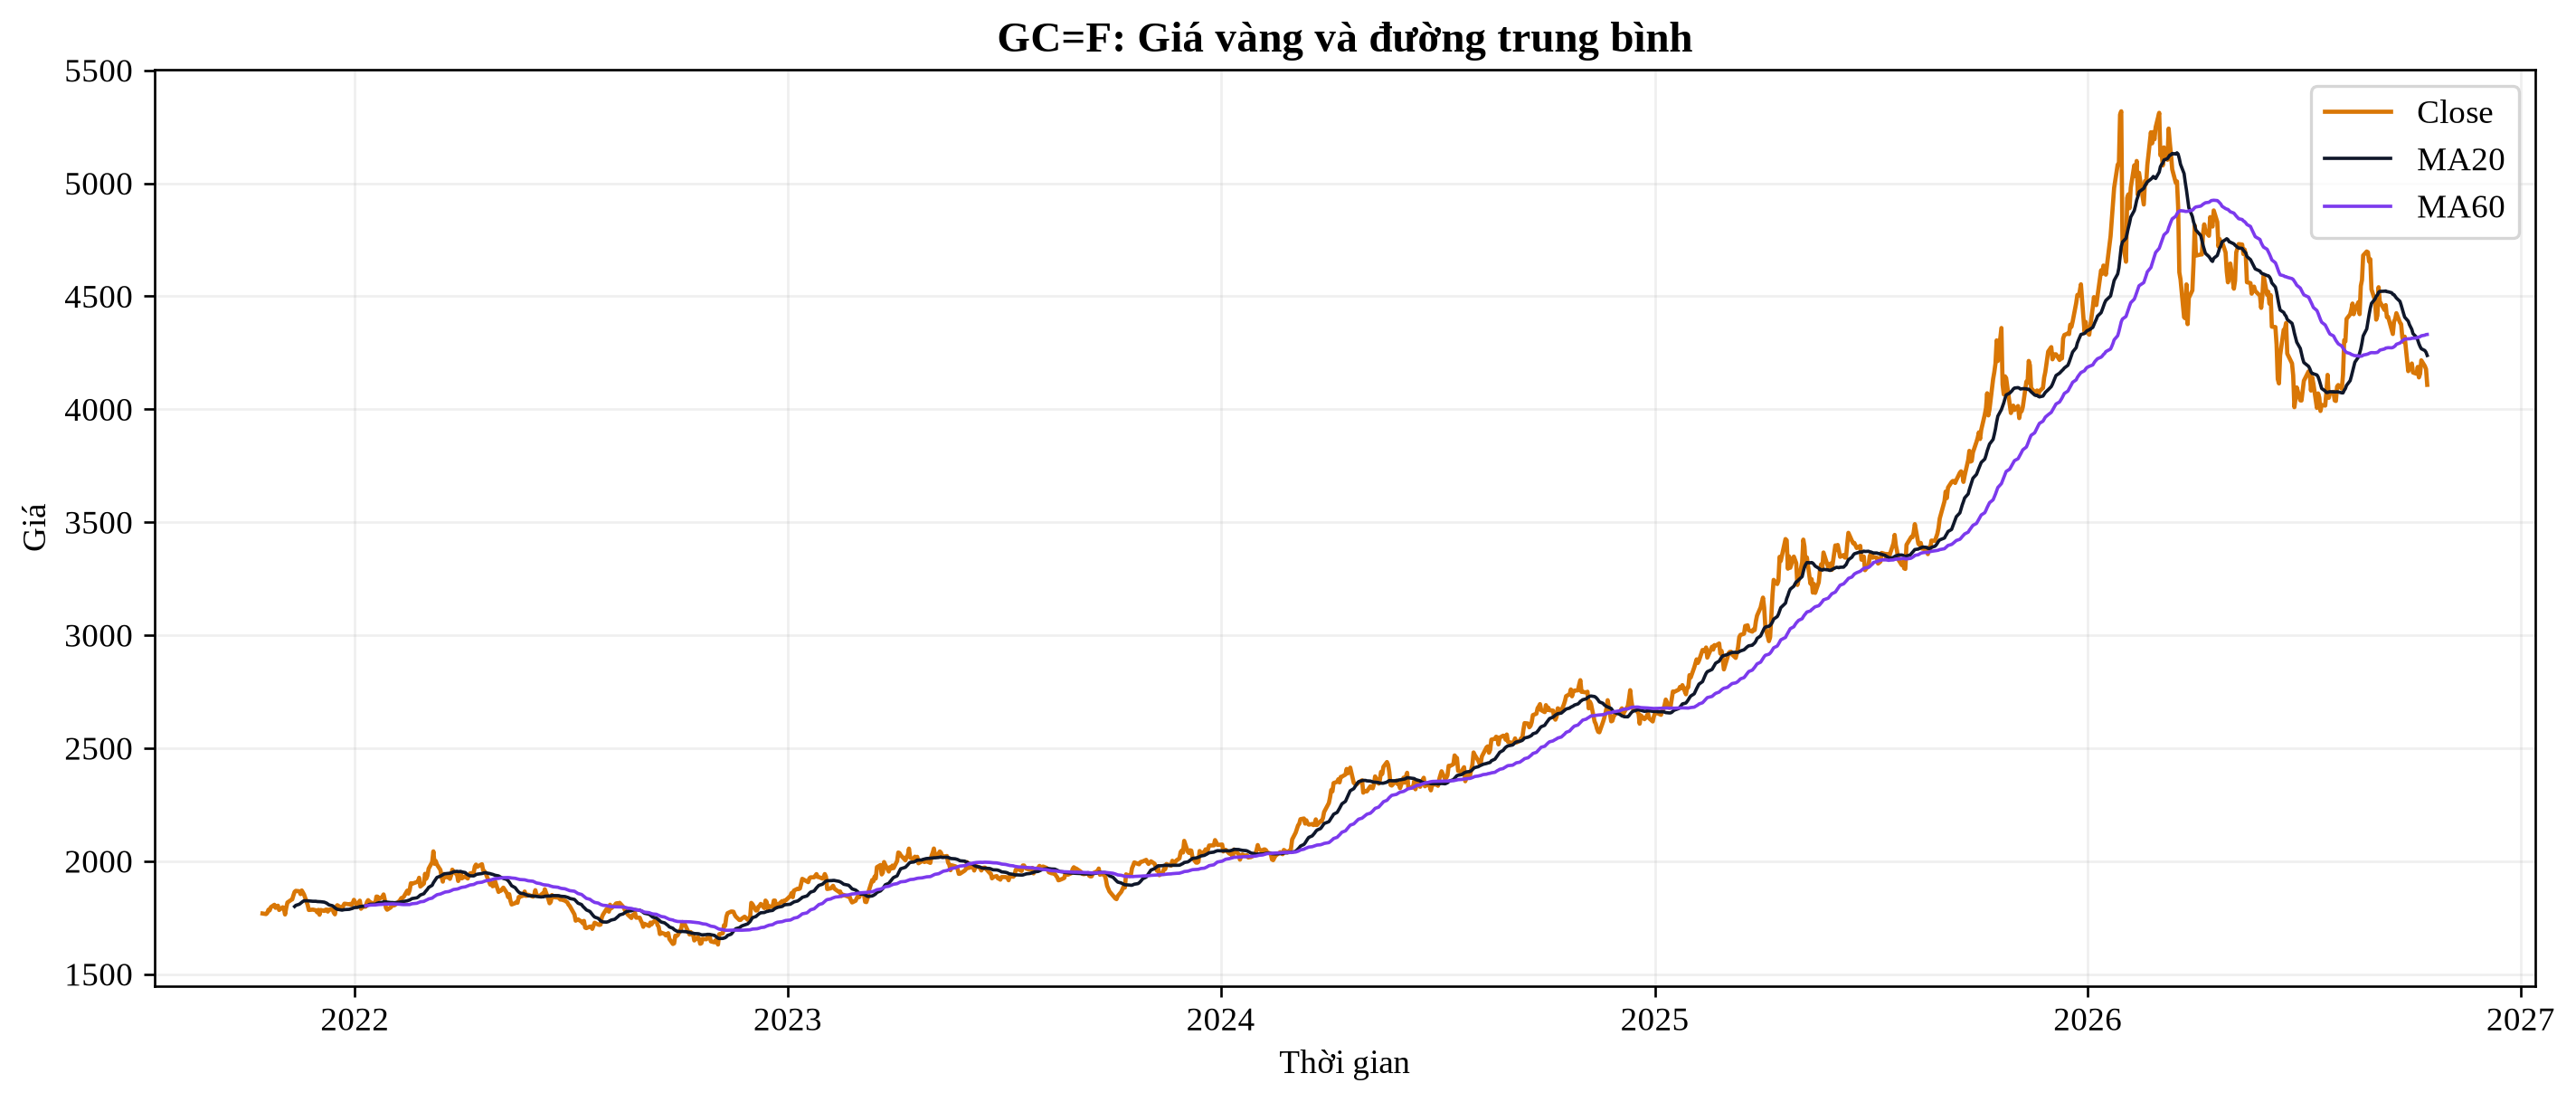
\includegraphics[width=\linewidth,height=.56\textheight,keepaspectratio]{media/media/image37.png}
\caption{Chuỗi giá và chỉ báo vàng}\label{fig:legacy-5.16}
\end{figure}



\subsection{Dữ liệu, chỉ báo và knowledge graph vàng}\label{dux1eef-liux1ec7u-chux1ec9-buxe1o-vuxe0-knowledge-graph-vuxe0ng}

MA20 hiện là 4,237.78, MA60 là 4,330.82. Chuỗi giữ nguyên lịch phiên của
nguồn; không nội suy ngày nghỉ. Biến đích là Close phiên kế tiếp.

Đặc trưng dùng cùng một công thức với FPT để so sánh công bằng: giá và
độ trễ, return, MA20, MA60, volatility20, RSI14, thay đổi volume, biên
độ ngày và chênh lệch Open-Close.

Chuỗi Rủi ro địa chính trị -\textgreater{} Nhu cầu trú ẩn
-\textgreater{} Vàng quốc tế minh họa truy vấn nhiều bước. Quan hệ Vàng
quốc tế -\textgreater{} Giá vàng SJC chỉ là tham chiếu, cần thêm tỷ giá
và cơ chế thị trường trong nước để giải thích chênh lệch.

\begin{figure}[H]
\centering
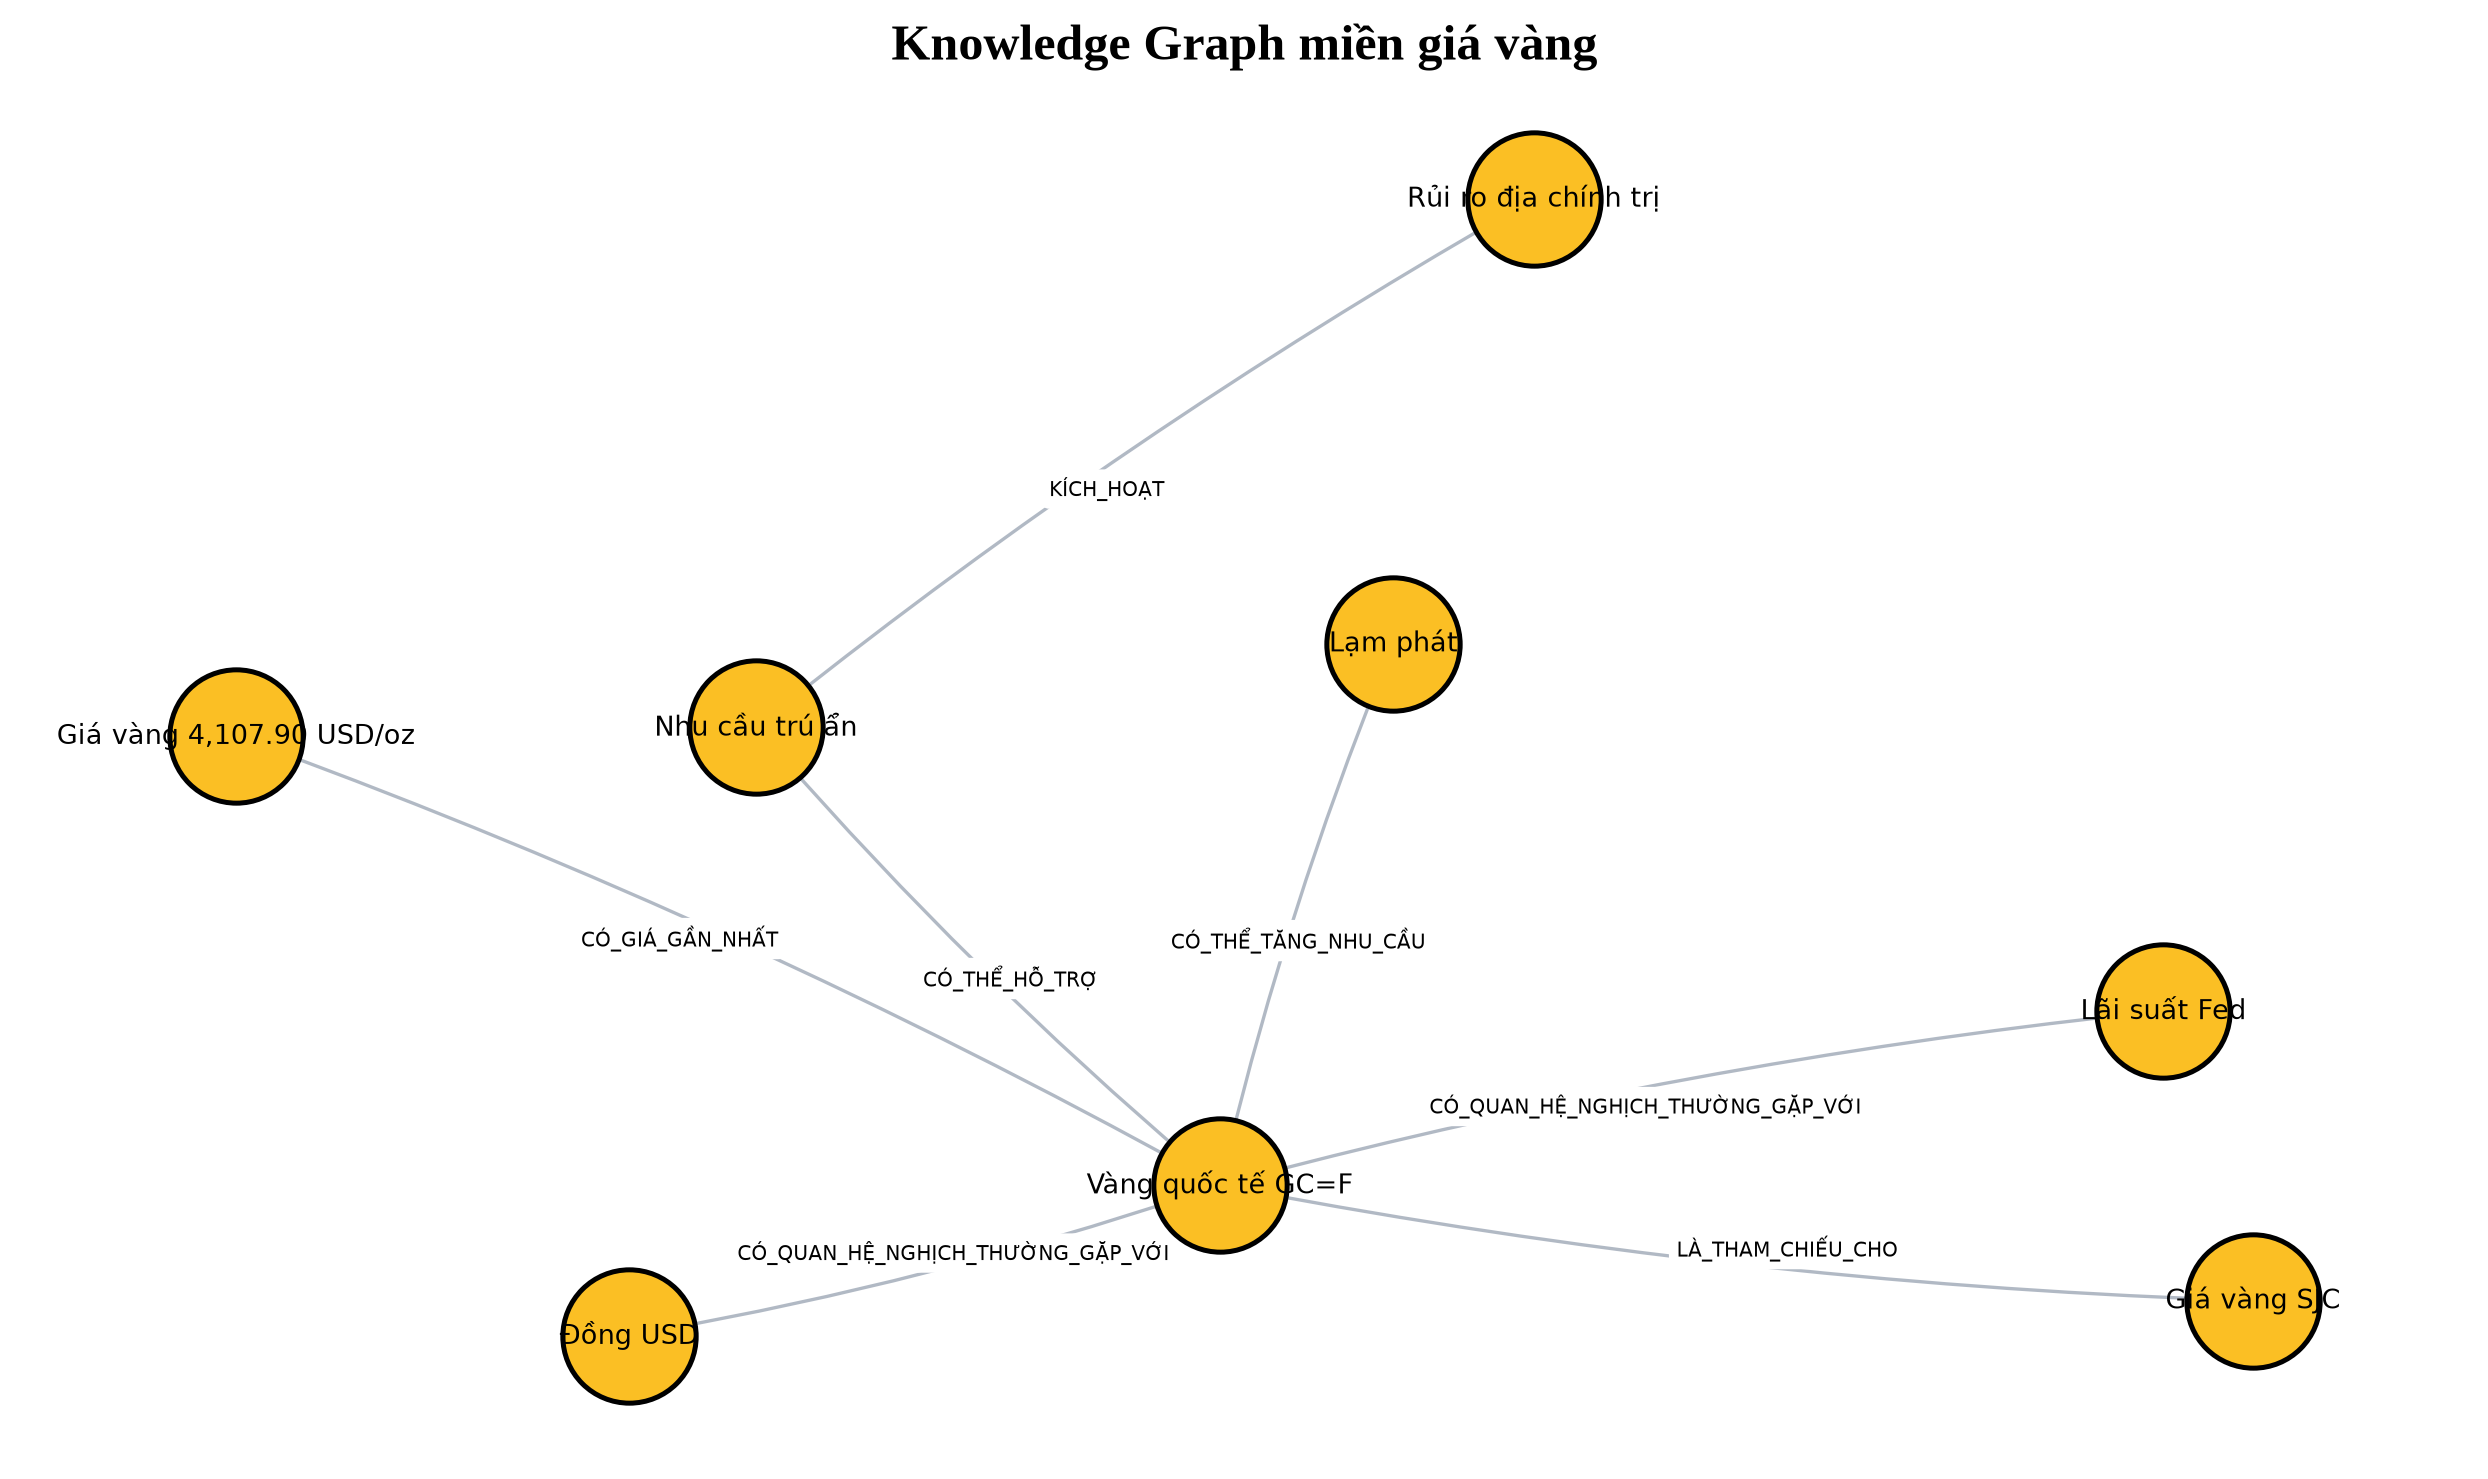
\includegraphics[width=\linewidth,height=.56\textheight,keepaspectratio]{media/media/image38.png}
\caption{Đồ thị tri thức vàng}\label{fig:legacy-5.17}
\end{figure}



\subsection{Huấn luyện và đánh giá mô hình vàng}\label{huux1ea5n-luyux1ec7n-vuxe0-ux111uxe1nh-giuxe1-muxf4-huxecnh-vuxe0ng}

Vàng dùng cùng quy trình lựa chọn có baseline và mô hình lợi suất như
FPT. Không ép chọn mô hình phức tạp nếu Persistence có CV MAE thấp hơn.
Train, hiệu chỉnh và test nằm theo đúng thứ tự thời gian, có khoảng cách
một phiên ở ranh giới.

Mô hình được chọn: SVR return; CV MAE 38.792; test MAE 49.440; R2 0.880.
Baseline MAE 48.267; cải thiện -2.43\%.

Test từ 2026-06-09 đến 2026-10-13; bản trước có MAE 50.4701. Mức giảm
sai số so với bản trước là 2.04\%, nhưng vẫn cần đối chiếu baseline.
Khoảng bootstrap khối 5 phiên, 2.000 lần lặp cho mức cải thiện so với
baseline: -6.10\% đến 2.68\%. Khoảng chứa 0 chưa chứng minh cải thiện rõ
ràng. GC=F không phải vàng SJC.

\begin{figure}[H]
\centering
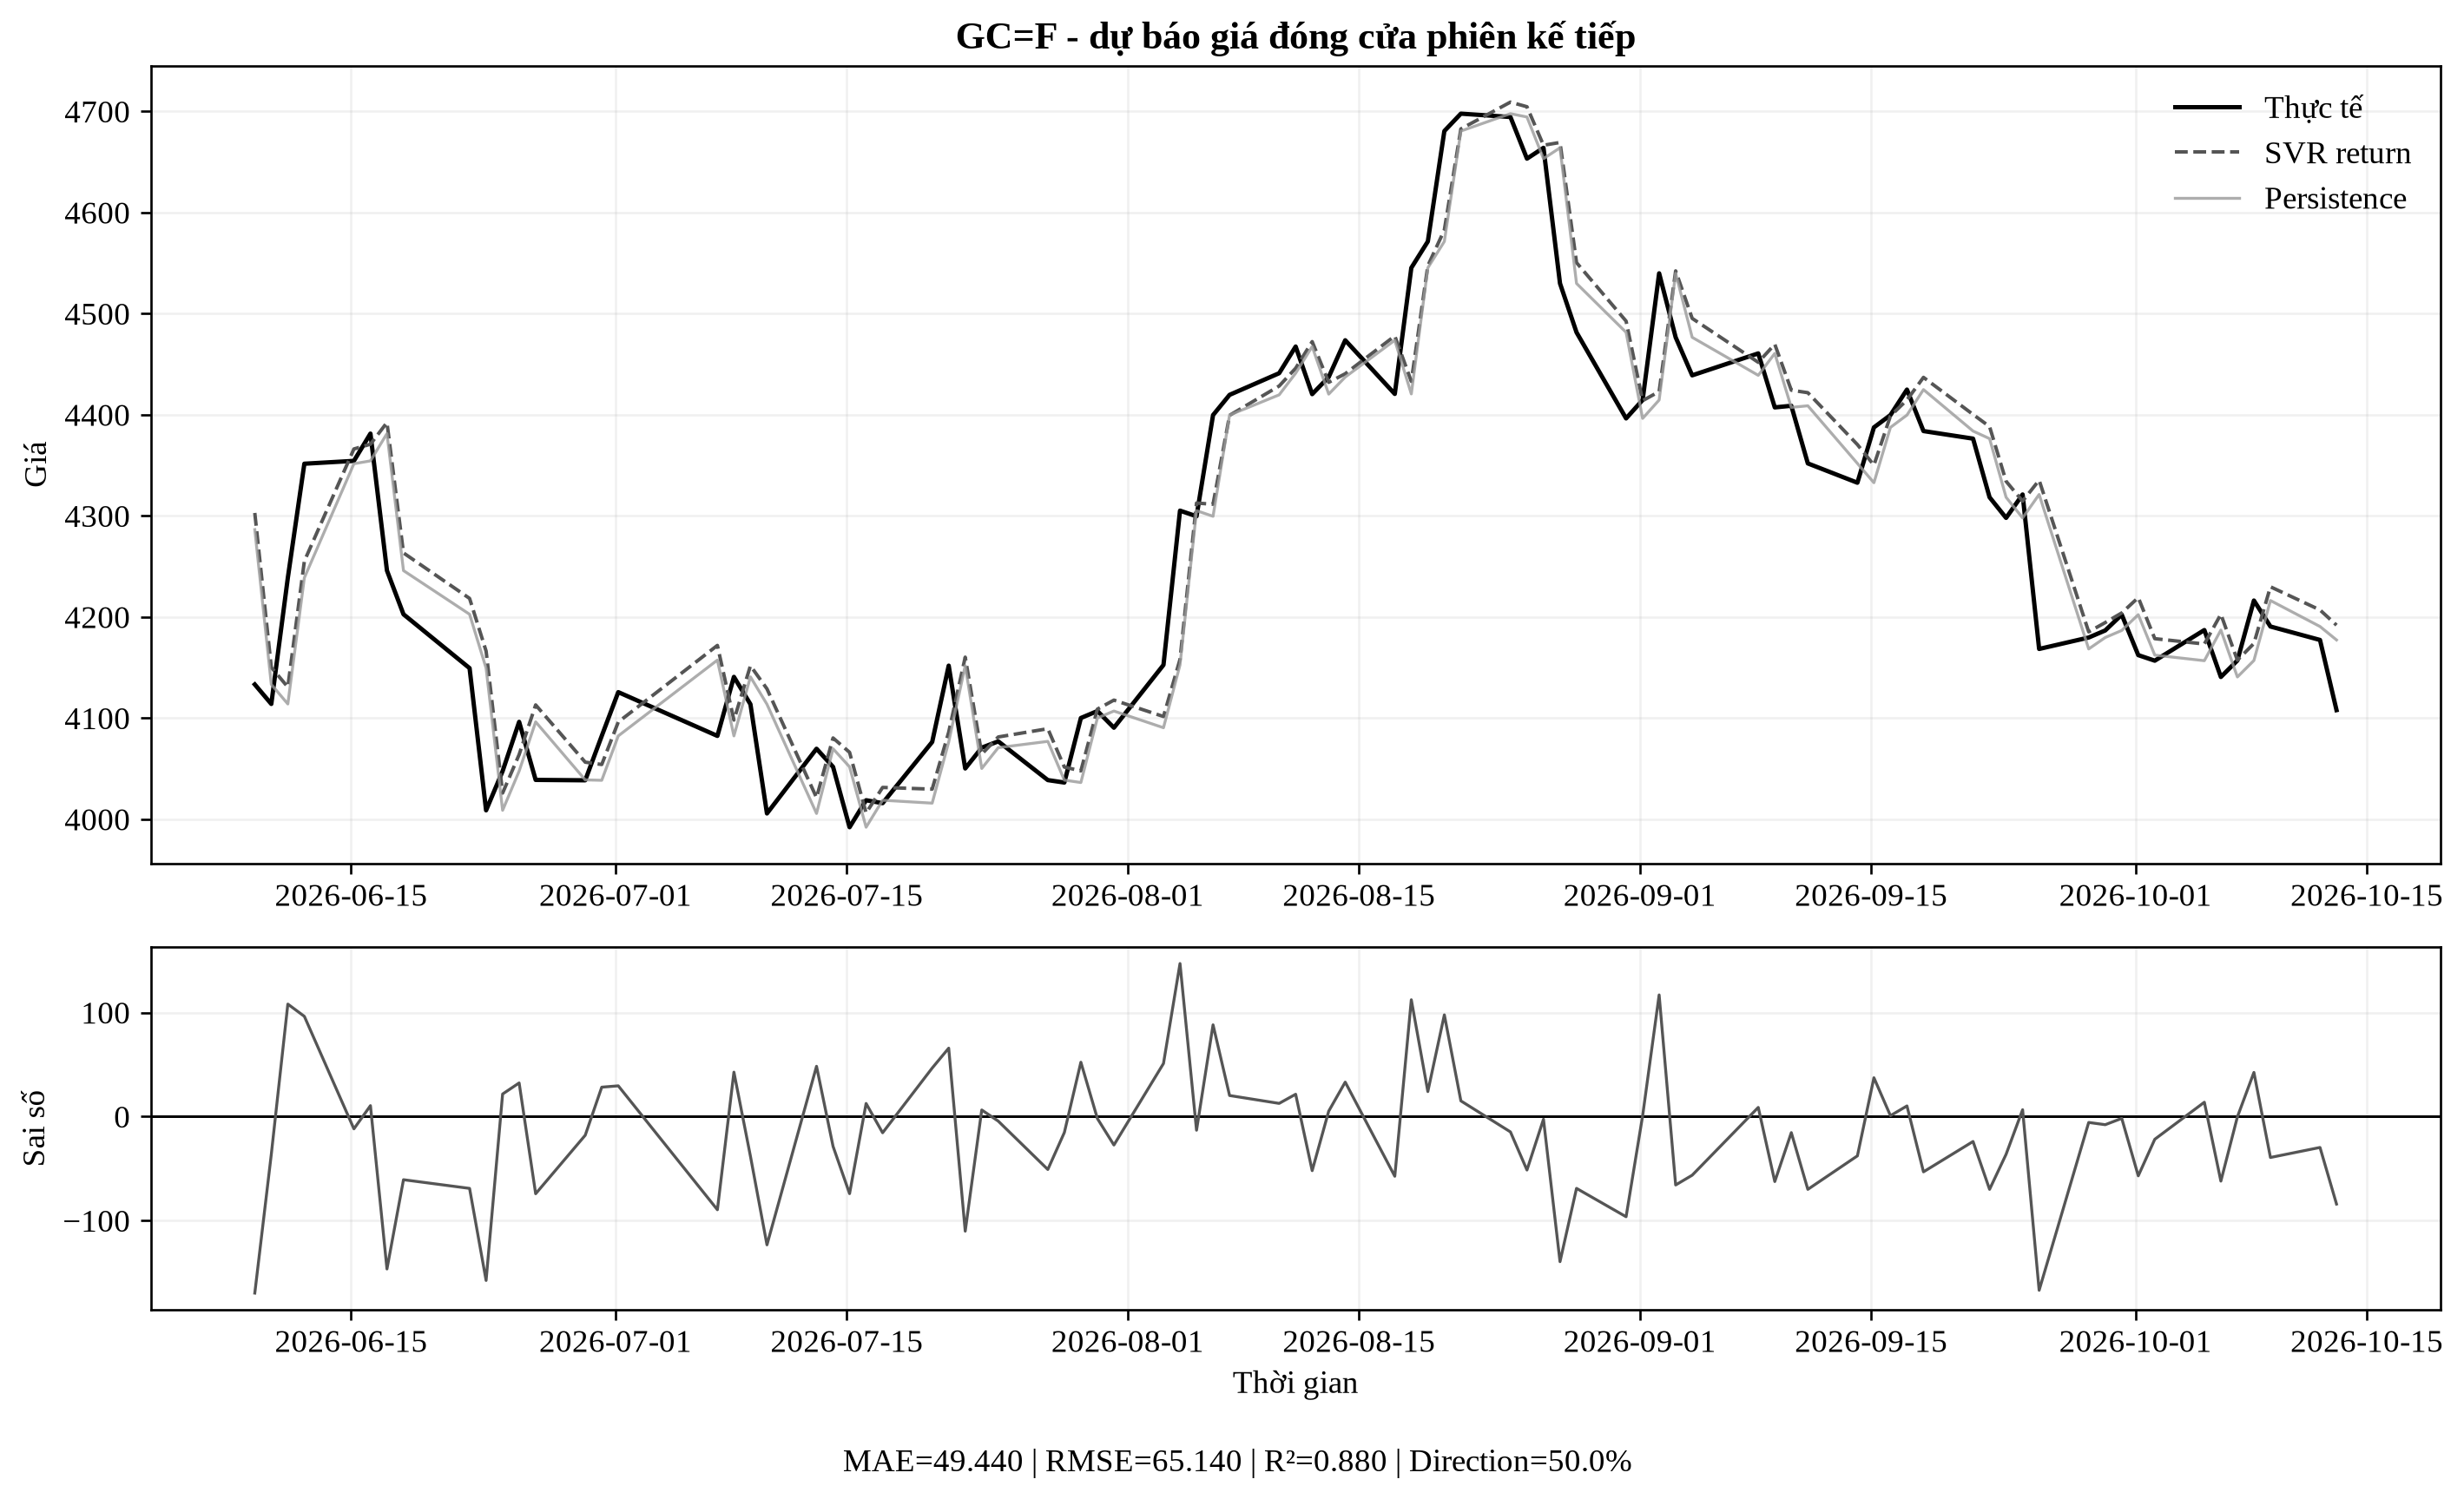
\includegraphics[width=\linewidth,height=.56\textheight,keepaspectratio]{media/media/image39.png}
\caption{Mô hình vàng và baseline}\label{fig:legacy-5.18}
\end{figure}



\subsection{Hỏi đáp vĩ mô với GraphRAG}\label{hux1ecfi-ux111uxe1p-vux129-muxf4-vux1edbi-GraphRAG}

Câu trả lời mẫu: Giá vàng thường nhạy với lãi suất thực, sức mạnh đồng
USD, kỳ vọng lạm phát, nhu cầu dự trữ và rủi ro địa chính trị; quan hệ
có thể thay đổi theo từng giai đoạn. Chuỗi vàng GC=F gồm 1257 phiên từ
15/10/2021 đến 14/10/2026; giá gần nhất 4,107.90 USD/oz. Quan hệ đồ thị
liên quan: Vàng quốc tế GC=F -{[}CÓ\_GIÁ\_GẦN\_NHẤT{]}→ Giá vàng
4,107.90 USD/oz; Vàng quốc tế GC=F -{[}LÀ\_THAM\_CHIẾU\_CHO{]}→ Giá vàng
SJC; Lãi suất Fed -{[}CÓ\_QUAN\_HỆ\_NGHỊCH\_THƯỜNG\_GẶP\_VỚI{]}→ Vàng
quốc tế GC=F. Đây là phân tích dữ liệu quá khứ, không phải khuyến nghị
mua hoặc bán.

Truy xuất văn bản nêu điều kiện và độ bất định; đồ thị cung cấp các cạnh
thường gặp và đường đi qua nhu cầu trú ẩn. Hai nguồn bằng chứng cùng
xuất hiện giúp câu trả lời tránh tuyệt đối hóa.

Nếu thay bộ sinh mẫu bằng LLM, prompt phải cấm tự tạo mục tiêu giá hoặc
xác suất tăng giảm khi evidence không cung cấp. Citation ID và timestamp
nên là trường bắt buộc trong JSON đầu ra.

\begin{figure}[H]
\centering
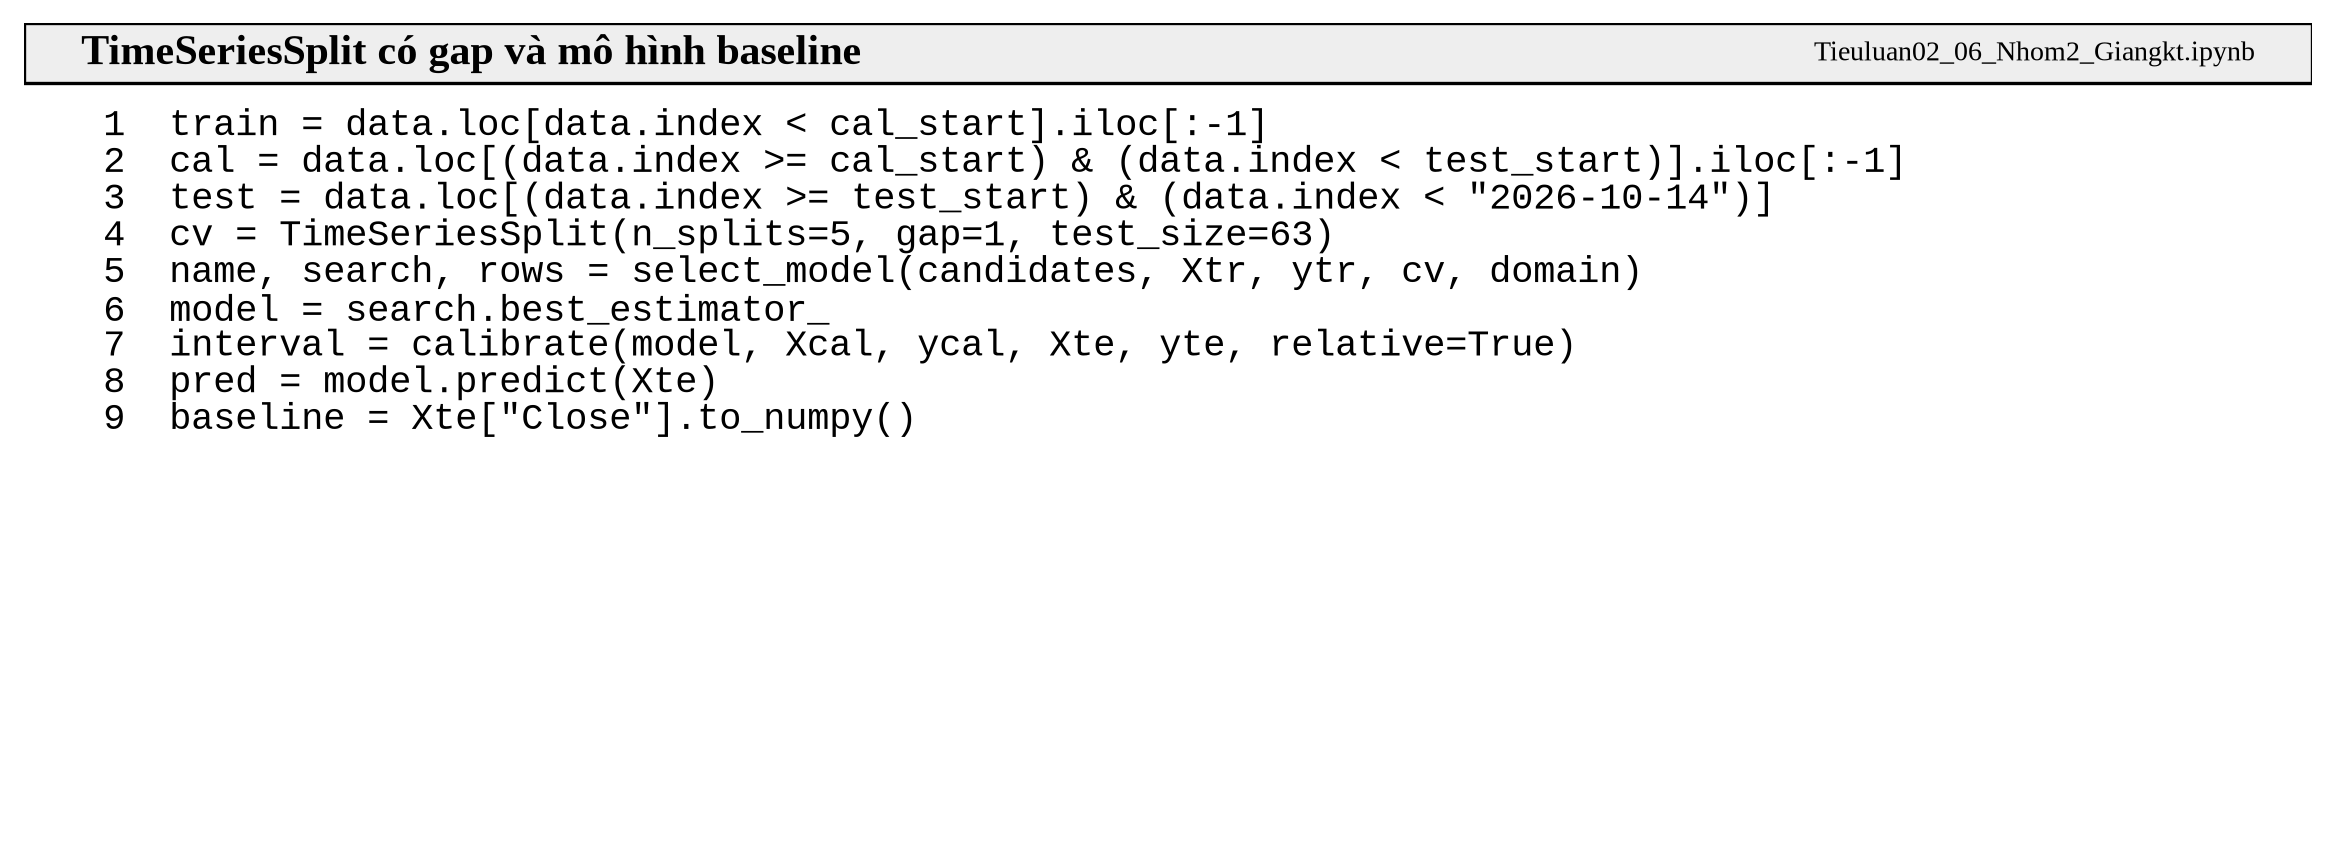
\includegraphics[width=\linewidth,height=.56\textheight,keepaspectratio]{media/media/image40.png}
\caption{Quy trình học máy cho thị trường}\label{fig:legacy-5.19}
\end{figure}



\subsection{Giới hạn và hướng mở rộng}\label{giux1edbi-hux1ea1n-vuxe0-hux1b0ux1edbng-mux1edf-rux1ed9ng}

Hợp đồng tương lai có ngày đáo hạn và cơ chế nối chuỗi. Spot XAU/USD,
futures GC=F và vàng SJC là ba sản phẩm khác nhau; không thể trộn USD/oz
với VND/lượng nếu chưa quy đổi.

Mô hình hiện chưa dùng lãi suất thực, DXY, tỷ giá USD/VND hay vị thế
ETF. Hướng mở rộng là gắn timestamp cho các yếu tố vĩ mô, thử độ trễ và
lưu confidence cùng evidence trên mỗi cạnh.

Tương tự chứng khoán, dự báo một bước chỉ minh họa quy trình machine
learning có kiểm soát. Nó không phải khuyến nghị mua, bán hay nắm giữ
vàng.

\section{Deployment}\label{deployment}

Insight Lab 2.0 chia thành khu Dự đoán với ba tab Tiểu đường, FPT, Vàng
và khu Trợ lý sức khỏe riêng. Người dùng xem kết quả tại từng tab; khi
muốn thảo luận, chủ động chọn chia sẻ kết quả sức khỏe cho chatbot.

Web hiển thị biểu đồ lịch sử giá, dự báo điểm, khoảng sai số hiệu chỉnh
và so sánh baseline. Đầu vào trống, sai đơn vị hoặc vượt giới hạn được
kiểm tra trước suy luận. Giá trị ngoài phạm vi train được đánh dấu để
tránh hiểu sai mức tin cậy.

Web: \url{https://rag-httm-chatbot.vercel.app/}

GitHub: \url{https://github.com/jellalaz/HTTM_ThayQue}

Hình bố cục dưới đây là sơ đồ minh họa, không phải ảnh chụp màn hình.

\begin{figure}[H]
\centering
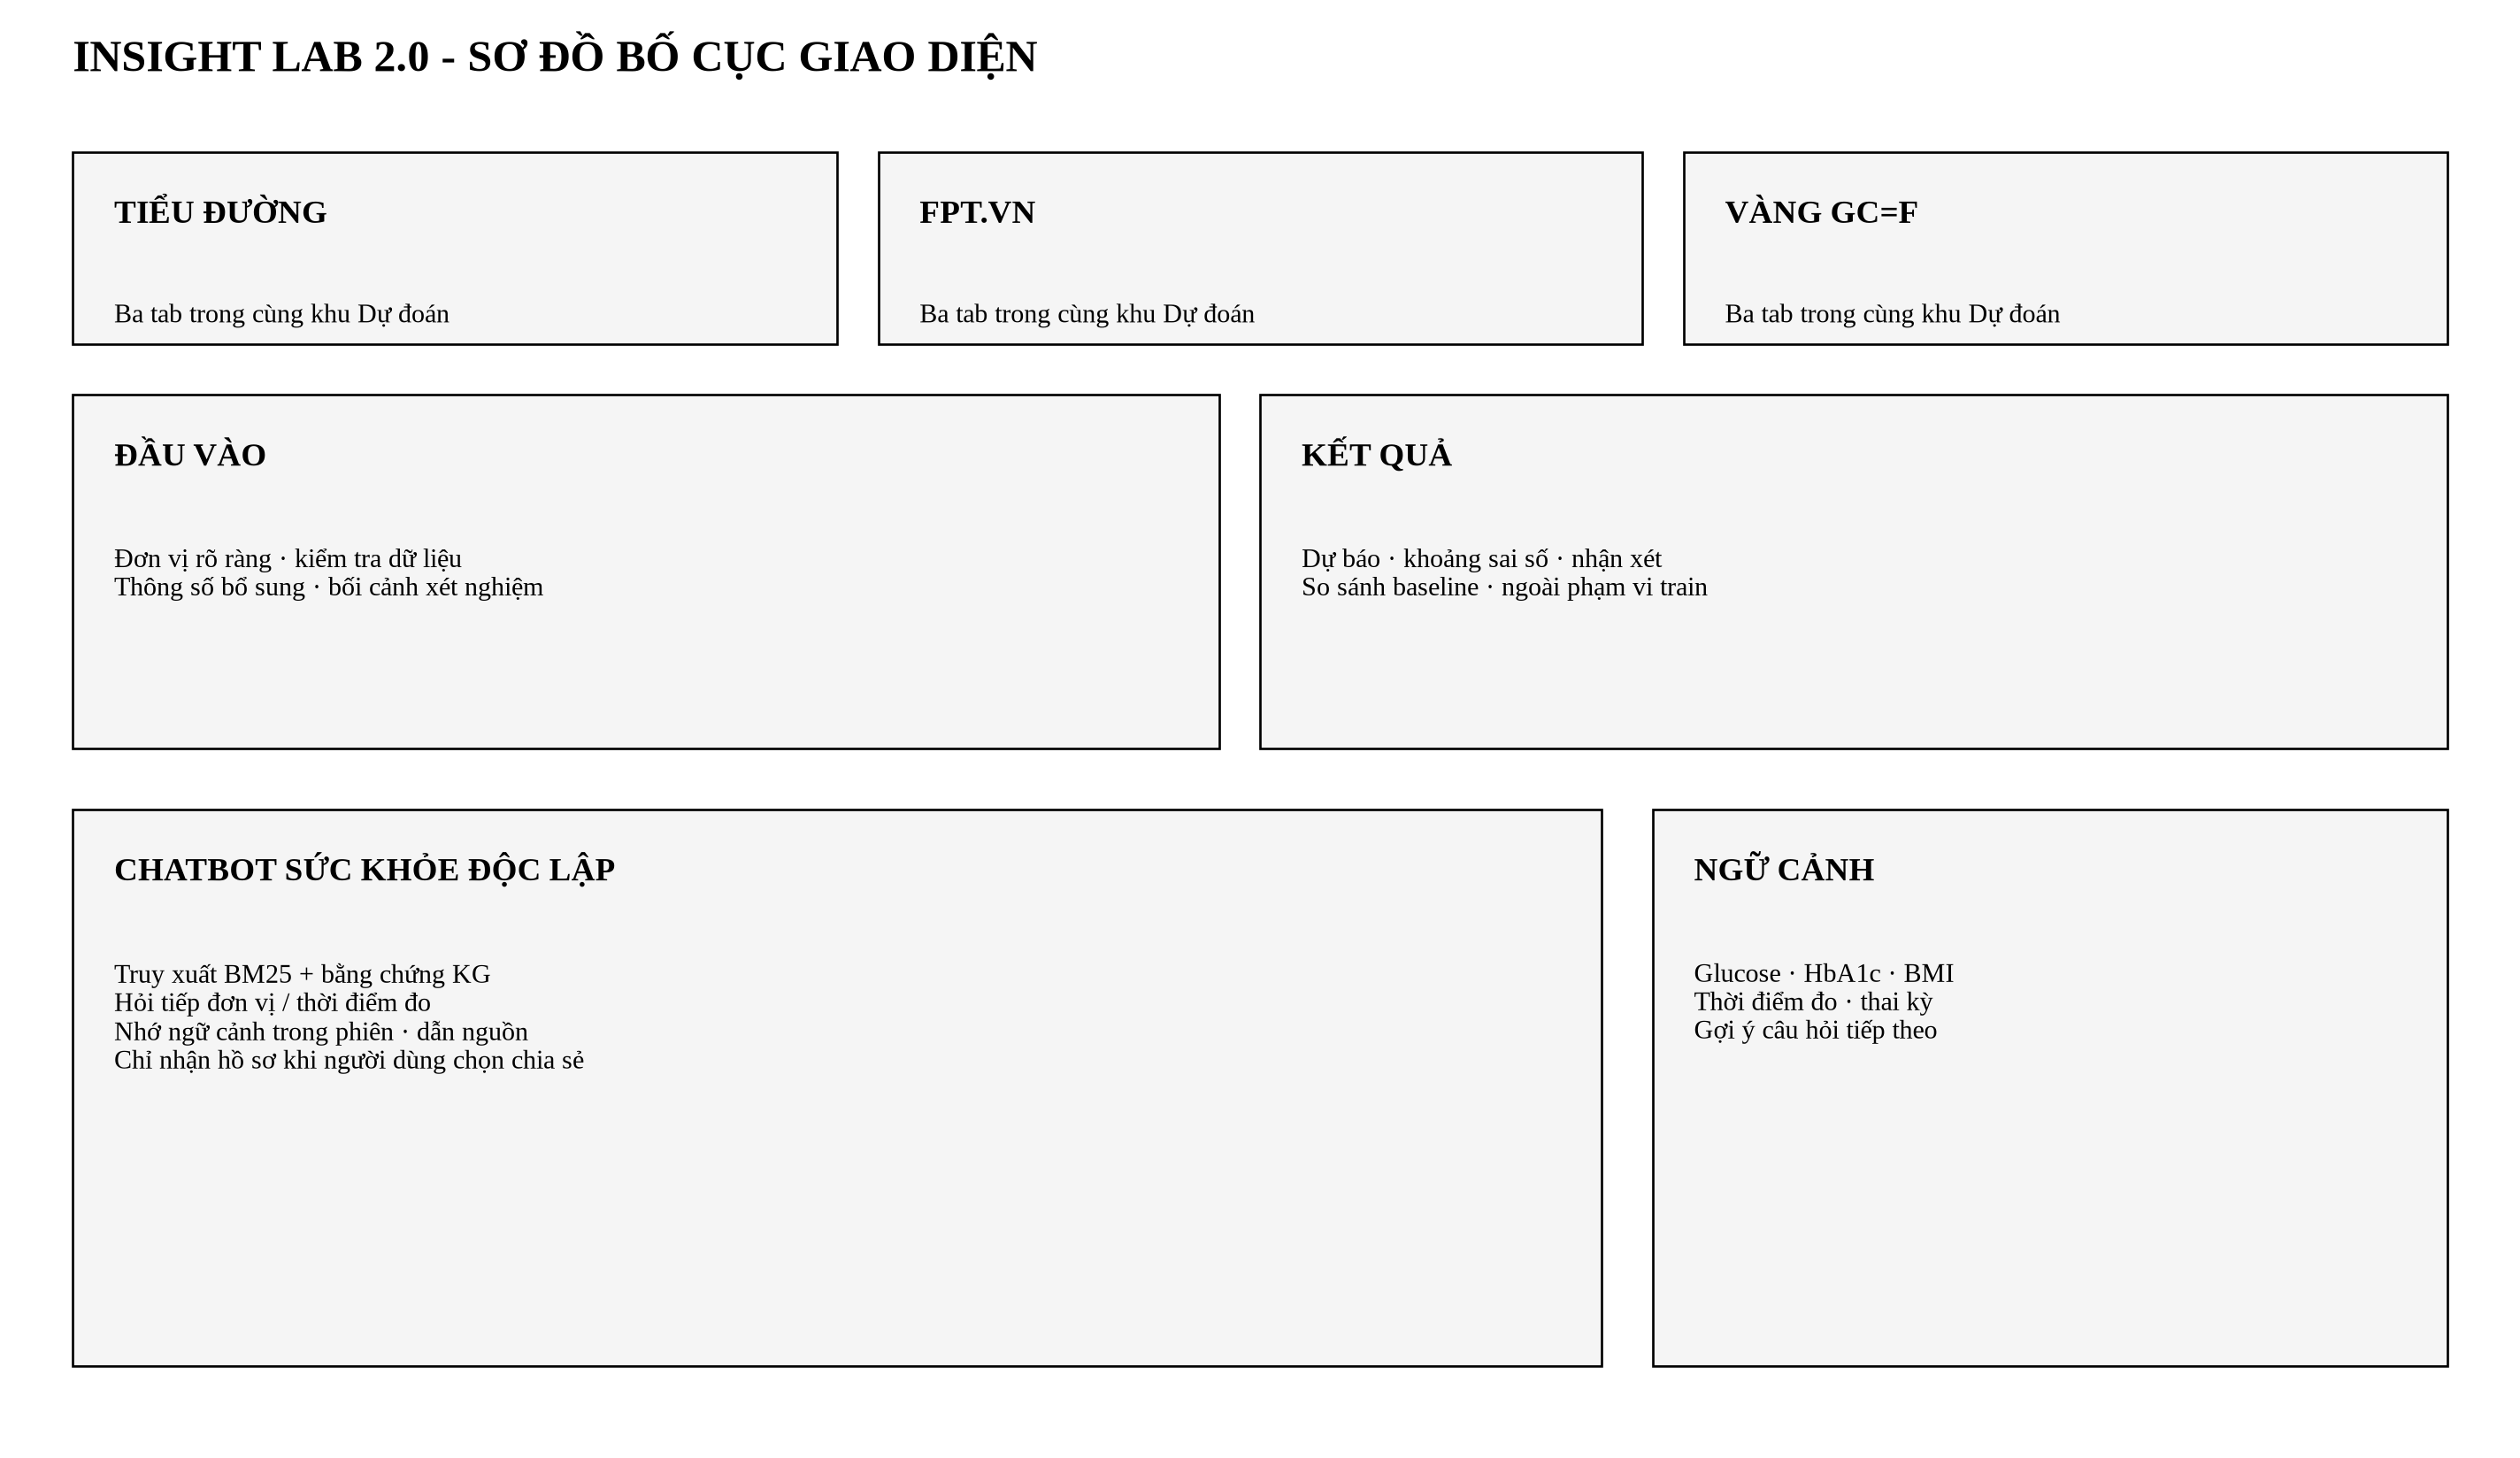
\includegraphics[width=\linewidth,height=.56\textheight,keepaspectratio]{media/media/image41.png}
\caption{Sơ đồ bố cục giao diện gốc}\label{fig:legacy-5.20}
\end{figure}



\subsection{Suy luận mô hình trên trình duyệt}\label{suy-luux1eadn-muxf4-huxecnh-truxean-truxecnh-duyux1ec7t}

Notebook xuất cấu trúc estimator được chọn: scaler, hệ số tuyến tính,
vector hỗ trợ và kernel RBF của SVR, cấu trúc cây hoặc công thức
Persistence/lợi suất. JavaScript dùng cùng đặc trưng và tham số. Các
vector đối chiếu Python/JavaScript được lưu để kiểm tra sai số đóng gói.

Mô hình sức khỏe có sáu trường chính và bốn trường bổ sung. Trường bổ
sung trống dùng trung vị tập train và được công bố ở kết quả. HbA1c và
bối cảnh đo dùng cho nhận xét xét nghiệm riêng, không bị đưa nhầm vào mô
hình chưa học chúng. Điểm tiến triển không được dùng quyết định chẩn
đoán hoặc cấp cứu.

Cấu hình thị trường được chọn trên dữ liệu trước test rồi fit lại cho
web, chừa 63 phiên gần nhất để hiệu chỉnh khoảng dự báo và bỏ cách một
phiên. Chỉ số test lịch sử thuộc bản fit trước đó, không phải đánh giá
ngoài mẫu của bản refit. Web hiển thị riêng hai giai đoạn. Cảnh báo
ngoài miền của mô hình lợi suất xét đặc trưng tương đối, không chỉ mức
giá tuyệt đối. Web không gửi hồ sơ sức khỏe ra ngoài.

\begin{figure}[H]
\centering
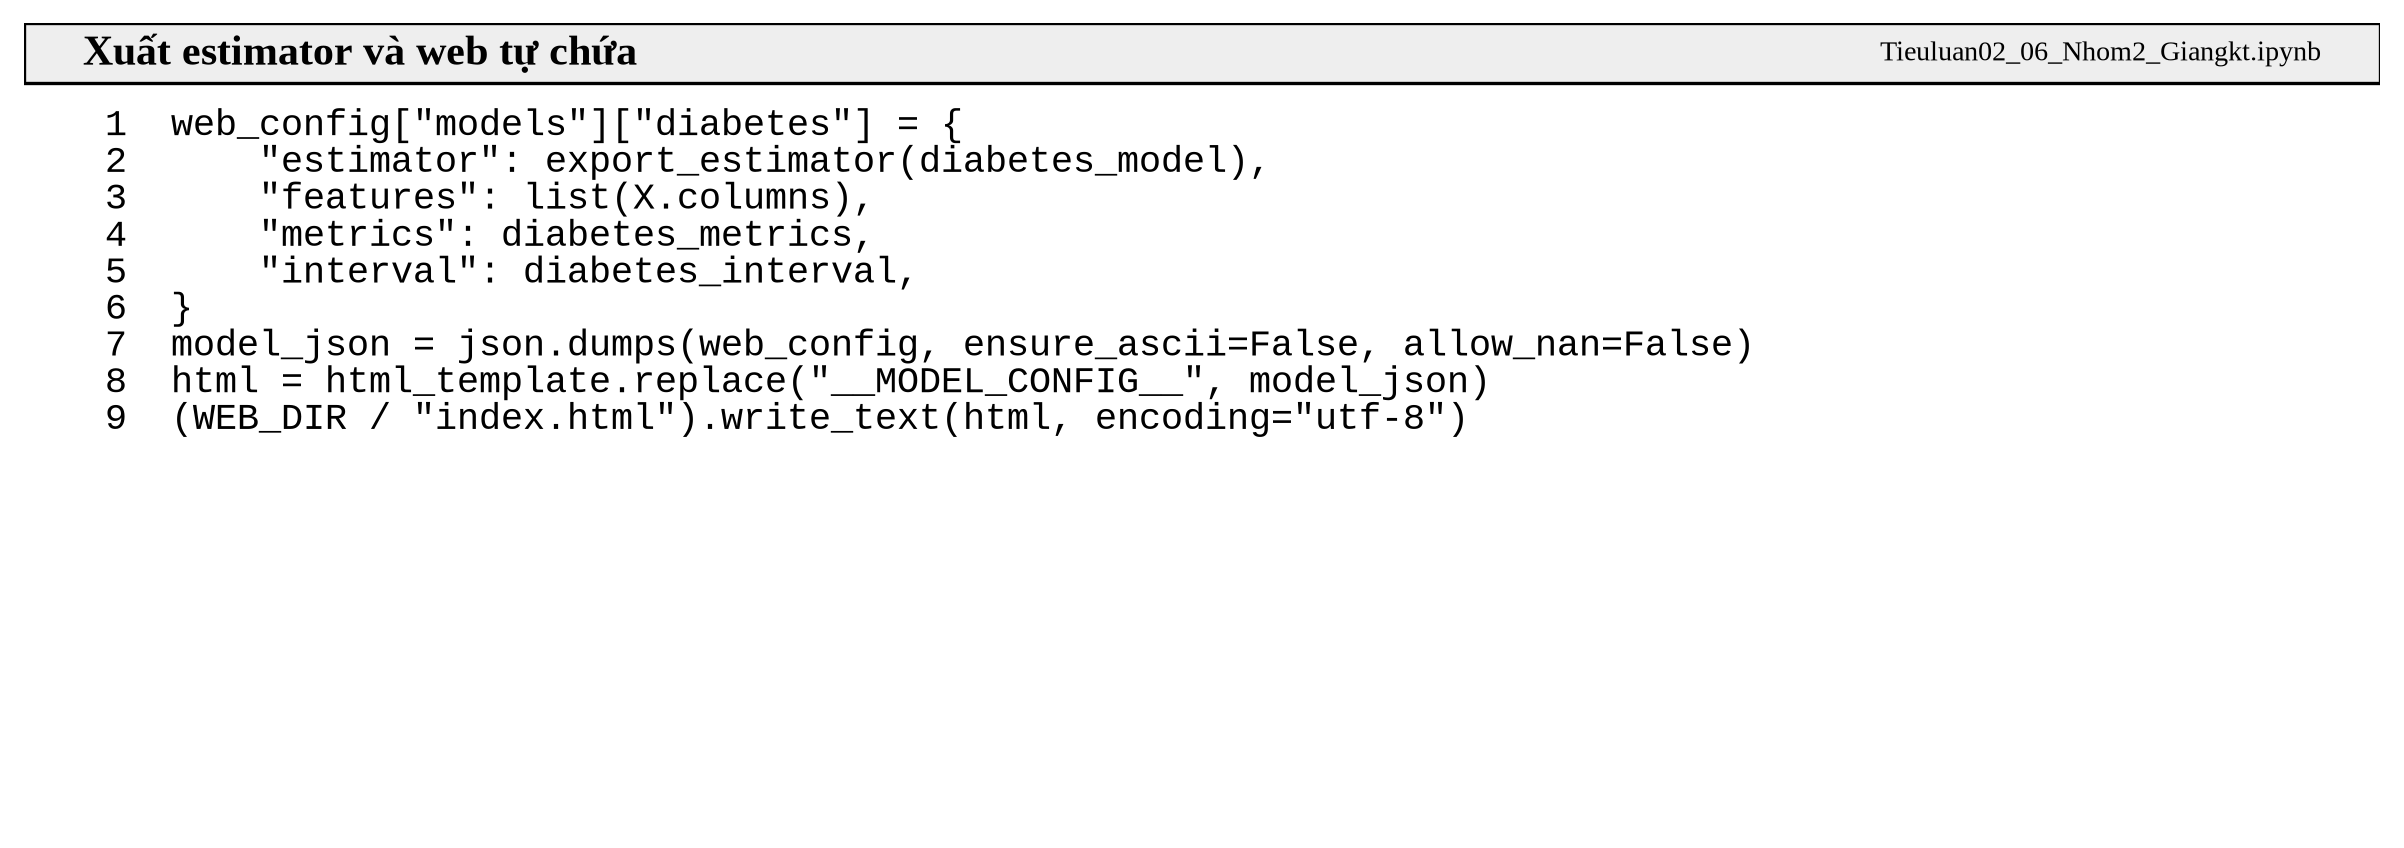
\includegraphics[width=\linewidth,height=.56\textheight,keepaspectratio]{media/media/image42.png}
\caption{Xuất estimator sang JavaScript}\label{fig:legacy-5.21}
\end{figure}



\subsection{Chatbot dự đoán, tư vấn và hỏi đáp}\label{chatbot-dux1ef1-ux111ouxe1n-tux1b0-vux1ea5n-vuxe0-hux1ecfi-ux111uxe1p}

Chatbot nhận đường huyết, HbA1c, BMI, tuổi, huyết áp tâm thu/tâm trương,
huyết áp trung bình, cholesterol toàn phần, LDL, HDL, triglyceride và
các đặc trưng nghiên cứu s4/s5. Câu `huyết áp 90' được hỏi lại loại số
đo; thiếu đơn vị thì hỏi tiếp. Một tin nhắn có thể chứa nhiều chỉ số,
đơn vị được gắn riêng với từng giá trị để tránh lấy nhầm mmol/L của HDL
cho glucose.

Các ngưỡng xét nghiệm tham khảo NIDDK/ADA. Đường huyết thấp được xử lý
trước bảng phân loại đường cao. Sau bữa ăn thông thường không bị đánh
đồng với nghiệm pháp 75 g glucose. Thai kỳ và trẻ em cần bối cảnh riêng.
Câu hỏi kê liều thuốc được chuyển thành hướng dẫn trao đổi với bác sĩ.

Kho tri thức mở rộng thành 20 chủ đề, bổ sung nguồn AHA về huyết áp,
MedlinePlus về mỡ máu và Mayo Clinic về xét nghiệm cholesterol. Nội
dung, đường quan hệ KG và danh mục nguồn được xuất ra
health\_knowledge.json. BM25 truy xuất kết hợp bộ nhận diện số đo; chưa
kết nối LLM ngoài. Khi chia sẻ form, chatbot nhận đủ các trường đã nhập,
nhưng loại giá trị trung vị thay thế khỏi nhận xét y khoa. Mã giới tính
1/2 không tự dùng chọn ngưỡng HDL; s5 không tự quy đổi thành xét nghiệm
triglyceride. Hồ sơ chỉ giữ trong phiên.

\section{Đánh giá tổng hợp}\label{ux111uxe1nh-giuxe1-tux1ed5ng-hux1ee3p}

Kết quả cho thấy một notebook có thể bao quát tải dữ liệu, tiền xử lý,
KG, RAG, đánh giá, báo cáo và web. GraphRAG lai cung cấp thêm loại bằng
chứng mà Vector RAG không có: quan hệ có tên và đường đi giữa các thực
thể.

Đổi lại, KG yêu cầu thiết kế ontology, kiểm soát quan hệ và cập nhật
theo thời gian. Chi phí này chỉ đáng bỏ ra khi bài toán cần giải thích,
liên kết đa bước hoặc quản trị tri thức dài hạn.

Bài làm đạt mục tiêu nguyên mẫu tái lập. Hạn chế chính là corpus nhỏ,
đánh giá ít câu hỏi, generator dạng mẫu và chưa có chuyên gia miền thẩm
định. Những giới hạn này được ghi rõ thay vì suy rộng kết quả.

\subsection{Kết quả huấn luyện ba miền}\label{kux1ebft-quux1ea3-huux1ea5n-luyux1ec7n-ba-miux1ec1n}

\Needspace{7\baselineskip}
\captionof{table}{Tổng hợp kết quả giữ từ Tiểu luận 02}\label{tab:legacy-5.1}

{\def\LTcaptype{none} % do not increment counter
\begin{longtable}[]{@{}
  >{\raggedright\arraybackslash}p{(\linewidth - 8\tabcolsep) * \real{0.1875}}
  >{\centering\arraybackslash}p{(\linewidth - 8\tabcolsep) * \real{0.2813}}
  >{\centering\arraybackslash}p{(\linewidth - 8\tabcolsep) * \real{0.1750}}
  >{\centering\arraybackslash}p{(\linewidth - 8\tabcolsep) * \real{0.1750}}
  >{\centering\arraybackslash}p{(\linewidth - 8\tabcolsep) * \real{0.1813}}@{}}
\toprule\noalign{}
\begin{minipage}[b]{\linewidth}\raggedright
\textbf{Miền}
\end{minipage} & \begin{minipage}[b]{\linewidth}\centering
\textbf{Mô hình}
\end{minipage} & \begin{minipage}[b]{\linewidth}\centering
\textbf{CV MAE}
\end{minipage} & \begin{minipage}[b]{\linewidth}\centering
\textbf{Test MAE}
\end{minipage} & \begin{minipage}[b]{\linewidth}\centering
\textbf{R2}
\end{minipage} \\
\midrule\noalign{}
\endhead
\bottomrule\noalign{}
\endlastfoot
diabetes & Ridge & 44.443 & 42.936 & 0.452 \\
stock & Persistence & 1215.974 & 728.128 & 0.871 \\
gold & SVR return & 38.792 & 49.440 & 0.880 \\
\end{longtable}
}

Mô hình được chọn theo CV MAE trên tập train. Chỉ số test được tính trên
phần dữ liệu giữ lại.

\subsection{Kết quả truy xuất và bộ ba tri thức}\label{kux1ebft-quux1ea3-truy-xuux1ea5t-vuxe0-bux1ed9-ba-tri-thux1ee9c}

\Needspace{7\baselineskip}
\captionof{table}{Kết quả smoke test được giữ nguyên}\label{tab:legacy-5.2}

{\def\LTcaptype{none} % do not increment counter
\begin{longtable}[]{@{}
  >{\raggedright\arraybackslash}p{(\linewidth - 8\tabcolsep) * \real{0.5000}}
  >{\centering\arraybackslash}p{(\linewidth - 8\tabcolsep) * \real{0.1501}}
  >{\centering\arraybackslash}p{(\linewidth - 8\tabcolsep) * \real{0.1125}}
  >{\centering\arraybackslash}p{(\linewidth - 8\tabcolsep) * \real{0.1125}}
  >{\centering\arraybackslash}p{(\linewidth - 8\tabcolsep) * \real{0.1250}}@{}}
\toprule\noalign{}
\begin{minipage}[b]{\linewidth}\raggedright
\textbf{Câu hỏi}
\end{minipage} & \begin{minipage}[b]{\linewidth}\centering
\textbf{Miền}
\end{minipage} & \begin{minipage}[b]{\linewidth}\centering
\textbf{P@3}
\end{minipage} & \begin{minipage}[b]{\linewidth}\centering
\textbf{Graph}
\end{minipage} & \begin{minipage}[b]{\linewidth}\centering
\textbf{Hybrid}
\end{minipage} \\
\midrule\noalign{}
\endhead
\bottomrule\noalign{}
\endlastfoot
Theo dõi gì khi quản lý bệnh tiểu đường? & diabetes & 0.67 & 1 & 0.92 \\
Mô hình tiểu đường có sai số bao nhiêu? & diabetes & 0.33 & 1 & 0.58 \\
Giá FPT gần nhất và RSI là bao nhiêu? & stock & 0.67 & 1 & 0.92 \\
MA20 của cổ phiếu có ý nghĩa gì? & stock & 0.33 & 1 & 0.58 \\
Giá vàng gần nhất là bao nhiêu? & gold & 0.33 & 1 & 0.58 \\
Fed, USD và địa chính trị ảnh hưởng vàng ra sao? & gold & 0.67 & 1 &
0.92 \\
\end{longtable}
}

Bảng này là phép kiểm tra hồi quy cho pipeline. Nó không thay thế đánh
giá câu trả lời bởi chuyên gia.

\Needspace{7\baselineskip}
\captionof{table}{Bộ ba tri thức của hệ thống}\label{tab:legacy-5.3}

{\def\LTcaptype{none} % do not increment counter
\begin{longtable}[]{@{}
  >{\raggedright\arraybackslash}p{(\linewidth - 4\tabcolsep) * \real{0.3250}}
  >{\centering\arraybackslash}p{(\linewidth - 4\tabcolsep) * \real{0.3625}}
  >{\centering\arraybackslash}p{(\linewidth - 4\tabcolsep) * \real{0.3125}}@{}}
\toprule\noalign{}
\begin{minipage}[b]{\linewidth}\raggedright
\textbf{Subject}
\end{minipage} & \begin{minipage}[b]{\linewidth}\centering
\textbf{Predicate}
\end{minipage} & \begin{minipage}[b]{\linewidth}\centering
\textbf{Object}
\end{minipage} \\
\midrule\noalign{}
\endhead
\bottomrule\noalign{}
\endlastfoot
Bệnh đái tháo đường & ĐƯỢC\_\allowbreak THEO\_\allowbreak DÕI\_\allowbreak BẰNG & Theo dõi HbA1c \\
Bệnh đái tháo đường & CẦN\_\allowbreak TƯ\_\allowbreak VẤN\_\allowbreak BỞI & Bác sĩ chuyên khoa \\
Glucose & LIÊN\_\allowbreak QUAN\_\allowbreak ĐẾN & Bệnh đái tháo đường \\
BMI & LÀ\_\allowbreak YẾU\_\allowbreak TỐ\_\allowbreak NGUY\_\allowbreak CƠ\_\allowbreak CỦA & Bệnh đái tháo đường \\
Huyết áp & CẦN\_\allowbreak THEO\_\allowbreak DÕI\_\allowbreak KHI & Bệnh đái tháo đường \\
Tuổi & ĐIỀU\_\allowbreak CHỈNH\_\allowbreak NGUY\_\allowbreak CƠ & Bệnh đái tháo đường \\
Chế độ ăn & HỖ\_\allowbreak TRỢ\_\allowbreak QUẢN\_\allowbreak LÝ & Bệnh đái tháo đường \\
Vận động & HỖ\_\allowbreak TRỢ\_\allowbreak QUẢN\_\allowbreak LÝ & Bệnh đái tháo đường \\
FPT.VN & CÓ\_\allowbreak GIÁ\_\allowbreak GẦN\_\allowbreak NHẤT & Giá FPT 57,100 VND \\
MA20 & MÔ\_\allowbreak TẢ\_\allowbreak XU\_\allowbreak HƯỚNG\_\allowbreak NGẮN\_\allowbreak HẠN\_\allowbreak CỦA & FPT.VN \\
MA60 & MÔ\_\allowbreak TẢ\_\allowbreak XU\_\allowbreak HƯỚNG\_\allowbreak TRUNG\_\allowbreak HẠN\_\allowbreak CỦA & FPT.VN \\
RSI14 & ĐO\_\allowbreak ĐỘNG\_\allowbreak LƯỢNG\_\allowbreak CỦA & FPT.VN \\
Thanh khoản & PHẢN\_\allowbreak ÁNH\_\allowbreak MỨC\_\allowbreak QUAN\_\allowbreak TÂM\_\allowbreak ĐẾN & FPT.VN \\
Kết quả kinh doanh & CÓ\_\allowbreak THỂ\_\allowbreak TÁC\_\allowbreak ĐỘNG & FPT.VN \\
Tâm lý thị trường & CÓ\_\allowbreak THỂ\_\allowbreak TÁC\_\allowbreak ĐỘNG & FPT.VN \\
Vàng quốc tế GC=F & CÓ\_\allowbreak GIÁ\_\allowbreak GẦN\_\allowbreak NHẤT & Giá vàng 4,107.90 USD/oz \\
Vàng quốc tế GC=F & LÀ\_\allowbreak THAM\_\allowbreak CHIẾU\_\allowbreak CHO & Giá vàng SJC \\
Lãi suất Fed & CÓ\_\allowbreak QUAN\_\allowbreak HỆ\_\allowbreak NGHỊCH\_\allowbreak THƯỜNG\_\allowbreak GẶP\_\allowbreak VỚI & Vàng quốc tế
GC=F \\
Đồng USD & CÓ\_\allowbreak QUAN\_\allowbreak HỆ\_\allowbreak NGHỊCH\_\allowbreak THƯỜNG\_\allowbreak GẶP\_\allowbreak VỚI & Vàng quốc tế GC=F \\
Lạm phát & CÓ\_\allowbreak THỂ\_\allowbreak TĂNG\_\allowbreak NHU\_\allowbreak CẦU & Vàng quốc tế GC=F \\
Rủi ro địa chính trị & KÍCH\_\allowbreak HOẠT & Nhu cầu trú ẩn \\
Nhu cầu trú ẩn & CÓ\_\allowbreak THỂ\_\allowbreak HỖ\_\allowbreak TRỢ & Vàng quốc tế GC=F \\
\end{longtable}
}

\subsection{Chunking, embedding và giới hạn đánh giá}\label{chunking-embedding-vuxe0-giux1edbi-hux1ea1n-ux111uxe1nh-giuxe1}

Embedding là biểu diễn văn bản bằng vector; dense embedding học ngữ
nghĩa từ dữ liệu huấn luyện, còn TF-IDF là vector thưa theo tần suất từ.
Vector database bổ sung chỉ mục và quản trị truy vấn ở quy mô lớn;
prototype hiện lưu ma trận TF-IDF trong bộ nhớ, chưa vận hành một vector
database độc lập. Corpus gồm các tài liệu ngắn đã là đơn vị truy xuất,
nên không tạo hàng loạt chunk chồng lấn không cần thiết. Với PDF dài,
cần chunk theo heading, giữ metadata và thử kích thước/overlap bằng một
tập câu hỏi riêng.

Điểm hybrid cũ cộng 0,25 khi có bằng chứng đồ thị là điểm kỹ thuật tự
định nghĩa, không phải Accuracy, faithfulness hay xác suất đúng của câu
trả lời. Precision theo domain chỉ đo mức đúng miền. Việc mọi câu hỏi
tìm được một cạnh không chứng minh cạnh đó đủ để trả lời. Cần phân biệt
truy xuất văn bản, độ đúng đường đi và độ bám sát bằng chứng khi đánh
giá generator.

\subsection{Đồng bộ notebook và các chức năng web bổ sung}\label{ux111ux1ed3ng-bux1ed9-notebook-vuxe0-cuxe1c-chux1ee9c-nux103ng-web-bux1ed5-sung}

main.ipynb chứa các bước thực nghiệm mới, pipeline KG/RAG từ Tiểu luận
02, xuất mô hình và đóng gói web. Chế độ full là cấu hình của số liệu
trong báo cáo; quick dùng ít dữ liệu/epoch hơn để kiểm tra, không thay
số liệu full trong báo cáo. Manifest lưu seed, phiên bản thư viện, hash
dataset, checkpoint và cấu hình chạy.

Giao diện Insight Lab giữ khu dự đoán ba miền, trợ lý sức khỏe, màu sắc
và bố cục chính. Khu thực nghiệm bổ sung giá nhà, phân loại nhãn nguy cơ
tổng hợp, nhận dạng chữ số CNN và dự báo chuỗi. Các mô hình mới sử dụng
API /api/predict và trọng số JSON xuất từ notebook. API không gọi dịch
vụ LLM, không cần secret và có kiểm tra kích thước cũng như giá trị đầu
vào. Chatbot sức khỏe cũ vẫn xử lý trong trình duyệt; dữ liệu nhập vào
các demo API được gửi tới máy chủ inference để tính dự đoán.

\subsection{Theo dõi một câu hỏi qua các bước truy xuất}\label{theo-duxf5i-mux1ed9t-cuxe2u-hux1ecfi-qua-cuxe1c-bux1b0ux1edbc-truy-xuux1ea5t}

Xét câu hỏi ``Giá FPT gần nhất và RSI là bao nhiêu?''. Câu hỏi gồm một
thực thể FPT và hai nhu cầu thông tin: giá quan sát gần nhất, chỉ báo
RSI. Tìm đúng miền stock mới là bước đầu; muốn trả lời đủ cần các tài
liệu hoặc thuộc tính cung cấp cả hai giá trị và ngày dữ liệu. Prototype
không dùng điểm số tương đồng để tự sinh thêm một giá hoặc RSI chưa tồn
tại trong nguồn.

\begin{figure}[H]
\centering
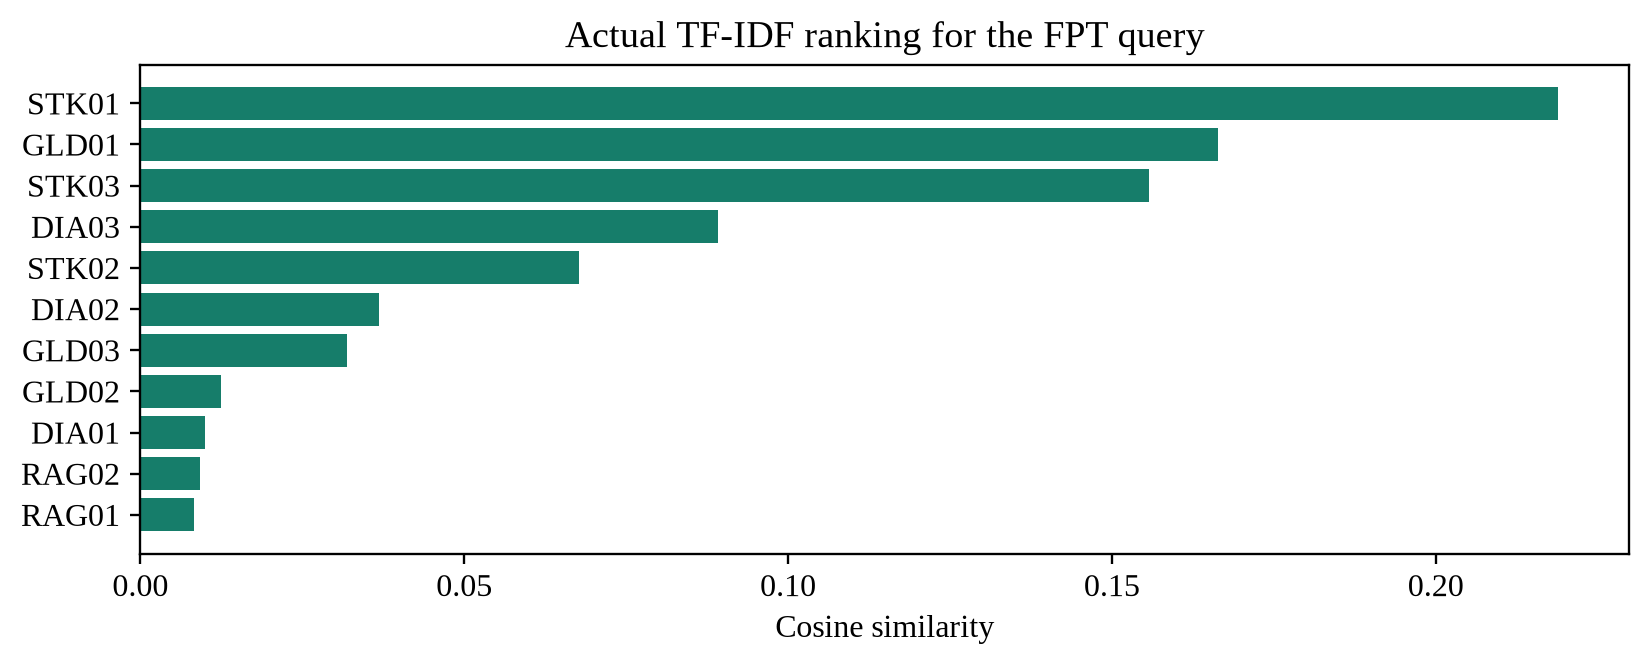
\includegraphics[width=\linewidth,height=.56\textheight,keepaspectratio]{media/media/image43.png}
\caption{Thứ hạng TF-IDF thực tế cho câu hỏi FPT trên toàn corpus}\label{fig:legacy-5.22}
\end{figure}



\Needspace{7\baselineskip}
\captionof{table}{Năm tài liệu đứng đầu của ví dụ truy xuất}\label{tab:legacy-5.4}

{\def\LTcaptype{none} % do not increment counter
\begin{longtable}[]{@{}
  >{\raggedright\arraybackslash}p{(\linewidth - 6\tabcolsep) * \real{0.1250}}
  >{\centering\arraybackslash}p{(\linewidth - 6\tabcolsep) * \real{0.3125}}
  >{\centering\arraybackslash}p{(\linewidth - 6\tabcolsep) * \real{0.2500}}
  >{\centering\arraybackslash}p{(\linewidth - 6\tabcolsep) * \real{0.3125}}@{}}
\toprule\noalign{}
\begin{minipage}[b]{\linewidth}\raggedright
\textbf{Hạng}
\end{minipage} & \begin{minipage}[b]{\linewidth}\centering
\textbf{Tài liệu}
\end{minipage} & \begin{minipage}[b]{\linewidth}\centering
\textbf{Miền}
\end{minipage} & \begin{minipage}[b]{\linewidth}\centering
\textbf{Cosine}
\end{minipage} \\
\midrule\noalign{}
\endhead
\bottomrule\noalign{}
\endlastfoot
1 & STK01 & stock & 0.218913 \\
2 & GLD01 & gold & 0.166334 \\
3 & STK03 & stock & 0.155685 \\
4 & DIA03 & diabetes & 0.089192 \\
5 & STK02 & stock & 0.067704 \\
\end{longtable}
}

Kết quả này cũng bộc lộ một lỗi truy xuất: GLD01 thuộc miền vàng đứng
thứ hai vì có nhiều từ chỉ dữ liệu thị trường gần với câu hỏi, trong khi
STK02 chứa thông tin chỉ báo FPT chỉ đứng thứ năm. Top-3 vì vậy chưa
cung cấp đủ bằng chứng cho phần RSI. Nếu chỉ ghép ba đoạn đầu, câu trả
lời không được tự bù một giá trị RSI. Lọc theo thực thể/miền hoặc tách
câu hỏi thành hai nhu cầu truy xuất là hướng sửa cần kiểm tra trên tập
câu hỏi riêng, không được coi là cải thiện đã đo trong lần chạy này.

Corpus thực nghiệm có 11 tài liệu và 508 đặc trưng TF-IDF
unigram/bigram. Query được transform bằng cùng vocabulary đã fit trên
corpus rồi tính cosine với từng dòng ma trận. Top-3 chỉ là một ngân sách
truy xuất; tài liệu thứ tư không trở thành sai về nội dung chỉ vì bị cắt
khỏi ngữ cảnh. Các điểm trong hình là kết quả tính thật, không phải xác
suất tài liệu đúng hoặc mức tin cậy của câu trả lời.

Bằng chứng STK01: Chuỗi FPT.VN gồm 1304 phiên từ 15/10/2021 đến
14/10/2026; giá đóng cửa gần nhất 57,100 VND.

Bằng chứng GLD01: Chuỗi vàng GC=F gồm 1257 phiên từ 15/10/2021 đến
14/10/2026; giá gần nhất 4,107.90 USD/oz.

Bằng chứng STK03: Đường trung bình động mô tả xu hướng quá khứ chứ không
bảo đảm giá tương lai. RSI là chỉ báo động lượng và cần kết hợp thanh
khoản, cơ bản doanh nghiệp cùng bối cảnh thị trường.

Nhánh đồ thị nhận diện miền và lấy các bộ ba liên quan để bổ sung quan
hệ giữa mã tài sản, chỉ báo và yếu tố tác động. NetworkX lưu đỉnh/cạnh
trong bộ nhớ; không có bước suy diễn tất cả đường đi hoặc xếp hạng cộng
đồng đồ thị quy mô lớn. Generator hiện ghép văn bản theo cấu trúc xác
định. Do đó cách gọi GraphRAG trong prototype chỉ mô tả việc bổ sung
bằng chứng đồ thị, không đồng nhất với một hệ thống GraphRAG dùng LLM để
trích xuất và tổng hợp cộng đồng.

Trong CSV bộ ba thật, FPT.VN nối với ``Giá FPT 57,100 VND'' qua quan hệ
CÓ\_GIÁ\_GẦN\_NHẤT; RSI14 nối tới FPT.VN qua ĐO\_ĐỘNG\_LƯỢNG\_CỦA. Cạnh
thứ hai chỉ xác định RSI14 đo động lượng của FPT, không chứa giá trị RSI
số. Vì thế nhánh đồ thị có thể bổ sung quan hệ nhưng chưa đủ thay tài
liệu STK02 bị bỏ khỏi top-3. Cần phân biệt bằng chứng về một quan hệ với
bằng chứng về một thuộc tính định lượng tại một thời điểm.

\subsection{Hai luồng hỏi đáp và giới hạn của câu trả lời}\label{hai-luux1ed3ng-hux1ecfi-ux111uxe1p-vuxe0-giux1edbi-hux1ea1n-cux1ee7a-cuxe2u-trux1ea3-lux1eddi}

Notebook truy xuất trên corpus đa miền ngắn, trong đó một phần tài liệu
thị trường được tạo từ bản chụp dữ liệu đã xử lý. Chatbot trên web lại là luồng
sức khỏe có corpus riêng, BM25, thực thể và trạng thái đối thoại. Hai
luồng dùng chung ý tưởng tìm bằng chứng trước khi trả lời nhưng không
dùng cùng chỉ mục, cùng số tài liệu hoặc cùng điểm đánh giá. Không lấy
Precision@3 của notebook làm độ chính xác cho chatbot web.

Trong web, câu hỏi được chuẩn hóa để tìm chủ đề; lịch sử đối thoại giữ
ngữ cảnh khi cần hỏi thêm đơn vị hoặc mục đích. Luật kiểm tra đơn vị
chạy trước các nhánh cần diễn giải chỉ số. Khi tìm được chủ đề, phần trả
lời đưa thông tin tham khảo, yếu tố liên quan và cảnh báo phạm vi. Khi
thiếu dữ liệu hoặc câu hỏi vượt khả năng, hệ thống phải nêu thiếu thông
tin thay vì tạo một kết luận chắc chắn.

Tình huống kiểm tra có thể bắt đầu bằng câu hỏi về HbA1c, sau đó hỏi
tiếp về một chỉ số glucose chưa có đơn vị để quan sát yêu cầu làm rõ.
Đây là kịch bản tương tác, không phải một hồ sơ bệnh nhân hoặc bằng
chứng về năng lực chẩn đoán. Nội dung sức khỏe được giới hạn ở giáo dục
và giải thích giao diện; không dùng dự đoán của classifier tổng hợp để
thay lời khuyên chuyên môn.

\productlink{Trợ lý hỏi đáp theo tài liệu}{https://rag-httm-chatbot.vercel.app/\#chatbot}

\subsection{Phân biệt ba miền dự đoán gốc và các mô hình bổ sung}\label{phuxe2n-biux1ec7t-ba-miux1ec1n-dux1ef1-ux111ouxe1n-gux1ed1c-vuxe0-cuxe1c-muxf4-huxecnh-bux1ed5-sung}

Khu dự đoán gốc có ba miền: hồi quy tiến triển bệnh trên bộ diabetes 442
mẫu, dự báo FPT và dự báo vàng với đặc trưng thị trường. Hồi quy y tế
trả một thang tiến triển bệnh của dataset, không phải nhãn
High/Low/Moderate của 50.000 mẫu tổng hợp ở Chương 2. Hai mô hình thị
trường gốc sử dụng đặc trưng được dựng từ lịch sử, trong khi Chương 4 sử
dụng 30 log-return và checkpoint recurrent riêng. Giao diện giữ cả hai
để đối chiếu phương pháp, không hợp nhất kết quả của chúng thành cùng
một phép thử.

Để dùng khu gốc, chọn miền, kiểm tra nhãn và đơn vị từng trường rồi chạy
dự đoán. Các giá trị mặc định của thị trường dựa trên bản chụp dữ liệu đi kèm
cấu hình. Nếu sửa đặc trưng thủ công, người dùng đang tạo kịch bản;
không được hiểu đầu ra là cập nhật giá thời gian thực. Phần KG bổ trợ
cách đọc yếu tố và quan hệ; nó không tự sửa sai số của regressor hoặc
tạo chứng cứ cho một dự báo chưa có nhãn thực.

\productlink{Thực nghiệm trên ba miền dữ liệu}{https://rag-httm-chatbot.vercel.app/\#predict}

\subsection{Đường triển khai, kiểm thử và khả năng tái lập}\label{ux111ux1b0ux1eddng-triux1ec3n-khai-kiux1ec3m-thux1eed-vuxe0-khux1ea3-nux103ng-tuxe1i-lux1eadp}

Mô hình mới được huấn luyện trong notebook, lưu checkpoint và xuất tham
số sang JSON nén. Vercel nạp bundle để chạy suy luận bằng Python
standard library, không train lại theo yêu cầu người dùng. Rừng cây giữ
ngưỡng và lá; CNN giữ kernel/dense; recurrent giữ trọng số cổng và tham
số scale. Các tham số tiền xử lý được xuất cùng mô hình để tránh dùng
một phép biến đổi khác giữa notebook và web.

Đối chiếu suy luận không chỉ kiểm tra nhãn cuối: 30 vector bảng so sánh
giá hoặc điểm theo lớp, sáu ảnh so sánh toàn bộ logits, sáu checkpoint
recurrent so sánh giá dự đoán. Sai lệch số thực được kiểm tra với ngưỡng
nhỏ trong test tự động. Trường hợp float32 của cây và thứ tự cổng GRU
được xử lý theo đúng thư viện train; đây là những chi tiết có thể gây
sai kết quả dù giao diện vẫn hoạt động bình thường.

Kiểm thử âm gồm ảnh trống, sai số pixel, NaN/Infinity, giá trị số sai
kiểu, chuỗi thiếu phần tử và miền không tồn tại. Kiểm thử trình duyệt
xác nhận thao tác chọn ảnh, chạy API, đổi miền và trạng thái lỗi. Các
kiểm tra này chứng minh đường xử lý thực thi đúng các trường hợp đã thử,
không thay thế đánh giá thống kê ngoài mẫu. Mọi lần thay đổi trọng số
hoặc preprocessing cần xuất bundle và chạy lại đối chiếu.

Mỗi biểu đồ phân tích mới có danh sách tệp đầu vào và SHA-256 trong
figure\_lineage.json. Các CSV prediction, lịch sử train và phép chia
được giữ để tính lại bảng kết quả. Các sơ đồ có nhãn minh họa cơ chế chỉ
giải thích luồng tính toán; chúng không được xem là ảnh dữ liệu thu
thập. Cách tổ chức này cho phép kiểm tra báo cáo từ kết quả số trở về mã
và dữ liệu thay vì chỉ dựa vào mô tả bằng lời.

Web: \url{https://rag-httm-chatbot.vercel.app/}

GitHub: \url{https://github.com/jellalaz/HTTM_ThayQue}

\section{Kết luận chương}\label{kux1ebft-luux1eadn-chux1b0ux1a1ng-1}

Điều quan trọng nhất rút ra là không nên coi GraphRAG như một nhãn công
nghệ thay thế cho thiết kế dữ liệu. Chất lượng câu trả lời bắt đầu từ
việc định nghĩa thực thể, quan hệ, nguồn và phạm vi kết luận. Notebook
và web dùng chung artifact để đối chiếu kết quả.
